% !TEX program = pdflatex
% !TEX encoding = UTF-8 Unicode

% Plantilla, basada en la clase `scrbook` del paquete KOMA-script,  para la elaboración de un TFG siguiendo las directrices del la comisión del Grado en Matemáticas de la Universidad de Granada.

% Francisco Torralbo Torralbo

\documentclass[print, color]{ugrTFG}

% VERSIÓN ELECTRÓNICA PARA TABLETA
% Cambiando la opción "print" por "tablet" generaremos un pdf adaptado para leerlo en tabletas de 9 pulgadas.

% -------------------------------------------------------------------
% INFORMACIÓN DEL TFG Y EL AUTOR
% -------------------------------------------------------------------

\newcommand{\miTitulo}{Análisis teórico y empírico del Deep Double Descent\xspace}
\newcommand{\miNombre}{Juan Antonio Ruiz Arévalo\xspace}
\newcommand{\miGrado}{Doble Grado en Ingeniería Informática y Matemáticas}
\newcommand{\miFacultad}{Escuela Técnica Superior de Ingenierías Informática y de Telecomunicación y Facultad de Ciencias}
\newcommand{\miUniversidad}{Universidad de Granada}
\newcommand{\misTutores}{\newline Francisco Javier Merí de la Maza \\ Pablo Mesejo Santiago\newline}

% Añadir tantos tutores como sea necesario separando cada uno de ellos mediante el comando `\medskip` y una línea en blanco
\newcommand{\miTutor}{
  Francisco Javier Merí de la Maza \\ \emph{Departamento de Análisis Matemático} 

  % Añadir tantos tutores como sea necesario. 

  \medskip
  Pablo Mesejo Santiago \\ \emph{Departamento de Ciencias de la Computación e Inteligencia Artificial}
}
\newcommand{\miCurso}{2024-2025\xspace}

\hypersetup{
	pdftitle={\miTitulo},
	pdfauthor={\textcopyright\ \miNombre, \miFacultad, \miUniversidad}
}

\let\cleardoublepage\clearpage

\usepackage{subcaption}
\usepackage{multirow}
\usepackage{colortbl} 
\usepackage{xcolor}   
\usepackage{nicematrix}
\usepackage{graphicx}
\usepackage{eurosym}
\usepackage{pifont}

\newcommand{\cmark}{\ding{51}} 
\newcommand{\xmark}{\ding{55}} 

\begin{document}

\maketitle

% -------------------------------------------------------------------
% FRONTMATTER
% -------------------------------------------------------------------
\frontmatter % Desactiva la numeración de capítulos y usa numeración romana para las páginas

% !TeX root = ../tfg.tex
% !TeX encoding = utf8
%
%*******************************************************
% Declaración de originalidad
%*******************************************************

\thispagestyle{empty}

\hfill\vfill

\textsc{Declaración de originalidad}\\\bigskip

D. \miNombre \\\medskip

Declaro explícitamente que el trabajo presentado como Trabajo de Fin de Grado (TFG), correspondiente al curso académico \miCurso, es original, entendido esto en el sentido de que no he utilizado para la elaboración del trabajo fuentes sin citarlas debidamente.
\medskip

En Granada a \today 
\vspace{3cm}
\begin{center} 
Fdo: \miNombre 

\end{center}

\vfill

\clearpage
\endinput
   
% !TeX root = ../tfg.tex
% !TeX encoding = utf8

%*******************************************************
% Dedication
%*******************************************************
\thispagestyle{empty}
\phantomsection 
\pdfbookmark[1]{Dedicatoria}{Dedicatoria}

\hfill
\vfill

\begin{flushright}
\emph{A mis padres, a mi hermana \\ y a toda mi familia.} \\
\end{flushright}

\vfill

\clearpage

\endinput
                % Opcional
% !TeX root = ../tfg.tex
% !TeX encoding = utf8

%*******************************************************
% Agradecimientos
%*******************************************************

\chapter{Agradecimientos}

\emph{Agradecimientos}

\clearpage
\thispagestyle{empty}
\mbox{}
\newpage
\endinput

            % Opcional

% !TeX root = ../tfg.tex
% !TeX encoding = utf8
%
%*******************************************************
% Resumen
%*******************************************************

\chapter{Resumen}

\noindent\textbf{Palabras clave:} Aprendizaje Automático, Aprendizaje Profundo, Inteligencia Artificial, Sesgo-Varianza, Aproximación No Lineal, Visión por Computador

\

El aprendizaje automático, y en particular el aprendizaje profundo, se ha convertido en una herramienta fundamental en numerosos ámbitos, desempeñando un papel determinante al complementar e incluso reemplazar las labores humanas en diversos contextos. No obstante, el entrenamiento de modelos cada vez más complejos ha revelado, recientemente, comportamientos inesperados en su rendimiento, entre los cuales destaca el fenómeno conocido como \emph{Deep Double Descent}. Este comportamiento desafía la sabiduría clásica del aprendizaje, al evidenciar que la relación entre la complejidad del modelo y su rendimiento no se ajusta a las curvas tradicionales previstas por la teoría convencional.\newline

En el enfoque clásico del aprendizaje automático, aumentar la capacidad de un modelo mejora su capacidad para ajustarse a los datos, pero eventualmente conduce al sobreajuste, momento en el cual el rendimiento del modelo comienza a empeorar. En contraposición, hallazgos recientes han demostrado que, a medida que el modelo sigue aumentando su capacidad más allá de ese sobreajuste, su rendimiento comienza a mejorar nuevamente, creando un segundo descenso que rompe con la intuición clásica. Este comportamiento revela una brecha significativa entre los conocimientos teóricos y los resultados empíricos observados en la actualidad, lo cual nos recuerda que el campo de la inteligencia artificial está en constante evolución, y que los avances en esta disciplina no se producen de forma paralela entre la teoría y la práctica.\newline

En este TFG, nos centraremos en exponer los principios informáticos y matemáticos esenciales para comprender el \emph{Deep Double Descent}, partiendo del marco clásico del equilibrio entre sesgo y varianza, para lo cual será necesario recurrir a nociones de teoría de la probabilidad y estadística. Asimismo, se revisarán e introducirán conceptos relativos al álgebra matricial que resultan imprescindibles para entenderlo en profundidad. De esta manera, el objetivo principal del trabajo consiste en dar a conocer el conocimiento disponible hasta la fecha para explicar este suceso, complementándolo con la realización de diversos experimentos que respalden empíricamente la información teórica, con el fin de discutir algunas de las preguntas abiertas que plantea la literatura actual.\newline

Por otro lado, se desarrollará la teoría de la aproximación no lineal, dada su a priori y significativa relación con el \emph{Deep Double Descent}, resaltando las distintas analogías que comparten. Con todo ello, se busca contribuir a la construcción de un puente que permita reconciliar la sabiduría clásica con los descubrimientos modernos, favoreciendo así una comprensión más unificada del aprendizaje automático contemporáneo.\newline
% !TeX root = ../tfg.tex
% !TeX encoding = utf8
%
%*******************************************************
% Summary
%*******************************************************

\selectlanguage{english}
\chapter{Summary}

\noindent\textbf{Keywords:} Machine Learning, Deep Learning, Artificial Intelligence, Bias-Variance, Non-Linear Approximation, Generalization Frameworks, Explainability

\

Machine learning, particularly deep learning, has become a fundamental tool in many fields, playing a decisive role in complementing and even replacing human work in various contexts. However, the training of increasingly complex models has recently revealed unexpected behaviors in their performance, among which the phenomenon known as \emph{Deep Double Descent} stands out. This behavior challenges the classical wisdom of learning by showing that the relationship between model complexity and performance does not conform to the learning curves predicted by conventional theory.

The classical concepts of learning are insufficient to explain certain emerging phenomena. In fact, some of them, such as the bias-variance trade-off, seem to contradict these new trends. This event reveals a significant gap between theoretical knowledge and the empirical findings recorded in recent observations, which reminds us that the field of AI is constantly evolving, and that advances in this discipline do not occur in parallel between theory and practice.

In this Final Degree Project, we will focus on exposing the underlying computational and mathematical principles necessary to understand the \emph{Deep Double Descent}, starting from the classical framework of the bias-variance trade-off, for which it will be necessary to draw on notions of probability and statistics. Likewise, concepts related to matrix algebra, which are essential for a deeper understanding, will be reviewed and introduced. However, given the common perception of neural networks as «black boxes», due to the fact that their inner workings are not precisely known, we will work in an alternative way by defining techniques that will help to explain their behavior.

This study focuses on the definition of new generalization frameworks, known as inductive biases, that provide explanability beyond what is offered by classical theory, thus unifying traditional concepts with modern approaches. In addition, the nonlinear approach is used as a complementary way to reinforce these frameworks from a more mathematical and formal perspective.

Through various experiments, both in simple architectures and in advanced convolutional architectures such as ResNet, it is shown that this phenomenon not only improves the performance of the models in classification and regression tasks, but also suggests that the solutions obtained tend to be increasingly simpler, following the philosophy of Ockham's razor principle.

In conclusion, this work is not only focused on providing an explanation of the \emph{Deep Double Descent}, but also constitutes an advance towards the understanding and explainability of the new generalization trends currently observed. This behavior suggests a new perspective on the direction that machine learning should take to achieve increasingly accurate results, based on the use of models with increasing capacity, following the logic that, in this context, \emph{«bigger is better»}.

\clearpage
\thispagestyle{empty}
\mbox{}
\newpage
% Al finalizar el resumen en inglés, volvemos a seleccionar el idioma español para el documento
\selectlanguage{spanish} 
\endinput
                    

% !TeX root = ../tfg.tex
% !TeX encoding = utf8

%*******************************************************
% Table of Contents
%*******************************************************
\phantomsection
\pdfbookmark[0]{\contentsname}{toc}

\setcounter{tocdepth}{2} % <-- 2 includes up to subsections in the ToC
\setcounter{secnumdepth}{3} % <-- 3 numbers up to subsubsections

\tableofcontents 

%*******************************************************
% List of Figures and of the Tables
%*******************************************************

    % *******************************************************
    %  List of Figures
    % *******************************************************    
    \phantomsection 
    \listoffigures

    %*******************************************************
    % List of Tables
    %*******************************************************
    \phantomsection 
    \listoftables
    
    %*******************************************************
    % List of Listings
    % The package \usepackage{listings} is needed
    %*******************************************************      
	  % \phantomsection 
    % \renewcommand{\lstlistlistingname}{Listados de código}
    % \lstlistoflistings 
\clearpage
\thispagestyle{empty}
\mbox{}
\newpage
            
% !TeX root = ../tfg.tex
% !TeX encoding = utf8
%
%*******************************************************
% Introducción
%*******************************************************

% \manualmark
%\markboth{\textsc{Introducción}}{\textsc{Introducción}} 

\chapter{Introducción}

En los últimos años, el \emph{Deep Double Descent} ha surgido como un importante campo de interés en el aprendizaje automático. La sabiduría tradicional sugiere que, a medida que aumenta la complejidad del modelo, el error fuera de la muestra disminuye inicialmente hasta alcanzar un mínimo y, a continuación, aumenta debido al sobreajuste, formando la tradicional curva con forma de ``U''. Este concepto tradicional del aprendizaje automático, conocido como equilibrio entre sesgo y varianza, difiere de las recientes observaciones obtenidas, que cuestionan este punto de vista, especialmente en modelos de aprendizaje profundo, en los que puede producirse una segunda disminución del error fuera de la muestra y alcanzar un nuevo mínimo, formando una nueva curva en la gráfica del error de generalización que presenta dos descensos. Este novedoso descubrimiento pone en tela de juicio la sabiduría clásica sobre el tema y proporciona nuevas perspectivas a la hora de crear y entrenar los modelos.\newline

Este trabajo de fin de grado se centra en explorar el concepto del \emph{Deep Double Descent}, sus fundamentos teóricos y sus implicaciones para el aprendizaje automático moderno. Un área clave de interés es cómo este fenómeno se manifiesta en redes neuronales profundas, conocidas por su enorme complejidad en cuanto a número de párametros se refiere y su potencial de sobreajuste.\newline

A pesar de que los modelos de aprendizaje profundo han tenido gran éxito en diversas aplicaciones, como la visión por computador o el procesamiento de lenguaje natural, la curva del doble descenso aporta nuevos conocimientos sobre cómo estos modelos pueden llegar a generalizar en un régimen que ha sido vagamente estudiado y explorado: el régimen sobreparametrizado.\newline

La idea clave es la existencia de dos zonas de actuación del modelo claramente diferenciadas, la zona infraparametrizada y la zona sobreparametrizada. Sin embargo, formalizar esta idea es significativamente complejo, dado que los modelos profundos funcionan como ``cajas negras'', lo que hace que, a medida que aumenta su complejidad, resulte cada vez más difícil interpretar y analizar su funcionamiento interno.\newline

Aunque cada vez hay más estudios abordando el suceso, muchos de ellos se centran en una perspectiva empírica del mismo, sin ofrecer una base teórica suficiente, mientras que otros sistematizan conceptos sin llegar a conclusiones prácticas. Con este trabajo buscamos cerrar la brecha entre la teoría y la práctica unificando explicaciones teóricas suficientemente rigurosas con ejemplos empíricos del mundo real con el objetivo de ofrecer una comprensión lo más completa posible.\newline


\section{Definición del problema}

\begin{figure}[h]
    \centering
    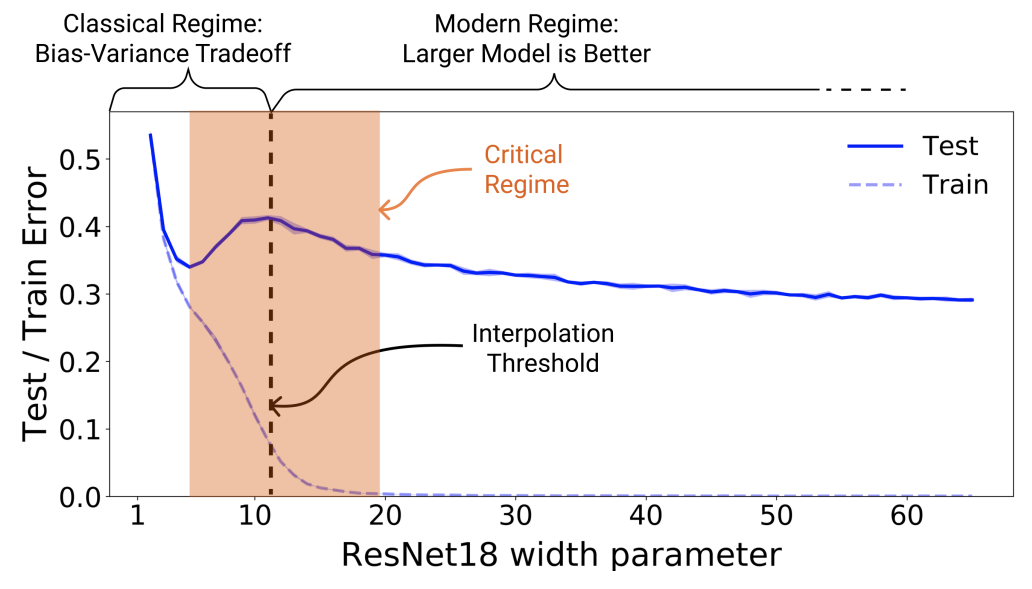
\includegraphics[width=0.8\textwidth]{img/problem-definition.png}
    \caption[Ejemplo de doble descenso profundo en ResNet18~\cite{Nakkiran2019}.] {Ejemplo de doble descenso en ResNet18~\cite{Nakkiran2019}. La imagen muestra el error de entrenamiento (\textit{train error}) y de generalización (\textit{test error}) para la arquitectura ResNet18 con diferente capacidad (número de parámetros). En ella, observamos las tres regiones de actuación del modelo claramente diferenciadas, así como el máximo del error de generalización correspondiente al umbral de interpolación y los dos descensos de la curva de dicho error.}\label{fig:ejemplo-definicion-double-descent}
\end{figure}

El término \emph{doble descenso profundo (deep double descent,~\cite{Belkin2019})} describe la forma que toma la curva del error de generalización (error fuera de la muestra) de un modelo de aprendizaje como función de la capacidad del mismo. De manera intuitiva, podemos distinguir 3 zonas o regiones diferenciadas en dicha curva:

\begin{itemize}
    \item \textbf{Región clásica (infraparametrizada):} En esta región, el modelo no es capaz de capturar toda la complejidad subyacente de la distribución de los datos debido a su baja capacidad. Como resultado, el error de generalización disminuirá inicialmente, ligado al hecho de que el modelo aprende de los datos de entrenamiento. Sin embargo, llegado un momento, el error de generalización aumentará de manera progresiva (véase \autoref{fig:ejemplo-definicion-double-descent}) dando lugar a la clásica curva en forma de ``U'', relacionado con el hecho de que el modelo, en lugar de seguir aprendiendo de los datos y obtener patrones de los mismos, memoriza los datos de entrenamiento.

    \item \textbf{Región moderna (sobreparametrizada):} En esta región, el modelo tiene una capacidad mayor de la necesaria para ajustar los datos de entrenamiento, es decir, dispone de suficientes herramientas (parámetros) para ajustar cada uno de los datos de entrenamiento. Contrariamente a lo que se esperaría según la sabiduría convencional, el error de generalización no necesariamente aumenta en este región y, bajo ciertas condiciones, dicho error puede reducirse nuevamente, produciendo un nuevo descenso de la curva del error de generalización que se conoce como \emph{doble descenso}.
    
    \item \textbf{Región crítica:} Esta región marca la transición entre la región infraparametrizada y la región sobreparametrizada y engloba zonas de ambas regiones. Dentro de ella, se encuentra el llamado umbral de interpolación o \textit{interpolation threshold}, que corresponde al punto donde el modelo tiene justo la capacidad suficiente para ajustar de manera prácticamente perfecta los datos de entrenamiento. En este punto crítico, el error de generalización alcanzará su máximo.\newline
       
\end{itemize}

Este doble descenso puede llegar a suponer la obtención de un nuevo mínimo en la curva del error de generalización, es decir, la obtención de modelos cuyas predicciones sean aún mejores. Sin embargo, se abre la puerta a la investigación del por qué ocurre este novedoso fenómeno, además de que tendremos que replantearnos algunas respuestas, tradicionalmente correctas, ante preguntas clásicas del aprendizaje profundo.\newline

\section{Motivación}

En el ámbito del aprendizaje automático, es de cultura general conocer la existencia de una brecha entre el desarrollo empírico y la fundamentación teórica subyacente. Los modelos modernos, en particular las redes neuronales profundas, han demostrado resultados sorprendentes~\cite{Sejnowski2020TheUE, He2020RecentAI} desde la generación de imágenes realistas mediante redes generativas~\cite{Elasri2022, Ruthotto2021} hasta el procesamiento de lenguaje natural (\textit{Natural Language Processing, NLP})~\cite{Kamath2019, Lauriola2022}. Sin embargo, estos resultados se logran sin una adecuada comprensión teórica~\cite{Ben-David2009, Berner2022}.\newline

Esta capacidad para obtener resultados que consideramos satisfactorios ha llevado a un enfoque predominantemente práctico, donde los avances se suelen producir de manera más rápida a través del ensayo y error y no tanto a través de modelos matemáticos bien fundamentados, lo que impide comprender, desde una perspectiva teórica, tanto la eficacia como las verdaderas limitaciones de estos modelos. El doble descenso plantea cuestiones sobre la sostenibilidad de este enfoque práctico y la necesidad de desarrollar un marco teórico que permita anticipar y guiar estos avances en lugar de simplemente reaccionar ante ellos.\newline

Aunque existen elogiosos esfuerzos para comprender las bases teóricas del deep learning~\cite{Zhang2021,Mallat2016, Prince2023, Bishop2023, Berner2022, Balestriero2018, Michael2018}, la desconexión entre avances teóricos y prácticos continúa siendo notable. Por ello, en los últimos años han ido apareciendo discrepancias, y se han observado fenómenos de carácter práctico, que han desafiado el conocimiento teórico tradicional. Es aquí donde se enmarca el concepto del \emph{Deep Double Descent}.\newline

De igual manera, este proyecto tiene una relevancia crucial, ya que podría transformar la forma en que se diseñan y optimizan los modelos profundos. Tradicionalmente, el enfoque clásico sugiere que, a medida que se aumenta la complejidad del modelo, este tiende a sobreajustarse a los datos, lo que limita su capacidad de generalización frente a nuevos datos no vistos y motivaba a optar por modelos más simples. Sin embargo, con la aparición del \textit{Deep Double Descent}, se ha demostrado que, más allá del sobreajuste, los modelos no solo continúan mejorando su capacidad de generalización, logrando mejores predicciones, sino que incluso mejoran, alcanzando una generalización aún mejor a la inicial.\newline 

Este descubrimiento sugiere que, siguiendo este enfoque, podríamos prescindir de la teoría clásica y centrarnos en desarrollar modelos más complejos. No obstante, las limitaciones computacionales y energéticas siguen representando un desafío en el entrenamiento de grandes modelos de deep learning ~\cite{Thompson2022, Cottier2025}. Por ello, en la actualidad, aún se aplican técnicas de regularización para mitigar el sobreajuste y optimizar el uso de recursos.\newline

En conclusión, el \emph{Deep Double Descent} representa un cambio de paradigma, digno de estudio, en el aprendizaje automático. Comprender los principios subyacentes permitiría avanzar en nuestra comprensión teórica del aprendizaje automático, reduciendo la brecha teórico-práctica, e incluso podría contribuir a guiar el diseño y optimización de modelos prácticos más efectivos.\newline

\section{Objetivos}

Los primeros indicios del \textit{Deep Double Descent} se remontan a la década de $1990$ y principios de los años $2000$~\cite{Opper1995,Opper2001}, aunque no se utilizaba específicamente esa terminología. Estos estudios mostraban la relación entre la complejidad del modelo y el error de generalización, indicando que, en algunos casos, aumentar la complejidad del modelo más allá de cierto punto no incrementaba necesariamente el error de generalización. Además, sentaron las bases para la comprensión moderna del suceso observado en modelos profundamente sobreparametrizados.\newline

No obstante, no es hasta $2019$ cuando Belkin et.\ al en~\cite{Belkin2019} abordan la primera investigación formal sobre este tema y le asignan su particular nombre. A partir de ese momento, la comunidad científica comienza a mostrar un creciente interés hasta el día de hoy, lo que nos lleva a catalogarlo como un acontecimiento novedoso.\newline

Por tanto, el objetivo principal de este TFG radica en tratar de ofrecer una explicación detallada y estructurada del reciente concepto del \emph{Deep Double Descent}. Este estudio se centrará en proporcionar una visión actualizada y rigurosa de sus fundamentos teóricos, implicaciones prácticas y relevancia en el desarrollo de modelos modernos, asegurando que el contenido se mantenga en concordancia con los avances más recientes en la investigación.\newline

Para alcanzar este objetivo, se han definido dos líneas de trabajo interrelacionadas: una orientada al desarrollo \textbf{matemático} y otra enfocada a la parte \textbf{informática}. Ambas se desarrollan de manera conjunta y complementaria, de modo que los avances teóricos guían y fundamentan la implementación práctica, mientras que los resultados experimentales permiten validar y enriquecer la comprensión teórica. A su vez, cada una de estas líneas de trabajo se descompone en una serie de objetivos parciales que, en conjunto, dirigen el desarrollo del proyecto.\newline

\subsection{Objetivo matemático}

El objetivo fundamental para la parte matemática consiste en profundizar en la comprensión teórica del \textit{Deep Double Descent} a través del estudio detallado de sus fundamentos matemáticos, explorando las relaciones con conceptos clásicos como el equilibrio sesgo-varianza y su posible conexión con la teoría de la aproximación no lineal. Con el fin de abordar de forma sistemática las distintas fases de este análisis, el presente objetivo se descompondrá en los siguientes objetivos parciales:

\begin{itemize}
    \item Realizar un análisis exhaustivo y detallado del estado del arte, revisando las principales teorías, descubrimientos y avances matemáticos relacionados.
    \item Presentar de manera detallada las teorías y enfoques tradicionales que, a día de hoy, prevalecen en la literatura de aprendizaje automático.
    \item Investigar y analizar el \textit{Deep Double Descent}, proporcionando una explicación detallada de sus fundamentos y explorando en profundidad los hallazgos más relevantes de la literatura científica.
    \item Adentrarnos en la teoría de la aproximación no lineal con el propósito de identificar y analizar posibles analogías, explorando cómo los enfoques no lineales pueden ofrecer una comprensión más profunda y enriquecedora del fenómeno.\newline
\end{itemize}

\subsection{Objetivo informático}

El objetivo esencial para la parte informática consiste en llevar a cabo la constatación experimental del \textit{Deep Double Descent} mediante la implementación y análisis de diversas arquitecturas que permitan validar y estudiar empíricamente su comportamiento. Esta parte experimental busca no solo ilustrar su aparición en distintos escenarios y arquitecturas, sino también corroborar y complementar los resultados obtenidos en la parte matemática, estableciendo así una conexión sólida entre la teoría y la práctica. Con el fin de abordar de forma sistemática las distintas fases de este análisis, el presente objetivo se descompondrá en los siguientes objetivos parciales:

\begin{itemize}
    \item Llevar a cabo un estudio profundo y minucioso de los casos prácticos y representaciones experimentales en los que se ha manifestado, revisando los principales comportamientos y patrones.
    \item Presentar resultados experimentales que validen los desarrollos teóricos realizados en la parte matemática, demostrando la coherencia con las predicciones teóricas.
    \item Desarrollar un análisis experimental que respalde la aparición y las características del \textit{Deep Double Descent}, proporcionando evidencias prácticas que contribuyan a una comprensión más profunda de su comportamiento en diferentes modelos y escenarios.\newline
\end{itemize}

\section{Planificación del proyecto}

De cara a planificar el proyecto, es fundamental considerar que el TFG en el doble grado en Ingeniería Informática y Matemáticas consta de 18 créditos ECTS. Teniendo en cuenta que cada ECTS es equivalente a 25 horas de trabajo, se estima que se necesitarán, de manera teórica, un total de $450$ horas para la realización del mismo. Debido al estrecho vínculo entre la informática y las matemáticas en este proyecto, el análisis integra ambos aspectos, considerando el total de horas dedicadas.\newline

Dada la distribución temporal del segundo cuatrimestre, con aproximadamente 20 semanas disponibles, se estima que la realización del proyecto requerirá $30$ horas semanales, equivalentes a $5$ horas diarias durante $6$ días a la semana. Esto se traduce en $120$ horas al mes que, durante un lapso de aproximadamente 4 meses, suman un total de $480$ horas. Por tanto, se reservan 4 semanas como margen para posibles imprevistos que puedan surgir durante el desarrollo del proyecto.\newline

Inicialmente, el TFG se estructuró siguiendo una metodología basada en el ciclo de vida en cascada~\cite{Pressman1994}. Sin embargo, este enfoque impide retroceder entre fases, lo que puede dificultar la adaptación a problemas o cambios identificados tras completar una etapa. Aunque el proyecto cuenta con requisitos y objetivos bien definidos, es común que surjan ajustes necesarios. Por ello, se emplea un modelo en cascada con retroalimentación, que permite revisar y modificar fases anteriores cuando sea necesario.\newline

El proyecto se organiza en las siguientes fases del ciclo de vida:

\begin{itemize}
    \item Análisis de requisitos: Consiste en las reuniones iniciales con los clientes, en este caso los directores del TFG. Se realiza un estudio de la bibliografía existente, se establecen los objetivos del trabajo y se traza un camino claro de los resultados que se quieren alcanzar.
    \item Diseño: Consiste en la investigación y selección de técnicas aplicables a la resolución del problema, incluyendo los conjuntos de datos y modelos a utilizar. En este apartado también se incluyen diversas pruebas preliminares y el diseño del software utilizado en la experimentación.
    \item Implementación: Consiste en la adaptación del código de los modelos investigados en la fase anterior, así como la implementación de nuevas funcionalidades.
    \item Pruebas: Consiste en la realización de diversos experimentos utilizando los conjuntos de datos y modelos previamente definidos. En esta fase se contempló (y efectivamente se llevó a cabo) la posibilidad de regresar a la fase de diseño, ya que, aunque algunos experimentos se definen inicialmente, la experimentación puede revelar nuevas posibilidades que deben ser evaluadas.
\end{itemize}

Además, de manera paralela a las etapas descritas anteriormente, se lleva a cabo un proceso continuo de redacción de la memoria del proyecto, en el que se formalizan todas las notas e investigaciones realizadas para cada capítulo, así como el detalle de cada decisión tomada durante el desarrollo del proyecto.\newline

De este modo, se puede observar la planificación inicial del proyecto en la Tabla~\ref{tabla:gantt-inicial}.\newline

\begin{table}[h]
    \centering
    \small 
    \resizebox{\textwidth}{!}{ 
    \begin{NiceTabular}{c c c c c c c c c c c c c c c c c c c c c c c}[hvlines,color-inside]
        \Block[fill={cyan!50}]{2-1}{\textbf{Tareas}} & \Block[fill={cyan!50}]{2-1}{\shortstack{\textbf{Semanas - } \\ \textbf{Horas}}} 
        & \Block[fill={cyan!50}]{1-2}{\textbf{Enero}} &
        & \Block[fill={cyan!50}]{1-4}{\textbf{Febrero}} & & & 
        & \Block[fill={cyan!50}]{1-5}{\textbf{Marzo}} & & & &
        & \Block[fill={cyan!50}]{1-4}{\textbf{Abril}} & & &
        & \Block[fill={cyan!50}]{1-4}{\textbf{Mayo}} & & &
        & \Block[fill={cyan!50}]{1-2}{\textbf{Junio}} & \\ 
        
        & & \cellcolor{cyan!50} 20 & \cellcolor{cyan!50} 27 
        & \cellcolor{cyan!50} 03 & \cellcolor{cyan!50} 10 & \cellcolor{cyan!50} 17 & \cellcolor{cyan!50} 24 
        & \cellcolor{cyan!50} 03 & \cellcolor{cyan!50} 10 & \cellcolor{cyan!50} 17 & \cellcolor{cyan!50} 24 & \cellcolor{cyan!50} 31 
        & \cellcolor{cyan!50} 07 & \cellcolor{cyan!50} 14 & \cellcolor{cyan!50} 21 & \cellcolor{cyan!50} 28 
        & \cellcolor{cyan!50} 05 & \cellcolor{cyan!50} 12 & \cellcolor{cyan!50} 19 & \cellcolor{cyan!50} 26 
        & \cellcolor{cyan!50} 02 & \cellcolor{cyan!50} 09 \\
        
        Analisis de requisitos & 5 - 150 & \Block[fill={gray!50}]{1-5} \\ 
        \\ 
        \hline
        Diseño & 4 - 120 & & & & & & \Block[fill={gray!50}]{1-4} \\
        \\ 
        \hline
        Implementación & 3 - 90 & & & & & & & & & & \Block[fill={gray!50}]{1-3} \\
        \\ 
        \hline
        Pruebas & 8 - 240 & & & & & & & & & & & & & \Block[fill={gray!50}]{1-8} \\
    \end{NiceTabular}
    }
    \caption{Planificación temporal inicial del proyecto.}\label{tabla:gantt-inicial}
\end{table}

Para la estimación del coste, partimos de la base de que el coste por hora de un investigador senior o responsable de I$+$D en una empresa tecnológica es de $35$\euro/hora. A esta cifra se deben sumar los gastos derivados de los distintos materiales utilizados, tales como el coste del portátil empleado en el desarrollo del TFG y el uso de un servidor GPU de altas prestaciones, junto a otros gastos misceláneos. El desglose detallado de estos costes se puede consultar en la Tabla~\ref{tabla:estimacion-coste}.\newline

Respecto al servidor GPU, y basándonos en sus especificaciones, se estima su valoración en $12000$\euro. Se asume una amortización proyectada a lo largo de dos años, lo que equivale a un coste diario de $16.44$\euro. Por ende, la contribución total de este servidor al coste del proyecto sería de $2186.52$\euro.\newline

\begin{table}[h]
    \centering
    \begin{NiceTabular}{l l}[hvlines,color-inside]
        \Block[fill={cyan!50}]{1-1}{Fecha de inicio} & 20/01/2025 \\
        \Block[fill={cyan!50}]{1-1}{Fecha de fin} & 02/05/2025 \\
        \Block[fill={cyan!50}]{1-1}{Duración} & 133 días, 95 laborables \\
    \end{NiceTabular}
\end{table}

\begin{table}[h]
    \centering
    \begin{tabular}{|l|>{\raggedright\arraybackslash}p{2in}|} % Definimos una columna más larga
        \hline
        \cellcolor{cyan!50} \hspace{6em} \textbf{Item} & \cellcolor{cyan!50} \hspace{4.5em} \textbf{Costo} \\ 
        \hline
        Salario & 16 800.00\euro \\
        \hline
        Portátil de Gama Media & 1 000.00\euro \\
        \hline
        Servidor GPU & 2 186.52\euro \\
        \hline
        Otros & 300.00\euro \\
        \hline
        \cellcolor{cyan!50} \hspace{12em} \textbf{Total} & 20 286.52\euro\\
        \hline
    \end{tabular}
    \caption{Estimación del coste del proyecto.}\label{tabla:estimacion-coste}
\end{table}

\endinput
               


% -------------------------------------------------------------------
% MAINMATTER
% -------------------------------------------------------------------
\mainmatter % activa la numeración de capítulos, resetea la numeración de las páginas y usa números arábigos

\part{Fundamentos Teóricos}
% !TeX root = ../tfg.tex
% !TeX encoding = utf8

\chapter{Probabilidad}\label{ch:capitulo-teoria-de-la-probabilidad}

En este capítulo se presentarán algunas definiciones y resultados de la teoría de la probabilidad y la estadística, con el propósito de introducir conceptos clave que faciliten la comprensión del \textit{Deep Double Descent} y que utilizaremos a lo largo del desarrollo de gran parte del trabajo. Las fuentes principales utilizadas a lo largo de este capítulo son extractos de~\cite{Dembo2014, Knill2009}.

\section{Espacios de probabilidad y $\sigma$-álgebras}

Para establecer la base teórica, consideraremos un conjunto arbitrario $\Omega$, al que nos referiremos como \textbf{espacio muestral} y que representa el conjunto de todos los posibles resultados al realizar un experimento. Asimismo, llamaremos \textbf{suceso} a cualquier subconjunto de $\Omega$.

\begin{definicion}[$\sigma$-álgebra]\label{def:sigma-algebra}
    Un conjunto $\mathcal{A}$ de subconjuntos de $\Omega$ ($\mathcal{A} \subseteq \mathcal{P}(\Omega)$) se dirá que es una \emph{$\sigma$-álgebra} si verifica las siguientes propiedades:

    \begin{enumerate}
        \item $\Omega \in \mathcal{A}$.
        \item Si $\mathrm{A} \in \mathcal{A}$, entonces $\mathrm{A}^c = \Omega \setminus \mathcal{A} \in \mathcal{A}$ ($\mathrm{A}$ es cerrado bajo complementarios).
        \item Si $\mathrm{A}_{n} \in \mathcal{A}$, entonces $\bigcup_{n \in \mathbb{N}} \mathrm{A}_{n} \in \mathcal{A}$ (A es cerrado bajo uniones finitas).
    \end{enumerate}
\end{definicion}

Es fácil comprobar que $\mathcal{A}$ es cerrado bajo intersecciones finitas y que, además, la intersección de $\sigma$-álgebras es una $\sigma$-álgebra.

\begin{definicion}[$\sigma$-álgebra de Borel]\label{def:sigma-algebra-borel}
    Para cada conjunto $\mathcal{C}$ de subconjuntos de $\Omega$, se define $\sigma(\mathcal{C})$ como la menor $\sigma$-álgebra $\mathcal{A}$ que contiene a $\mathcal{C}$. La $\sigma$-álgebra $\mathcal{A}$ es la intersección de todas las $\sigma$-álgebras que contienen a $\mathcal{C}$ y, por tanto, es una $\sigma$-álgebra.

    Si ($\mathrm{E}, \mathcal{O}$) es un espacio topológico, donde $\mathrm{O}$ es el conjunto formado por los conjuntos abiertos en E, entonces $\sigma(\mathcal{O})$ es llamada la \textbf{$\sigma$-álgebra de Borel} del espacio topológico.
\end{definicion}

Llamaremos \textbf{espacio de medida} al conjunto ($\Omega, \mathcal{A}$) donde $\mathcal{A}$ es una $\sigma$-álgebra en $\Omega$.

\begin{definicion}[Medida de probabilidad]\label{def:medida-de-probabilidad}
    Dado un espacio de medida ($\Omega, \mathcal{A}$), una función $\mathrm{P}: \mathcal{A} \to \mathbb{R}$ se llamará \emph{medida de probabilidad} si cumple las siguientes tres propiedades (conocidas como \textbf{axiomas de Kolmogorov}~\cite{Kolmogorov1956}):

    \begin{enumerate}
        \item $\mathrm{P}[\mathrm{A}] \ge 0$ para todo $\mathrm{A} \in \mathcal{A}$.
        \item $\mathrm{P}[\Omega]=1$.
        \item $\mathrm{P}$ es $\sigma$-aditiva, es decir, si $\mathrm{A}_n \in \mathcal{A}$ con $n \in \mathbb{N}$ son conjuntos disjuntos dos a dos, entonces 
        \[ \mathrm{P}\left[\bigcup_{n \in \mathbb{N}} \mathrm{A}_{n}\right] = \sum\limits_{n \in \mathbb{N}} \mathrm{P}[\mathrm{A}_n]. \]
    \end{enumerate}
\end{definicion}

La primera condición nos asegura la no negatividad de la probabilidad, es decir, la probabilidad nunca será inferior a $0$. A su vez, la segunda condición nos establece que la probabilidad del espacio muestral completo ($\Omega$) debe ser igual a $1$, es decir, refleja que uno de los eventos posibles siempre ocurrirá, conocido como \textbf{suceso seguro}.

\begin{observacion}
Como consecuencia de las propiedades $2$ y $3$ de la definición anterior, se sigue de manera inmediata que $\mathrm{P}(\emptyset) = 0$. Además, al conjunto $\emptyset$ se le suele denominar como \emph{evento imposible}.
\end{observacion}

\begin{corolario}\label{cor:propiedades-adicionales}
    Algunas propiedades básicas de la medida de probabilidad ($\mathrm{P}$) que se siguen de la propia definición son las siguientes:

    \begin{enumerate}
        \item Si $\mathrm{A}, \mathrm{B} \in \mathcal{A}$ y $\mathrm{A} \subset B$, entonces $\mathrm{P}[\mathrm{A}] \le \mathrm{P}[\mathrm{B}]$.
        \item $\mathrm{P}[\mathrm{A^c}] = 1-\mathrm{P}[\mathrm{A}]$, para todo $\mathrm{A} \in \mathcal{A}$.
        \item $0 \le \mathrm{P}[\mathrm{A}] \le 1$, para todo $\mathrm{A} \in \mathcal{A}$.
    \end{enumerate}
\end{corolario}

\begin{observacion}
Existen distintas formas de construir los axiomas para un espacio de probabilidad. Por ejemplo, se podrían sustituir las primeras dos propiedades de la definición de medida de probabilidad por las últimas dos propiedades enunciadas en el corolario anterior.
\end{observacion}

\begin{definicion}[Espacio de probabilidad]\label{def:espacio-de-probabilidad}
    Dado un espacio de medida ($\Omega, \mathcal{A}$), llamaremos \emph{espacio de probabilidad} a la tripleta ($\Omega, \mathcal{A}, \mathrm{P}$), donde $\mathrm{P}$ es una medida de probabilidad.
\end{definicion}

\section{Variables aleatorias y esperanza}

Las variables aleatorias son funciones numéricas que asignan un valor numérico a cada posible resultado de un experimento aleatorio $w \in \Omega$. De manera intuitiva, una variable aleatoria puede verse como una cantidad numérica cuyo valor no es fijo y que puede tomar distintos valores, por lo que es necesario definir una distribución de probabilidad que asocie probabilidades a los distintos valores que pueda tomar la variable aleatoria. 

\begin{definicion}[Función medible]\label{def:funcion-medible}
    Una función $X: (\Omega_1, \mathcal{A}) \to (\Omega_2, \mathcal{B})$ se dice \emph{medible} si

    \[ X^{-1}(\mathrm{B}) \in \mathcal{A}, \quad \forall \mathrm{B}  \in \mathcal{B}, \]

    donde el conjunto $ X^{-1}(\mathrm{B})$ se encuentra formado por todos los puntos $x \in \Omega$ para los cuales $X(x) \in \mathrm{B}$.
\end{definicion}

\begin{definicion}[Variable aleatoria]\label{def:variable-aleatoria}
    Dado un espacio de probabilidad ($\Omega_1, \mathcal{A}, \mathrm{P}$) y un espacio medible ($\Omega_2, \mathcal{B}$), decimos que $X: (\Omega_1, \mathcal{A}, \mathrm{P}) \to (\Omega_2, \mathcal{B})$ es una \emph{variable aleatoria} si $X$ es una función medible.
\end{definicion}

Además, si el espacio medible de llegada es $n$-dimensional, entonces la variable aleatoria $X$ es llamada \textbf{vector aleatorio} y lo denotaremos por $X = (X_1, X_2, \ldots, X_n)$, donde cada componente $X_i$ con $i \in \{1, 2, \ldots, n\}$ es una variable aleatoria.

\begin{observacion}
    En la mayoría de usos prácticos se tiene que el espacio medible de llegada más común es ($\mathbb{R}, \mathcal{B}(\mathbb{R})$), donde $\mathcal{B}(\mathbb{R})$ denota la $\sigma$-álgebra de Borel en $\mathbb{R}$.
\end{observacion}

\begin{definicion}
    Diremos que una variable aleatoria es \emph{discreta} si esta toma un número finito o numerable de valores en el espacio de llegada. Por otra parte, si la variable aleatoria toma un número infinito o no numerable de valores, diremos que es una variable aleatoria \emph{continua}.
\end{definicion}

\begin{ejemplo}
    Como ejemplo sencillo podemos considerar los posibles resultados obtenidos al lanzar un dado de seis caras, es decir, $w \in \{1,2,3,4,5,6\}$, y podemos definir la variable aleatoria discreta que asigna a cada resultado el valor de la cara superior obtenida al realizar el lanzamiento. En este caso, la variable aleatoria se define como:

    \[ X(w) = w, \quad \text{para} \; w \in \{1,2,3,4,5,6\}. \]
\end{ejemplo}

\begin{definicion}[Función de distribución]\label{def:funcion-de-distribucion}
    La \emph{función de distribución (acumulada)} de una variable aleatoria $X$ es la función $F_X: \mathbb{R} \to [0,1]$ definida por:

    \[ F_X(\alpha) = P[\{ w:X(w) \le \alpha\}], \quad \forall \alpha \in \mathbb{R}. \]
\end{definicion}

\begin{proposicion}
    La función de distribución $F$ de una variable aleatoria $X$ cumple las siguientes propiedades:

    \begin{enumerate}
        \item $F$ es monótona no decreciente.
        \item $\lim_{x \to \infty} F(x) = 1$ y $\lim_{x \to -\infty} F(x) = 0$.
        \item $F$ es continua por la derecha, es decir, $\lim_{y \to x^+} F(y) = F(x)$.
    \end{enumerate}
\end{proposicion}

\begin{definicion}[Función de probabilidad]\label{def:funcion-de-probabilidad}
    Sea $X$ una variable aleatoria discreta, llamaremos \emph{función (masa) de probabilidad} a la función que asigna la probabilidad de que la variable aleatoria tome un valor en particular, es decir:

    \[ p_X(x) = P[X = x], \quad \text{con} \; x \in \{x_1, \ldots, x_n\}. \]
\end{definicion}

Las probabilidades asociadas con todos los posibles resultados del experimento deben ser no negativas y sumar uno, es decir $ \sum_x p_X(x) = 1 $ y, además, $p_X(x) \ge 0$.

Notemos que el concepto de función de probabilidad solo tiene sentido al hablar de variables aleatorias discretas. Para variables aleatorias continuas, el concepto análogo es el de función de densidad, donde deberemos integrar para obtener la probabilidad, pues la probabilidad asociada a un único punto en un intervalo es cero.

\begin{definicion}[Función de densidad]\label{def:funcion-de-densidad}
    Se dice que una función $f_X$, integrable de Lebesgue y no negativa en casi todas partes, es la \emph{función de densidad} de una variable aleatoria continua $X$ si su función de distribución puede ser expresada como

    \[ F_X(\alpha) =  \int_{-\infty}^{\alpha} f_X(x) \, dx, \quad \forall \alpha \in \mathbb{R}. \]
\end{definicion}

Notemos que la función de densidad, de manera análoga a la función de probabilidad, cumple $ f_X(x) \ge 0$ y $ \int_{-\infty}^{\infty} f_X(x) \, dx = 1$.

\begin{definicion}[\textbf{Esperanza de una variable aleatoria}]\label{def:esperanza-variable-aleatoria}
Sea $X$ una variable aleatoria en el espacio de probabilidad ($\Omega, \mathcal{A}, \mathrm{P}$). Definimos el \textbf{valor esperado o esperanza} de $X$, denotada por $E[X]$, como la integral de Lebesgue siguiente:

\[ \mathbb{E}[X] = \int_{\Omega} X(w) \, dP[w]. \]

Para vectores aleatorios, su esperanza viene definida componente a componente:

\[ \mathbb{E}[(X_1, \ldots, X_n)] = (\mathbb{E}[X_1], \ldots, \mathbb{E}[X_n]). \]
\end{definicion}

\begin{observacion}
    Si $X$ es una variable aleatoria discreta con función de probabilidad $\mathrm{P}[X = x_i]$, con $i \in \{1,2,\ldots,n\}$, su esperanza viene definida por:

    \[ \mathbb{E}[X] = \sum_{i=1}^{n} x_i \: \mathrm{P}[X = x_i], \]

    donde $x_i$ denota cada posible resultado del experimento.
\end{observacion}

\begin{observacion}
    Si $X$ es una variable aleatoria continua con función de densidad $f_X(x)$, su esperanza se define como:

    \[ \mathbb{E}[X] =  \int_{\mathbb{R}} x f_X(x) \, dx. \]
\end{observacion}

\subsection{Probabilidad condicional}

En esta sección introduciremos la noción clásica de \emph{probabilidad condicional} de sucesos, ligada al supuesto de conocer la probabilidad de un cierto suceso bajo la condición de que ocurra otro suceso. De igual manera, se introducirán resultados necesarios para el desarrollo del trabajo, tales como el teorema de Bayes.

\begin{definicion}[Probabilidad condicional]\label{def:probabilidad-condicional}
    Dados dos sucesos $A, B \in \mathcal{A}$ con $P[B] > 0$, definimos la \emph{probabilidad condicional} de $A$ con respecto a $B$ de la siguiente forma:

    \[ P[A|B] = \frac{P[A \cap B]}{P[B]}. \]
\end{definicion}

\begin{definicion}\label{def:particion-finita}
    Un conjunto finito $\{A_1, \ldots, A_n \} \subset \mathcal{A}$ se denominará \emph{partición finita} de $\Omega$ si cumple:

    \begin{enumerate}
        \item $\bigcup\limits_{i=1}^n A_i = \Omega$.
        \item $A_i \cap A_j = \emptyset$, para todo $i \neq j$.
    \end{enumerate}
\end{definicion}

Una partición finita cubre todo el espacio con un número finito de conjuntos (sucesos) disjuntos dos a dos.

\begin{teorema}[Probabilidad total]\label{teo:probabilidad-total}
    Sean $\{A_1, \ldots, A_n \}$ una partición finita de $\mathcal{A}$ y $B \in \mathcal{A}$ un suceso cualquiera del que se conocen las probabilidades condicionales $P[B|A_i] \; \forall i \in \{1, \ldots, n \}$. Entonces, la probabilidad del suceso $B$ viene dada por la siguiente expresión:

    \[ P[B] = \sum_{i=1}^{n} P[B|A_i]P[A_i]. \]
\end{teorema}

\begin{proof}
    Partimos de una partición finita $\{A_1, \ldots, A_n \}$ de $\mathcal{A}$ y de un suceso $B \in \mathcal{A}$. Usando la primera propiedad de la Definición~\ref{def:particion-finita}, podemos expresar el suceso B de la siguiente forma:

    \[ B = (B \cap A_1) \cup (B \cap A_2) \cup \cdots \cup (B \cap A_n). \]

    Utilizando la segunda propiedad de la Definición~\ref{def:particion-finita}, sabemos que $A_i \cap A_j = \emptyset, i \neq j$. Por tanto, obtenemos que los conjuntos $(B \cap A_i), \; i \in \{1, \ldots, n\}$ son, también, disjuntos dos a dos.

    Por consiguiente, podemos expresar la probabilidad del suceso $B$ como sigue:

    \[ P[B] = P[B \cap A_1] + P[B \cap A_2] + \cdots + P[B \cap A_n]. \]

    A continuación, usando la Definición~\ref{def:probabilidad-condicional}, obtenemos que 
    \[ P[A_i \cap B] = P[A_i | B]P[B],\quad \forall i \in \{1, \ldots, n\}. \]
    
    Finalmente, obtenemos la expresión buscada:
    \begin{align*}
        P[B] &= P[B \cap A_1] + P[B \cap A_2] + \cdots + P[B \cap A_n] \\
             &= P[B|A_1]P[A_1] + P[B|A_2]P[A_2] + \cdots + P[B|A_n]P[A_n] \\
             &= \sum_{i=1}^n P[B|A_i]P[A_i].
    \end{align*}
\end{proof}

Llegados a este punto estamos en las condiciones necesarias de introducir un teorema fundamental que nos permite calcular probabilidades condicionales. Este resultado vincula la probabilidad de un suceso $A$ dado otro suceso $B$ ($P[A|B]$) con la probabilidad del suceso $B$ dado el suceso $A$ ($P[B|A]$).

\begin{teorema}[Regla de Bayes]\label{teo:teorema-de-bayes}
    Dada una partición finita $\{A_1, \ldots, A_n \}$ de $\mathcal{A}$ y un suceso $B \in \mathcal{A}$ con $P[B] > 0$, se verifica:

    \[ P[A_i | B] = \frac{P[B | A_i]P[A_i]}{\sum_{i=1}^n P[B|A_i]P[A_i]}. \]
\end{teorema}

\begin{proof}
    En primer lugar, de la Definición~\ref{def:probabilidad-condicional}, sabemos que
     $P[A_i|B] = \frac{P[A_i \cap B]}{P[B]}$. Además, del Teorema~\ref{teo:probabilidad-total}, conocemos que $P[B] = \sum_{i=1}^n P[B|A_i]P[A_i]$.

    Por otra parte, podemos aplicar la Definición~\ref{def:probabilidad-condicional} de la siguiente manera:

    \[ P[B|A_i] = \frac{P[B \cap A_i]}{P[A_i]}. \]

    Ahora, despejando, obtenemos $P[A_i \cap B] = P[B \cap A_i] = P[B|A_i]{P[A_i]}$. Finalmente, combinado ambos resultados alcanzamos la conclusión buscada:

    \[ P[A_i|B] = \frac{P[A_i \cap B]}{P[B]} = \frac{P[B | A_i]P[A_i]}{\sum_{i=1}^n P[B|A_i]P[A_i]}. \]
    
\end{proof}

\subsection{Independencia de variables aleatorias}

En esta sección nos centraremos en explicar el concepto de independencia en el contexto de variables aleatorias. De manera intuitiva, el concepto de independencia, como su nombre indica, va ligado al hecho de que el conocimiento que poseamos de una de las variables no proporciona información adicional sobre el conocimiento de la otra. Para ello, también expandiremos el concepto de función de distribución para el caso de más de una variable aleatoria (vector aleatorio).

\begin{definicion}[Función de distribución conjunta]\label{def:funcion-de-distribucion-conjunta}
    Sean $X_1, \ldots, X_n$ variables aleatorias definidas sobre el mismo espacio de probabilidad $(\Omega, \mathcal{A}, \mathrm{P})$, la \emph{función de distribución conjunta} es la función $F_{X_{1}, \ldots, X_{n}}: \mathbb{R} \to [0,1]$ definida por

    \[ F_{X_{1}, \ldots, X_{n}}(x_1, \ldots, x_n) = P[X_1 \leq x_1, \ldots, X_n \leq x_n], \quad x_1, \ldots, x_n \in \mathbb{R}. \]

    Si interpretamos las $n$ variables aleatorias como un vector aleatorio $X = (X_1, \ldots, X_n)$, podemos simplificar la notación de la siguiente forma:

    \[ F_{X_{1}, \ldots, X_{n}}(x_1, \ldots, x_n) = F_X(x_1, \ldots, x_n). \]
\end{definicion}

De la misma forma, podemos extender las definiciones de \emph{función de probabilidad} y \emph{función de densidad} para el caso en el que dispongamos de más de una variable aleatoria.

En primer lugar, comenzaremos definiendo y demostrando el resultado de la \textbf{regla de la cadena} para probabilidades, que nos será de gran utilidad para trabajar con las siguientes definiciones.

\begin{teorema}[Regla de la cadena]
    Sea ($\Omega, \mathcal{A}, P$) un espacio de probabilidad y $\{A_1, \ldots, A_n \} \in \mathcal{A}$ una serie de sucesos. Entonces, se verifica

    \[ P[A_1 \cap A_2 \cap \ \ldots \ \cap A_n] =  P[A_1]P[A_2 | A_1]\cdots \prod_{i=2}^n P[A_i | A_1 \ \cap \cdots \ \cap A_{i-1}]. \]
\end{teorema}

\begin{proof}
    La demostración se realiza de manera sencilla por recursión, teniendo en cuenta que en el primer caso se hace uso de la Definición~\ref{def:probabilidad-condicional}:

    \[ P[A_1 \cap A_2] = P[A_1]P[A_2| A_1]. \]
\end{proof}

\begin{definicion}[Función de probabilidad conjunta]
    Sean $X_1, \ldots, X_n$ variables aleatorias discretas. La \emph{función (masa) de probabilidad conjunta} de dichas variables viene dada por

    \[ p_{X_1, \ldots, X_n}(x_1, \ldots, x_n) = P[X_1 = x_1, \ldots, X_n = x_n], \quad (x_1, \ldots, x_n) \in \mathbb{R}^n. \]

    Equivalentemente, la función de probabilidad conjunta puede ser expresada de la siguiente forma:

    \begin{align*}
        p_{X_1, \dots, X_n}(x_1, \dots, x_n) &= P(X_1 = x_1) \cdot P(X_2 = x_2 \mid X_1 = x_1) \cdot \\
        &\quad \cdot P(X_3 = x_3 \mid X_1 = x_1, X_2 = x_2) \cdots \\
        &\quad \cdot P(X_n = x_n \mid X_1 = x_1, X_2 = x_2, \dots, X_{n-1} = x_{n-1}),
    \end{align*}

    donde se utiliza la definición de probabilidad condicionada y la regla de la cadena comentada en el teorema anterior.
\end{definicion}

Además, dado que estamos trabajando con probabilidades, se verifica que la suma total debe ser igual a uno, es decir 
\[ \sum_{i}\sum_{j}\ldots\sum_{k}P[X_1=x_{1i}, X_2=x_{2j}, \ldots, X_n=x_{nk}] = 1, \] 
donde los distintos índices ($i, j, \ldots, k$) recorren todos los posibles resultados de cada variable aleatoria.

\begin{definicion}[Función de densidad conjunta]
    Sean $X_1, \ldots, X_n$ variables aleatorias continuas. Se dice que una función $f_{X_{1}, \ldots, X_n}$, integrable de Lebesgue y no negativa en casi todas partes, es la \emph{función de densidad conjunta} de las variables aleatorias continuas $X_1, \ldots, X_n$ si la función de distribución conjunta puede ser expresada como

    \begin{align*}
        F_{X_{1}, \ldots, X_{n}}(x_1, \ldots, x_n) &=  
        \int_{-\infty}^{x_1} \cdots \int_{-\infty}^{x_n} 
        f_{X_{1}, \ldots, X_n}(x_1, \ldots, x_n) \, dx_1 \cdots dx_n, \\
        &\quad \forall(x_1, \ldots, x_n) \in \mathbb{R}^n.
    \end{align*}

    Una manera análoga de expresar la función de densidad conjunta es la siguiente:

    \[ f_{X_{1}, \ldots, X_n} (x_1, \ldots, x_n) = \frac{\partial^{n}F_{X_{1}, \ldots, X_{n}}(x_1, \ldots, x_n)}{\partial x_1 \ldots \partial x_n}. \]
\end{definicion}

De manera análoga a la definición anterior y dado que estamos trabajando con distribuciones de probabilidad, se verifica que 

\[ \int_{-\infty}^{x_1} \cdots \int_{-\infty}^{x_n} f_{X_{1}, \ldots, X_n} (x_1, \ldots, x_n) \, dx_1, \ldots,  dx_n = 1. \]


Una vez conocemos las funciones conjuntas de una serie de variables aleatorias, es posible determinar la probabilidad de un suceso sin considerar la influencia de otras variables por medio de las funciones marginales.

\begin{definicion}[Función de distribución marginal]
    Sean $X_1, \ldots, X_n$ variables aleatorias. Se define la \emph{función de probabilidad marginal} de la variable aleatoria $X_i$, para $i \in \{1, \ldots, n\}$, de la siguiente manera:

    \[ \forall i = 1,\ldots,n,  \qquad F_{X_i}(x_i) = F_{X_{1}, \ldots, X_{n}}(+\infty, \ldots,x_i, \ldots,+\infty), \quad \forall x_i \in \mathbb{R}. \]
\end{definicion}

\begin{definicion}[Función de probabilidad marginal]
    Sean $X_1, \ldots, X_n$ variables aleatorias discretas. Se define la \emph{función (masa) de probabilidad marginal} de la variable aleatoria $X_i$, para $i \in \{1, \ldots, n\}$, de la siguiente forma:

    \[ p_{X_i}(x_i) = \sum_{x_1}\ldots\sum_{x_{i-1}}\sum_{x_{i+1}}\ldots\sum_{x_{n}} p_{X_1, \ldots, X_n}(x_1, \ldots, x_n), \quad (x_1, \ldots, x_n) \in \mathbb{R^n}. \]
\end{definicion}

\begin{definicion}[Función de densidad marginal]
    Sean $X_1, \ldots, X_n$ variables aleatorias continuas. Se define la \emph{función de densidad marginal} de la variable aleatoria $X_i$, para $i \in \{1, \ldots, n\}$, como sigue:

    \[ f_{X_i}(x_i) = \int_{-\infty}^{x_1} \cdots \int_{-\infty}^{x_n} f_{X_{1}, \ldots, X_n} (x_1, \ldots, x_n) \, dx_1, \ldots, dx_{i-1},dx_{i+1}, \ldots,  dx_n, \! \! \quad \forall x_i \in \mathbb{R}. \]
\end{definicion}

\begin{definicion}\label{def:variables-aleatorias-idénticamente-distribuidas}
    Sean $X_1, \ldots, X_n$ variables aleatorias definidas sobre el mismo espacio de probabilidad $(\Omega, \mathcal{A}, \mathrm{P})$, con funciones de distribución $F_{X_1}, \ldots, F_{X_n}$ respectivamente. Decimos que las variables aleatorias son \textbf{idénticamente distribuidas (i.d.)} si

    \[ F_{X_1}(x) = F_{X_j}(x), \quad \forall j \in \{1, \ldots, n \} \; y \; \forall x \in \mathbb{R}. \]
\end{definicion}

\begin{definicion}\label{def:variables-aleatorias-independientes}
    Sean $X_1, \ldots, X_n$ variables aleatorias definidas sobre el mismo espacio de probabilidad $(\Omega, \mathcal{A}, \mathrm{P})$, con funciones de distribución $F_{X_1}, \ldots, F_{X_n}$ respectivamente y función de distribución conjunta $F_{X}$. Decimos que las variables aleatorias son \textbf{independientes} si

    \[ F_X(x_1, \ldots, x_n) = F_{X_1}(x_1) \cdots F_{X_n}(x_n), \quad \forall x_1, \ldots, x_n \in \mathbb{R}. \]
\end{definicion}

\begin{observacion}
    De la definición anterior se deduce que dos variables aleatorias son independientes cuando:
    \begin{itemize}
        \item En el caso discreto, su función (masa) de probabilidad conjunta es igual al producto de las funciones (masa) de probabilidad marginales de cada variable aleatoria. Esto es, si $X_1, X_2$ son dos variables aleatorias discretas, entonces $p_{X_1, X_2}(x_1, x_2) = p_{X_1}(x_1)p_{X_2}(x_2), \; x_1, x_2 \in \mathbb{R}$.
        \item En el caso continuo, su función de densidad conjunta es igual al producto de las funciones de densidad marginales de cada variable aleatoria. Esto es, si $X_1, X_2$ son dos variables aleatorias continuas, entonces $f_{X_1, X_2}(x_1, x_2) = f_{X_1}(x_1)f_{X_2}(x_2), \; x_1, x_2 \in \mathbb{R}$.
    \end{itemize}
\end{observacion}

\begin{definicion}
    Las variables aleatorias que cumplan, de manera simultánea, la Definición~\ref{def:variables-aleatorias-idénticamente-distribuidas} y la Definición~\ref{def:variables-aleatorias-independientes}, las llamaremos \emph{variables aleatorias independientes e idénticamente distribuidas} y se denotarán como \textbf{\emph{variables aleatorias (i.d.d.)}}.
\end{definicion}

\subsection{Propiedades de la esperanza y varianza}
A continuación, se detallarán algunas de las propiedades fundamentales acerca de la esperanza de una variable aleatoria, que serán de gran utilidad de cara a realizar simplificaciones cuando trabajemos con variables aleatorias. Asimismo, se introduce el concepto de varianza, que está estrechamente relacionado con la esperanza y que usaremos de forma recurrente en el devenir del trabajo.

\begin{proposicion}
    La esperanza matemática de una constante ($k \in \mathbb{R}$) para una variable aleatoria $X$ es la propia constante.
\end{proposicion}

\begin{proof}
    \[ \mathbb{E}[k] = \int_{-\infty}^{+\infty} k f_{X}(x) \, dx = k\cdot \int_{-\infty}^{+\infty} f_{X}(x) \, dx = k, \]

    pues $f_{X}(x)$ es función de densidad de la variable aleatoria $X$ y, por tanto, el valor de su integral es $1$.
\end{proof}

\begin{proposicion}[Linealidad de la esperanza]
    Sean $X, Y$ dos variables aleatorias y $\alpha, \beta \in \mathbb{R}$. Se tiene que $\mathbb{E}[X]$ es un operador lineal, es decir:

    \[ \mathbb{E}[\alpha X + \beta Y] = \alpha\mathbb{E}[X] + \beta\mathbb{E}[Y]. \]
\end{proposicion}

\begin{proof}
    La demostración es consecuencia trivial de la linealidad de la integral de Lebesgue.
\end{proof}

\begin{teorema}
    Sean $X_1, \ldots, X_n$ variables aleatorias independientes definidas sobre el mismo espacio de probabilidad $(\Omega, \mathcal{A}, \mathrm{P})$, tales que existe la esperanza de cada una de ellas, es decir, $\exists \ \mathbb{E}[X_i] \; \forall i \in \{1, \ldots, n \}$. Entonces, existe $\mathbb{E}[X_1 \cdots X_n]$ y, además, se verifica

    \[ \mathbb{E}[X_1 \cdots X_n] = \mathbb{E}[X_1] \cdots \mathbb{E}[X_n] = \prod_{i=1}^n \mathbb{E}[X_i]. \]
\end{teorema}

\begin{proof}
    La demostración se sigue de manera sencilla utilizando el concepto de independencia. Para ello y por simplificar, consideramos el caso en el que tenemos dos variables aleatorias continuas, pues el resultado para el caso discreto y teniendo $n$ variables aleatorias es análogo.

    Por tanto, sean $X_1, X_2$ dos variables aleatorias continuas con función de densidad asociada $f_{X_1}$ y $f_{X_2}$ respectivamente. La esperanza de la multiplicación de dichas variables viene dada por

    \[ \mathbb{E}[X_1X_2] = \int_{-\infty}^{+\infty}\int_{-\infty}^{+\infty} x_1x_2 f_{X_1, X_2} (x_1, x_2) \, dx_1dx_2, \]

    donde $f_{X_1, X_2} (x_1, x_2)$ denota la función de densidad conjunta de las variables aleatorias. Dado que las variables aleatorias son independientes, la función de densidad conjunta se puede expresar como el producto de las funciones marginales de cada variable aleatoria, es decir

    \[ f_{X_1, X_2} (x_1, x_2) = f_{X_1}(x_1) f_{X_2}(x_2). \]

    Finalmente, sustituyendo este resultado en la expresión anterior obtenemos el resultado buscado:

    \begin{align*}
        \mathbb{E}[X_1 X_2] &= \int_{-\infty}^{+\infty} \int_{-\infty}^{+\infty} x_1 x_2 f_{X_1, X_2}(x_1, x_2) \, dx_1 dx_2 \\
        &= \int_{-\infty}^{+\infty} \int_{-\infty}^{+\infty} x_1 x_2 f_{X_1}(x_1) f_{X_2}(x_2) \, dx_1 dx_2 \\
        &= \left(\int_{-\infty}^{+\infty} x_1 f_{X_1}(x_1) \, dx_1\right)
           \left(\int_{-\infty}^{+\infty} x_2 f_{X_2}(x_2) \, dx_2\right) \\
        &= \mathbb{E}[X_1] \mathbb{E}[X_2].
    \end{align*}
    
\end{proof}

\begin{proposicion}
    Sean $X: (\Omega, \mathcal{A}, P) \to (\mathbb{R}, \mathcal{B}(\mathbb{R}))$ una variable aleatoria y $g:(\mathbb{R},\mathcal{B}(\mathbb{R})) \to (\mathbb{R},\mathcal{B}(\mathbb{R}))$ una función (medible) integrable de Lebesgue, entonces $g(X)$ es una variable aleatoria.
\end{proposicion}

\begin{proof}
    La demostración se basa en el hecho de que $X$ y $g$ son funciones medibles, y que la composición de funciones medibles es una función medible. Es decir, $ g(X):(\Omega, \mathcal{A}, P) \to (\mathbb{R}, \mathcal{B})$, definida por $g(X)(w) = g(X(w))$, con $w \in \Omega$, es una función medible desde el espacio de probabilidad $(\Omega, \mathcal{A}, P)$ hasta el espacio de medida $(\mathbb{R},\mathcal{B})$.
\end{proof}

\begin{observacion}
    Sean $X$ una variable aleatoria continua con función de densidad $f_X$ y $g$ una función integrable de Lebesgue. La esperanza de la variable aleatoria continua $g(X)$ viene dada por

    \[ \mathbb{E}[g(X)] =  \int_{-\infty}^{+\infty} g(x) f_{X}(x) \, dx. \]

    Un resultado análogo se observaría para una variable aleatoria discreta, con la salvedad de que tendríamos la suma en lugar de la integral y la función de probabilidad en lugar de la función de densidad.
\end{observacion}

Es conveniente remarcar la observación anterior, dado que es posible conocer la esperanza de la variable aleatoria $g(X)$ conociendo la distribución de probabilidad de la variable $X$, sin la necesidad de conocer la propia distribución de $g(X)$. De igual manera, destacamos que estas propiedades de la esperanza se pueden generalizar para vectores aleatorios.

A partir de la definición de esperanza de una variable aleatoria se puede construir el concepto de varianza de la variable aleatoria. A modo intuitivo, la varianza es una medida estadística que nos ayudará a cuantificar la dispersión de un conjunto de datos en relación con su media (esperanza).

\begin{definicion}[Varianza de una variable aleatoria]\label{def:varianza-variable-aleatoria}
    Sea $X$ una variable aleatoria. Llamamos \emph{varianza} de la variable aleatoria $X$ ($Var(X)$) al valor esperado dado por

    \[ Var(X) = \mathbb{E}[{(X - \mathbb{E}[X])}^2]. \]

    Además, denominaremos \emph{desviación típica} ($\sigma$) a $\sqrt{Var(X)}$.
\end{definicion}

\begin{observacion}
    La expresión de la varianza de una variable aleatoria puede expandirse de la siguiente manera:

    \begin{align*}
        Var(X) &= \mathbb{E}[{(X - \mathbb{E}[X])}^2] \\
        &= \mathbb{E}[X^2 - 2X\mathbb{E}[X] + \mathbb{E}{[X]}^2] \\
        &=  \mathbb{E}[X^2] - 2\mathbb{E}[X]\mathbb{E}[X] + \mathbb{E}{[X]}^2 \\
        &= \mathbb{E}[X^2]  - \mathbb{E}{[X]}^2,
    \end{align*}

    donde se han aplicado algunas de las propiedades de la esperanza comentadas anteriormente.
\end{observacion}

\section{Distribuciones de probabilidad}

Las distribuciones de probabilidad son funciones que describen el comportamiento de una variable aleatoria, indicando la probabilidad de que esta tome ciertos valores. Estas distribuciones pueden ser, como se ha comentado en la sección anterior, discretas o continuas, dependiendo de la naturaleza de la variable aleatoria.

\begin{definicion}[Moda]
    La \textit{moda} de una distribución de probabilidad se refiere al dato (o datos) que más se repite en un conjunto de observaciones. En otras palabras, corresponde al valor (o valores) donde la función de probabilidad alcanza su máximo, o la función masa de probabilidad tiene la mayor frecuencia.
\end{definicion}

A su vez, diremos que una distribución es \textit{unimodal} si posee un único valor de moda, \textit{bimodal} si tiene dos, y \textit{multimodal} si presenta varios (véase Figura~\ref{fig:unimodal-multimodal}).

\begin{figure}[h]
    \centering
    \begin{subfigure}[b]{0.43\textwidth}
        \centering
        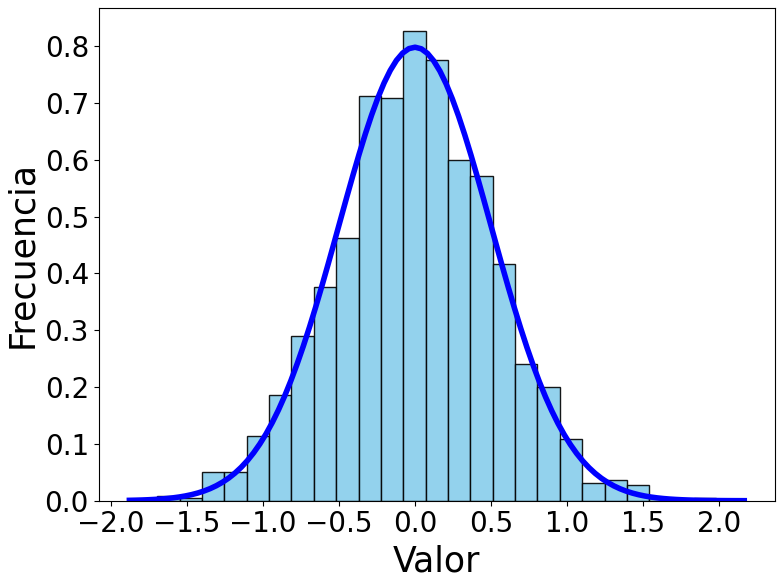
\includegraphics[width=\textwidth]{img/experiments/unimodal.png}
        \caption{Distribución unimodal.}\label{fig:unimodal}
    \end{subfigure}
    \hfill
    \begin{subfigure}[b]{0.43\textwidth}
        \centering
        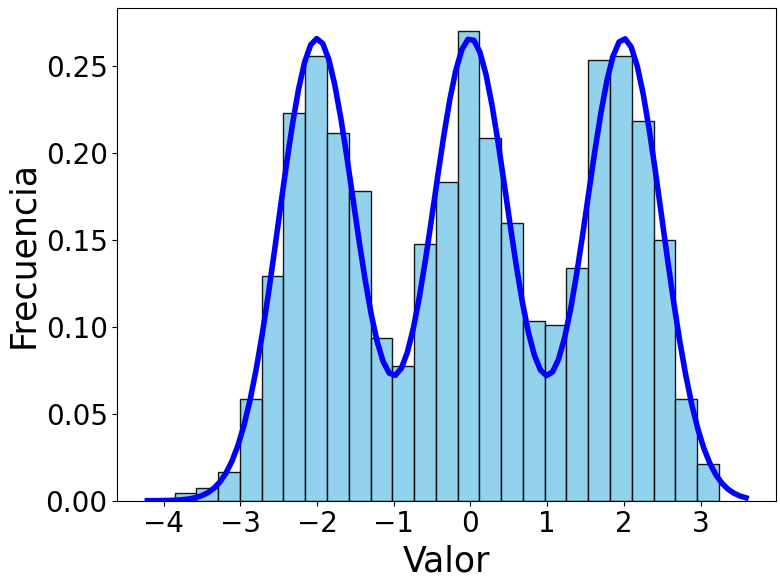
\includegraphics[width=\textwidth]{img/experiments/multimodal.png}
        \caption{Distribución multimodal con tres modas.}\label{fig:multimodal}
    \end{subfigure}
    \caption[Comparación de distribuciones unimodal y multimodal.]{Ejemplos de distribuciones unimodal y multimodal. La distribución unimodal muestra un único máximo, mientras que la distribución multimodal presenta tres máximos, cada uno correspondiente a una moda.}\label{fig:unimodal-multimodal}
\end{figure}

\subsection{Distribución Normal}
La distribución normal, o distribución de Gauss, es la distribución de probabilidad más estudiada y utilizada en el ámbito de la inferencia estadística~\cite{Bryc1995TheND}, dadas sus propiedades matemáticas, como su simetría, la concentración de probabilidades alrededor de la media y su relación con otras distribuciones.

\begin{definicion}[Distribución normal]
    Sea $X$ una variable aleatoria continua. Decimos que $X$ sigue una \emph{distribución normal} si su función de densidad $f_X$ viene dada por:

    \[ f_X(x) = \frac{1}{\sqrt{2\pi \sigma^2}} \cdot e^{-\frac{{(x - \mu)}^2}{2\sigma^2}}, \]

    donde $\mu, \sigma^2 \in \mathbb{R}$ denotan, respectivamente, la esperanza y varianza de la variable aleatoria $X$.

    Además, si $X$ sigue una distribución normal, lo denotaremos como $X \sim \mathcal{N}(\mu,\sigma^2)$. De igual modo, si $\mu = 0$ y $\sigma^2=1$, entonces diremos que la variable aleatoria $X \sim \mathcal{N}(0,1)$ sigue una \emph{distribución normal estándar}.
\end{definicion}

\begin{proposicion}
    Si $X \sim \mathcal{N}(\mu,\sigma^2)$, entonces la variable aleatoria $X$ satisface las siguientes propiedades:

    \begin{itemize}
        \item La distribución es simétrica respecto de su media $\mu$.
        \item La moda coincide con la media.
        \item $P[\mu - \sigma < X < \mu + \sigma] \approx 0,6826$.
        \item $P[\mu - 2\sigma < X < \mu + 2\sigma] \approx 0,9544$.
        \item $P[\mu - 3\sigma < X < \mu + 3\sigma] \approx 0,9974$.
        \item Si $a, b \in \mathbb{R}$, entonces $aX + b \sim \mathcal{N}(a\mu + b, a^2\sigma^2)$.
    \end{itemize}
\end{proposicion}

Como consecuencia de la primera propiedad de la proposición anterior, se pueden relacionar todas las variables aleatorias normales con la distribución $\mathcal{N}(0,1)$.

\begin{proposicion}
    Sea $X \sim \mathcal{N}(\mu,\sigma^2)$. Entonces
    
    \[ Z = \frac{X-\mu}{\sigma} \]

    es una variable aleatoria que sigue una distribución normal estándar $Z \sim\mathcal{N}(0,1)$.
\end{proposicion}

\begin{figure}[h]
    \centering
    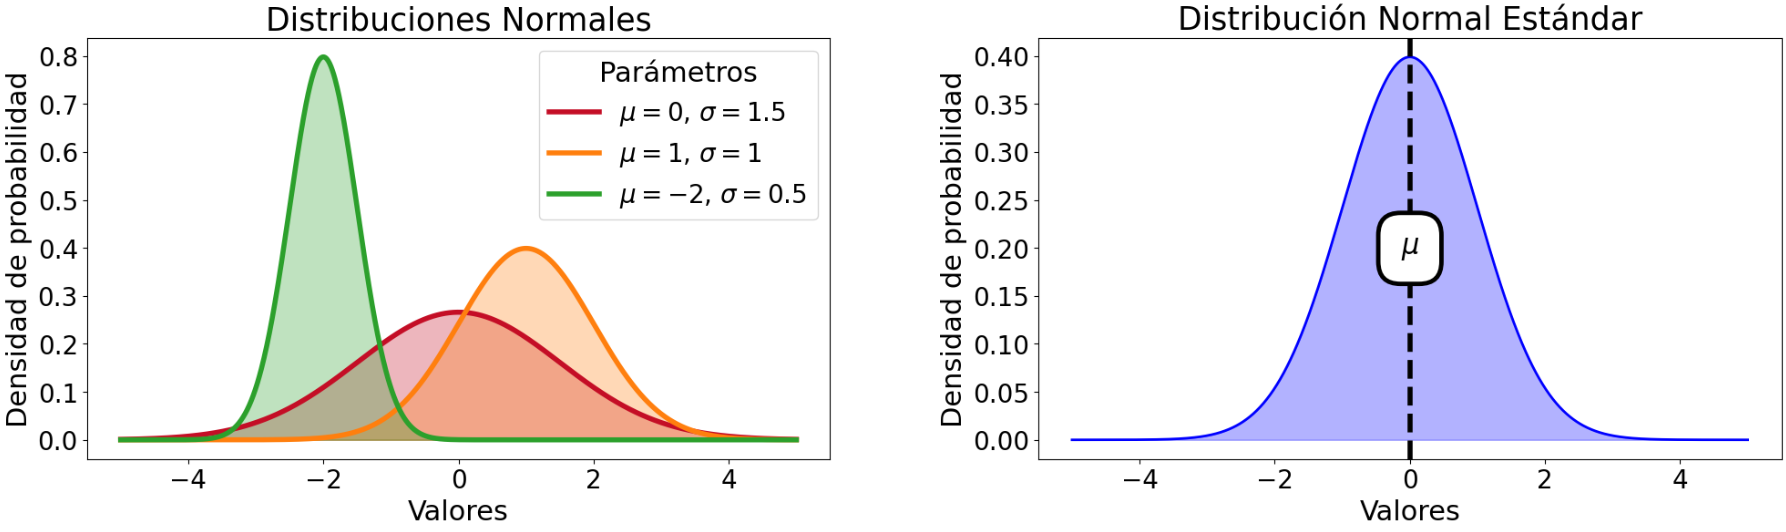
\includegraphics[width=0.9\textwidth]{img/distribuciones-normales.png}
    \caption[Ejemplos de distribuciones normales.] {Ejemplos de distribuciones normales. A la izquierda observamos distintas distribuciones normales, donde podemos notar como el parámetro $\mu$ determina el centro de la distribución y el parámetro $\sigma$ controla la dispersión de los datos. A medida que el parámetro $\sigma$ incrementa, la distribución se vuelve más dispersa y su altura máxima disminuye. A la derecha observamos una distribución normal estándar, donde se puede apreciar con claridad que la distribución es simétrica con respecto a $\mu$.}\label{fig:distribuciones-normales}
\end{figure}

\subsection{Distribución de Rademacher}\label{subsec:distribucion-rademacher}
La distribución de Rademacher es una distribución de probabilidad discreta que se utiliza ampliamente en la teoría del aprendizaje estadístico, particularmente en el análisis de la capacidad de generalización de los modelos.

\begin{definicion}[Distribución de Rademacher]
    Sea $X$ una variable aleatoria discreta. Decimos que $X$ sigue una \emph{distribución de Rademacher} si toma los valores $+1$ y $-1$ con igual probabilidad, es decir,

    \[
        P[X = 1] = P[X = -1] = \frac{1}{2}.
    \]

    En tal caso, denotamos esta variable como $X \sim \text{Rad}$.
\end{definicion}

\begin{proposicion}
    Si $X \sim \text{Rad}$, entonces $X$ es una variable aleatoria simétrica respecto al origen, con esperanza $\mathbb{E}[X] = 0$ y varianza $\text{Var}(X) = 1$.
\end{proposicion}

\begin{proposicion}
    Sean $X_1, \dots, X_n$ variables independientes con $X_i \sim \text{Rad}$. Entonces, para cualquier conjunto de constantes $a_1, \dots, a_n \in \mathbb{R}$, la variable

    \[
        S = \sum_{i=1}^n a_i X_i
    \]

    es una combinación lineal de variables de Rademacher con esperanza cero y varianza $\sum_{i=1}^n a_i^2$.
\end{proposicion}


\chapter{Descomposición en Valores Singulares y Pseudoinversa de una Matriz}\label{ch:descomposicion-valores-singulares-pseudoinversa}

En este capítulo presentaremos dos conceptos fundamentales de cara al desarrollo del trabajo: la descomposición en valores singulares (SVD) y la pseudoinversa de una matriz. En cuanto a las referencias utilizadas a lo largo de este capítulo, debemos destacar~\cite{Friedberg2014linear, Strang2023, Poole2011}. Estos libros nos han ayudado a presentar los conceptos básicos más importantes, así como las demostraciones de los resultados más relevantes del capítulo.

\section{Vectores y matrices}\label{sec:vectores-matrices}

En primer lugar, repasaremos la notación que utilizaremos para vectores y matrices, así como los principales tipos de matrices con las que trabajaremos. Además, recordaremos las condiciones bajo las cuales una matriz posee inversa.

Trabajaremos siempre con escalares reales y escribiremos los vectores de $\mathbb{R}^{n}$ como vectores columna en lugar de vectores fila. Es decir, si $v \in \mathbb{R}^{n}$, entonces

\[ 
    v = \begin{pmatrix} 
        v_{1} \\ 
        v_{2} \\ 
        \vdots \\
        v_{n}
    \end{pmatrix} = {(v_{1}, v_{2}, \ldots, v_{n})}^{T}, \quad \text{donde } v_i \in \mathbb{R} \ \ \forall i \in \{1, \ldots, n \}.
\]

También se recuerdan los conceptos de norma y ortonormalidad de vectores, que serán de gran utilidad en el desarrollo de resultados posteriores. De esta manera, dados dos vectores $u, v \in \mathbb{R}^{n}$, denotaremos por $u \cdot v$ su producto escalar usual y por $\| u \|$ la norma euclídea del vector $u$. Así, diremos que dos vectores son ortogonales si su producto escalar es igual a cero.

Denotaremos por $\mathcal{M}_{m \times n}(\mathbb{R})$ al espacio vectorial de las matrices de orden $m$ por $n$ con entradas en $\mathbb{R}$. A la matriz cuyas entradas son todas iguales a cero la llamaremos matriz cero y la denotaremos por $O$. Además, podemos formar una matriz a partir de vectores columna, utilizando la notación $V = [v_1, v_2, \ldots, v_n]$, donde $\{v_1, v_2, \ldots, v_n\}$ son los vectores columna que componen la matriz V.

\begin{definicion}
    La matriz \textbf{traspuesta} $A^{T}$ de una matriz $A \in \mathcal{M}_{m \times n}(\mathcal{R})$ es la matriz de tamaño $n \times m$ que se obtiene de la matriz $A$ al intercambiar las filas por las columnas, es decir, $(a^{T})_{ij} = a_{ji}$. Decimos que una matriz cuadrada $A$ es \textbf{simétrica} si cumple $A^{T} = A$ y decimos que es \textbf{ortogonal} si sus columnas están formadas por vectores ortonormales dos a dos.
\end{definicion}

Denotamos la \textbf{delta de Kronecker} $\delta_{ij}$ como la función dada por

\[
    \delta_{ij} =
    \begin{cases}
        1 & \text{si } i = j \leq r, \\
        0 & \text{si } i \neq j.
    \end{cases}
\]

De esta manera, la \textbf{matriz identidad} de tamaño $n \times n$ ($I_{n}$) viene dada por $(I_n)_{ij} = \delta_{ij}$.

\begin{definicion}
    Sea $A$ una matriz de tamaño $m \times n$. Se dice que $A$ es una matriz \textbf{escalonada} si es la matriz $O$, o bien satisface las tres condiciones siguientes:

    \begin{enumerate}
        \item El primer elemento no nulo de cada fila, si existe, es un $1$.
        \item El primer $1$ de la segunda y sucesivas filas está a la derecha del primer $1$ de la fila anterior.
        \item Si tiene filas nulas (compuestas únicamente por ceros), estas aparecen en la parte inferior de la matriz, justo debajo de las filas no nulas.
    \end{enumerate}

    Además, las operaciones elementales que se pueden realizar a una matriz para obtener su forma escalonada son las siguientes:

    \begin{itemize}
        \item Intercambiar dos filas (columnas).
        \item Multiplicar una fila (columna) por un múltiplo distinto de cero.
        \item Sumar un múltiplo de una fila (columna) a otra fila (columna).
    \end{itemize}
\end{definicion}

\begin{definicion}
    Sean $A$ y $B$ dos matrices de tamaño $m \times n$. Se dice que la matriz $A$ es \textbf{equivalente} por filas a la matriz $B$ (o simplemente equivalente) si $B$ se obtiene de $A$ por medio de la aplicación sucesiva de operaciones elementales.
\end{definicion}

\begin{definicion}
    Una matriz $A$ de tamaño $m \times n$ es \textbf{escalonada reducida} si es escalonada y además todo elemento en una columna que esté encima del primer uno de cualquier fila es cero.
\end{definicion}

\begin{ejemplo}
    Para matrices cuadradas de tamaño $2$, las posibles matrices escalonadas reducidas son las siguientes:

    \[
        \begin{pmatrix} 0 & 0 \\ 0 & 0 \end{pmatrix}, \quad
        \begin{pmatrix} 1 & 0 \\ 0 & 1 \end{pmatrix}, \quad
        \begin{pmatrix} 1 & $x$ \\ 0 & 0 \end{pmatrix} \quad y \quad
        \begin{pmatrix} 0 & 1 \\ 0 & 0
        \end{pmatrix},
    \]

    donde $x \in \mathbb{R}$ puede ser cualquier escalar.
\end{ejemplo}

Una vez introducidas las definiciones anteriores, disponemos de todas las herramientas necesarias para introducir el concepto de rango de una matriz.

\begin{definicion}[Rango de una matriz]
    Sea $A$ una matriz de tamaño $m \times n$. Se denomina \textbf{rango} de $A$ ($rang(A)$) al número de filas no nulas de la matriz en la forma escalonada reducida equivalente a $A$. De manera equivalente, el rango de una matriz se puede definir como la dimensión del espacio generado por sus vectores fila o columna. De esta manera, el rango de una matriz será igual al número máximo de vectores fila o columna que sean linealmente independientes entre sí.
\end{definicion}

El siguiente resultado nos recuerda cómo utilizar el rango para determinar si una matriz es invertible.

\begin{proposicion}
    Sea $A$ una matriz cuadrada de tamaño $n$, entonces equivalen:

    \begin{enumerate}
        \item $A$ es invertible.
        \item $A$ es equivalente a $I_n$.
        \item El rango de $A$ es $n$.
        \item $\det(A) \neq 0$. Además, si $A$ es invertible, entonces $\det(A^{-1})=\frac{1}{\det(A)}$.
    \end{enumerate}
\end{proposicion}

Finalmente, recordamos algunas de las propiedades de las matrices invertibles.

\begin{proposicion}
    Sean $A$ y $B$ matrices cuadradas e invertibles del mismo tamaño. Entonces se cumple:

    \begin{enumerate}
        \item $A^{-1}$ es invertible y ${(A^{-1})}^{-1} = A$ (la inversa de $A^{-1}$ es la propia matriz $A$).
        \item $A^{T}$ es invertible y ${(A^{T})}^{-1} = {(A^{-1})}^{T}$.
        \item La matriz $AB$ es invertible y ${(AB)}^{-1} = B^{-1}A^{-1}$.
    \end{enumerate}
\end{proposicion}

\begin{definicion}
    Sea $A$ una matriz cuadrada de tamaño $n$. Un vector no nulo $v \in \mathbb{R}^{n}$ se dice que es un \textbf{vector propio} (o autovector) de la matriz $A$ si $Av=\lambda v$ para algún escalar $\lambda \in \mathbb{R}$. Además, el escalar $\lambda$ se llama \textbf{valor propio} (o autovalor) de la matriz $A$ correspondiente al vector propio $v$. Recordemos que $\lambda$ es un valor propio de $A$ si, y solo si, $det(A-\lambda I_n)=0$.
\end{definicion}

Para cualquier matriz $A \in \mathcal{M}_{m \times n}(\mathbb{R})$, la matriz $A^{T}A$ es simétrica y, en consecuencia, es diagonalizable ortogonalmente (teorema espectral real~\cite{Blum2021}). Se comprueba de manera sencilla que todos los valores propios de la matriz $A^{T}A$ son no negativos.

\section{SVD y pseudoinversa}\label{sec:svd-pseudoinversa}

LLegados a este punto, ya podemos presentar los principales contenidos sobre matrices abordados en este trabajo: la descomposición en valores singulares y la pseudoinversa. Cabe destacar que estos resultados se enuncian para matrices con escalares en el cuerpo $\mathbb{R}$, aunque su generalización a otros cuerpos es posible.

\begin{definicion}
    Si $A$ es una matriz de tamaño $m \times n$, los \textbf{valores singulares} de $A$ son las raíces cuadradas (positivas) de los valores propios de la matriz $A^{T}A$, y se denotan mediante $\sigma_{1}, \sigma_{2}, \ldots, \sigma_{n}$. Además, es convencional ordenar los valores singulares de manera que $\sigma_{1} \geq \sigma_{2} \geq \cdots \geq \sigma_{n}$.
\end{definicion}


El siguiente resultado nos indica que toda matriz, independientemente de su estructura, puede ser factorizada como producto de tres matrices, dos de las cuales serán ortogonales.

\begin{teorema}[Descomposición en valores singulares]
    Sea $A \in \mathcal{M}_{m \times n}(\mathbb{R})$ una matriz cuyo rango es $r$ y con valores singulares positivos $\sigma_{1} \geq \sigma_{2} \geq \cdots \geq \sigma_{r}$, y sea $\Sigma$ la matriz de tamaño $m \times n$ definida por 

    \[
        \Sigma_{ij} =
        \begin{cases}
            \sigma_i & \text{si } i = j \leq r, \\
            0 & \text{en otro caso.}
        \end{cases}
    \]

    Entonces existen matrices ortogonales $U$ y $V$ de tamaño $m\times m$ y $n\times n$, respectivamente, de manera que

    \[
        A = U \Sigma V^{T}.
    \]

    A esta factorización la llamaremos \textbf{descomposición en valores singulares (SVD)} de $A$.
\end{teorema}

\begin{proof}
    La demostración se fundamenta en la construcción directa de las matrices $V$ y $U$, verificando posteriormente que se satisface el resultado buscado.

    Para construir la matriz ortogonal $V$, basta tomar una base ortonormal $\{v_1, v_2, \ldots, v_n \}$ de $\mathbb{R}^{n}$ formada por vectores asociados a los valores propios $\{\lambda_1, \lambda_2, \ldots, \lambda_n\}$ de la matriz simétrica y cuadrada $A^{T}A$ de tamaño $n$. Entonces, se tiene que $V = [v_1, v_2, \ldots, v_n]$ es una matriz ortogonal y cuadrada de tamaño $n$.

    Para construir la matriz ortogonal $U$, primero notemos que $\{Av_1, Av_2, \ldots, Av_n \}$ es un conjunto ortogonal de vectores de $\mathbb{R}^{m}$. En efecto, para $i \neq j$, se cumple

    \[ (Av_i)\cdot(Av_j) = (Av_i)^{T}Av_j=v_{i}^{T}A^{T}Av_j = v_{i}^{T}\lambda_j v_j=\lambda_j(v_i \cdot v_j) = 0,\]

    dado que los vectores propios $v_i$ son ortogonales. Recordamos ahora que los valores singulares satisfacen $\sigma_i = ||Av_i||$ y que los primeros $r$ valores singulares son distintos de cero. Por tanto, podemos normalizar $Av_1, \ldots, Av_r$ de la siguiente forma:

    \begin{equation}
        u_i = \frac{1}{\sigma_i} A v_i \quad \text{para } i = 1, \ldots, r.
        \label{eq:singulares1}
    \end{equation}
    

    Esto garantiza que $\{ u_1, \ldots, u_r\}$ es un conjunto ortonormal de $\mathbb{R}^{m}$, pero si $r < m$ no será una base para $\mathbb{R}^{m}$. En este caso, se extiende el conjunto $\{u_1, \ldots, u_r \}$ a una base ortonormal $\{u_1, \ldots, u_m \}$ para $\mathbb{R}^{m}$. En consecuencia, la matriz $U$ es ortogonal. Ahora, falta comprobar que, con la construcción realizada, se satisface el resultado $A = U \Sigma V^{T}$. Dado que $V^{T} = V^{-1}$ (al ser la matriz $V$ ortogonal), esto equivale a demostrar que $AV = U\Sigma$.

    En primer lugar, sabemos, a partir de la ecuación~\eqref{eq:singulares1}, que $Av_i=\sigma_i u_i$ para $i=1, \ldots, r$ y que $||A v_i|| = \sigma_i = 0$ para $i=r+1, \ldots,n$. En consecuencia, $Av_i = 0$ para $i=r+1, \ldots,n$. Por tanto, 

    \begin{align*}
        A V &= A \begin{bmatrix} \mathbf{v}_1 & \cdots & \mathbf{v}_n \end{bmatrix} \\
            &= \begin{bmatrix} A \mathbf{v}_1 & \cdots & A \mathbf{v}_n \end{bmatrix} \\
            &= \begin{bmatrix} A \mathbf{v}_1 & \cdots & A \mathbf{v}_r & 0 & \cdots & 0 \end{bmatrix} \\
            &= \begin{bmatrix} \sigma_1 \mathbf{u}_1 & \cdots & \sigma_r \mathbf{u}_r & 0 & \cdots & 0 \end{bmatrix} \\
            &= \begin{bmatrix} \mathbf{u}_1 & \cdots & \mathbf{u}_m \end{bmatrix}
               \begin{bmatrix} 
                   \sigma_1 & \cdots & 0 & O \\
                   \vdots & \ddots & \vdots & O \\
                   0 & \cdots & \sigma_r & O \\
                   O & O & O & O
               \end{bmatrix} \\
            &= U \Sigma,
    \end{align*}

    quedando probada la igualdad $AV = U \Sigma$.
\end{proof}

El siguiente resultado generaliza el concepto de matriz inversa cuando la matriz no es cuadrada.
\begin{definicion}[Pseudoinversa]
    Sea $A \in \mathcal{M}_{m \times n}(\mathbb{R})$ con $m > n$ y cuyas columnas son linealmente independientes. Se define la \textbf{pseudoinversa} \emph{(o inversa de Moore-Penrose)} de la matriz $A$ como la matriz $A^{\dagger}$ dada por

    \[ A^{\dagger} = {(A^{T}A)}^{-1}A^{T}, \]

    donde se puede comprobar que $A^{\dagger} \in \mathcal{M}_{n \times m}(\mathbb{R})$.
\end{definicion}

No obstante, dado que toda matriz se puede factorizar en su descomposición en valores singulares, podemos definir la pseudoinversa de una matriz a partir de dicha factorización.
\begin{definicion}
    Sea $A$ una matriz de tamaño $m \times n$ de rango $r$ con descomposición en valores singulares $A = U \Sigma V^{T}$ y con valores singulares distintos de cero $\sigma_{1} \geq \sigma_{2} \geq \cdots \geq \sigma_{r}$. Sea $\Sigma^{\dagger}$ la matriz de tamaño $n \times m$ definida por

    \[
        \Sigma^{\dagger}_{ij} =
        \begin{cases}
            \frac{1}{\sigma_i} & \text{si } i = j \leq r, \\
            0 & \text{en otro caso.}
        \end{cases}
    \]

    Entonces la factorización $A^{\dagger} = V \Sigma^{\dagger} U^{T}$ es una descomposición en valores singulares de $A^{\dagger}$, donde $\Sigma^{\dagger}$ es la pseudoinversa de $\Sigma$. Además, $A^{\dagger}$ es la pseudoinversa de $A$.
\end{definicion}

Presentamos una forma análoga de definir la pseudoinversa de una matriz, basándose en las propiedades que debe cumplir la pseudoinversa, que serán de gran utilidad en el desarrollo del trabajo.
\begin{definicion}[Condiciones de Moore-Penrose]
    Sea $A \in \mathcal{M}_{m \times n}(\mathbb{R})$ la pseudoinversa de $A$, $A^{\dagger} \in \mathcal{M}_{n \times m}(\mathbb{R})$, es la única matriz que satisface las siguientes propiedades, conocidas como las \textbf{condiciones de Moore-Penrose}:

    \begin{enumerate}
        \item $A A^{\dagger} A = A$.
        \item $A^{\dagger} A A^{\dagger} = A^{\dagger}$.
        \item ${(A A^{\dagger})}^{T}$ y ${(A^{\dagger} A)}^{T}$ son simétricas.
    \end{enumerate}

    En particular, se tiene que $AA^{\dagger}$ y $A^{\dagger}A$ son proyecciones ortogonales sobre $Im(A)$ y ${Im(A)}^{T}$ respectivamente. Además, si $A$ es de rango completo, es decir, $rango(A) = r  = \min\{m, n\}$, entonces $A^{\dagger}$ puede expresarse de forma sencilla como sigue:

    \begin{itemize}
        \item Si $r = m = n$, entonces la matriz $A$ es invertible y $A^{\dagger} = A^{-1}$.
        \item Si $r = m < n$, entonces $A$ tiene filas linealmente independientes (la aplicación lineal asociada a $A$ es sobreyectiva y $AA^{T}$ es invertible) y $A^{\dagger} = A^{T}{(AA^{T})}^{-1}$.
        \item Si $r = n < m$, entonces $A$ tiene columnas linealmente independientes (la aplicación lineal asociada a $A$ es inyectiva y $A^{T}A$ es invertible) y $A^{\dagger} = {(A^{T}A)}^{-1} A^{T}$.
    \end{itemize}
\end{definicion}

A continuación, se presentan dos propiedades de la pseudoinversa que son fundamentales para comprender la estructura de la solución de sistemas lineales.

\begin{lema}\label{lema:propiedades-pseudoinversa}
    Para una matriz $A \in \mathcal{M}_{m \times n}(\mathbb{R})$, se verifica:

    \begin{enumerate}
        \item $\operatorname{Im}(I-A^{\dagger}A) = \ker(A)$.
        \item $\ker(A^{\dagger}) = \ker(A^{T})$.
    \end{enumerate}

    Donde $\operatorname{Im(A)}$ y $\ker(A)$ denotan, respectivamente, la imagen y el núcleo de la aplicación lineal asociada a la matriz $A$.
\end{lema}

Finalmente, la solución de norma mínima para un problema de mínimos cuadrados puede definirse mediante la pseudoinversa de una matriz, como se establece en el siguiente teorema. Más adelante, este resultado será de gran utilidad para obtener la mejor aproximación en problemas de regresión.

\begin{teorema}
    El problema de mínimos cuadrados $A\mathbf{x}=\mathbf{b}$, con $A \in \mathcal{M}_{m \times n}(\mathbb{R})$, $\mathbf{x} \in \mathbb{R}^{n}$ y $\mathbf{b} \in \mathbb{R}^{m}$, tiene una solución única $\bar{x}$ de mínimos cuadrados con norma mínima dada por

    \[ \bar{\mathbf{x}} = A^{\dagger}\mathbf{b}. \]
\end{teorema}

\begin{proof}
    Sea $A \in \mathcal{M}_{m \times n}(\mathbb{R})$ con $rang(A) = r$ y sea $U\Sigma V^{T}$ su descomposición en valores singulares. De este modo, se tiene que $A^{\dagger} = V \Sigma^{\dagger} U^{T}$. Sean $\mathbf{y}=V^{T}\mathbf{x}$ y $\mathbf{c}=U^{T}\mathbf{b}$, expresados de la siguiente forma

    \[
        \mathbf{y} = \begin{bmatrix} \mathbf{y}_1 \\ \mathbf{y}_2 \end{bmatrix}, \quad 
        \mathbf{c} = \begin{bmatrix} \mathbf{c}_1 \\ \mathbf{c}_2 \end{bmatrix},
    \]

    donde $\mathbf{y_1}, \mathbf{c_1} \in \mathbb{R}^{r}$.

    Se busca minimizar $\|\mathbf{b} - A \mathbf{x}\|$ o, de manera equivalente, $\|\mathbf{b} - A \mathbf{x}\|^2$. Usando que $U^T$ es ortogonal (dado que $U$ es ortogonal), se tiene  

    \[
        \|\mathbf{b} - A \mathbf{x}\|^2 = \| U^T (\mathbf{b} - A \mathbf{x}) \|^2 = \| U^T (\mathbf{b} - U \Sigma V^T \mathbf{x}) \|^2 = \| U^T \mathbf{b} - U^T U \Sigma V^T \mathbf{x} \|^2
    \]

    \[
        = \|\mathbf{c} - \Sigma \mathbf{y}\|^2 = \left\| \begin{bmatrix} \mathbf{c}_1 \\ \mathbf{c}_2 \end{bmatrix} - \begin{bmatrix} D & O \\ O & O \end{bmatrix} \begin{bmatrix} \mathbf{y}_1 \\ \mathbf{y}_2 \end{bmatrix} \right\|^2 = \left\| \begin{bmatrix} \mathbf{c}_1 - D \mathbf{y}_1 \\ \mathbf{c}_2 \end{bmatrix} \right\|^2.
    \]

    Dado que sólo disponemos de control sobre $\mathbf{y}_1$, el valor mínimo ocurre cuando $\mathbf{c}_1 - D \mathbf{y}_1 = 0$ o, de manera equivalente, cuando $\mathbf{y}_1 = D^{-1} \mathbf{c}_1$. De modo que todas las soluciones $\mathbf{x}$ de mínimos cuadrados son de la forma  

    \[
        \mathbf{x} = V \mathbf{y} = V \begin{bmatrix} D^{-1} \mathbf{c}_1 \\ \mathbf{y}_2 \end{bmatrix}.
    \]

    Definimos $\bar{\mathbf{x}} = V \bar{\mathbf{y}} = V \begin{bmatrix} D^{-1} \mathbf{c}_1 \\ 0 \end{bmatrix}$ y afirmamos que $\bar{\mathbf{x}}$ es la solución de mínimos cuadrados de norma mínima. Para demostrarlo, supongamos que $\mathbf{x}^{\prime}=V\mathbf{y}^{\prime} = V \begin{bmatrix} D^{-1} \mathbf{c}_1 \\ y_2 \end{bmatrix}$ es otra solución diferente al problema de mínimos cuadrados (por tanto, $\mathbf{y}_2 \neq 0$). Entonces, se verifica

    \[ \| \bar{\mathbf{x}} \| = \| V\bar{\mathbf{y}} \| = \| \bar{\mathbf{y}} \| < \| {\mathbf{y}^{\prime}} \| = \| V\mathbf{y}^{\prime} \| = \| \mathbf{x}^{\prime} \|,\]

    como se quería probar. Por último, falta demostrar que $\bar{\mathbf{x}}$ es igual a $A^{\dagger}\mathbf{b}$. Para ello, basta calcular

    \[ \bar{\mathbf{x}} = V\bar{\mathbf{y}} = V \begin{bmatrix} D^{-1} \mathbf{c}_1 \\ 0 \end{bmatrix} = V \begin{bmatrix} D^{-1} & O \\ O & O \end{bmatrix} \begin{bmatrix} \mathbf{c}_1 \\ \mathbf{c}_2 \end{bmatrix} = V \Sigma^{\dagger} \mathbf{c} = V \Sigma^{\dagger} U^{T} \mathbf{b} = A^{\dagger}\mathbf{b}.\]

    
\end{proof}

% \chapter{Aproximación lineal}\label{ch:capitulo-aproximacion-lineal}

\endinput
% !TeX root = ../tfg.tex
% !TeX encoding = utf8

\chapter{Aprendizaje Automático y Aprendizaje Profundo}\label{ch:capitulo-aprendizaje-automatico-y-profundo}

\section{Fundamentos}\label{sec:fundamentos-aprendizaje-automatico-y-aprendizaje-profundo}
El aprendizaje automático o \emph{machine learning} (ML) (\cite{Bishop2006},~\cite{Murphy2022} y~\cite{Murphy2023}) es una rama de la inteligencia artificial que, mediante el uso de datos y algoritmos de aprendizaje, proporciona a las máquinas la capacidad de aprender de manera automática de los datos. En otras palabras, el aprendizaje automático se encarga de utilizar un conjunto de observaciones para descubrir un proceso subyacente en los mismos (\cite{Mostafa2012}), con el objetivo de imitar el comportamiento humano, identificando patrones y relaciones en los datos.\newline

En términos generales, el aprendizaje automático se divide en tres tipos: el aprendizaje supervisado, que actúa sobre datos etiquetados (cada ejemplo de entrada se encuentra asociado a una salida conocida), el aprendizaje no supervisado, que trabaja sobre datos no etiquetados, donde es el propio sistema el que debe ser capaz de reconocer los patrones subyacentes de los datos mediante el uso exclusivo de los ejemplos de entrada, y el aprendizaje por refuerzo, que actúa en un entorno de ensayo-error, donde el modelo aprende a través de recompensas y penalizaciones que se le otorgan a medida que realiza las acciones. Para nuestro trabajo, nos limitaremos a trabajar con el \emph{aprendizaje supervisado}.\newline

\begin{figure}[h]
    \centering
    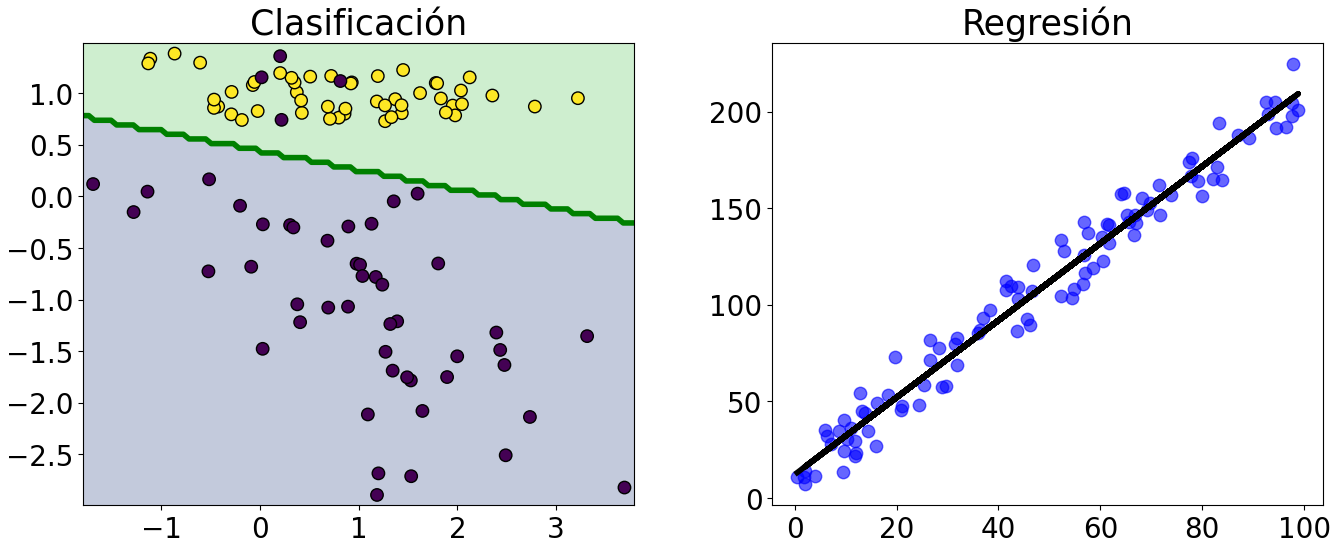
\includegraphics[width=0.8\linewidth]{img/clasi-regresion.png}
    \caption[Ejemplos de problemas de clasificación y regresión.]{Ejemplos de problemas de clasificación y regresión. A la izquierda, se muestra un problema de clasificación binario, donde se busca encontrar el hiperplano (línea verde) que separe ambos conjuntos de datos etiquetados. A la derecha, se muestra un problema de regresión, donde se busca encontrar la mejor aproximación (línea negra) al conjunto de datos. Imagen original del autor.}\label{fig:clasi-regresion}
\end{figure}

Dentro del marco del aprendizaje supervisado, donde el principal objetivo del modelo es aprender a predecir la salida correcta para nuevos ejemplos no conocidos, basándose en las relaciones y patrones extraídos al trabajar con los datos etiquetados, podemos dividir los problemas en dos categorías principales: problemas de clasificación en los que se asigna una salida o clase (discreta) a cada entrada y problemas de regresión en los que se predice un valor continuo para cada entrada (véase~\autoref{fig:clasi-regresion}). De cara al desarrollo de nuestro trabajo, abordaremos ambos tipos de problemas. En particular, en los problemas de clasificación nos centraremos en la clasificación de imágenes.\newline

El aprendizaje profundo o \emph{deep learning} (DL) (\cite{Bishop2023},~\cite{Prince2023} y~\cite{LeCun2015}) representa un área del aprendizaje automático que utiliza redes neuronales artificiales, inspiradas en la estructura y función del cerebro humano, con múltiples capas, conocidas como redes neuronales profundas (\cite{Goodfellow2016} y~\cite{Schmidhuber2015}), con el propósito de identificar y modelar patrones complejos y extraer representaciones jerárquicas en grandes volúmenes de datos.\newline

\section{Redes neuronales artificiales}\label{sec:redes-neuronales-artificiales}

Una red neuronal artificial o \emph{artificial neural network} (ANN) (\cite{Bishop1995},~\cite{Ripley1996}) es un modelo de aprendizaje automático que toma decisiones de manera similar al funcionamiento del cerebro humano, a partir de las interconexiones que presentan las neuronas biológicas, que se organizan en diferentes capas interconectadas. Estas conexiones simulan las interacciones entre las neuronas biológicas, permitiendo que la red procese información y aprenda de manera similar al propio cerebro humano.\newline

De manera similar al cerebro humano, una red neuronal artificial está formada por neuronas artificiales (véase~\autoref{fig:neuronasbioyartificial}), también llamadas unidades. Estas unidades se agrupan en diferentes capas formando la arquitectura global de la red neuronal. Cada capa puede contener un número variable de unidades, lo que permite adaptar la red a la complejidad del problema a resolver.\newline

\begin{figure}[h]
    \centering
    \subfloat{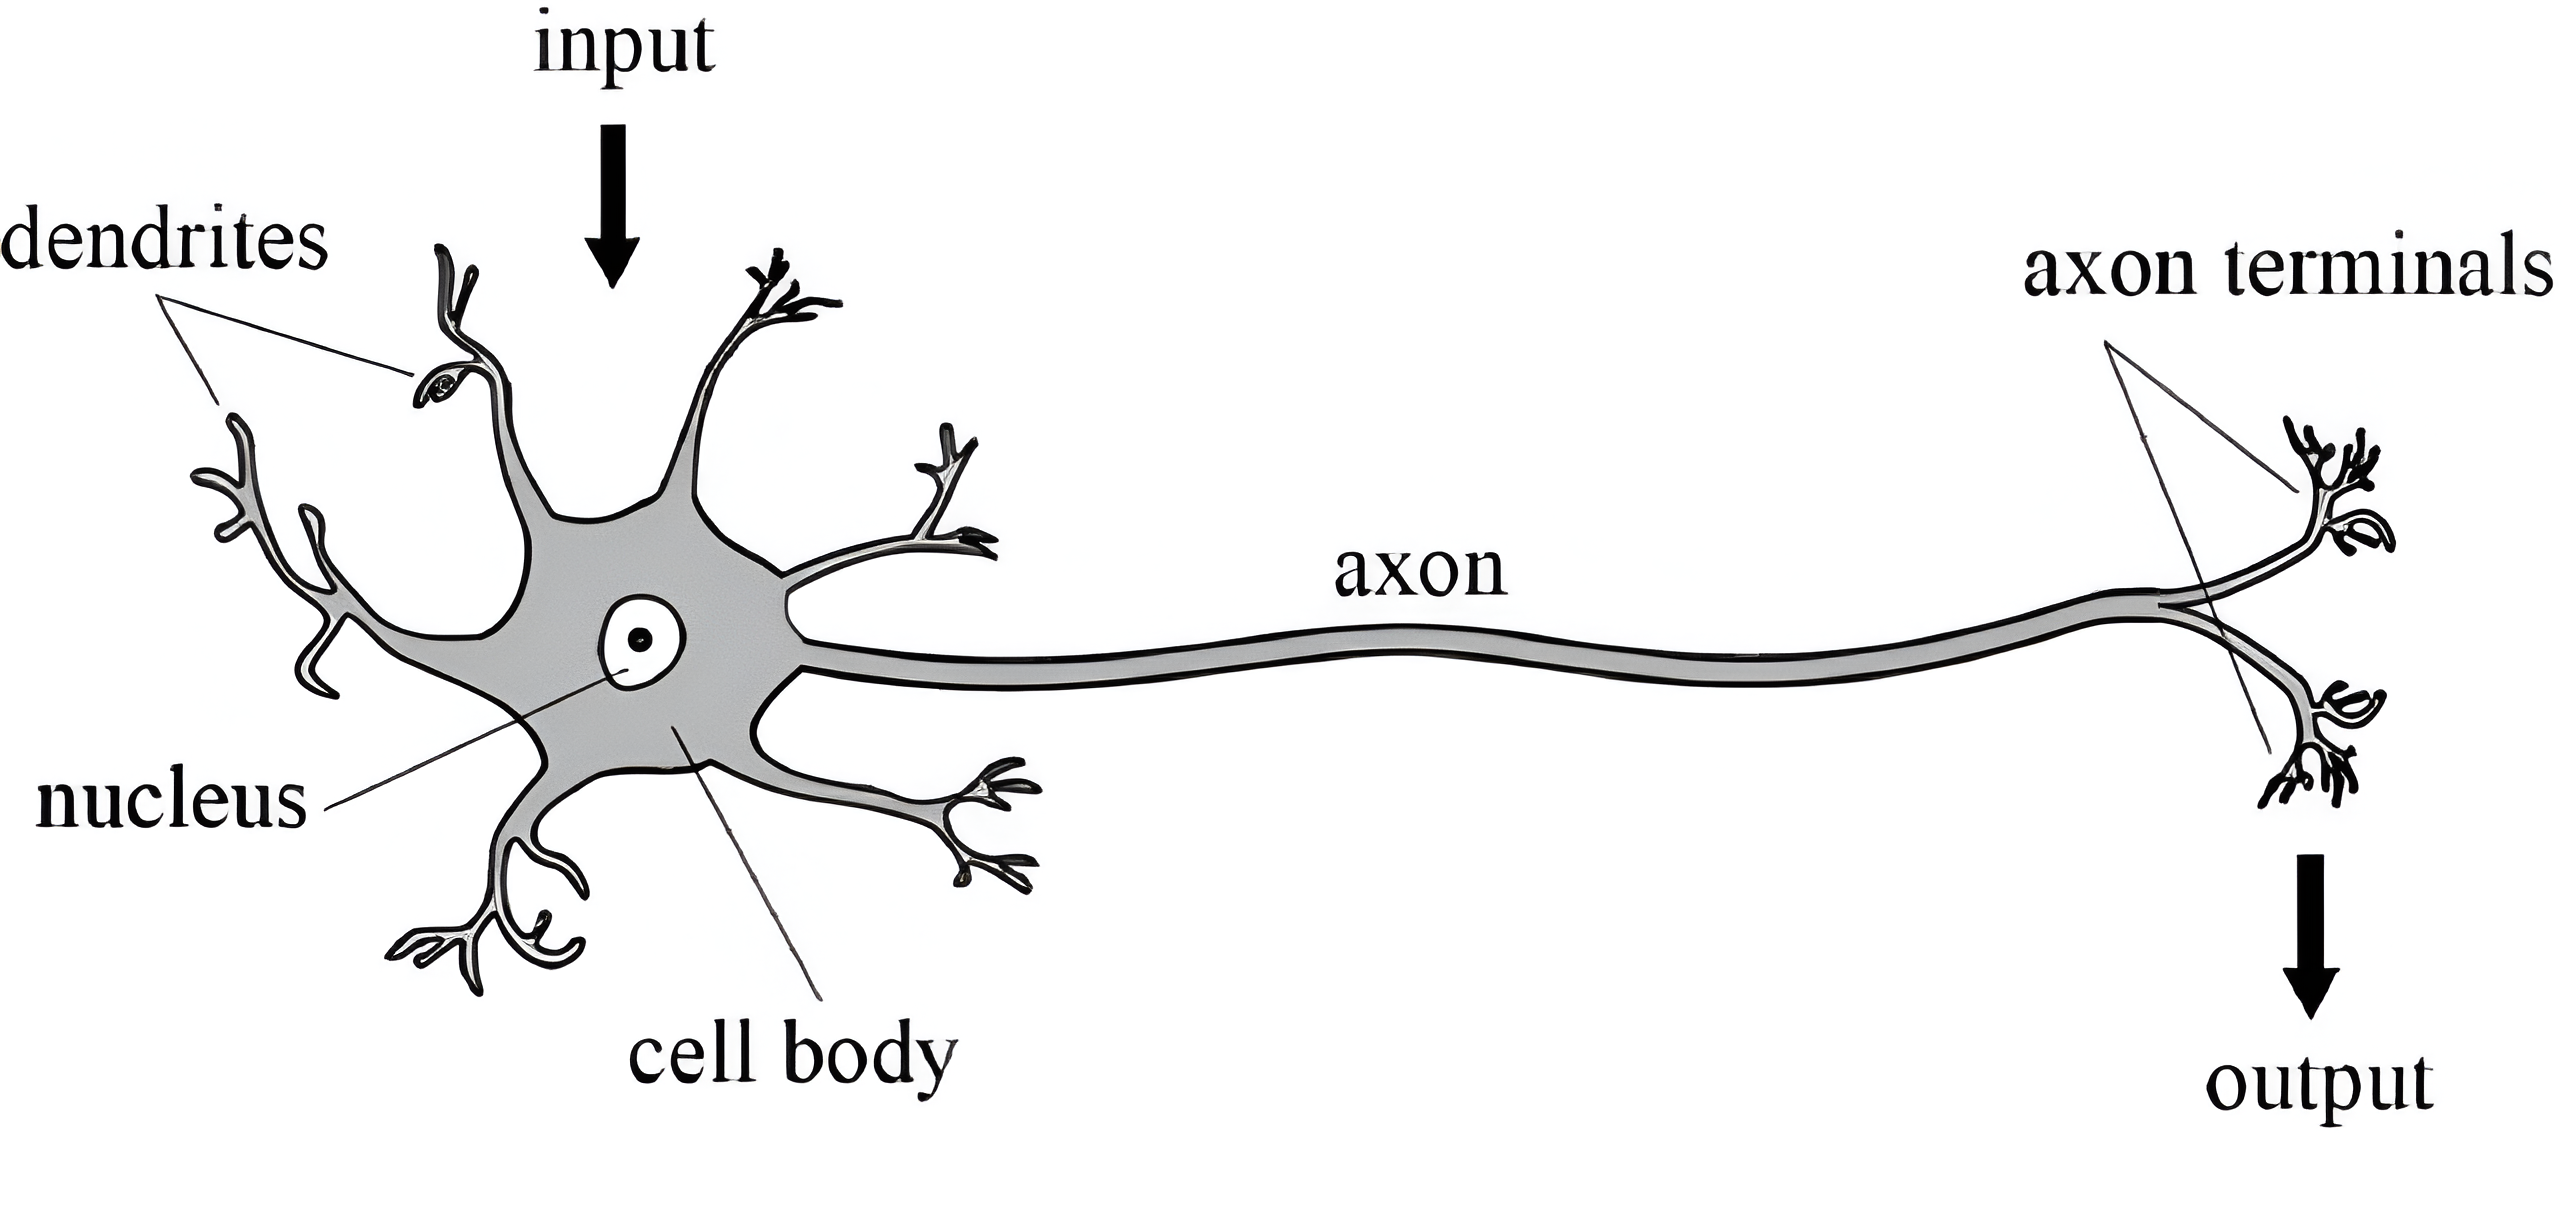
\includegraphics[width=0.45\textwidth]{img/biological-neuron.png}}
    \hfill
    \subfloat{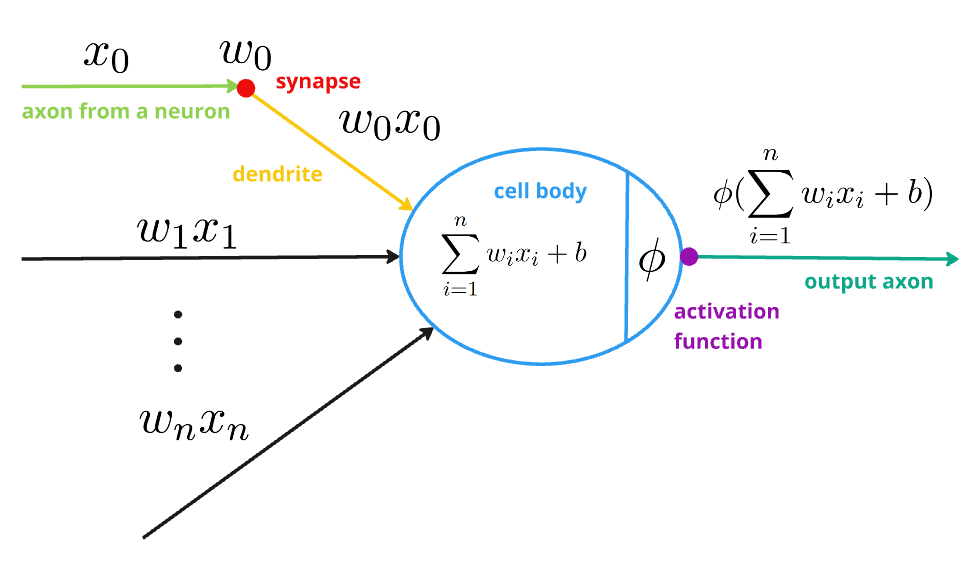
\includegraphics[width=0.45\textwidth]{img/artificial-neuron.png}}
    \caption[Ejemplos de neurona biológica~\cite{Neves2018} y neurona artificial (basada en~\cite{Li2024}).]{Ejemplos de una neurona biológica~\cite{Neves2018} (izquierda) y una neurona artificial (derecha) basada en~\cite{Li2024}.}\label{fig:neuronasbioyartificial}
\end{figure}

A alto nivel, el funcionamiento de una red neuronal artificial se divide en, al menos, tres capas principales, constituidas por una capa de entrada, una capa oculta y una capa de salida. En la primera capa o capa de entrada, la información del mundo exterior entra en la red neuronal. Dicha información es procesada y propagada al resto de capas mediante un proceso conocido como propagación hacia delante o \emph{forward propagation}, permitiendo que la información fluya desde la capa de entrada hacia las capas sucesivas.\newline

En la capa oculta o capa de procesamiento, las unidades reciben las salidas de la capa anterior y se encargan de procesar la información mediante conexiones ponderadas (llamadas pesos) y funciones de activación (encargadas de introducir no linealidad en el modelo, permitiendo que la red aprenda y represente relaciones complejas entre las entradas y las salidas), extrayendo características y patrones relevantes de los datos. Los pesos obtenidos controlan la influencia que cada neurona de la capa anterior tiene sobre la neurona actual. Las redes neuronales artificiales pueden tener una gran cantidad de capas ocultas, lo que permite un procesamiento más profundo y detallado de la información. Cada capa oculta analiza la salida de la capa anterior, la procesa aún más y la pasa a la siguiente capa, de modo que, a medida que se avanza por la red, se generan representaciones internas cada vez más abstractas de la entrada original.\newline

Finalmente, en la última capa o capa de salida, la red produce el resultado final en función del problema que se trate y de la predicción calculada haciendo uso de los pesos ajustados en las capas ocultas. La naturaleza de la salida varía según el tipo de tarea que se realice: en un problema de clasificación, la salida es un valor discreto que indica la clase a la que pertenece la entrada, mientras que en un problema de regresión, la salida es un valor continuo que representa una predicción numérica. Por tanto, esta capa es la que traduce la información procesada por la red en un resultado interpretable y acorde con el objetivo del problema.\newline

Por tanto, el proceso de entrenamiento de una red neuronal artificial es un proceso iterativo en el que la red ajusta sus pesos para aprender a realizar tareas específicas. Para llevar a cabo este proceso, es fundamental un conjunto de datos o ejemplos de entrenamiento que sea lo suficientemente representativo, ya que de este conjunto se extraerán los patrones relevantes que la red necesitará aprender.\newline

\subsection{Redes neuronales convolucionales}\label{subsec:redes-neuronales-convolucionales}

Las redes neuronales convolucionales o \emph{convolutional neural networks} (CNN) (\cite{LeCun1989}, \cite{LeCun1998}) son un tipo especial de red neuronal artificial que se utiliza principalmente en procesamiento de imágenes, reconocimiento visual y tareas relacionadas con datos que tienen una estructura de rejilla (matriz multidimensional), como imágenes, vídeos o señales de audio. Una de las características más destacadas de las redes neuronales convolucionales es su capacidad para realizar la extracción automática y jerárquica de características de los datos de entrada, lo que las hace especialmente poderosas para tareas que requieren reconocer patrones complejos en los datos.\newline

Esta capacidad de aprendizaje jerárquico de características es una de las principales razones por las que las CNN son tan eficaces, ya que permiten a la red identificar patrones relevantes sin necesidad de intervención humana para diseñar características específicas, lo que las vuelve especialmente interesantes en áreas como la visión por computador, donde han impulsado avances significativos en aplicaciones como el reconocimiento de imágenes, la segmentación semántica y la detección de objetos, entre otras.\newline

Las redes neuronales convolucionales incluyen varias capas especializadas que las distinguen de las redes neuronales artificiales tradicionales: las capas de convolución, encargadas de la extracción de características de la entrada; las capas de agrupación o \emph{pooling}, responsables de la reducción de la dimensionalidad de la entrada sin perder las características importantes y las capas totalmente conectadas o \emph{fully connected}, que se encuentran en la parte final de la red y que permiten combinar de manera efectiva las características extraídas por las capas anteriores para realizar la predicción final (véase~\autoref{fig:cnn}). Estas capas operan de manera conjunta, transformando la entrada y extrayendo progresivamente las características más relevantes, las cuales se van refinando y volviéndose más abstractas conforme se avanza por la red.\newline

\begin{figure}[h]
    \centering
    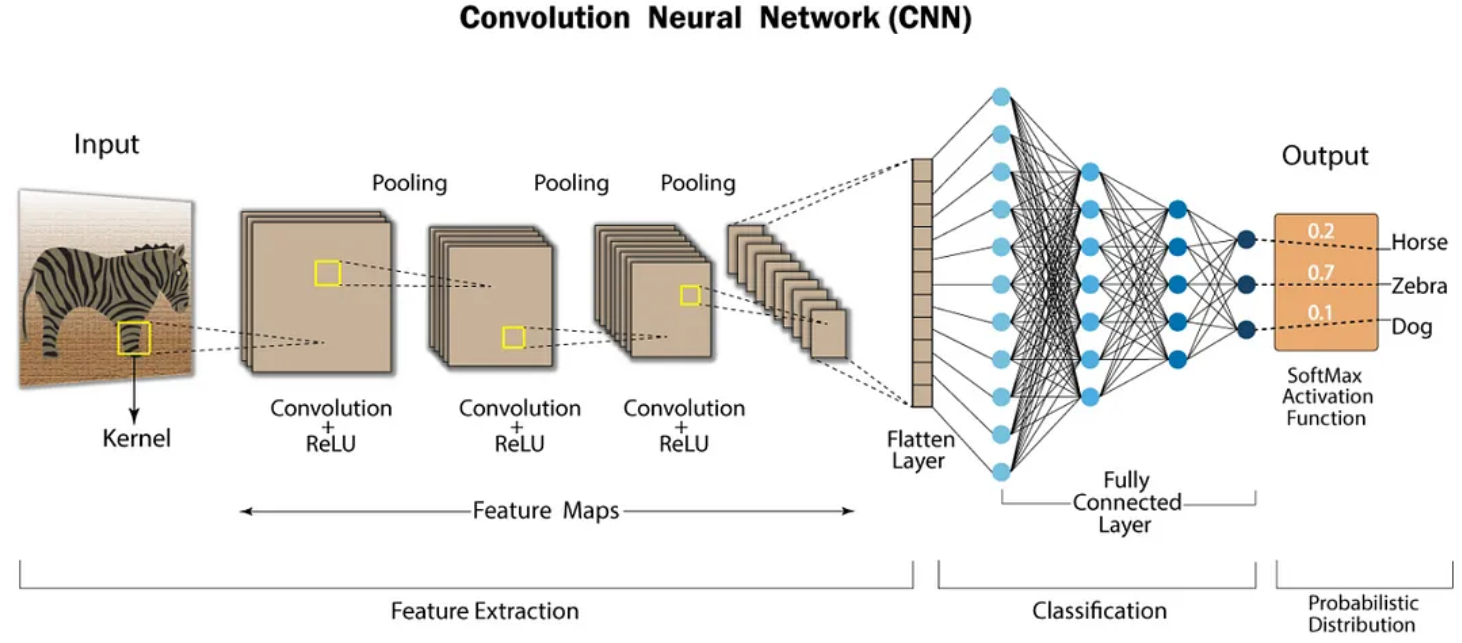
\includegraphics[width=0.8\linewidth]{img/cnn.png}
    \caption[Ejemplo de CNN utilizada para clasificación de imágenes~\cite{CNNSwapna}.]{Ejemplo de CNN utilizada para clasificación de imágenes~\cite{CNNSwapna}. La entrada a la red es una imagen en formato RGB. La extracción de características se realiza mediante varias capas convolucionales, seguidas de funciones de activación y capas de pooling, las cuales ayudan a reducir la dimensionalidad. Posteriormente, las características extraídas se aplanan (\textit{flattening}) y se envían a las capas totalmente conectadas. Finalmente, la salida pasa por una función de activación, en este caso softmax, que genera una distribución de probabilidad sobre las posibles clases de salida.}\label{fig:cnn}
\end{figure}

A continuación se describen las principales capas que conforman una red neuronal convolucional. Se incluyen tanto las capas exclusivas de este tipo de red como aquellas que comparte con las redes neuronales tradicionales:


\subsubsection{Capa de convolución}

La capa convolucional es un componente fundamental y exclusivo de las CNN, diseñada para extraer características locales de datos estructurados en forma de matrices multidimensionales. Su funcionamiento se basa en utilizar matrices de valores, conocidas como filtros o \emph{kernels}, que se deslizan sobre la entrada aplicando la operación matemática de convolución.\newline

La convolución es una operación lineal que consiste en desplazar un filtro sobre la entrada, realizando en cada posición una multiplicación elemento a elemento entre los valores del filtro y los de la entrada (diferente de una multiplicación matricial convencional). Posteriormente, se suman estos productos para obtener un único valor de salida. Este proceso se repite hasta deslizar el filtro a lo largo de toda la entrada, obteniendo una nueva matriz denominada mapa de características.\newline

Los valores de los filtros actúan como los pesos que la propia red aprende y optimiza de forma iterativa para maximizar la extracción de características relevantes de la entrada. Además, el número de filtros aplicados sobre cada entrada influye directamente en el mapa de características de salida resultante. Así, a mayor cantidad de filtros, la profundidad del mapa de características resultantes también es mayor.\newline

\begin{figure}[h]
    \centering
    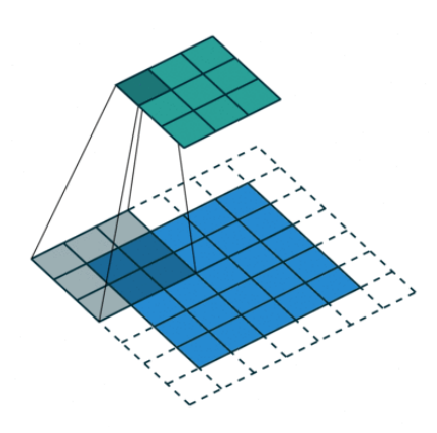
\includegraphics[width=0.5\linewidth]{img/convolucion.png}
    \caption[Ejemplo de convolución con padding~\cite{Saha2018}.]{Ejemplo de convolución con padding~\cite{Saha2018}. El color azul hace referencia a la entrada, mientras que el color verde denota el resultado de la convolución. En particular, el color verde oscuro destaca el resultado de la convolución que se realiza sobre la zona grisácea de la imagen, utilizando, en este caso, un filtro de tamaño 3x3. Por otra parte, las cuadrículas punteadas hacen referencia al padding agregado.}\label{fig:convolucion}
\end{figure}

Como se puede observar en la~\autoref{fig:convolucion}, la propia naturaleza de la operación de convolución modifica la dimensionalidad de la entrada. Sin embargo, esto no siempre es deseable, ya que en determinadas ocasiones preferiremos mantener la dimensión original de la entrada. Para solucionar este problema, se introduce el concepto de relleno o \emph{padding}, consistente en agregar información adicional alrededor de la entrada, con el fin de preservar su dimensionalidad.\newline

Por otra parte, la elección de la siguiente zona sobre la que se realizará la convolución viene determinada por el tamaño de paso o \emph{stride}. Generalmente, se utiliza un stride de $1$, lo que significa que desplazamos el filtro de manera adyacente una posición en cada paso. Sin embargo, también es posible reducir la dimensionalidad de la entrada modificando el stride, como puede observarse en la~\autoref{fig:convolucion}, donde, a pesar de utilizar un relleno de una posición para mantener la dimensionalidad, el tamaño del mapa de activación resultante es inferior al tamaño original de la entrada, pues se está utilizando un stride de 2.\newline

En conlusión, el objetivo principal de la capa de convolución es extraer características relevantes de la entrada. Para ello, se utilizan filtros cuyos pesos son aprendidos y optimizados por la propia red. En las primeras capas convolucionales, dado que el tamaño de la entrada es mayor, se detectan principalmente características de bajo nivel, como bordes y texturas. A medida que la información avanza por la red, las capas posteriores capturan patrones más complejos y abstractos. De este modo, mediante la combinación de múltiples capas convolucionales, la red logra desarrollar una representación jerárquica de la entrada.\newline

\subsubsection{Capa de pooling}

Las capas de pooling son otro componente esencial y exclusivo en las redes neuronales convolucionales, ya que su función principal es reducir la dimensionalidad de las representaciones producidas por las capas de convolución, simplificando los mapas de características mientras se preservan las características más relevantes, lo que conlleva una reducción en la cantidad de parámetros y en la complejidad computacional de la red.\newline

El pooling es una operación que toma un conjunto de valores de un mapa de características y lo reduce a un solo valor, con el propósito de submuestrear la información, introduciendo cierta invarianza espacial frente a pequeñas variaciones espaciales de la entrada, lo que permite detectar patrones aunque se encuentren ligeramente desplazados en la imagen, aumentando la robustez de la red.\newline

El tipo de pooling más comúnmente utilizado es el denominado \emph{max pooling} (véase~\autoref{fig:convolucion}), que selecciona el valor máximo de un conjunto de valores dentro de una región del mapa de características. Otras alternativas incluyen el \emph{average pooling}, que selecciona el valor promedio del conjunto de valores de la región del mapa de características utilizada y el \emph{global pooling}, que reduce el mapa de características a un único valor. En nuestro proyecto se hará uso del max pooling, integrado en algunas de las arquitecturas que utilizamos para los experimentos.\newline

\begin{figure}[h]
    \centering
    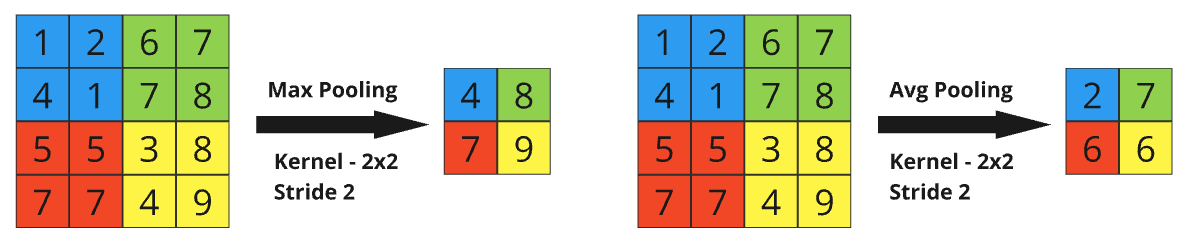
\includegraphics[width=0.8\linewidth]{img/pooling.png}
    \caption[Ejemplos de pooling utilizados en CNN.]{Ejemplos de pooling utilizados en CNN. A la izquierda, se muestra el max pooling, donde se selecciona el valor máximo de una determinada región (en este caso 2x2). A la derecha, se muestra el average pooling, donde se selecciona el valor promedio de la región influida por el filtro. Imagen original del autor.}\label{fig:pooling}
\end{figure}

\subsubsection{Capa totalmente conectada}

Las capas totalmente conectadas o densas (\emph{fully connected}) son un componente fundamental en las redes neuronales, presentes tanto en las tradicionales, formando la arquitectura básica de una ANN, como en las redes convolucionales. Estas capas se encuentran normalmente en las etapas finales de la red, encargándose de realizar la interpretación final de las características extraídas por las capas anteriores (véase~\autoref{fig:cnn}).\newline

Antes de entrar a una capa densa, la salida de las capas anteriores debe aplanarse (\emph{flattening}) en un vector unidimensional puesto que, generalmente, la salida de las capas anteriores tendrán forma matricial o tensorial, lo que impide que puedan ser procesadas directamente por las capas densas. De esta manera, el número de unidades de la primera capa densa se corresponde con el número de componentes del vector unidimensional.\newline

Estas capas combinan y procesan las características extraídas de las capas anteriores y tienen la posibilidad de capturar relaciones globales al conectar cada unidad de una capa con todas las unidades de la siguiente capa por medio de conexiones con pesos entrenables, lo que produce que la mayor parte de los pesos entrenables de una red suelan concentrarse en estas capas debido al elevado número de conexiones que presentan.\newline

\subsubsection{Capa de activación}\label{subsubsec:capa-de-activacion}

Las capas o funciones de activación son las responsables de introducir no linealidad en el modelo, transformando la combinación lineal de las entradas mediante una función matemática. Esta transformación es esencial para que la red pueda aprender y representar patrones complejos en los datos.\newline

Sin funciones de activación, una red neuronal se reduciría simplemente a una combinación lineal de las entradas, sin importar cuántas capas tuviera. Incluso si solo se usaran funciones de activación lineal, la red neuronal se comportaría como una función lineal. Como menciona Bishop en su libro: ``Si se considera que las funciones de activación de todas las unidades ocultas de una red son lineales, entonces para cualquier red de este tipo siempre podemos encontrar una red equivalente sin unidades ocultas'' (\cite{Bishop2006}), limitando la capacidad de la red para modelar relaciones complejas.\newline

Por tanto, las capas de activación se colocan después de cada capa lineal (como las capas convolucionales o las capas densas) en una red neuronal, con el objetivo de permitir que dicha capa pueda aprender también relaciones no lineales. A lo largo de este trabajo, se utilizarán algunas de las funciones de activación más comunes y ampliamente empleadas en el campo del aprendizaje profundo, entre las que se incluyen:

\begin{itemize}
    \item \textbf{ReLU (Rectified Linear Unit)}: Es una de las funciones de activación más utilizadas, especialmente en las capas ocultas de las redes neuronales profundas, debido a su simplicidad computacional, lo que permite acelerar el proceso de entrenamiento. Su expresión matemática es la siguiente
    
    \[
        \text{ReLU}(x) = \max(0, x)
    \]

    donde $x$ representa la entrada a la función, que corresponde con la salida lineal de la capa anterior de la red neuronal. Sin embargo, esta función de activación puede provocar el problema de ``neuronas muertas'', donde algunas unidades dejan de activarse permanentemente, cuando su entrada es negativa o $0$ (véase~\autoref{fig:funcionesactivacion}).

    \item \textbf{Softmax:} Se utiliza principalmente en la capa de salida para tareas de clasificación multiclase. Convierte un vector de valores reales en un vector de probabilidades que suman $1$, facilitando la interpretación de las salidas como probabilidades de pertenencia a cada clase. Su expresión matemática es la siguiente
 
    \[
        \text{Softmax}(x_i) = \frac{e^{x_i}}{\sum_{j=1}^{K} e^{x_j}}
    \]

    donde $x_i$ representa la entrada correspondiente a la clase $i$-ésima antes de aplicar la activación y $K$ el número de clases. Esta función de activación es una generalización de la función sigmoide para clasificación multiclase. Por tanto, para el caso de $K=2$ (clasificación binaria), esta función se reduce a la función sigmoide.\newline

\end{itemize}

\begin{figure}[h]
    \centering
    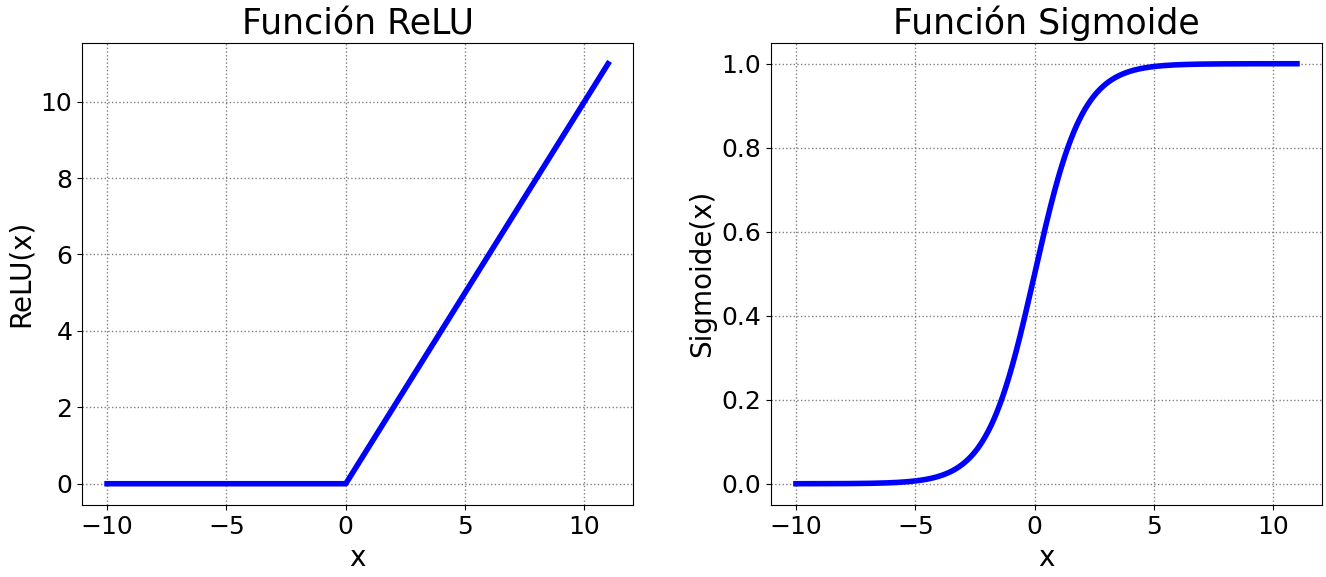
\includegraphics[width=0.8\linewidth]{img/funcionesactivacion.png}
    \caption[Ejemplos de funciones de activación utilizadas en CNN.]{Ejemplos de funciones de activación utilizadas en CNN. A la izquierda, se muestra la función ReLU, donde se observa como deja invariante los valores positivos, estableciendo a cero los valores negativos. A la derecha, se muestra la función sigmoide, que mapea los valores de entrada a un rango entre $0$ y $1$. Imagen original del autor.}\label{fig:funcionesactivacion}
\end{figure}

\chapter{El dilema clásico del aprendizaje}\label{ch:dilema-aprendizaje}

En este capítulo, como preámbulo antes de adentrarnos en el \textit{Deep Double Descent}, presentaremos algunos conceptos básicos de la sabiduría clásica del aprendizaje automático que nos harán entender de manera más precisa el suceso. Las fuentes principales utilizadas a lo largo de este capítulo son extractos de~\cite{Mostafa2012, Bishop2006}.\newline

\section{Concepto de aprendizaje}\label{sec:concepto-de-aprendizaje}
El aprendizaje, dentro del marco del aprendizaje automático, puede considerarse como un proceso en el que se busca encontrar una función $g$ que aproxime lo máximo posible a la función objetivo $f$, que describe las relaciones y patrones subyacentes entre las entradas y salidas de los datos. Dado que la función objetivo es siempre desconocida, pues, en otro caso, no habría que aprender nada al conocer directamente la función objetivo, serán los propios datos etiquetados los que nos ayuden, mediante el entrenamiento de modelos, a obtener una función aproximadora de dicha función objetivo.\newline

En nuestro caso, de cara a trabajar con el aprendizaje supervisado, consideraremos los siguientes componentes del mismo:
\begin{itemize}
    \item Espacio muestral $\mathcal{X}$: representa el conjunto de todas las posibles entradas $x$ que el modelo puede recibir, tomadas de manera independiente siguiendo alguna (sin restricción) distribución de probabilidad $P$ en $\mathcal{X}$.
    \item Conjunto $\mathcal{Y}$: compuesto por todas las posibles salidas (etiquetas) que el modelo debe predecir.
    \item Función objetivo $f: \mathcal{X} \rightarrow \mathcal{Y}$, que representa la función objetivo y desconocida que asigna cada entrada $x \in \mathcal{X}$ a una salida $y \in \mathcal{Y}$.
    \item Un conjunto de datos de entrenamiento $\mathcal{D}$, formado por pares $(x, y)$ con $x \in \mathcal{X}$ y $y \in \mathcal{Y}$, donde $f(x) = y$.
    \item Un conjunto de hipótesis $\mathcal{H}$, donde se encontrarán todas las funciones candidatas que el modelo puede aprender para aproximar la función objetivo. Es decir, $\mathcal{H} = \{h: X \rightarrow Y / X \subseteq \mathcal{X}, Y \subseteq \mathcal{Y}\}$. 
    \item Un algoritmo de aprendizaje $\mathcal{A}$, que es el encargado de elegir una función candidata $h \in \mathcal{H}$ que aproxime a la función objetivo $f$.\newline
\end{itemize}

De este modo, el modelo de aprendizaje automático, por medio del algoritmo de aprendizaje, será el encargado de seleccionar la función candidata $g \in \mathcal{H}$ que mejor aproxime a la función objetivo $f$ utilizando el conjunto de datos de entrenamiento disponible, con el propósito de que la función candidata $g$ siga replicando a la función objetivo $f$ ante nuevos datos no disponibles.\newline

\begin{figure}[h]
    \centering
    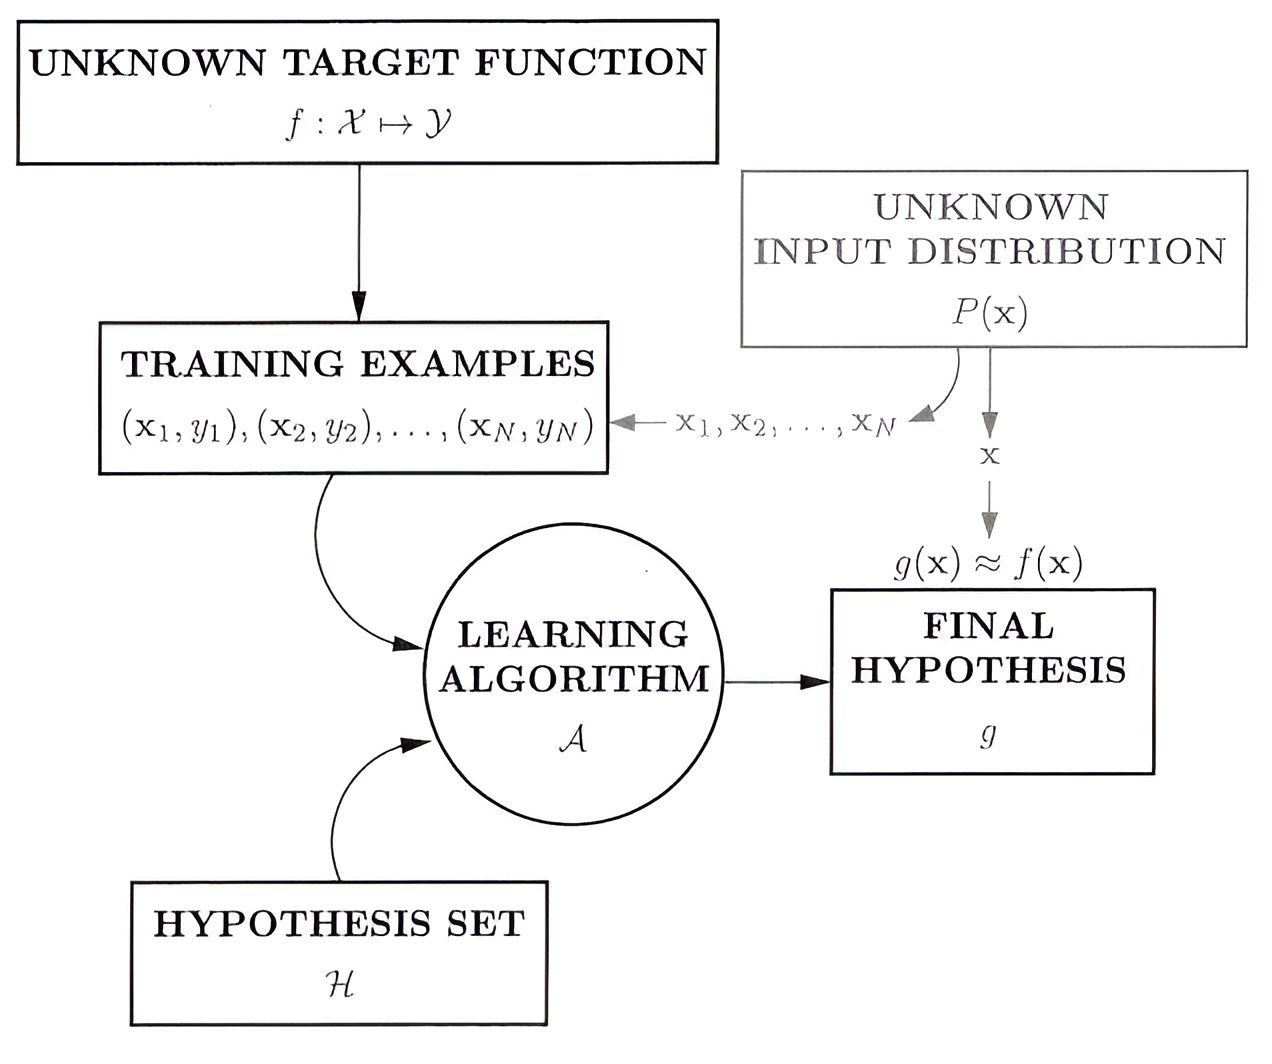
\includegraphics[width=0.7\linewidth]{img/learning-diagram.png}
    \caption[Diagrama representando el concepto básico de aprendizaje.]{Diagrama representando el concepto básico de aprendizaje~\cite{Mostafa2012}. El algoritmo de aprendizaje (\textit{learning algorithm}), utilizando los ejemplos de entrenamiento (\textit{training examples}) muestreados de una distribución de probabilidad desconocida (\textit{unknown input distribution}), buscará en el conjunto de hipótesis (\textit{hypothesis set}) la mejor aproximación (\textit{final hypothesis}) a la función objetivo desconocida (\textit{unknown target function}) que se desea aprender.}\label{fig:learning-diagram}
\end{figure}

\subsection{Descenso de gradiente y aprendizaje}\label{subsec:descenso-gradiente}

El descenso de gradiente o \emph{gradient descent} (GD) es la columna vertebral del aprendizaje en redes neuronales y, en general, sienta las bases para las técnicas de aprendizaje automático y aprendizaje profundo. Se trata de un algoritmo de optimización sin restricciones cuyo objetivo principal es minimizar la función de pérdida o error del modelo. Dicha función de pérdida mide cuán lejos están las predicciones realizadas por el modelo de los valores reales, y minimizarla conllevará asociada una mejora en la precisión y capacidad de generalización del modelo.\newline

La idea subyacente del descenso de gradiente se basa en calcular de forma iterativa el gradiente, es decir, la derivada parcial de la función de pérdida con respecto a los parámetros. A partir de este gradiente, nos desplazamos en la dirección opuesta al mismo (véase Ecuación~\eqref{eq:descenso-gradiente}), ya que esta zona indica la dirección del descenso más pronunciado en la función de pérdida. De este modo, se garantiza que los parámetros se ajusten para minimizar progresivamente la pérdida, mejorando así el rendimiento del modelo.\newline

A continuación se muestra la expresión del descenso de gradiente:

\begin{equation}
    \mathbf{w}^{(\tau + 1)} = \mathbf{w}^{(\tau)} - \eta \nabla E(\mathbf{w}^{(\tau)})
    \label{eq:descenso-gradiente}
\end{equation}

donde $\mathbf{w}^{(\tau + 1)}$ representa los valores de los parámetros actualizados, $\mathbf{w}^{(\tau)}$ representa los valores de los parámetros antes de la actualización, $\eta$ es un hiperparámetro, denominado tasa de aprendizaje o \emph{learning rate}, que controla el tamaño del paso en cada actualización y $\nabla E(\mathbf{w}^{(\tau)})$ indica el gradiente de la función de pérdida con respecto a los parámetros, es decir, la dirección y magnitud en la que la función de pérdida aumenta de manera más rápida.\newline

Es importante destacar que la tasa de aprendizaje ($\eta$) desempeña un papel esencial en el proceso de optimización. Si se elige un valor demasiado pequeño de la misma, el modelo podría tardar mucho en converger (véase~\autoref{fig:gradientdescent}), requiriendo un número elevado de épocas o iteraciones para alcanzar un mínimo adecuado de la función de pérdida. Por el contrario, si se selecciona un valor demasiado grande, el modelo podría no converger e incluso divergir, oscilando alrededor del mínimo sin lograr estabilizarse o incluso aumentando la pérdida. Es por esto que, la mejor estrategia suele consistir en utilizar un valor grande al inicio del entrenamiento, para acelerar el entrenamiento, y reducirlo progresivamente a medida que avanza, con el objetivo de no divergir y estabilizarnos en el mínimo.\newline

\begin{figure}[h]
    \centering
    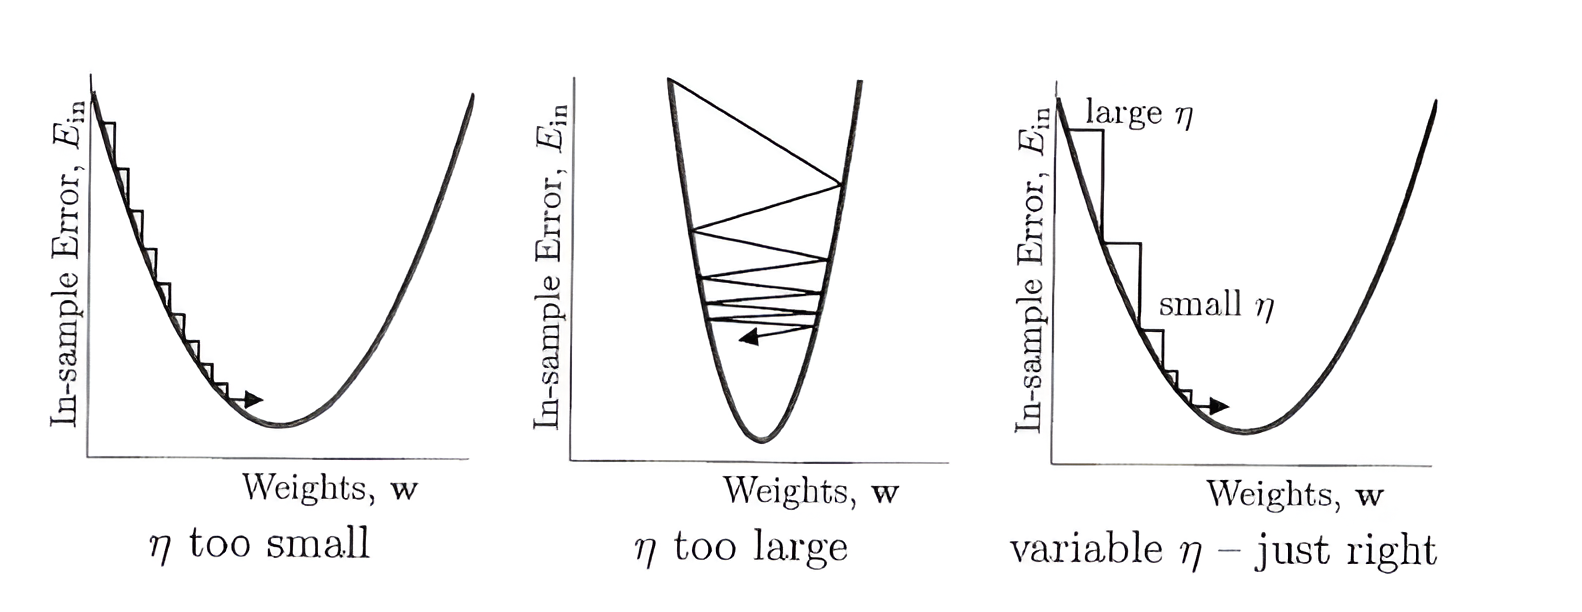
\includegraphics[width=0.9\linewidth]{img/gradientdescent.png}
    \caption[Distintas tasas de aprendizaje para el descenso de gradiente~\cite{Mostafa2012}.]{Distintas tasas de aprendizaje para el descenso de gradiente~\cite{Mostafa2012}. En la primera imagen, una tasa de aprendizaje pequeña lleva a una convergencia lenta con muchas actualizaciones. En la imagen central, una tasa demasiado grande provoca saltos bruscos que pueden impedir la convergencia. En la última imagen, una tasa variable comienza con un valor grande para avanzar rápido y disminuye progresivamente, logrando una convergencia rápida y estable.}\label{fig:gradientdescent}
\end{figure}

Asimismo, existen variantes del descenso de gradiente, como el descenso de gradiente estocástico (SGD), que actualiza los parámetros utilizando cada ejemplo de entrenamiento, lo que provoca que sea muy lento cuando trabajamos con grandes volúmenes de datos. Por otro lado, nos encontramos el descenso de gradiente por lotes (Batch Gradient Descent), que utiliza el conjunto completo de datos de entrenamiento para calcular el gradiente y actualizar los parámetros, lo que permite realizar una convergencia más estable y precisa. Sin embargo, suele ser más costoso tanto computacionalmente como en términos de tiempo. Es por esto que, en el desarrollo de este proyecto, se utilizará el descenso de gradiente por mini-lotes (Mini-batch Gradient Descent), que combina lo mejor de ambos métodos, ya que utiliza subconjuntos de datos de entrenamiento para realizar la actualización de parámetros.\newline

En resumen, el descenso de gradiente permite que la red neuronal mejore sus predicciones a lo largo de múltiples iteraciones o épocas. Cada vez que el modelo procesa un conjunto de datos, calcula el error y ajusta sus parámetros para aprender de los errores cometidos, repitiéndose este proceso hasta que la función de pérdida alcanza un valor mínimo aceptable.\newline

\subsubsection{Optimizador Adam}\label{subsubsec:optimizador-adam}
De cara al interés de nuestro proyecto, trabajaremos con el optimizador \textbf{Adam} (\textit{Adaptive Moment Estimation},~\cite{Diederik2017}). Este optimizador se basa en las ideas de los algoritmos \textbf{Momentum} y \textbf{RMSProp}, combinando sus principales ventajas para lograr una convergencia más rápida y estable durante el entrenamiento de modelos de aprendizaje profundo.\newline

El método de \textit{Momentum} mejora al SGD acumulando un promedio móvil de los gradientes pasados. La actualización de los parámetros se realiza de la siguiente forma:

\[
    \begin{aligned}
        m_{\tau} &= \beta_1 \cdot m_{\tau-1} + (1 - \beta) \cdot \nabla E(w_{\tau - 1}), \\
        w_{\tau} &= w_{\tau - 1} - \eta \cdot m_\tau
    \end{aligned}
\]

donde el término $\beta$ actúa como un factor de decaimiento que regula la influencia de los gradientes anteriores en la actualización actual. Por su parte, $\eta$ representa la tasa de aprendizaje. Así, la variable $m_{\tau}$ corresponde al promedio móvil de los gradientes, es decir, una estimación de primer orden que suaviza la dirección de la actualización.\newline

El algoritmo \textit{RMSProp} adapta la tasa de aprendizaje en función de la magnitud reciente de los gradientes. Para lograrlo, calcula un promedio móvil de los cuadrados de los gradientes, lo que permite ajustar dinámicamente la escala de la actualización para cada parámetro:

\[
    \begin{aligned}
        v_{\tau} &= \beta \cdot v_{\tau-1} + (1- \beta)(\nabla E(w_{\tau-1})), \\
        w_{\tau} &= w_{\tau-1} - \eta \cdot \frac{\nabla E(w_{\tau-1})}{\sqrt{v_{\tau}}+\epsilon},
    \end{aligned}
\]

donde el factor $\beta$ actúa, al igual que en el caso de Momentum, como un factor de olvido que determina cuánto influyen los valores anteriores en la media móvil. Así, $v_{\tau}$ representa una estimación de segundo orden, correspondiente al promedio móvil de los cuadrados de los gradientes. Además, el término $\epsilon$ se introduce para mejorar la estabilidad numérica, evitando divisiones por cero durante la actualización de los parámetros.\newline

Finalmente, \textit{Adam} combina los enfoques anteriores, manteniendo simultáneamente estimaciones de primer y segundo orden. Las actualizaciones se realizan de la siguiente manera:

\begin{equation}
    \begin{aligned}
        m_{\tau} &= \beta_1 \cdot m_{\tau-1} + (1 - \beta_1) \cdot \nabla E(w_{\tau - 1}), \\
        v_{\tau} &= \beta_2 \cdot v_{\tau-1} + (1 - \beta_2) \cdot \nabla E(w_{\tau - 1}).
    \end{aligned}
\end{equation}

Dado que $m_\tau$ y $v_\tau$ están inicializados en cero, Adam introduce una corrección de sesgo:

\begin{equation}
    \begin{aligned}
        \hat{m_\tau} = \frac{m_\tau}{1- \beta_1^{\tau}}, \\
        \hat{v_\tau} = \frac{v_\tau}{1- \beta_2^{\tau}}.
    \end{aligned}
\end{equation}

Como paso final, los parámetros se actualizan de la siguiente forma:

\begin{equation}
    w_{\tau} = w_{\tau - 1} - \frac{\eta}{\sqrt{\hat{v}_{\tau}} + \epsilon} \cdot \hat{m}_{\tau}.
\end{equation}

Este enfoque combina la dirección promedio de los gradientes con una tasa de aprendizaje adaptativa. Por un lado, acumular gradientes pasados permite suavizar la trayectoria y evitar oscilaciones y por otro, normalizar mediante una estimación de segundo orden ajusta la tasa de aprendizaje de manera dinámica para cada parámetro. Así, Adam consigue una optimización más eficiente, estable y con mejor convergencia en escenarios complejos o de alta dimensión.\newline

\subsubsection{Aprendizaje en una red neuronal}\label{subsubsec:aprendizaje-red-neuronal}

Como se comentó en la \autoref{sec:redes-neuronales-artificiales}, la primera fase del aprendizaje consiste en la transmisión de la información desde la capa de entrada hacia la capa de salida, pasando por las capas ocultas, proceso conocido como propagación hacia delante o \emph{forward pass}. Durante este proceso, las entradas se multiplican por los pesos de la red, se suman los sesgos o \emph{biases}, consistente en un parámetro adicional que se suma al resultado de la combinación lineal antes de pasar por la función de activación, cuya función principal es permitir que el modelo ajuste su salida de manera más flexible, sin estar forzado a pasar por el origen de coordenadas y, finalmente, se aplican las funciones de activación para introducir no linealidad. Este flujo de datos permite que el modelo genere una predicción para cada entrada.\newline

\begin{figure}[h]
    \centering
    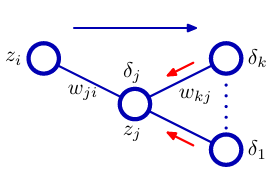
\includegraphics[width=0.3\linewidth]{img/aprendizajegd.png}
    \caption[Proceso de retropropagación del error~\cite{Bishop2006}.]{Proceso de retropropagación del error~\cite{Bishop2006}. Dado un lote de entrenamiento, se propaga la información hacia delante (flecha azul), se calculan las activaciones y el error de salida. Seguidamente, se realiza el paso hacia atrás (flechas rojas), calculando el error $\delta_j$ de cada unidad $j$ en cada capa. Finalmente, se actualizan los parámetros utilizando el gradiente calculado.}\label{fig:aprendizajegd}
\end{figure}

Una vez obtenida la predicción, se calcula la función de pérdida para evaluar la discrepancia entre la predicción y el valor real. De esta manera, podemos describir la salida resultante de cualquier neurona mediante la siguiente expresión, extraída de~\cite{Prince2023}:

\begin{equation}
    h_d = \phi \left( w_{d0} + \sum_{i=1}^{D_i} w_{di} x_i \right)
    \label{eq:hidden_unit}
\end{equation}

donde $d$ hace referencia a la neurona en dicha posición, $\phi$ representa una función de activación no lineal, $x_i \in \mathbb{R}^{D_i}$ representa la entrada multidimensional, donde $D_i$ es el número de características de entrada (en este caso consideramos nuestro conjunto de datos de entrenamiento $\mathcal{D}$ como un subconjunto de $\mathbb{R}^{D_i}$) y $w_{di}$ con $i \in \{0,1,\ldots,D_i\}$ representa los pesos que conectan la entrada $x_i$ con la neurona $d$, donde para $i = 0$ se obtiene el término del sesgo.\newline

Seguidamente, se inicia la segunda fase del aprendizaje, cuyo objetivo es ajustar los parámetros de la red para minimizar ese error. Para ello, se utiliza retropropagación del error o \emph{backpropagation}, que calcula el gradiente de la función de pérdida con respecto a los pesos y sesgos, mediante la regla de la cadena del cálculo diferencial. Posteriormente, el algoritmo de descenso de gradiente actualiza los pesos en la dirección opuesta al gradiente.\newline

En conlusión, el forward pass y la backpropagation trabajan de manera conjunta para permitir que la red neuronal aprenda de manera efectiva. El forward pass genera las predicciones para los datos de entrada, la función de pérdida evalúa el error cometido en dichas predicciones, la backpropagation calcula la contribución de cada unidad a dicho error (véase~\autoref{fig:aprendizajegd}) y, por último, el descenso de gradiente ajusta los parámetros para mejorar las predicciones futuras, repitiéndose este ciclo a lo largo de múltiples iteraciones.\newline

\section{Bias-variance tradeoff}\label{sec:capitulo-bias-variance-tradeoff}
El objetivo del aprendizaje radica en obtener un bajo error de prueba o generalización ($E_{out}$) sobre datos desconocidos, lo que implicará que hemos conseguido aproximar de buena manera la función objetivo $f$. La capacidad para conseguir un bajo error de generalización está ligada directamente al conjunto de hipótesis ($\mathcal{H}$), donde si nuestro conjunto es suficientemente grande tendremos una mayor probabilidad de aproximar la función objetivo $f$, al disponer de un mayor número de funciones candidatas. Sin embargo, si nuestro conjunto $\mathcal{H}$ es demasiado grande, puede darse el caso de que, al elegir una de las funciones candidatas (usando nuestro conjunto de entrenamiento), dicha función no sea la que mejor aproxime a la función objetivo, lo que provoque un mayor error de generalización. A este problema se le conoce como el problema del \textit{equilibrio entre aproximación y generalización}. Adicionalmente, el conjunto de hipótesis ideal sería el formado únicamente por la función objetivo, es decir, $\mathcal{H} = \{f\}$.\newline

El análisis sesgo-varianza o \emph{bias-variance analysis} busca descomponer el error de generalización en dos términos principales:

\begin{enumerate}
    \item Cómo de bien puede $\mathcal{H}$ aproximar a la función objetivo $f$ en general, no solo en la muestra.
    \item Hasta qué punto podemos acercanos a una buena función candidata $g \in \mathcal{H}$.\newline
\end{enumerate}

Adicionalmente, el error de generalización $E_{out}$ incluye un término adicional conocido como \textit{ruido}. Este término hace referencia al error irreducible que se encuentra de manera natural en los datos y que, generalmente, es debido a factores fuera del control del modelo, tales como mediciones imprecisas o variables no modeladas. Dado que este tipo de error es inevitable y no puede ser reducido, no se considera relevante en la descomposición del error. Sin embargo, cabe destacar que este ruido suele ser una limitación fundamental de la generalización del modelo.\newline

\subsection{Formulación matemática del $E_{out}$}\label{sec:formulacion-matematica-Eout}
A continuación, detallaremos matemáticamente las componentes del error fuera de la muestra o de generalización. Para ello y con objeto de simplificar la descomposición del $E_{out}$ de manera limpia en los dos términos principales citados anteriormente, vamos a considerar un problema de regresión que no presenta ruido en los datos, utilizando el error cuadrático como medida de evaluación del error.\newline

Sea $g^{\mathcal{(D)}} \in \mathcal{H}$ nuestra función candidata elegida (hipótesis final), que dependerá del conjunto de datos utilizado ($\mathcal{D}$). Destacamos que, dado cualquier otro conjunto de datos, encontraremos una hipótesis final distinta.\newline

El \emph{error de generalización o error fuera de la muestra}, definido como la diferencia entre la predicción del modelo y los valores reales en un conjunto de datos no visto durante el entrenamiento, quedaría expresado de la siguiente forma:
\begin{equation}\label{eq:E_out1}
    E_{out}(g^{\mathcal{(D)}}) = \mathbb{E}_{x}[{(g^{\mathcal{(D)}}(x) - f(x))}^2], \quad x \notin \mathcal{D}
\end{equation}

donde $\mathbb{E}_{x}$ denota el valor esperado con respecto a $x$ (basado en la distribución de probabilidad del espacio de entrada $\mathcal{X})$, con el objetivo de obtener el valor esperado del error en todo el espacio.\newline

Dado que la ecuación~\eqref{eq:E_out1} depende de un conjunto de datos en particular, podemos eliminar esta dependencia del conjunto de datos utilizado tomando el valor esperado de dicho error con respecto a todos los conjuntos de datos:

\begin{equation}\label{eq:E_out2}
    \mathbb{E}_{\mathcal{D}}[E_{out}(g^{\mathcal{(D)}})] = \mathbb{E}_{\mathcal{D}}[\mathbb{E}_{x}[{(g^{\mathcal{(D)}}(x) - f(x))}^2]]. 
\end{equation}\newline

Cambiamos ahora el orden de las esperanzas dado que, en realidad, estamos integrando y cambiando el orden de integración, que podemos realizarlo dado que el integrando ${(g^{\mathcal{(D)}}(x) - f(x))}^2$ es estrictamente no negativo:

\begin{equation}\label{eq:E_out3}
    \mathbb{E}_{\mathcal{D}}[E_{out}(g^{\mathcal{(D)}})] = \mathbb{E}_{x}[\mathbb{E}_{\mathcal{D}}[{(g^{\mathcal{(D)}}(x) - f(x))}^2]].
\end{equation}\newline

Nos centramos en calcular $\mathbb{E}_{\mathcal{D}}[{(g^{\mathcal{(D)}}(x) - f(x))}^2]$, olvidándonos por ahora del valor esperado sobre $x$, dado que nos interesa calcular la esperanza con respecto a $\mathcal{(D)}$ hasta obtener una descomposición limpia del error. Para ello, vamos a definir el concepto de hipótesis promedio $\bar{g}(x)$ de la siguiente manera:

\begin{equation}\label{eq:gbar}
    \bar{g}(x) = \mathbb{E}_{\mathcal{D}}[g^{\mathcal{(D)}}(x)]
\end{equation}

que corresponde al valor esperado de todas las hipótesis que podemos obtener al aprender de los distintos conjuntos de datos que utilicemos. Destacamos que, en la ecuación~\eqref{eq:gbar}, tenemos $x$ (punto de prueba) fijo, por lo que $g^{\mathcal{(D)}}(x)$ es una variable aleatoria determinada por la elección de nuestros datos, donde si tomamos distintos conjuntos de datos, obtendremos distintos valores para la hipótesis en el punto $x$ fijado. Sin embargo, en la realidad nunca dispondremos de esta hipótesis promedio, pues tendríamos un número infinito de conjuntos de datos distintos. Además, cabe destacar que la hipótesis promedio no tiene asegurada su pertenencia al conjunto de hipótesis $\mathcal{(H)}$, aunque sea el promedio de hipótesis pertenecientes a $\mathcal{H}$.\newline

Continuando con la descomposición, tenemos el siguiente resultado:

\begin{equation}\label{eq:E_out4}
    \mathbb{E}_{\mathcal{D}}[{(g^{\mathcal{(D)}}(x) - f(x))}^2] = \mathbb{E}_{\mathcal{D}}[{(g^{\mathcal{(D)}}(x) - \bar{g}(x) + \bar{g}(x) - f(x))}^2]
\end{equation}

donde se ha sumado y restado la misma cantidad ($\bar{g}(x)$) para simplificar la descomposición.\newline

Seguidamente, continuamos desarrollando el término cuadrático de la ecuación~\eqref{eq:E_out4}:

\[ \mathbb{E}_{\mathcal{D}}[{(g^{\mathcal{(D)}}(x) - \bar{g}(x))}^2 + {(\bar{g}(x) - f(x))}^2 + 2(g^{\mathcal{(D)}}(x) - \bar{g}(x))(\bar{g}(x) - f(x))]. \]\newline

Dado que estamos realizando el valor esperado con respecto a $\mathcal{D}$, de la ecuación anterior tenemos que $(\bar{g}(x) - f(x))$ es una constante. Por tanto, dado que el valor esperado de una constante es la propia constante, para obtener el valor esperado del término cruzado solo necesitamos conocer el valor esperado de $(g^{\mathcal{(D)}}(x) - \bar{g}(x))$:

\begin{equation}\label{eq:E_out6}
    \mathbb{E}_{\mathcal{D}}[g^{\mathcal{(D)}}(x) - \bar{g}(x)] = \mathbb{E}_{\mathcal{D}}[g^{\mathcal{(D)}}(x)] - \mathbb{E}_{\mathcal{D}}[\bar{g}(x)] = \bar{g}(x) - \bar{g}(x) = 0.
\end{equation}\newline

Finalmente, de la ecuación~\eqref{eq:E_out4} nos queda la siguiente expresión:

\begin{equation}\label{eq:E_out7}
    \mathbb{E}_{\mathcal{D}}[{(g^{\mathcal{(D)}}(x) - f(x))}^2] = \mathbb{E}_{\mathcal{D}}[{(g^{\mathcal{(D)}}(x) - \bar{g}(x))}^2] + {(\bar{g}(x) - f(x))}^2
\end{equation}

donde hemos usado que el valor esperado de una constante $(\bar{g}(x) - f(x))$ es igual a dicha constante.\newline

Por consiguiente, hemos obtenido una descomposición de la ecuación~\eqref{eq:E_out4} en dos términos que serán los asociados a los términos de varianza (\textit{variance}) y sesgo (\textit{bias}) respectivamente.

\begin{enumerate}
    \item $\mathbb{E}_{\mathcal{D}}[{(g^{\mathcal{(D)}}(x) - \bar{g}(x))}^2]$: nos indica cómo de lejos se encuentra nuestra hipótesis, $g^{\mathcal{(D)}}(x)$, obtenida de un conjunto de datos particular de la mejor (promedio) hipótesis, $\bar{g}(x)$, que podemos obtener utilizando nuestro conjunto de hipóstesis $\mathcal{H}$. Este es el término asociado a la varianza de $x$ ($\textbf{var(x)}$).
    \item ${(\bar{g}(x) - f(x))}^2$: nos indica cómo de lejos se encuentra dicha hipótesis ideal, $\bar{g}(x)$, de la función objetivo $f(x)$. Este es el término asociado al sesgo de $x$ ($\textbf{bias(x)}$).\newline
\end{enumerate}

Por tanto, volviendo a la ecuación~\eqref{eq:E_out3} nos queda:

\begin{equation}\label{eq:E_out8}
    \mathbb{E}_{\mathcal{D}}[E_{out}(g^{\mathcal{(D)}})] = \mathbb{E}_{x}[\mathbb{E}_{\mathcal{D}}[{(g^{\mathcal{(D)}}(x) - f(x))}^2]] = \mathbb{E}_{x}[\textbf{var(x)} + \textbf{bias(x)}]
\end{equation}

donde denotaremos por \textbf{sesgo} a $\mathbb{E}_{x}[\textbf{bias(x)}]$ y por \textbf{varianza} a $\mathbb{E}_{x}[\textbf{var(x)}]$.\newline

\begin{observacion}
    Cuando hay ruido presente en los datos de entrenamiento, es decir, $y(x) = f(x) + \epsilon(x)$ y, además, $\epsilon$ es una variable aleatoria con media $0$ y varianza $\sigma^{2}$, entonces

    \[ E_{out}(g^{(\mathcal{D})}) = \mathbb{E}_{x, y}[g^{(\mathcal{D})}(x)-{y(x)}^{2}] \]

    y, en este caso, se verifica

    \[ \mathbb{E}_{\mathcal{D}}[E_{out}(g^{(\mathcal{D})})] = \sigma^{2} + bias + var. \]
\end{observacion}

\begin{proof}
    Dado que asumimos que $\epsilon$ es una variable aleatoria con media $0$, obtenemos que $\mathbb{E}[\epsilon(x)] = 0$.

    \begin{equation}\label{eq:E_out-noise1}
        \mathbb{E}_{\mathcal{D}, \epsilon}[{(g^{\mathcal{(D)}}(x) - y(x))}^2] = \mathbb{E}_{\mathcal{D}, \epsilon}[{(g^{\mathcal{(D)}}(x) - f(x)) - \epsilon(x)}^2]
    \end{equation}

    donde dado que $y$ depende del ruido, consideramos también el valor esperado con respecto a $\epsilon$ que afectará únicamente a $y$. Procediendo de manera similiar a la Ecuación~\eqref{eq:E_out4}, obtenemos

    \begin{equation}
        \mathbb{E}_{\mathcal{D}, \epsilon}[{(g^{\mathcal{(D)}}(x) - \bar{g}(x) + \bar{g}(x) - f(x) - \epsilon(x))}^2]
    \end{equation}

    y, tras realizar operaciones, llegamos a

    \begin{equation}
        \mathbb{E}_{\mathcal{D}, \epsilon}[{(g^{\mathcal{(D)}}(x) - f(x))}^2] + 2\mathbb{E}_{\mathcal{D}, \epsilon}[(g^{\mathcal{(D)}}(x)-f(x))\epsilon(x)] + \mathbb{E}_{\mathcal{D}, \epsilon}[\epsilon^{2}(x)]
    \end{equation}

    donde el primer sumando no depende de $\epsilon$, el tercer sumando no depende de $\mathcal{D}$ y el segundo sumando puede expresarse de la siguiente forma:

    \begin{equation}
        2\mathbb{E}_{\mathcal{D}, \epsilon}[(g^{\mathcal{(D)}}(x)-f(x))\epsilon(x)] = 2\mathbb{E}_{\mathcal{D}, \epsilon}[(g^{\mathcal{(D)}}(x)-f(x))]\mathbb{E}_{\mathcal{D}, \epsilon}[\epsilon(x)].
    \end{equation}

    donde el valor esperado con respecto a $\epsilon$ no depende de $\mathcal{D}$. De esta manera y conociendo que $\mathbb{E}_{\epsilon}[\epsilon(x)] = 0$ y $\mathbb{E}_{\epsilon}[{\epsilon(x)}^{2}] = \sigma^{2}$, obtenemos que la Ecuación~\eqref{eq:E_out-noise1} puede expresarse de la siguiente forma

    \begin{equation}
        \mathbb{E}_{\mathcal{D}, \epsilon}[{(g^{\mathcal{(D)}}(x) - y(x))}^2] = \mathbb{E}_{\mathcal{D}}[{(g^{\mathcal{(D)}}(x) - f(x))}^2] + \sigma^{2}.
    \end{equation}

    Finalmente, aplicando el valor esperado sobre $x$ a la expresión anterior, obtenemos el resultado buscado.\newline
\end{proof}

Como conclusión de esta sección, detallaremos algunos aspectos clave del análisis del sesgo y de la varianza:

\begin{itemize}
    \item Aunque el análisis de sesgo-varianza se basa en la medida del error cuadrático, el algoritmo de aprendizaje utilizado por el modelo no tiene que basarse en minimizar el error cuadrático. Es decir, se puede usar cualquier otro criterio (función de pérdida) para producir $g^{\mathcal{(D)}}$ basado en el conjunto de datos $\mathcal{D}$ y, una vez que tenemos $g^{\mathcal{(D)}}$, calculamos su sesgo y varianza utilizando el error cuadrático.
    \item El sesgo y la varianza no pueden ser calculados en la práctica, ya que dependen de la función objetivo y de la distribución de probabilidad de la entrada (ambas desconocidas), por lo que su descomposición resulta de utilidad como una herramienta conceptual a la hora de entender y desarrollar un modelo.\newline
    
\end{itemize}

\section{Equilibrio clásico entre sesgo y varianza}\label{sec:equilibrio-sesgo-varianza}
Siguiendo con los resultados obtenidos en la \autoref{sec:formulacion-matematica-Eout}, nuestro objetivo ahora es minimizar el error fuera de la muestra, inducido por tres componentes: ruido, sesgo y varianza. Dado que, como se ha comentado previamente, el rudio es irreducible y no hay nada que podamos hacer para evitarlo, nos centraremos en intentar reducir los dos términos principales reducibles del error: el sesgo y la varianza.\newline

Conocemos que el sesgo viene definido por la medida en la que la predicción ideal obtenida de todos los conjuntos de datos difiere de la función objetivo, o expresado de manera similar, el sesgo es el resultado de la incapacidad del modelo para describir la función objetivo. Este resultado sugiere que podemos reducir este término de error haciendo que nuestro modelo sea más flexible, es decir, aumentando nuestro conjunto de hipótesis $\mathcal{H}$ (haciéndolo más complejo), con el objetivo de disponer de un mayor número de funciones candidatas para forzar que la hipótesis promedio se aproxime lo máximo posible a la función objetivo.\newline

Por otro lado, la varianza viene a ofrecernos la medida en la que varían las hipótesis para distintos conjuntos de datos con respecto a la hipótesis ideal, o expresado de manera similar, la varianza evalúa cómo de sensible es una hipótesis a la selección específica del conjunto de datos $\mathcal{D}$. Este análisis revela que podemos reducir este término de error disminuyendo el conjunto de hipótesis ya que, en un espacio de hipótesis restringido, al haber menos hipótesis, las hipótesis son menos sensibles a las variaciones en el conjunto de datos. Como resultado, al cambiar el conjunto de datos para seleccionar una hipótesis, es más probable que se elijan hipótesis similares.\newline

En consecuencia, observamos una dependencia de ambos términos de error con respecto a la complejidad del conjunto de hipótesis ($\mathcal{H}$) utilizado. Esta dependencia viene dada por:

\begin{itemize}
    \item Al aumentar la complejidad del conjunto de hipótesis, es decir, al incrementar su tamaño, el sesgo disminuirá, pero la varianza irá aumentado.
    \item Si reducimos la complejidad del conjunto de hipótesis, es decir, disminuimos su tamaño, el sesgo irá aumentando, pero la varianza disminuirá.\newline
\end{itemize}

De este modo, el equilibrio buscado en esta sección con objeto de minimizar el error fuera de la muestra viene ligado a la elección de un conjunto de hipótesis ($\mathcal{H}$) suficientemente complejo como para acercanos a la función objetivo y suficientemente simple como para no disponer de una cantidad excesiva de hipótesis que induzcan un alto grado de varianza. Este equilibrio se podrá conseguir mediante diversas técnicas, como la regularización, que se explicarán en secciones posteriores.\newline

\begin{figure}[h]
    \centering
    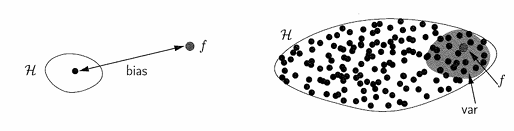
\includegraphics[width=0.7\linewidth]{img/bias-variance.png}
    \caption[Distintos casos del conjunto de hipótesis y de la función objetivo.] {Distintos casos del conjunto de hipótesis y de la función objetivo~\cite{Mostafa2012}. A la izquierda observamos como nuestro conjunto de hipótesis presenta únicamente una función candidata, alejada de la función objetivo $f$, lo que implica un alto sesgo y una varianza nula. A la derecha observamos un conjunto de hipótesis con numerosas funciones candidatas que incluye a la función objetivo $f$, por lo que el sesgo es muy cercano a $0$ y la varianza es grande.}\label{fig:bias-variance}
\end{figure}

\subsection{Curva de aprendizaje}

Para finalizar este capítulo, introduciremos el concepto de curva de aprendizaje o \emph{learning curve}, que será la principal herramienta que utilizaremos a lo largo de todo el proyecto para analizar el rendimiento de los distintos modelos que utilicemos.\newline

En primer lugar y de manera análoga a la ecuación~\eqref{eq:E_out1}, definimos el \emph{error de entrenamiento o error dentro de la muestra ($E_{in}$)} como la diferencia entre la predicción del modelo y los valores reales del conjunto de datos de entrenamiento, es decir

\begin{equation}\label{eq:E_in1}
    E_{in}(g^{\mathcal{(D)}}) = \mathbb{E}_{x}[{(g^{\mathcal{(D)}}(x) - f(x))}^2], \quad x \in \mathcal{D}.
\end{equation}\newline

Por consiguiente, después de aprender de un conjunto particular de datos $\mathcal{D}$ de tamaño $N$, la hipótesis final elegida $g^{(\mathcal{D})}$ tendrá error de entrenamiento ($E_{in}(g^{(\mathcal{D})})$) y error de generalización ($E_{out}(g^{(\mathcal{D})})$), ambos dependiendo del conjunto de datos utilizado. Como se comentó en la \autoref{sec:formulacion-matematica-Eout}, al realizar la esperanza con respecto a todos los conjuntos de datos de dichos errores obtenemos los errores esperados $\mathbb{E}_{\mathcal{D}}[E_{in}(g^{(\mathcal{D})})]$ y $\mathbb{E}_{\mathcal{D}}[E_{out}(g^{(\mathcal{D})})]$, donde ambos errores son funciones del tamaño del conjunto de datos ($N$).\newline

\begin{figure}[h]
    \centering
    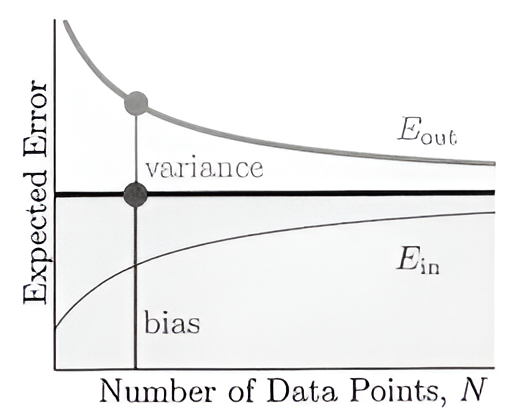
\includegraphics[width=0.4\linewidth]{img/learning-curve.png}
    \caption[Ejemplo de curva de aprendizaje tradicional~\cite{Mostafa2012}.] {Ejemplo de curva de aprendizaje tradicional~\cite{Mostafa2012}. Observamos la curva de aprendizaje de un modelo con respecto al tamaño del conjunto de datos. Se puede comprobar como el $E_{out}$ decrece, mientras que el $E_{in}$ crece. Además, se puede apreciar la descomposición sesgo-varianza, donde la línea central en negrita denota la hipótesis promedio.}\label{fig:learning-curve-bias-variance}
\end{figure}

Denominaremos \emph{curva de aprendizaje} a la representación gráfica que muestra la relación entre el rendimiento de un modelo y el tamaño del conjunto de datos utilizado para su entrenamiento, es decir, a la gráfica que incluye los errores esperados $\mathbb{E}_{\mathcal{D}}[E_{in}(g^{(\mathcal{D})})]$ y $\mathbb{E}_{\mathcal{D}}[E_{out}(g^{(\mathcal{D})})]$ como función de $N$.\newline

Además, dado que la curva de aprendizaje está ligada a los errores esperados del modelo tanto dentro como fuera de la muestra, podríamos analizar el equilibrio sesgo-varianza directamente sobre dicha gráfica. Sin embargo, para llevar a cabo dicho análisis, necesitaríamos conocer la hipótesis promedio $\bar{g}$ que, como sabemos de secciones anteriores, es imposible de calcular. No obstante, si tuvieramos dicha hipótesis promedio, podríamos realizar el análisis (véase \autoref{fig:learning-curve-bias-variance}), teniendo en cuenta que el $E_{out}$ es suma de sesgo y varianza (obviando el término de ruido).\newline

Sin embargo, de cara a analizar el doble descenso a lo largo del proyecto, \textbf{no utilizaremos directamente la curva de aprendizaje} tal y como se ha definido, dado que nuestro objetivo es analizar el error con respecto a la capacidad del modelo y no en función del número de datos utilizados. Es por esto que, nuestra curva de aprendizaje será una modificación de la curva de aprendizaje original, donde en el eje $X$ de la gráfica aparecerá indistintamente la capacidad o el número de épocas de entrenamiento del modelo y en el eje $Y$ el error esperado (véase~\autoref{fig:learning-curve-classicalvsmodern}), tanto dentro como fuera de la muestra, para un número fijo de datos de entrenamiento.\newline

\begin{figure}[h]
    \centering
    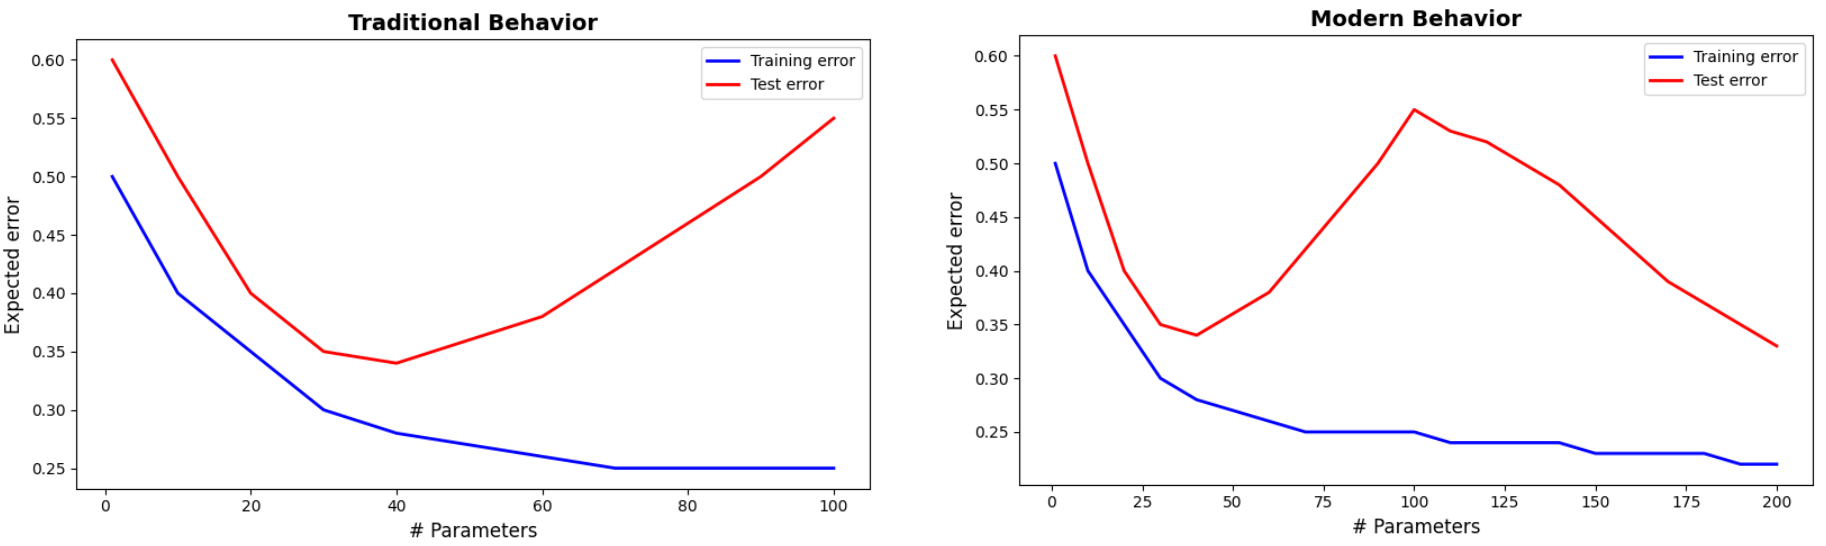
\includegraphics[width=0.9\linewidth]{img/learning-curve-classicalvsmodern.png}
    \caption[Ejemplos de curvas de aprendizaje modificadas para este proyecto.] {Ejemplos de curvas de aprendizaje modificadas para este proyecto. A la izquierda se muestra la curva clásica de aprendizaje, donde el error de test aumenta llegado a un cierto punto. A la derecha, la curva moderna refleja que, al aumentar la complejidad del modelo más allá de lo establecido en la sabiduría clásica, el error de test vuelve a disminuir. Imagen original del autor.}\label{fig:learning-curve-classicalvsmodern}
\end{figure}

\section{Underfitting y overfitting}\label{sec:subsec-underfitting-y-overfitting}

Consideremos nuevamente el problema del aprendizaje supervisado que estamos tratando, consistente en encontrar una ``buena'' función aproximadora $g \in \mathcal{H}$ basada en los datos de un determinado conjunto de entrenamiento $\mathcal{D}$. Además, se asume que estos datos provienen de una determinada distribución de probabilidad, es decir, $\mathcal{D} = \{(X_{1}, Y_{1}), \ldots, (X_{n}, Y_{n})\}$ es una colección de $n$ copias idénticas e idénticamente distribuidas de las variables aleatorias $(X, Y)$ que toman valores en $\mathcal{X} \times \mathcal{Y}$ y que siguen una distribución de probabilidad conjunta $P[X, Y]$, permitiendo modelar la incertidumbre en las predicciones. De igual manera, se asume la existencia de una función real no negativa $L(g(X), Y)$, denominada $\textit{función de pérdida}$, que es la encargada de evaluar la diferencia entre la predicción realizada por la función candidata $g$ y el verdadero valor $y$.\newline

En lo que prosigue a lo largo de esta sección, restringiremos nuestro conjunto de hipótesis $\mathcal{H}$ a una determinada clase de funciones, es decir, $\mathcal{H}$ quedaría fijo y trabajaremos en el contexto de la sabiduría tradicional, es decir, cuando el número de parámetros del modelo es significativamente menor que el número de datos de entrenamiento disponibles.\newline

\begin{definicion}[Riesgo real]\label{def:riesgo-real}
    El riesgo real asociado a la función candidata $g \in \mathcal{H}$ viene definido como el valor esperado de la función de pérdida, esto es

    \[ L(g) = \mathbb{E}[L(g(X), Y)] = \int_{\mathcal{X}} L(g(X), Y) \, dP[X, Y] = P[g(X) \neq Y].\]

    El riesgo real es también denominado como $\textit{error de generalización}$.\newline
\end{definicion}

Por tanto, el objetivo final de un algoritmo de aprendizaje, como se comentó en secciones anteriores, es encontrar la función candidata $g^{*}$ entre una clase fija de funciones del conjunto de hipótesis $\mathcal{H}$ para la cual el riesgo real sea mínimo, es decir

\[ g^{*} = \operatorname*{\arg \,\min}_{g \in \mathcal{H}} L(g). \]\newline

No obstante, en la práctica y por lo general, el riesgo real no puede ser calculado porque la distibución conjunta P[X, Y] es desconocida por el algoritmo de aprendizaje. Es por esto que tenemos que recurrir a un cálculo estimado del mismo, denominado $\textit{riesgo empírico}$, calculado haciendo uso de la media de la función de pérdida sobre el conjunto de entrenamiento.\newline

\begin{definicion}[Riesgo empírico]\label{def:riesgo-empírico}
    El riesgo empírico asociado a la función candidata $g \in \mathcal{H}$ sobre el conjunto de entrenamiento $\mathcal{D}$ viene definido por

    \[ L_{emp}(g) = \frac{1}{n} \sum_{i=1}^{n}L(g(X_{i}), Y_{i}). \]\newline
\end{definicion}

Ligado a este concepto surge el $\textit{principio de minimización del riesgo empírico}$ \cite{Vapnik1991}, que establece que el algoritmo de aprendizaje $\mathcal{A}$ debe elegir una función candidata $\hat{g}$ sobre el conjunto de hipótesis $\mathcal{H}$ que minimice el riesgo empírico sobre el conjunto de entrenamiento $\mathcal{D}$, es decir

\begin{equation}\label{eq:riesgo-empirico}
    \hat{g} = \operatorname*{\arg \,\min}_{g \in \mathcal{H}} L_{emp}(g). 
\end{equation}\newline

Finalmente, la diferencia entre cualquier función candidata $g \in \mathcal{H}$ y la mejor función candidata $g^{*}$ puede descomponerse de la siguiente manera~\cite{Lafon2024}:

\[
L(g) - L(g^{*}) = \underbrace{L(g) - \inf_{g \in \mathcal{H}} L(g)}_{\text{error de estimación}} + \underbrace{\inf_{g \in \mathcal{H}} L(g) - L(g^{*})}_{\text{error de aproximación}}
\]

donde, aparte del error de estimación y del error de aproximación, existe otra fuente de error conocida como $\textit{error de optimización}$ que indica la diferencia entre el riesgo de la función candidata, devuelto por el procedimiento de optimización (en nuestro caso el descenso de gradiente), y un minimizador del riesgo empírico. De esta manera, el algoritmo de aprendizaje $\mathcal{A}$ definido por el principio de minimización del riesgo empírico consiste en resolver el problema de optimización dado por la ecuación~\eqref{eq:riesgo-empirico}.\newline

\begin{proposicion}\label{prop:min-riesgo-empirico}
    Para cualquier minimizador del riesgo empírico $\hat{g}$, el error de estimación verifica

    \[ L(\hat{g}) - \inf_{g \in \mathcal{H}}L(g) \leq 2 \sup_{g \in \mathcal{H}}|L_{emp}(g) - L(g)|. \]\newline
\end{proposicion}

\begin{proof}
    Partimos de la siguiente desigualdad

    \[ L(\hat{g}) - \inf_{g \in \mathcal{H}}L(g) \leq  |L(\hat{g}) - L_{emp}(\hat{g})| + |L_{emp}(\hat{g}) - \inf_{g \in \mathcal{H}}L(g)| \]

    con el primer sumando verificando

    \[ |L(\hat{g}) - L_{emp}(\hat{g})| \leq \sup_{g \in \mathcal{H}}|L_{emp}(g) - L(g)|\]

    dado que $\hat{g} \in \mathcal{H}$. Por otra parte, el segundo sumando verifica

    \[ |L_{emp}(\hat{g}) - \inf_{g \in \mathcal{H}}L(g)| = |\inf_{g \in \mathcal{H}} L_{emp}(g) - \inf_{g \in \mathcal{H}}L(g)| \leq \sup_{g \in \mathcal{H}}|L_{emp}(g) - L(g)| \]

    y, sumando ambas desigualdades, se obtiene el resultado deseado.\newline
\end{proof}

De este modo, la estrategia a seguir en el aprendizaje automático es la de encontrar un correcto conjunto de hipótesis $\mathcal{H}$ para mantener ambos errores lo más pequeños posible. Es por esto que, dependiendo del conjunto $\mathcal{H}$ elegido, podemos encontrarnos las siguientes situaciones:

\begin{enumerate}
    \item Si el conjunto $\mathcal{H}$ es muy ``pequeño'', ninguna función candidata será capaz de capturar la complejidad de los datos de entrenamiento y no será capaz de aproximarse a $g^{*}$. A esta situación la llamaremos subajuste o \emph{underfitting}.
    \item Si el conjunto $\mathcal{H}$ es muy ``grande'', el límite de la Proposición~\ref{prop:min-riesgo-empirico} (máxima brecha de generalización sobre $\mathcal{H}$) aumentará y la función candidata $\hat{g}$ elegida como minimizadora del riesgo empírico puede generalizar de forma no adecuada aún teniendo un error de entrenamiento bajo. A esta situación la llamaremos sobreajuste o \emph{overfitting}.
\end{enumerate}

Como conclusión de estas situaciones, se pone de manifiesto la fuerte dependencia de la minimización empírica del riesgo (error del modelo) del conjunto de hipótesis elegido. Además, es posible establecer de manera clara la relación entre la descomposición del error de generalización como suma de sesgo y varianza y los fenómenos de \emph{underfitting} y \emph{overfitting} (véase Figura~\ref{fig:biasvarianceunderoverfitting}). De esta manera, cuando el modelo se encuentra en la zona de subajuste, su estructura es demasiado simple y no logra capturar los patrones presentes en los datos. Esto se traduce en un error elevado tanto en el conjunto de entrenamiento como en el de prueba, ligado a un alto sesgo. Por otro lado, cuando el modelo se encuentra en la zona de sobreajuste, se ajusta en exceso a los datos de entrenamiento, llegando a memorizar el ruido. En este caso, el modelo presenta un desempeño prácticamente perfecto en el conjunto de entrenamiento, pero su capacidad de generalización a nuevos datos es deficiente, ligado a una varianza elevada y un sesgo bajo.\newline

\begin{figure}[h]
    \centering
    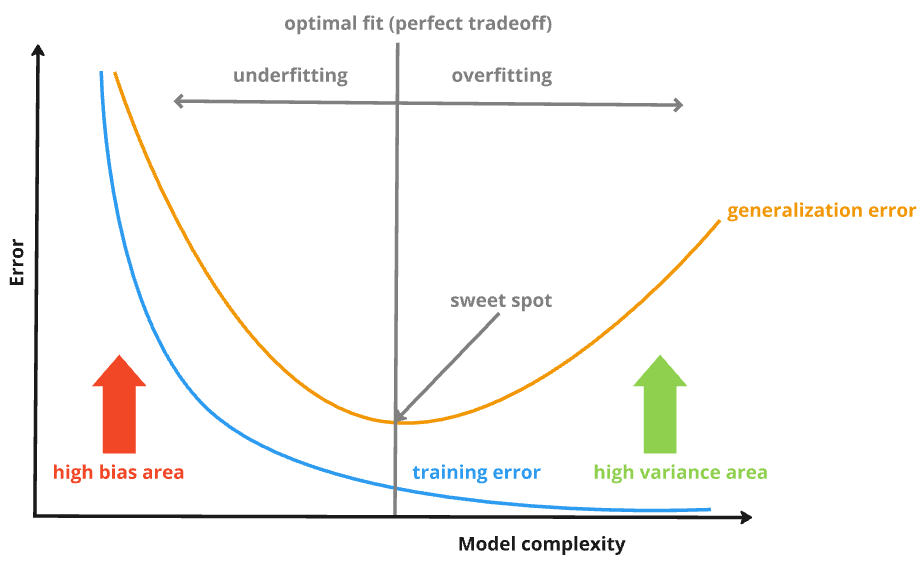
\includegraphics[width=0.8\linewidth]{img/biasvarianceunderoverfitting.png}
    \caption[Relación bias/variance con underfitting y overfitting en el contexto clásico.] {Relación bias/variance con underfitting y overfitting en el contexto clásico. Al principio, el modelo muestra un alto sesgo, incapaz de capturar adecuadamente las relaciones entre los datos. A medida que aumenta su complejidad, tanto el rendimiento en entrenamiento como en test mejora, alcanzando un punto de equilibrio en el mínimo de la curva del error de generalización (\textit{sweet spot}). Al superar este punto óptimo, el modelo comienza a memorizar los datos, lo que provoca un aumento del error de generalización, ligado a una mayor varianza. Imagen original del autor.}\label{fig:biasvarianceunderoverfitting}
\end{figure}

En definitiva, para minimizar el error de generalización en la zona clásica, es fundamental encontrar un equilibrio entre sesgo y varianza, evitando tanto el \emph{underfitting} como el \emph{overfitting}. Este equilibrio se logra mediante una elección adecuada del conjunto de hipótesis $\mathcal{H}$, el cual debe ser lo suficientemente expresivo para capturar patrones relevantes en los datos sin llegar a ser demasiado complejo para que termine modelando el ruido presente en los mismos.

\endinput


\part{Estado del Arte}
% !TeX root = ../tfg.tex
% !TeX encoding = utf8

\chapter{Trabajos relacionados}\label{sec:evolucion-ddd}

El \emph{Deep Double Descent}, al estar estrechamente relacionado al avance tecnológico y al crecimiento en la capacidad y el tamaño de los modelos de aprendizaje profundo, ha despertado un mayor interés en los últimos años, como puede observarse en la~\autoref{fig:histogram}. No obstante, aunque se percibe durante los últimos años una tendencia al alza del número de artículos que hacen referencia al mismo, únicamente encontramos un total 224 publicaciones en Scopus\footnote{Encontradas 224 publicaciones a fecha 21 de marzo de 2025 usando la consulta: TITLE-ABS-KEY ( ( deep AND double AND descent ) OR ( overparameterized AND generalization ) ) AND PUBYEAR < 2025 AND ( LIMIT-TO ( SUBJAREA,"COMP" ) OR LIMIT-TO ( SUBJAREA,"ENGI" ) OR LIMIT-TO ( SUBJAREA,"MATH" ) OR LIMIT-TO ( SUBJAREA,"PHYS" ) ) AND ( LIMIT-TO ( EXACTKEYWORD,"Machine Learning" ) OR LIMIT-TO ( EXACTKEYWORD,"Deep Learning" ) OR LIMIT-TO ( EXACTKEYWORD,"Generalization" ) OR LIMIT-TO ( EXACTKEYWORD,"Performance" ) OR LIMIT-TO ( EXACTKEYWORD,"Neural-networks" ) OR LIMIT-TO ( EXACTKEYWORD,"Deep Neural Networks" ) OR LIMIT-TO ( EXACTKEYWORD,"Overparameterization" ) OR LIMIT-TO ( EXACTKEYWORD,"Overfitting" ) OR LIMIT-TO ( EXACTKEYWORD,"Generalization Error" ) OR LIMIT-TO ( EXACTKEYWORD,"Generalization Performance" ) OR LIMIT-TO ( EXACTKEYWORD,"Neural Networks" ) OR LIMIT-TO ( EXACTKEYWORD,"Interpolation" ) OR LIMIT-TO ( EXACTKEYWORD,"Generalize" ) ).}. Esta reciente relevancia ilustra el carácter \textbf{innovador} y \textbf{pionero} de este proyecto.\newline

\begin{figure}[h]
    \centering
    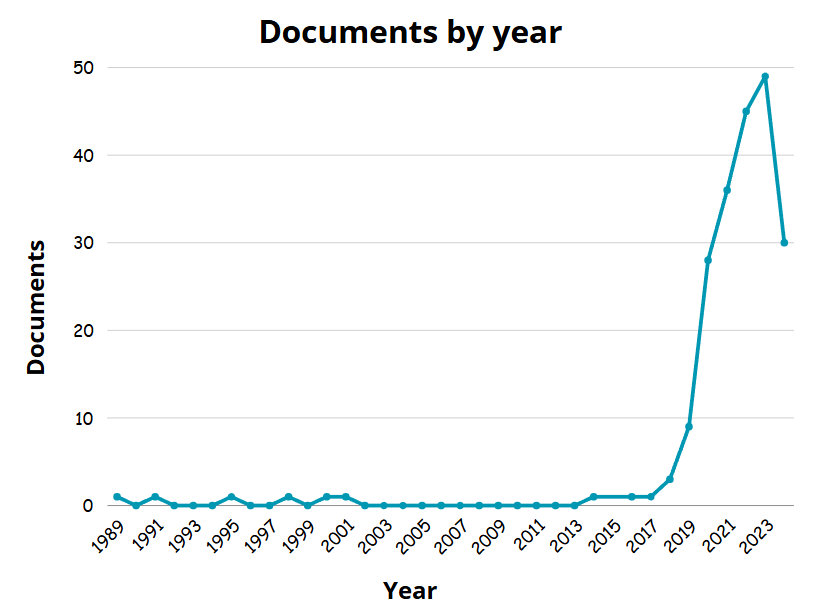
\includegraphics[width=0.8\linewidth]{img/scopus_histogram.png}
    \caption[Número de publicaciones relativas al Deep Double Descent (ir actualizando histograma de cara a nuevos papers).] {Número de publicaciones relativas al Deep Double Descent en función del año de publicación.}\label{fig:histogram}
\end{figure}

Sin embargo, aunque la cantidad de artículos científicos aún sea limitada, el interés por parte de investigadores y científicos está creciendo rápidamente. Incluso en ausencia de publicaciones científicas formales, se continúan obteniendo nuevos resultados, tanto teóricos como prácticos, que continúan enriqueciendo nuestra comprensión del problema.\newline

A pesar de la disponibilidad de artículos que abordan el tema, la mayoría de ellos no proporcionan una explicación detallada del mismo, centrándose generalmente en casos prácticos y dejando de lado el análisis teórico intrínseco, limitando la comprensión completa de ciertos aspectos y resultados.\newline

\section{Origen y primeras manifestaciones}\label{}

La primera publicación formal sobre el \emph{Deep Double Descent} data de $1989$, como se muestra en la~\autoref{fig:histogram}. En ese año, Vallet et al.~\cite{Vallet1989} presentaron, de manera empírica, este comportamiento en el ámbito de la física teórica, al emplear la pseudoinversa para abordar problemas de regresión lineal con datos artificiales. La siguiente evidencia empírica fue presentada por Krogh \& Hertz en el año $1991$~\cite{Krogh1991}, quienes, de manera parcial, mostraron el suceso utilizando un modelo de regresión lineal.\newline

Posteriormente, nos remontamos hasta $1995$ cuando Opper presenta los primeros resultados teóricos en su artículo ``Statistical Mechanics of Generalization''~\cite{Opper1995}, a través del uso de una red neuronal formada por un perceptrón de una sola capa con una función de activación lineal conocida como ADALINE~\cite{WidrowHoff1960}, y, más tarde, en su revisión del artículo en $2001$ ``Learning to Generalize''~\cite{Opper2001}.\newline

\begin{figure}[h]
    \centering
    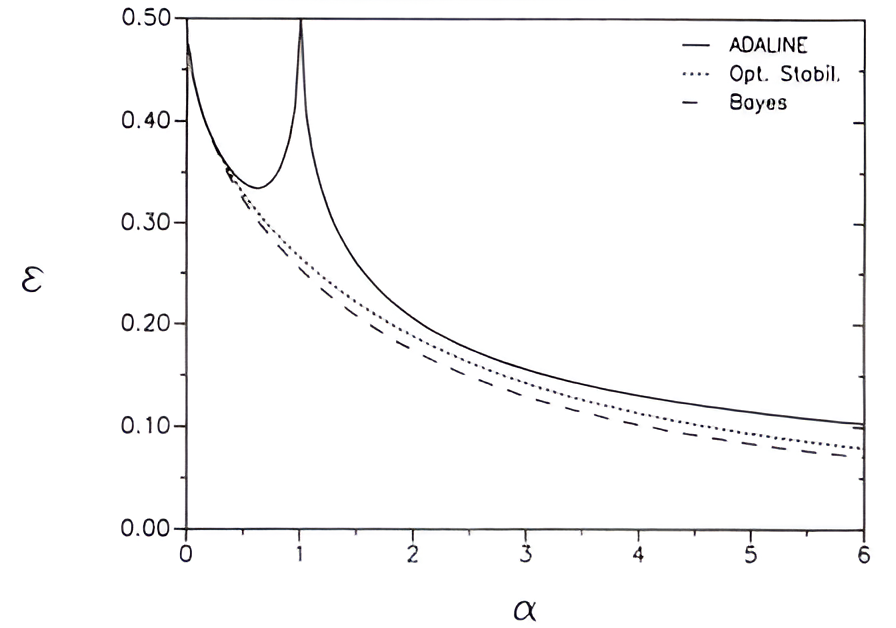
\includegraphics[width=0.8\linewidth]{img/estadoarte2.png}
    \caption[Deep Double Descent presente en ADALINE.]{Comparación del error de generalización ($\epsilon$) para distintos modelos en función de la fracción entre el número de ejemplos aprendido y el número de parámetros ($\alpha$). Se observa la curva del doble descenso para el modelo ADALINE~\cite{Opper1995}.}\label{fig:estadoarte2}
\end{figure}

En sus representaciones (véase~\autoref{fig:estadoarte2}), el error de generalización ($\epsilon$) se muestra en función del número de ejemplos de entrenamiento ($n$) y el número de parámetros ($P$), donde $\alpha = \frac{n}{P}$. Se observa que el error de generalización alcanza su máximo cuando $\alpha$ se aproxima a $1$, es decir, cuando el número de ejemplos de entrenamiento es similar al número de parámetros del modelo. En adición, demuestra que, para ciertas configuraciones, cuando $N$ tiende a infinito, la solución que proporciona la pseudoinversa mejora a medida que nos alejamos del ``pico'' $(\alpha = 1)$. \newline

Comportamientos similares a los obtenidos por Opper también han sido reportados por Advani \& Saxe en $2017$~\cite{Advani2017}, así como por Spigler et al.\ y Geiger et al.\ en $2019$~\cite{Spigler2019, Geiger2019}. Estos trabajos, anteriores a la formalización del fenómeno tal como se conoce hoy en día, trabajan con redes neuronales profundas con un gran número de parámetros y estudian el comportamiento del error de generalización utilizando herramientas de física estadística inspiradas en el trabajo de Opper. De esta manera, Spigler et al.\ y Geiger et al.\ proponen una conexión entre el doble descenso y la transición \textit{jamming} propia de la física estadística, mostrando por qué los modelos pueden llegar a generalizar mejor después del ``pico'' del error de prueba.\newline

No obstante, fue Duin en el año $2000$~\cite{Duin2000} (véanse Figuras 6 y 7) el primero en mostrar curvas de generalización utilizando datos del mundo real, bastante similares a las curvas del doble descenso que tenemos hoy en día.\newline

\section{El nacimiento del Deep Double Descent}\label{}

Iniciamos esta sección abordando el equilibrio clásico entre sesgo y varianza, un concepto fundamental en la teoría del aprendizaje automático~\cite{Geman1992, Hastie2001, Bengio2010}. Esta teoría sostiene que, a medida que la complejidad de un modelo aumenta, su sesgo disminuye, pero su varianza se incrementa. Como resultado, llega un punto en el que el error de generalización aumenta, formando la tradicional curva en forma de ``U''. De acuerdo con esta visión tradicional, una vez superado cierto umbral de complejidad, los modelos más grandes son cada vez peores y, por tanto, se busca encontrar un equilibrio en el modelo.\newline

Sin embargo, los resultados prácticos modernos no comparten esta teoría. En la actualidad, la visión moderna entre los profesionales es que los \emph{modelos grandes son mejores}~\cite{Krizhevsky2012, Neal2019, Huang2019, Szegedy2014}. Estos estudios muestran que el uso de redes neuronales con un gran número de parámetros conduce a un mejor rendimiento, evidenciando que los modelos más complejos pueden obtener resultados superiores a los modelos simples.\newline

Este trabajo se enmarca dentro del estudio de la generalización en redes neuronales profundas. En particular, se enlaza con investigaciones previas, como la de Zhang et al.\ en $2021$~\cite{Zhang2021}, quienes argumentan que comprender el aprendizaje profundo aún requiere replantearse los paradigmas tradicionales de generalización, desafiando la noción clásica de sesgo-varianza.\newline

El \emph{Deep Double Descent} fue nombrado así, por primera vez, por Belkin et al.\ en $2019$ \cite{Belkin2019}, haciendo referencia a los dos descensos que presenta la curva del error de generalización. En este artículo, se busca unificar la teoría clásica del equilibrio sesgo-varianza con los resultados prácticos obtenidos por la teoría moderna, mediante una curva de error unificada (véase~\autoref{fig:estadoarte2.2}).\newline

\begin{figure}[h]
    \centering
    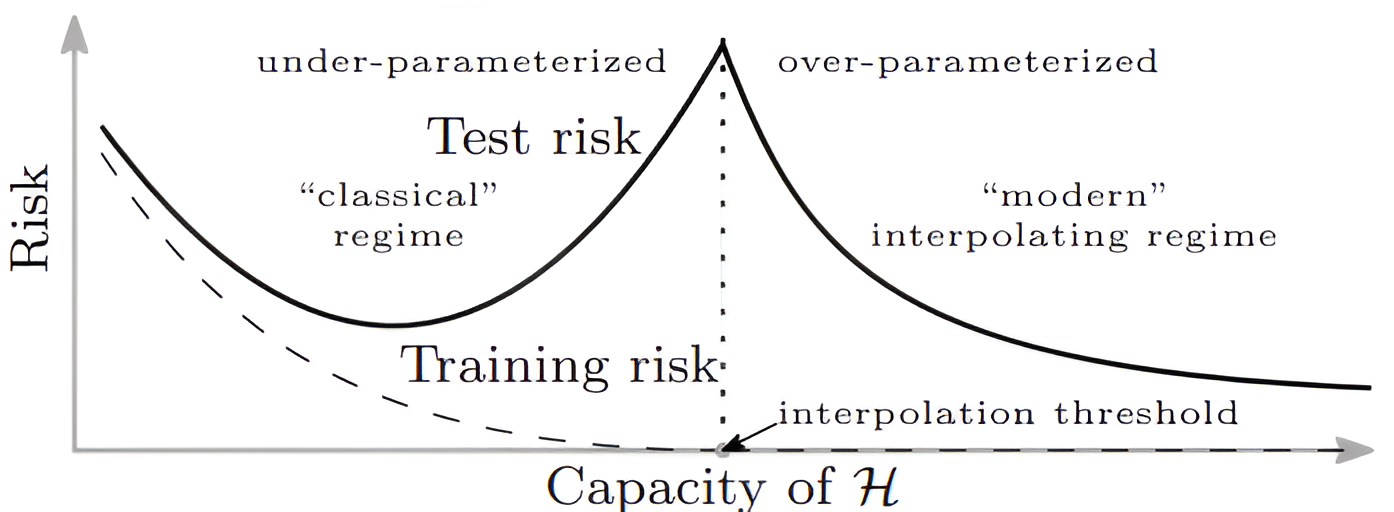
\includegraphics[width=0.8\linewidth]{img/estadoarte2.2.png}
    \caption[Curva del error unificada entre la teoría clásica y moderna~\cite{Belkin2019}.]{Curvas para el error de entrenamiento (línea discontinua) y el error de generalización (línea continua)~\cite{Belkin2019}. Antes del umbral de interpolación, se muestra la curva clásica en ``U''. Después de dicho umbral, se observa la curva del error moderna, induciendo el doble descenso.}\label{fig:estadoarte2.2}
\end{figure}

Belkin et al.\ muestran la aparición del doble descenso en diversos modelos y sobre distintos tipos de datos, entre los que se incluyen los árboles de decisión y redes neuronales poco profundas. Además, ofrece una primera intuición sobre su causa argumentando que, en la región sobreparametrizada, el modelo dispone de un mayor número de funciones candidatas compatibles con los datos. A esto se suma el efecto de la regularización implícita inducida por ciertos algoritmos de optimización, como el gradiente descendente~\cite{Soudry2024}.\newline

Posteriormente, Nakkiran et al.\ en $2019$~\cite{Nakkiran2019} observaron que el doble descenso no solo dependía del tamaño del modelo, sino también del número de épocas de entrenamiento. Además, unificaron estos resultados mediante la introducción de una nueva medida de complejidad para un modelo: la \textbf{complejidad efectiva del modelo}, y conjeturaron bajo qué condiciones podía ocurrir en función de dicha medida. En este mismo trabajo, también formalizaron los distintos tipos que pueden manifestarse: en función del número de parámetros, del número de épocas y del tamaño del conjunto de entrenamiento, los cuales constituirán la base conceptual sobre la que desarrollaremos este proyecto.\newline


\section{Avances recientes}\label{}

En los últimos años, la comprensión del \textit{Deep Double Descent} ha avanzado significativamente, con nuevas investigaciones que han refinado su caracterización y explorado sus implicaciones en redes neuronales profundas.\newline

Uno de los principales avances en el campo del aprendizaje estadístico ha sido la reconsideración de los límites de la sabiduría clásica sobre el sesgo y la varianza, especialmente al analizar el impacto del uso de un gran número de parámetros en el aprendizaje~\cite{Zhang2021,Curth2023}. Por otro lado, Schaeffer et al.\ en $2023$~\cite{Schaeffer2023} realizaron los primeros estudios teóricos y experimentales enfocados en identificar y analizar las posibles causas y factores que pueden desencadenar el fenómeno.\newline

Otras líneas de investigación han explorado cómo ciertas técnicas pueden mitigar su presencia. Por ejemplo, Yang y Suzuki en $2023$~\cite{Yang2024} analizaron el impacto de la regularización mediante el uso de dropout, demostrando que dicha técnica puede reducir la magnitud del segundo descenso en el error de generalización. Asimismo, Heckel y Yilmaz en $2021$~\cite{Heckel2020} investigaron cómo el uso de la parada anticipada \emph{o early stopping} puede influir en su aparición.\newline

Desde una perspectiva más empírica, varios estudios han analizado su manifestación en escenarios de aprendizaje adversario. En particular, Min et al. en $2021$~\cite{Ming2020} demostraron que, en algunos casos, un aumento de los datos de entrenamiento puede mejorar la robustez del modelo, aunque también puede provocar un descenso adverso en la generalización. Asimismo, Singh et al. en $2022$~\cite{Singh2022} presentaron un análisis teórico en redes neuronales de tamaño finito, proporcionando una caracterización matemática básica que ayuda a entender los mecanismos subyacentes. Por último, Somepalli et al. en $2022$~\cite{Somepalli2022} investigaron la reproducibilidad del aprendizaje en redes neuronales y su relación con el \textit{Deep Double Descent}.\newline

Finalmente, investigaciones recientes han mostrado extensiones del doble descenso, pues este no está necesariamente limitado a dos descensos, sino que, bajo ciertas circunstancias, pueden observarse más de dos descensos~\cite{d_Ascoli2021, Chen2021}. Además, se ha estudiado su relación con otros sucesos emergentes en el aprendizaje profundo, como es el caso del \emph{grokking}. En este contexto, Davies et al. en $2023$~\cite{Davies2023} propusieron una conexión entre ambos, sugiriendo que el aprendizaje prolongado puede llevar a una mejora abrupta de la generalización.\newline

Para concluir este capítulo, se presenta en la Tabla~\ref{tabla:resumen-contribuciones} un resumen de las principales publicaciones relacionadas con el doble descenso, aunque las primeras manifestaciones no utilizan la denominación actual, junto con sus contribuciones más relevantes. Asimismo, se incluye en la tabla el número de citas de cada publicación, obtenido a partir de \textit{Google Scholar}\footnote{Número de citas encontradas a día 14 de marzo de 2025.}.\newline

\begin{table}[h]
    \centering
    \small 
    \renewcommand{\arraystretch}{0.9} 
    \begin{NiceTabular}{c c c c}[hvlines,color-inside]
        \Block[fill={cyan!50}]{2-1}{\textbf{Año}} & \Block[fill={cyan!50}]{2-1}{\textbf{Referencia}} & \Block[fill={cyan!50}]{2-1}{\textbf{Principales contribuciones}} & \Block[fill={cyan!50}]{2-1}{\textbf{Citas}} \\ \\
        
        \Block{3-1}{1989} & \Block{3-1}{Vallet et al.~\cite{Vallet1989}} & \Block{3-1}{Primera manifestación empírica del suceso \\ sobre datos artificiales en la física teórica.} & \Block{3-1}{71} \\ \\ \\

        \Block{3-1}{1991} & \Block{3-1}{Krogh \& Hertz~\cite{Krogh1991}} & \Block{3-1}{Evidenciaron, parcialmente, el fenómeno en el \\ contexto de la regresión lineal.} & \Block{3-1}{2654} \\ \\ \\

        \Block{3-1}{1995} & \Block{3-1}{Manfred Opper~\cite{Opper1995}} & \Block{3-1}{Primeros resultados teóricos formales \\ sobre datos artificiales.} & \Block{3-1}{71} \\ \\ \\

        \Block{3-1}{2000} & \Block{3-1}{Robert Duin~\cite{Duin2000}} & \Block{3-1}{Primeras evidencias empíricas usando \\ datos del mundo real.} & \Block{3-1}{209} \\ \\ \\

        \Block{3-1}{2019} & \Block{3-1}{Belkin et al.~\cite{Belkin2019}} & \Block{3-1}{Unificaron la sabiduría clásica con los enfoques \\ modernos y acuñaron el nombre de \textit{Deep Double Descent}.} & \Block{3-1}{2331} \\ \\ \\

        \Block{3-1}{2019} & \Block{3-1}{Nakkiran et al.~\cite{Nakkiran2019}} & \Block{3-1}{Introdujeron la complejidad efectiva del modelo \\ y los distintos tipos de doble descenso.} & \Block{3-1}{1174} \\ \\ \\

        \Block{3-1}{2021} & \Block{3-1}{Chen et al.~\cite{Chen2021}} & \Block{3-1}{Demostraron que el error puede presentar un \\ número arbitrario de ``picos'' y que pueden controlarse.} & \Block{3-1}{80} \\ \\ \\

        \Block{3-1}{2023} & \Block{3-1}{Schaeffer et al.~\cite{Schaeffer2023}} & \Block{3-1}{Analizaron los factores que provocan su aparición \\ en modelos de regresión polinómica.} & \Block{3-1}{29} \\ \\ \\
    \end{NiceTabular}
    \caption{Resumen de los principales artículos junto con sus contribuciones.}\label{tabla:resumen-contribuciones}
\end{table}

\endinput

\part{Análisis Teórico y Empírico}
% !TeX root = ../tfg.tex
% !TeX encoding = utf8

\chapter{Análisis Teórico del Deep Double Descent}\label{ch:analisis-teorico-ddd}

En este capítulo, nos vamos a encargar de abordar, de manera teórica, el doble descenso profundo. En primer lugar, lo definiremos con la mayor precisión posible, ofreciendo una intuición clara a partir de un problema de regresión. A continuación, se presentarán los principales desarrollos presentes en la literatura científica, así como algunos avances recientes en el tema. Para concluir el capítulo, se abordará la teoría de la aproximación no lineal, ya que, a priori, presenta ciertas analogías con este fenómeno.

\section{Planteamiento teórico}\label{sec:planteamiento-teorico}

Siguiendo los resultados expuestos en la Sección~\ref{sec:subsec-underfitting-y-overfitting}, la sabiduría clásica adopta una visión en la cual sostiene que los modelos más grandes tienden a ser peores, ya que su capacidad de generalización empeora. En la práctica moderna, especialmente ahora en la era del \textit{deep learning}, es cada vez más común el uso de modelos de gran tamaño con suficientes parámetros para reducir el error de entrenamiento casi a cero. A pesar de ajustarse casi perfectamente a los datos, estos modelos logran generalizar sorprendentemente bien e incluso superar en rendimiento a modelos más simples.

De esta manera, se ha comprobado que, más allá de cierto umbral, el aumento de la capacidad de los modelos resulta beneficioso, ya que no conduce al sobreajuste y, en realidad, disminuye nuevamente el error de generalización. A esta nueva zona de funcionamiento de los modelos la denotaremos como \emph{régimen moderno} o zona sobreparametrizada, mientras que la región previa al umbral, en la que se produce la tradicional curva con forma de ``U'', la denominaremos como \textit{régimen clásico} o zona infraparametrizada.

De cara a formalizar el fenómeno del doble descenso profundo y unificar la sabiduría clásica con la práctica moderna, introducimos una nueva medida de capacidad del modelo, propuesta por Nakkiran et al.\ en~\cite{Nakkiran2019}.

\begin{definicion}[Complejidad efectiva del modelo]
    La \textbf{complejidad efectiva del modelo} (EMC, por sus siglas en inglés) de un algoritmo de aprendizaje $\mathcal{A}$, con respecto a la distribución de probabilidad conjunta $P[X, Y]$ de los datos del conjunto de entrenamiento $\mathcal{D}$, es el máximo número de ejemplos de entrenamiento $n$ en el que $\mathcal{A}$ obtiene, de media, un error de entrenamiento muy próximo a cero. Es decir, dado $\epsilon > 0$:

    \[
        EMC_{P, \epsilon}(\mathcal{A}) = \max\{ n \in \mathbb{N} \; | \; \mathbb{E}[L(g)] \leq \epsilon \},
    \]  

    donde $L(g)$ hace referencia a la función de pérdida de la función candidata $g \in \mathcal{H}$.
\end{definicion}

Una vez definida la noción de complejidad efectiva del modelo, se expone uno de los resultados principales de este trabajo.

\begin{hipotesis}\label{hipotesis-general-double-descent}
    Para cualquier distribución de datos $P[X, Y]$, algoritmo de aprendizaje basado en redes neuronales $\mathcal{A}$ (véase Subsección~\ref{subsubsec:aprendizaje-red-neuronal}) y un pequeño $\epsilon > 0$, si consideramos la tarea de predecir etiquetas basadas en $n$ muestras aleatorias e independientes de $P[X, Y]$, entonces:

    \begin{itemize}
        \item \textbf{Región infraparametrizada.} Si $EMC_{P, \epsilon}(\mathcal{A})$ es suficientemente menor que $n$, entonces cualquier perturbación de $\mathcal{A}$ que aumente su complejidad efectiva, disminuirá su error de generalización.
        \item \textbf{Región crítica.} Si $EMC_{P, \epsilon}(\mathcal{A}) \approx n$, entonces cualquier perturbación de $\mathcal{A}$ que aumente su complejidad efectiva puede aumentar o disminuir su error de generalización.
        \item \textbf{Región sobreparametrizada.} Si $EMC_{P, \epsilon}(\mathcal{A})$ es suficientemente mayor que $n$, entonces cualquier perturbación de $\mathcal{A}$ que aumente su complejidad efectiva, disminuirá su error de generalización.
    \end{itemize}
\end{hipotesis}

Esta hipótesis es informal en varios sentidos. En primer lugar, no disponemos de una forma precisa de elegir el parámetro $\epsilon$, ni de una especificación formal para ``suficientemente pequeño'' y ``suficientemente grande''. La hipótesis sugiere que hay un intervalo crítico alrededor del umbral de interpolación $(EMC_{P, \epsilon}(\mathcal{A}) = n)$ de manera que, tanto por debajo como por encima de dicho intervalo, el aumento de la complejidad beneficia el rendimiento del modelo, mientras que en el interior de este intervalo el comportamiento es incierto, pudiendo mejorar o empeorar. Además, la amplitud de dicho intervalo depende tanto de la distribución de los datos del conjunto de entrenamiento $\mathcal{D}$ como del algoritmo de aprendizaje $\mathcal{A}$ utilizado.

\begin{figure}[h]
    \centering
    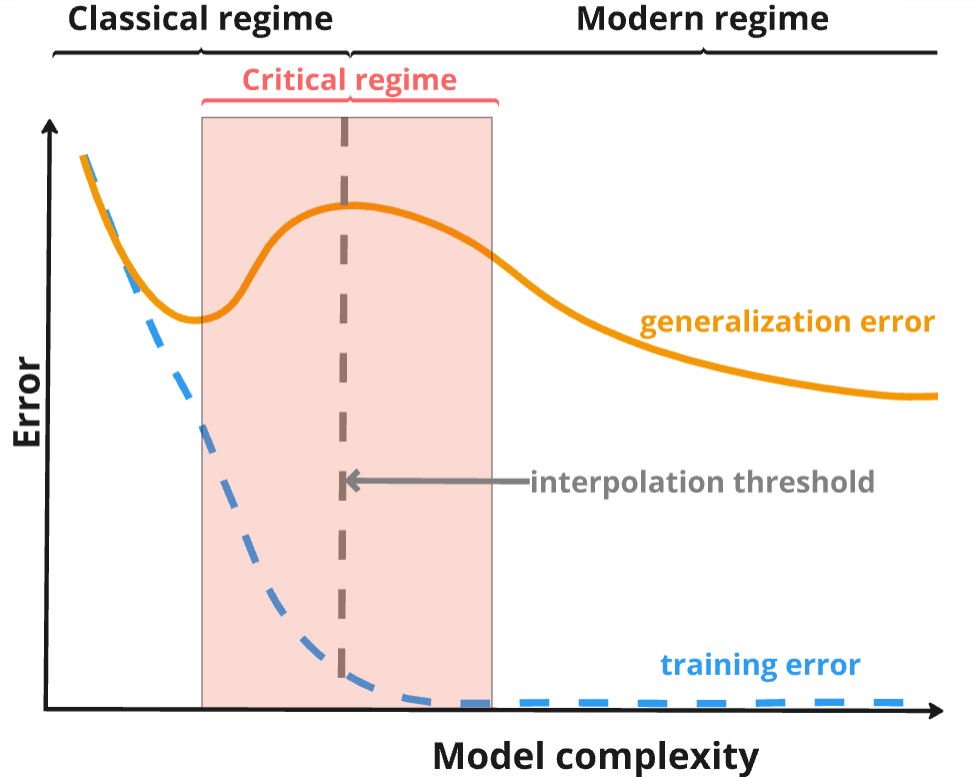
\includegraphics[width=0.6\linewidth]{img/planteamiento-teorico-dd.png}
    \caption[Ejemplo de doble descenso con las distintas zonas de parametrización.]{Ejemplo de doble descenso con las distintas zonas de parametrización. Se puede observar la tradicional forma de ``U'' en la zona clásica, seguida de la zona crítica, donde el error de generalización es incierto, ya que puede aumentar o disminuir, y, finalmente, la zona moderna, donde el error de generalización es incluso menor que el obtenido en la zona clásica.}\label{fig:planteamiento-teorico-dd.png}
\end{figure}

Por otra parte, la Hipótesis~\ref{hipotesis-general-double-descent} nos ayuda a unificar la sabiduría clásica con los resultados modernos en una curva de aprendizaje que abarca ambos mundos. Hasta el umbral de interpolación, la curva sigue la tradicional forma de ``U'', cuyo mínimo se alcanza en el \textit{sweet spot} (véase Figura~\ref{fig:biasvarianceunderoverfitting}) mientras que, aumentando la capacidad del modelo hasta alcanzar un error de entrenamiento muy próximo a cero, y tras superar la zona crítica donde se encuentra el umbral de interpolación, nos indica que el error de generalización comienza nuevamente a disminuir, pudiendo lograr un error menor que el obtenido en el \textit{sweet spot}.

Este comportamiento, en el que la curva del error de generalización exhibe dos descensos, puede apreciarse en la Figura~\ref{fig:planteamiento-teorico-dd.png} y lo denotaremos como \textbf{doble descenso profundo}, o simplemente \textbf{doble descenso}. En este contexto, el adjetivo \textit{profundo} hace referencia al uso de redes neuronales profundas como modelo base.

Aun habiendo unificado ambos puntos de vista, la descomposición del error en términos de sesgo y varianza, tal como se mencionó en la Sección~\ref{sec:capitulo-bias-variance-tradeoff}, sugiere que uno de estos dos componentes, tras alcanzar el valor máximo de error, comienza nuevamente a disminuir. La Figura~\ref{fig:bias-variance-peak} ilustra los tres comportamientos distintos que pueden surgir como resultado de dicha descomposición. Para nuestro análisis, resulta razonable suponer que es la varianza la que disminuye tras alcanzar el punto máximo del error, ya que sabemos que este término predomina a partir del \textit{sweet spot}, dando lugar a una curva unimodal.

\begin{figure}[h]
    \centering
    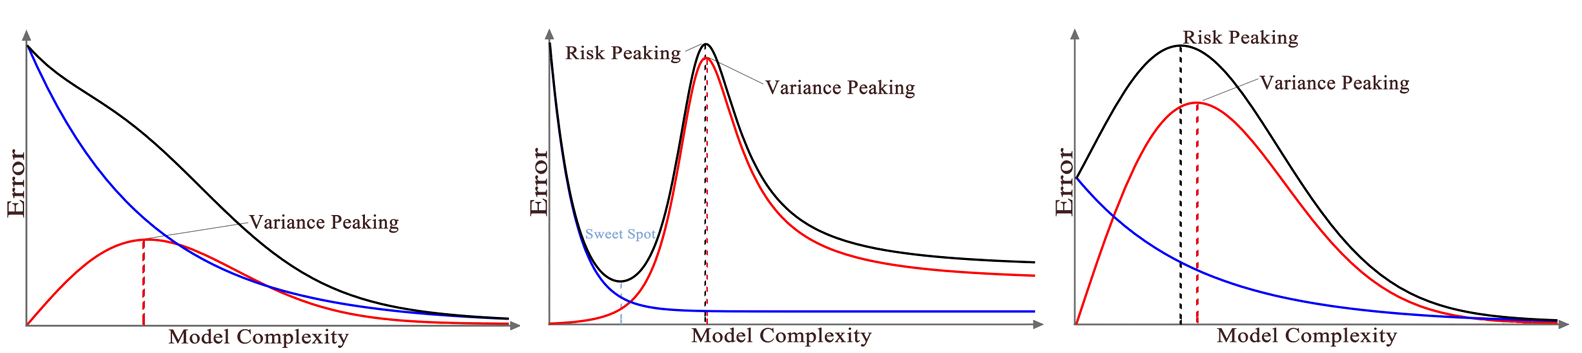
\includegraphics[width=0.9\linewidth]{img/bias-variance-peak.png}
    \caption[Curvas típicas del error en función del sesgo y la varianza~\cite{Yang2020}.]{Curvas típicas del error (línea negra) en función del sesgo (línea azul) y la varianza (línea roja)~\cite{Yang2020}. A la izquierda, el término de sesgo domina completamente, lo que da lugar a un error decreciente. En la región central, el sesgo y la varianza predominan en zonas distintas, produciéndose así el doble descenso. Finalmente, a la derecha, el término de varianza se vuelve dominante, generando una curva con forma de campana en la que el error inicialmente aumenta.}\label{fig:bias-variance-peak}
\end{figure}

De este modo, a medida que aumenta la capacidad del modelo, esto implica que, a pesar de disponer de un conjunto de hipótesis más amplio, el modelo se está concentrando en un subconjunto específico de dichas hipótesis, lo que reduce el error asociado a la varianza.

A modo de resumen, estamos separando las distintas zonas de funcionamiento de un modelo en función, en cierta medida, de su conjunto de hipótesis $\mathcal{H}$. En la zona clásica, por lo general, no existe ninguna hipótesis que minimice completamente el riesgo real, es decir, no existe $g \in \mathcal{H}$ tal que $L(g) = 0$. Por el contrario, en la zona moderna, conforme aumenta la capacidad del modelo, aparece un conjunto cada vez más amplio $S \subset \mathcal{H}$ que interpola a la perfección los datos de entrenamiento. Este conjunto se define como:  

\[
    S = \{ g \in \mathcal{H} \mid L(g) = 0 \}.
\]

En consecuencia, el verdadero problema radica en comprender por qué el algoritmo de aprendizaje $\mathcal{A}$, en la zona sobreparametrizada, tiende a seleccionar ``buenas'' soluciones dentro del conjunto $S$, es decir, aquellas que logran una buena generalización. Es importante destacar que esta cuestión no se puede responder únicamente a partir de los datos del conjunto de entrenamiento $\mathcal{D}$, ya que cualquier hipótesis de $S$ se ajusta perfectamente a esos datos. Por tanto, la clave para comprender el fenómeno vendrá dada por el sesgo inductivo que presentan algunos de los algoritmos de optimización más comunes, los cuales favorecen ciertas soluciones dentro de $S$.

\subsection{Análisis intuitivo en un problema de mínimos cuadrados}\label{subsec:analisis-intuitivo-minimos-cuadrados}

De cara a ofrecer una primera intuición sencilla sobre la ocurrencia del doble descenso, consideramos un problema de regresión lineal (basado en~\cite{Schaeffer2023}) que resolveremos utilizando el método de mínimos cuadradados ordinarios (OLS), cuya solución de norma mínima viene dada por la pseudoinversa, como vimos en la Sección~\ref{sec:svd-pseudoinversa}. Además, para comprender dónde y cómo se produce este suceso, estudiaremos las dos zonas de parametrización del modelo de regresión lineal, analizando los diferentes errores que se producen en cada una de ellas.

Supongamos que nos enfrentamos a un problema de regresión lineal en el que disponemos de $N$ ejemplos, donde cada ejemplo está formado por los respectivos datos de entrada y su correspondiente etiqueta. Sea $D$ la dimensión de los puntos de entrenamiento y $P$ el número de parámetros a ajustar para realizar la regresión lineal. De esta manera, nuestro conjunto de entrenamiento $\mathcal{D}$ está formado por $N$ pares de la forma $(x,y)$, donde $x \in \mathbb{R}^{D}$ representa un punto en el plano $D$-dimensional e $y \in \mathbb{R}$ es la variable objetivo.

Para resolver el problema de regresión lineal, debemos abordar el clásico problema de minimización de mínimos cuadrados, formulado como sigue

\begin{equation}\label{eq:minimos-cuadrados1}
    \arg\min_{w} \frac{1}{N}\sum_{n=1}^{N}\| x_n \cdot w - y_n \|^{2} = \arg\min_{w}\| Xw - Y \|^{2},
\end{equation}

donde cada par $(x, y)$ representa un ejemplo de entrenamiento y $w$ indica el vector de pesos o parámetros que queremos aprender de cara a realizar la aproximación. Además, $X \in \mathcal{M}_{N \times D}(\mathbb{R})$ y $Y\in \mathcal{M}_{N \times 1}(\mathbb{R})$ representan, respectivamente, los puntos de entrenamiento y su correspondiente salida en forma matricial.

En la zona infraparametrizada, es decir, cuando el número de ejemplos de entrenamiento es mayor que el número de parámetros a ajustar $(P < N)$, la solución al problema de minimización~\eqref{eq:minimos-cuadrados1}, ofrecida por la pseudoinversa de $X$, viene dada por ${(X^{T}X)}^{-1}X^{T}$. De este modo, el vector de pesos $w$ puede ser expresado como:

\begin{equation}
    w_{under} = {(X^{T}X)}^{-1}X^{T}Y.
\end{equation}

Por otra parte, en la zona sobreparametrizada, es decir, cuando el número de parámetros es mayor que el número de ejemplos de entrenamiento $(N < P)$, no se puede resolver el problema de minimización~\eqref{eq:minimos-cuadrados1} de manera convencional, dado que estaría mal planteado, debido al hecho de que existirían múltiples soluciones, ya que habría menos restricciones que parámetros. Por tanto, debemos seleccionar un problema de optimización distinto, que también se encuentre sujeto a las restricciones impuestas por los ejemplos de entrenamiento. En este contexto, elegimos el problema más simple que se podría imaginar, dado por:

\begin{equation}\label{eq:minimos-cuadrados2}
    \arg\min_{w}\| w \|^{2}, \quad \text{sujeto a} \; x_n \cdot w = y_n \quad \forall n \in \{1, \ldots, N\}.
\end{equation}

El problema de optimización~\eqref{eq:minimos-cuadrados2} busca el vector de parámetros con menor norma que satisface $x_n \cdot w = y_n$ para todos los ejemplos de entrenamiento. La solución a este problema de optimización también se obtiene mediante la pseudoinversa, pero en este caso, la pseudoinversa se calcula conociendo que la matriz $X$ tiene rango completo en esta región y cuenta con filas linealmente independientes. Así, la pseudoinversa viene dada por $X^{T}{(XX^{T})}^{-1}$ (véase Sección~\ref{sec:svd-pseudoinversa}). De esta forma, el vector de pesos $w$ puede ser expresado como:

\begin{equation}
    w_{over} = X^{T}{(XX^{T})}^{-1}Y.
\end{equation}

Por tanto, una vez que se ha obtenido el vector de pesos, el modelo realizará las siguientes predicciones para un determinado punto de prueba $x_{\text{test}}$, dependiendo de la zona de parametrización en la que se encuentre:

\begin{equation}
    y_{test, under} = x_{\text{test}} \cdot w_{\text{under}} = x_{\text{test}} \cdot {(X^{T}X)}^{-1}X^{T}Y.
\end{equation}

\begin{equation}
    y_{test, over} = x_{\text{test}} \cdot w_{\text{over}} = x_{\text{test}} \cdot X^{T}{(XX^{T})}^{-1}Y.
\end{equation}

No obstante y llegados a este punto, las diferencias al predecir un punto de prueba en ambas zonas de parametrización no parecen ser del todo claras. Para identificar estas diferencias con mayor precisión, reescribiremos nuestras predicciones de la siguiente forma:

\[
    y_n = x_n \cdot w^{*} + e_n,
\]

donde $w^{*} \in \mathbb{R}^{P} = \mathbb{R}^{D}$ representa el vector de parámetros ideal que realmente minimiza el error cuadrático medio y $e_n$ representa un término de error adicional presente en la propia naturaleza de los datos, es decir, un residuo que el modelo no puede capturar. Equivalentemente, en forma matricial, podemos escribir:

\[
    Y = X \cdot w^{*} + E \quad \text{con } E \in \mathbb{R}^{N \times 1}.
\]

Usando esta notación, podemos reformular las predicciones que realiza el modelo. De esta manera, para el caso de la zona infraparametrizada nos queda:

\begin{align}
    y_{test, under} &= x_{test} \cdot {(X^T X)}^{-1} X^T Y \\
    &= x_{test} \cdot {(X^T X)}^{-1} X^T (X w^{*} + E) \\
    &= x_{test} \cdot {(X^T X)}^{-1} X^T X w^{*} + x_{test} \cdot {(X^T X)}^{-1} X^T E \\
    &= \underbrace{x_{test} \cdot w^{*}}_{\overset{def}{=} y^*_{test}} + x_{test} \cdot {(X^T X)}^{-1} X^T E
\end{align}

\begin{equation}
    y_{test, under} - y^{*}_{test} = x_{test} \cdot {(X^T X)}^{-1} X^T E.
\end{equation}

Por otra parte, para el caso de la zona sobreparametrizada, los cálculos serían los siguientes:

\begin{align}
    y_{test, over} &= x_{test} \cdot X^{T}{(XX^{T})}^{-1}Y \\
    &= x_{test} \cdot X^{T}{(XX^{T})}^{-1}(X w^{*} + E) \\
    &= x_{test} \cdot X^{T}{(XX^{T})}^{-1}X w^{*} + x_{test}X^{T}{(XX^{T})}^{-1}E \\
    y_{test, over} - \underbrace{x_{test} \cdot w^{*}}_{\overset{def}{=} y^*_{test}} &= x_{test} \cdot X^{T}{(XX^{T})}^{-1}X w^{*} - x_{test} \cdot I_{D} w^{*} + x_{test} \cdot {(X^{T}X)}^{-1}X^{T}E
\end{align}

\begin{equation}
    y_{test, over} - y^{*}_{test} = x_{test} \cdot (X^{T}{(XX^{T})}^{-1}X - I_{D}) w^{*} + x_{test} \cdot {(X^{T}X)}^{-1}X^{T}E.
\end{equation}


Las ecuaciones obtenidas son importantes, aunque, a simple vista, no nos proporcionan información significativa. De cara a extraer intuiciones más claras, vamos a reemplazar la matriz $X$ por su descomposición en valores singulares (véase Sección~\ref{sec:svd-pseudoinversa}). De este modo, definimos $X = U \Sigma V^{T}$, $R = rang(X)$ y $\sigma_1 > \cdots > \sigma_R > 0$ como los valores singulares no nulos de $X$. Dado que $E \in \mathbb{R}^{N \times 1}$, podemos descomponer el error de predicción de la siguiente manera:

\begin{itemize}
    \item En la zona infraparametrizada:
        \[
            y_{test, under} - y_{test}^{*} = x_{test} \cdot V \Sigma^{\dagger} U^{T} E = \sum_{r=1}^{R}\frac{1}{\sigma_r}(x_{test} \cdot v_r)(u_r \cdot E),
        \]

        donde se ha utilizado que $V \Sigma^{\dagger} U^{T}$ corresponde a la descomposición en valores singulares de la pseudoinversa de $X$, dada por $X^{\dagger} = {(X^T X)}^{-1} X^T$.

    \item De manera análoga a la zona anterior, en la zona sobreparametrizada encontramos: 
        \[
            \begin{aligned}
                y_{test, over} - y_{test}^{*} &= x_{test} \cdot (X^{T}{(XX^{T})}^{-1}X - I_{D}) w^{*} 
                + x_{test} \cdot V \Sigma^{\dagger} U^{T} E \\
                &= x_{test} \cdot (X^{T}{(XX^{T})}^{-1}X - I_{D}) w^{*} 
                + \sum_{r=1}^{R}\frac{1}{\sigma_r}(x_{test} \cdot v_r)(u_r \cdot E),
            \end{aligned}
        \]

        donde se ha utilizado que $V \Sigma^{\dagger} U^{T}$ corresponde a la descomposición en valores singulares de la pseudoinversa de $X$, dada por $X^{\dagger} = X^{T}{(XX^{T})}^{-1}$.
\end{itemize}

LLegados a este punto, podemos analizar con mayor claridad las diferencias entre ambas predicciones. La zona sobreparametrizada incluye el término adicional $x_{test} \cdot (X^{T}{(XX^{T})}^{-1}X - I_{D}) w^{*}$, que viene a ser una proyección del punto de prueba en el espacio de características. Recordemos que, en la zona sobreparametrizada, hay más parámetros que ejemplos de entrenamiento, por lo que, para $N$ ejemplos de entrenamiento en $D = P$ dimensiones, el modelo solo puede captar fluctuaciones de los datos en $N$ dimensiones, pero no tiene visibilidad para captar las fluctuaciones en las restantes $P - N$ dimensiones.

Esto provoca la pérdida de información sobre la relación lineal óptima del vector de pesos $w^{*}$, lo que a su vez aumenta el error de predicción. Este término es el asociado al sesgo (véase Sección~\ref{sec:capitulo-bias-variance-tradeoff}), pues, al encontrarnos en la zona sobreparametrizada, disponemos de gran cantidad de hipótesis ligadas a la falta de suficientes restricciones en comparación con el número de parámetros. Esto favorece que la hipótesis ideal se encuentre dentro de ese conjunto de posibles soluciones, lo cual, a su vez, facilita que este término sea cercano a cero.

El otro término, $\sum_{r=1}^{R}\frac{1}{\sigma_r}(x_{test} \cdot v_r)(u_r \cdot E)$, representa la influencia de cada componente singular y es el causante del doble descenso en una regresión lineal resuelta mediante el método OLS. Este término se conoce como varianza y refleja el impacto de modelar las fluctuaciones de los datos en las direcciones singulares y si dicho equilibrio está correlacionado con los objetivos de regresión.

\begin{figure}[h]
    \centering
    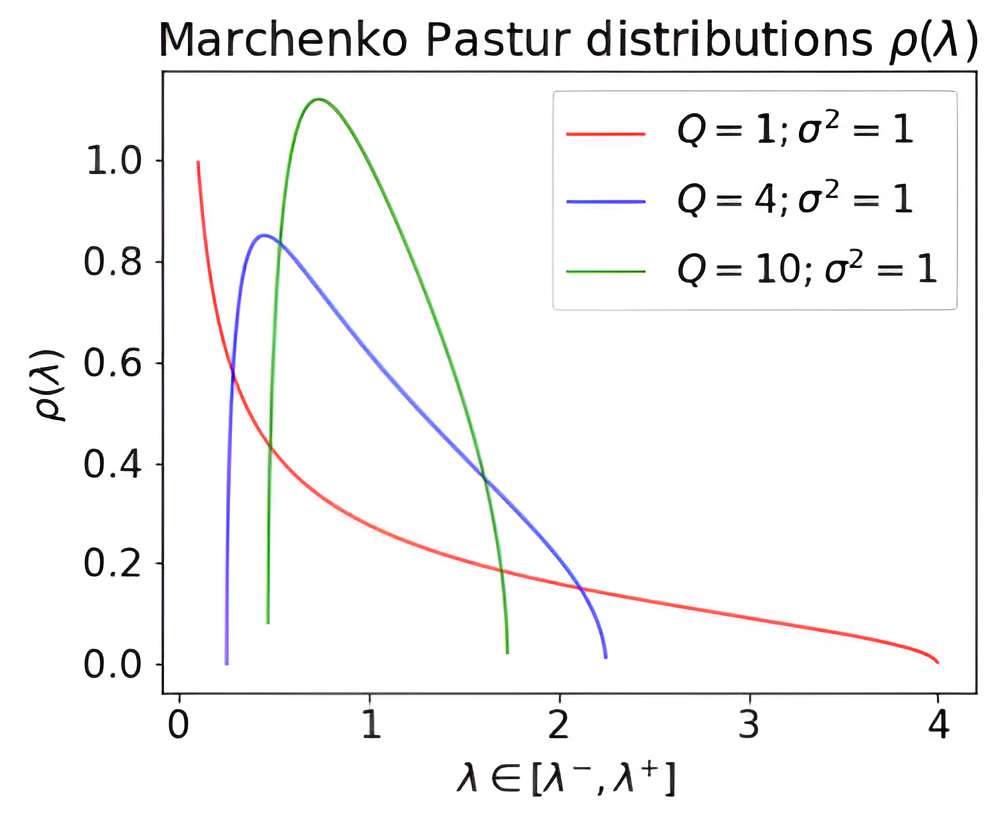
\includegraphics[width=0.5\linewidth]{img/marchenku-pastor.png}
    \caption[Ejemplos de distribuciones de Marchenko-Pastur~\cite{Charles2018}.]{Ejemplos de distribuciones de Marchenko-Pastur~\cite{Charles2018} para distintos valores de la relación de aspecto de la matriz ($Q = \frac{N}{P}$) y varianza fija. Cuando $Q = 1$, la mayoría de valores propios se acumulan alrededor del cero. A medida que $Q$ aumenta, los valores propios mínimos se alejan progresivamente de cero.}\label{fig:marchenkopastur}
\end{figure}

Por tanto, esos tres términos, multiplicados, determinan cuánto contribuye la $r$-ésima componente singular al error de predicción. Además, el ``pico'' del primer ascenso ocurre cerca del umbral de interpolación, debido a que el menor valor singular no nulo suele alcanzar su valor más bajo en dicho umbral, basado en la distribución de Marchenko-Pastur~\cite{Marchenko1967}.

A grandes rasgos, esta distribución describe el comportamiento de los valores propios de matrices aleatorias y se aplica cuando se tiene una matriz aleatoria cuyas entradas son independientes e idénticamente distribuidas, como es el caso de la matriz $X \in \mathcal{M}_{N \times D}(\mathbb{R})$. En particular, la distribución de Marchenko-Pastur describe los valores propios de la matriz de covarianza $XX^{T}$, que a su vez determinan la varianza explicada por las componentes principales del modelo. De este modo, cuando la relación $\frac{N}{P}$ se aproxima a $1$, los valores propios más pequeños se acercan a $0$ (véase Figura~\ref{fig:marchenkopastur}), provocando que los valores singulares también sean casi nulos. Esto ocurre cerca del umbral de interpolación, donde $N = P = D$, y para evitar que el $N$-ésimo dato añada un valor singular pequeño no nulo a los datos de entrenamiento, deben cumplirse dos condiciones: 

\begin{itemize}
    \item Debe haber una dimensión en la que ninguno de los datos de entrenamiento anteriores haya variado significativamente.
    \item El $N$-ésimo dato debe presentar una variación considerable en esa dimensión.
\end{itemize}

Sin embargo, este escenario es muy poco probable debido a que, en la mayoría de los casos, los datos de entrenamiento se muestrean de manera independiente a partir de variables aleatorias que son i.i.d., lo que resulta en una distribución aleatoria de los datos en todas las dimensiones. Al superar este umbral de interpolación, la varianza explicada por cada dimensión de las covariables se hace más evidente y los valores singulares no nulos más pequeños se alejan de cero, lo que reduce nuevamente el término de varianza en las predicciones, pudiendo provocar el doble descenso.

\section{Convergencia del descenso de gradiente}\label{sec:sesgo-implicito-descenso-gradiente}

En esta sección, de cara a profundizar en la intuición obtenida en la sección anterior, vamos a analizar la influencia de utilizar el descenso de gradiente como método de optimización en problemas de regresión y clasificación, dado que es uno de los métodos más utilizados para entrenar redes neuronales.

\subsection{Problema de regresión}\label{subsec:problema-regresion}
En primer lugar, nos centraremos en abordar un problema de regresión utilizando el descenso de gradiente (basándonos en~\cite{Lafon2024}), en lugar de utilizar la solución que nos ofrece el problema de mínimos cuadrados asociado. Para ello, vamos a considerar nuevamente un problema de mínimos cuadrados bajo los mismos supuestos de la sección anterior. Por tanto, suponemos que nuestro conjunto de entrenamiento $\mathcal{D}$ está formado por $N$-pares de la forma $(x, y)$, donde $x \in \mathbb{R}^{D}$ y $y \in \mathbb{R}$. Así, nuestro conjunto de entrenamiento presenta la siguiente forma:

\[
    \mathcal{D} = \{ (x_i, y_i) \in \mathbb{R}^{D} \times \mathbb{R} \}, \; i \in \{ 1, \ldots, N \}.
\]

Definimos $X \in \mathcal{M}_{N \times D}(\mathbb{R})$ como la matriz cuyas filas son los vectores $x_{i}^{T}$ e $y \in \mathbb{R}^{N}$ como el vector columna cuyos elementos son los $y_i$. Recordemos que la regla de actualización del descenso de gradiente para el vector de parámetros $w$, utilizando la función de pérdida $\mathcal{L}$ y una tasa de aprendizaje $\eta$, viene dada por:

\begin{equation}
    \mathbf{w}^{(\tau + 1)} = \mathbf{w}^{(\tau)} - \eta \nabla \mathcal{L}(\mathbf{w}).
    \label{eq:descenso-gradiente2}
\end{equation}

De manera similar a la sección anterior, consideramos el siguiente problema de optimización para resolver la regresión lineal:

\begin{equation}\label{eq:regresion-lineal-gd}
    \min_{w \in \mathbb{R}^{D}} \mathcal{L}(w) = \min_{w \in \mathbb{R}^{D}} \frac{1}{2}\| Xw - y \|^{2},
\end{equation}

donde en la ecuación~\eqref{eq:regresion-lineal-gd} se agrega el término $\frac{1}{2}$ para simplificar los cáculos de las derivadas en pasos posteriores. De esta forma, podemos enfocarnos en analizar las propiedades de la solución que encuentra el descenso de gradiente.

\begin{teorema}
    El conjunto de soluciones de un problema de mínimos cuadrados, denotado por $\mathcal{S}_{LS}$, es exactamente el siguiente:

    \[
        \mathcal{S}_{LS} = \{ X^{\dagger}y + (I_D -X^{\dagger}X)u, \; u \in \mathbb{R}^{D} \}.
    \]
\end{teorema}

\begin{proof}
    Podemos expresar el error de la ecuación~\eqref{eq:regresion-lineal-gd} de la siguiente forma: $Xw - y = Xw - XX^{\dagger}y +XX^{\dagger}y - y = Xw - XX^{\dagger}y - (I_D - XX^{\dagger})y$.

    A partir de la última ecuación, sabemos que $XX^{\dagger}y$ representa la proyección de $y$ sobre el espacio columna de $X$ y $(I_D - XX^{\dagger})y$ corresponde a su componente ortogonal. Esto se debe a que $XX^{\dagger}y$ es la proyección sobre $Im(X)$ y $(I_D - XX^{\dagger})y$ es la proyección en el complemento ortogonal de $Im(X)$, es decir, el $\ker(X^{T})$. Para verificar estas afirmaciones, basta utilizar ambas propiedades de manera conjunta en el Lema~\ref{lema:propiedades-pseudoinversa}.

    Dado que ambos términos son ortogonales, podemos descomponer la norma del error de la siguiente forma:

    \[
        \| Xw - y \|^{2} = \| Xw - XX^{\dagger}y \|^{2} + \| (I_D - XX^{\dagger})y \|^{2}
,    \]

    lo que nos lleva a la siguiente desigualdad:

    \[
        \| Xw - y \|^{2} \geq \| (I_D - XX^{\dagger})y \|^{2}.
    \]

    Finalmente, la igualdad se alcanza si y solo si:

    \[
        Xw - XX^{\dagger}y = 0 \implies  Xw = XX^{\dagger}y.
    \]

    De esta manera, sabemos que $X^{\dagger}y$ es una solución particular de la ecuación $Xw = XX^{\dagger}y$. Para obtener la solución general, basta con añadir cualquier vector que se encuentre en el núcleo de $X$, es decir, cualquier vector de la forma $\{ (I_D-X^{\dagger}X)u, \; u \in \mathbb{R}^{D} \}$ (véase Lema~\ref{lema:propiedades-pseudoinversa}).
\end{proof}

Una vez que conocemos el conjunto de soluciones para nuestro problema de optimización, podemos analizar cómo se comporta dicho conjunto en función del rango de la matriz $X$.

\begin{observacion}
    Dependiendo del rango de la matriz $X$, el conjunto de soluciones $\mathcal{S}_{LS}$ variará en función de la expresión de la pseudoinversa $X^{\dagger}$:

    \begin{itemize}
        \item Si $N < D$ y $rang(X) = N$, entonces $X^{\dagger} = X^{T}{(XX^{T})}^{-1}$ y $\mathcal{S}_{LS} = \{ X^{T}{(XX^{T})}^{-1}y + (I_D-X^{T}{(XX^{T})}^{-1}X)u, \; u \in \mathbb{R}^{D} \}$.
        
        \item Si $D < N$ y $rang(X) = D$, entonces $X^{\dagger} = {(X^{T}X)}^{-1}X^{T}$ y $\mathcal{S}_{LS} = \{ {(X^{T}X)}^{-1}X^{T}y \}$.
        
        \item Si $D = N$ y $X$ tiene inversa, entonces $X^{\dagger} = {X}^{-1}$ y $\mathcal{S}_{LS} = \{{X}^{-1}y \}$.
    \end{itemize}

    En particular, en los dos últimos casos, dado que $\ker(X)$ es trivial, la solución del problema es única.
\end{observacion}

Por tanto, nos interesa centrarnos en analizar cómo de tan buena es la solución que proporciona el descenso de gradiente en la región sobreparametrizada, es decir, cuando $N < D$, dado que es en este caso cuando se generan múltiples soluciones, mientras que en los otros casos la solución es única.

\begin{teorema}
    Si el problema de mínimos cuadrados lineales~\eqref{eq:regresion-lineal-gd} se encuentra en la región sobreparametrizada, es decir, $(N < D)$ y $rang(X) = N$, entonces, usando el descenso de gradiente con una tasa de aprendizaje constante $0 < \eta < \frac{1}{\lambda_{\max}(X)}$, donde $\lambda_{\max}(X)$ es el mayor valor propio de $X$ y partiendo desde un punto inicial $w_0 \in Im(X^{T})$, se garantiza la convergencia hacia la solución de norma mínima.
\end{teorema}

\begin{proof}
    Dado que estamos suponiendo que $X$ tiene $N$ filas linealmente independientes, podemos expresar su descomposición en valores singulares de la siguiente manera:

    \[
        X = U \Sigma V^T = \begin{bmatrix} U_1 & U_2 \end{bmatrix} \begin{bmatrix} \Sigma_1 & 0 \\ 0 & 0 \end{bmatrix} \begin{bmatrix} V_1^T \\ V_2^T \end{bmatrix},
    \]

    donde $U \in \mathbb{R}^{N \times N}$ y $V \in \mathbb{R}^{D \times D}$ son matrices ortogonales, $\Sigma \in \mathbb{R}^{N \times D}$ es una matriz diagonal rectangular, $U_1$ (respectivamente $V_1$) son las submatrices que contienen los vectores singulares izquierdos (respectivamente derechos) asociados con los valores singulares no nulos y $\Sigma_1 \in \mathbb{R}^{n \times n}$ es una matriz diagonal con valores singulares no nulos.

    Nos centramos ahora en encontrar la solución de norma mínima $w^{*}$, la cual, como sabemos, viene dada por la pseudoinversa:

    \[
        w^* = X^T {(X X^T)}^{-1} y.
    \]

    Utilizando la descomposición en valores singulares de las matrices $X$ y $X^{T}$, y dado que $V$ es ortogonal, obtenemos:

    \[
        X X^T = U \Sigma V^{T} V \Sigma^{T} U^{T} = U \Sigma \Sigma^{T} U^{T}.
    \]

    Así, para la inversa de la matriz ${(X X^T)}$, sabiendo que $U$ es ortogonal, nos queda:

    \[
        {(X X^T)}^{-1} = U {(\Sigma \Sigma^{T})}^{-1} U^{T}.
    \]

    Volviendo a usar la descomposición en valores singulares para la matriz $X^{T}$, $X^{T} = V \Sigma U^{T}$, obtenemos que la solución de norma mínima $w^{*}$ se puede reescribir como sigue (los vectores singulares asociados a los valores singulares nulos no tienen impacto en la solución de mínimos cuadrados, pues su dirección es linealmente dependiente):

    \[
        w^* = X^T {(X X^T)}^{-1} y = V \Sigma U^{T} U {(\Sigma \Sigma^{T})}^{-1} U^{T}y = V_1 \Sigma_1^{-1} U_{1}^T y.
    \]

    A continuación, trabajamos sobre la regla de actualización del gradiente descendente, que viene dada por:
    \[
        w^{(k+1)} = w^{(k)} - \eta \nabla \mathcal{L}(w) = w^{(k)} - \eta X^T (Xw^{(k)} - y) = (I - \eta X^T X)w^{(k)} + \eta X^T y,
    \]

    donde $X^T (Xw^{(k)} - y)$ hace referencia a la derivada de $\mathcal{L}(w)$ respecto de $w$.

    Seguidamente, aplicando inducción, obtenemos la expresión general:
    \[
        w^{(k)} = (I - \eta X^T X)^k w_0 + \eta \sum_{l=0}^{k-1} (I - \eta X^T X)^l X^T y.
    \]


    Ahora bien, usando la descomposición en valores singulares para la matriz $X^T X$ $(V \Sigma^T \Sigma V^T)$ y dado que $V$ es ortogonal, la iteración del gradiente descendente para el paso $k$-ésimo se expresa como:
    \[
        w^{(k)} = V (I - \eta \Sigma^T \Sigma)^k V^T w_0 + \eta V \left(\sum_{l=0}^{k-1} (I - \eta \Sigma^T \Sigma)^l \Sigma^T \right)U^T y.
    \]

    Reescribiendo la ecuación anterior en términos de $\Sigma_1$, obtenemos:
    \[
        w^{(k)} = V \begin{bmatrix} (I - \eta \Sigma_1^2)^k & 0 \\ 0 & I \end{bmatrix} V^T w_0 + \eta V \left(\sum_{l=0}^{k-1} \begin{bmatrix} (I - \eta \Sigma_1^2)^l \Sigma_1 \\ 0 \end{bmatrix} \right) U^T y.
    \]

    De cara a garantizar la convergencia del descenso de gradiente, elegimos $0 < \eta < \frac{1}{\lambda_{\max}(\Sigma_1)}$, lo que asegura que los valores propios de $I - \eta \Sigma^T \Sigma$ sean estrictamente menores que $1$, lo que implica, a su vez, que:

    \[
        \left( I - \eta \Sigma_1^T \Sigma_1 \right)^k \to 0 \quad \text{cuando} \quad k \to \infty,
    \]

    y, por tanto,

    \[
        V \begin{bmatrix} (I - \eta \Sigma_1^2)^k & 0 \\ 0 & I \end{bmatrix} V^T w_0 \xrightarrow{k \to \infty} V \begin{bmatrix} 0 & 0 \\ 0 & I \end{bmatrix} V^T w_0 = V_2 V_2^T w_0,
    \]

    dado que $V_{2}^{T}w_0$ es la parte de $w_0$ correspondiente a los valores singulares nulos de $X^{T}X$.

    Además,
    \[
        \eta \sum_{l=0}^{k-1} \begin{bmatrix} (I - \eta \Sigma_1^2)^l \Sigma_1 \\ 0 \end{bmatrix}  \xrightarrow{k \to \infty} \eta \begin{bmatrix} \sum_{l=0}^{\infty}(I - \eta \Sigma_1^2)^l \Sigma_1 \\ 0 \end{bmatrix} = \begin{bmatrix} \eta(I - I + \eta \Sigma_1^2)^{-1} \Sigma_1 \\ 0 \end{bmatrix} = \begin{bmatrix} \Sigma_1^{-1} \\ 0 \end{bmatrix}.
    \]

    Por consiguiente, denotando $w_\infty$ como el límite de las iteraciones del gradiente descendente, obtenemos:
    \[
        w_\infty = V_2 V_2^T w_0 + V_1 \Sigma_1^{-1} U^T y = V_2 V_2^T w_0 + X^{T}{(XX^{T})}^{-1}y = V_2 V_2^T w_0 + w^*.
    \]

    Finalmente, dado que $w_0$ está en la imagen de $X^T$, podemos escribir $w_0 = X^T z$ para algún $z \in \mathbb{R}^N $, lo que implica (usando la descomposición en valores singulares de la matriz $X^{T}$):
    \[
        V_2 V_2^T w_0 = V \begin{bmatrix} 0 & 0 \\ 0 & I \end{bmatrix}V^{T}X^{T}z = V \begin{bmatrix} 0 & 0 \\ 0 & I \end{bmatrix}V^{T}V\Sigma^{T}U^{T}z = V \begin{bmatrix} 0 & 0 \\ 0 & I \end{bmatrix}\begin{bmatrix} \Sigma_1 \\ 0 \end{bmatrix}U^{T}z = 0.
    \]

    En consecuencia, el término $V_2 V_2^T w_0$ desaparece, y nos queda que $w_\infty = w^{*}$, por lo que el gradiente descendente converge a la solución de norma mínima.
\end{proof}

En conclusión, tanto el gradiente descendente como la pseudoinversa llegan a la misma solución (bajo ciertas hipótesis) cuando se trata de resolver un problema de regresión lineal, ya que ambos buscan la solución interpolante de norma mínima, lo que los convierte en métodos equivalentes. De esta manera, realizar el gradiente descendente hasta la convergencia, comenzando con una inicialización de todos los pesos a cero, es equivalente a aplicar directamente la pseudoinversa. Por tanto, podemos interpretar que utilizar la pseudoinversa para resolver un problema de mínimos cuadrados es, en esencia, un caso particular del gradiente descendente aplicado al mismo problema.

\subsection{Problema de clasificación con datos separables}\label{subsec:problema-clasificación-separable}
En esta subsección, nos preocupamos de verificar el efecto de utilizar el descenso de gradiente como método de optimización en un problema de clasificación binaria con un conjunto de datos linealmente separable~\cite{Soudry2024}. Por simplicidad, condideramos un problema de clasificación binaria con un \textit{dataset} separable, lo que facilita la intuición sobre el comportamiento del descenso de gradiente. No obstante, los principios que se discuten posteriormente pueden extenderse a problemas de clasificación multiclase~\cite{Ravi2024} y al uso del descenso de gradiente en redes neuronales~\cite{Gunasekar2019}.

\begin{definicion}
    Un conjunto de datos $\mathcal{D} = \{ (x_i, y_i) \; | \; i \in \{1, \ldots, N \}\}$ donde para todo $i \in \{1, \ldots, N \}$ se verifica que $(x_i, y_i) \in \mathbb{R}^{D} \times \{-1, 1\}$, es linealmente separable si existe $w_{*} \in \mathbb{R}^{D}$ de manera que $\forall i : y_i w_{*} x_i > 0$.
\end{definicion}

Además, los resutados que se exponen en este apartado se cumplen para funciones de pérdida $\ell: \mathbb{R} \to \mathbb{R}_{+}$ que presentan las siguientes propiedades:
\begin{enumerate}
    \item\label{prop:positiva} $\ell$ es positiva, diferenciable y decreciente de manera monótona a cero $(\ell(u)>0, \ell'(u)<0 \; \text{y} \; \lim \limits_{u \to \infty} \ell(u) = \lim \limits_{u \to \infty} \ell'(u) = 0)$.
    \item\label{prop:smooth} $\ell$ es una función $\beta$-suave, es decir, el gradiente de $\ell$ es $\beta$-Lipschitz $(\forall u,v \in \mathbb{R}, \; \| \nabla \ell(u) - \nabla \ell(v) \| \leq \beta \| u-v \|)$.
    \item\label{prop:derivada_negativa} $\lim \limits_{u \to -\infty} \ell'(u) < 0$.
\end{enumerate}

Estas propiedades incluyen funciones de pérdida comunes para problemas de clasificación binaria, incluyendo la función logística y la exponencial. Además, estas propiedades implican que $\mathcal{L}(w)$ es una función $\beta \sigma^{2}_{\max}(X)$-suave (ligado al hecho de que $\ell$ es $\beta$-suave), donde $\sigma_{\max}(X)$ es el máximo valor singular de la matriz $X \in \mathbb{R}^{D \times N}$ que contiene los datos de entrenamiento.

Por tanto, para nuestro problema, consideramos un conjunto de entrenamiento $\mathcal{D}$ linealmente separable formado por $N$-pares de datos de la forma $(x_i, y_i)$ con $x_i \in \mathbb{R}^{D}$ y $y_i \in \{ -1, 1\}$, donde $i \in \{1, \ldots, N \}$ y nos centramos en minimizar la función de pérdida dada por:

\[
    \min_{w \in R^{D}}\mathcal{L}(w) = \min_{w \in R^{D}} \sum_{i=1}^{N} \ell(y_i w^{T}x_i),
\]

donde $w \in \mathbb{R}^{D}$ es el vector de parámetros y $\ell$ es una función de pérdida binaria verificando las propiedades~\ref{prop:positiva},~\ref{prop:smooth} y~\ref{prop:derivada_negativa} descritas anteriormente.

Seguidamente, nos ocupamos de estudiar la solución que ofrece el descenso de gradiente para este problema, fijada una tasa de aprendizaje $\eta$:

\[
    \mathbf{w}^{(\tau + 1)} = \mathbf{w}^{(\tau)} - \eta \nabla \mathcal{L}(\mathbf{w}) = \mathbf{w}^{(\tau)} - \eta \sum_{i=1}^{N} \ell'(y_i w^{T}x_i)y_i x_i.
\]

De cara a estudiar esta solución, utilizaremos un lema auxiliar que nos ayudará con la demostración del resultado principal de esta subsección.
\begin{lema}\label{lema:raro-clasificación-gd}
    Sea $\mathcal{L}(w)$ una función $\beta$-suave no negativa. Si $\eta < \frac{2}{\beta}$, entonces, para cualquier $w_0$ y utilizando el método del descenso de gradiente dado por:

    \[
        w^{(\tau + 1)} = w^{(\tau)} - \eta \nabla \mathcal{L}(w),
    \]

    se tiene que $\sum_{u=0}^{\infty} \| \nabla\mathcal{L}(w^{(u)}) \|^{2} < \infty$ y, por tanto:

    \[
        \lim \limits_{t \to \infty} \| \nabla\mathcal{L}(w^{(t)}) \|^{2} = 0.
    \]
\end{lema}

La demostración del lema se puede verificar en el Apéndice~\ref{ap:apendiceA}.

Una vez conocemos el resultado anterior, podemos enunciar el principal teorema de esta subsección, que establece las condiciones necesarias para que el descenso de gradiente converja hacia un punto crítico.

\begin{teorema}\label{teorema:clasificación-gd}
    Sea $\mathcal{D}$ un conjunto de entrenamiento linealmente separable con $N$ ejemplos y $\ell: \mathbb{R} \to \mathbb{R}_{+}$ una función de pérdida verificando las propiedades~\ref{prop:positiva},~\ref{prop:smooth} y~\ref{prop:derivada_negativa}. Sean $w_t$ las iteraciones del descenso de gradiente usando una tasa de aprendizaje $0 < \eta < \frac{2}{\beta \sigma^{2}_{\max}(X)}$ y cualquier punto inicial $w_0$. Entonces, se cumplen:

    \begin{enumerate}
        \item $\lim \limits_{t \to \infty} \mathcal{L}(w^{(t)}) = 0$.
        \item $\lim \limits_{t \to \infty} \| w^{(t)} \| = \infty$.
        \item $\forall i \in \{ 1, \ldotp, N\}: \; \lim \limits_{t \to \infty} y_i {w}^{(t)T} x_i = \infty$.
    \end{enumerate}
\end{teorema}

\begin{proof}
    Dado que el conjunto de entrenamiento $\mathcal{D}$ es linealmente separable, $\exists w_{*} \in \mathbb{R}^{D}$ de manera que $\forall i \in \{1, \ldots, N \} : y_i w_{*} x_i > 0$ y, entonces

    \[
        w_{*}^{T}\nabla\mathcal{L}(w) = \sum_{i=1}^{N} \underbrace{\ell'(y_i w^{T} x_i)}_{< 0} \underbrace{y_i w_{*}^{T}x_i}_{> 0} < 0.
    \]

    Para cualquier $w$ finito, la suma anterior no puede ser igual a $0$, ya que es una suma de términos negativos $(\forall i: y_i w_{*}^{T}x_i > 0)$ y $\forall u: \ell'(u) < 0$, debido a las propiedades que cumple la función de pérdida $\ell$. Por lo tanto, no hay puntos críticos finitos $w$ para los cuales $\nabla \mathcal{L}(w) = 0$. Sin embargo, el descenso de gradiente en una función de pérdida suave con una tasa de aprendizaje adecuada siempre garantiza converger a un punto crítico, es decir, $\nabla \mathcal{L}(w^{(t)}) \to 0$ (véase Lema~\ref{lema:raro-clasificación-gd}).
    
    Este hecho implica necesariamente que $\| w^{(t)} \| \to \infty$, que es la condición \textbf{($\boldsymbol{2}$)}, mientras se verifique que $\exists t_0 : \; \forall t > t_0, \; \forall i: y_i w_{t}^{T} x_i > 0$, que es la condición \textbf{($\boldsymbol{3}$)}, pues únicamente entonces se cumple $\ell'(y_i {w}^{(t)T} x_i) \to 0$. Entonces, se verifica que $\mathcal{L}(w^{(t)}) \to 0$ (condición \textbf{($\boldsymbol{1}$)}) y, por tanto, el descenso de gradiente converge hacia un mínimo global.
\end{proof}

El Teorema~\ref{teorema:clasificación-gd} nos asegura que el descenso de gradiente, eligiendo una tasa de aprendizaje adecuada, converge hacia un mínimo global, dado que $\mathcal{L}(w^{(t)}) \to 0$. Además, no se requiere que la función de pérdida $\mathcal{L}(w)$ sea convexa, lo que amplia la aplicabilidad del resultado a una clase más general de funciones.

\section{Optimización en la zona sobreparametrizada}\label{sec:optimizacion-zona-sobreparametrizada}
Como hemos observado en secciones anteriores, la sobreparametrización resulta beneficiosa dentro del marco del aprendizaje estadístico. Este comportamiento, aunque contraintuitivo: ``\textit{Un modelo con cero error de entrenamiento está por encima de los datos de entrenamiento y, por lo general, generalizará mal}''~\cite{Hastie2001}, refleja cómo las soluciones de los sistemas sobreparametrizados pueden mejorar la generalización. Sin embargo, desde el punto de vista de la optimización, que se concentra en los algoritmos y técnicas utilizadas para encontrar el mejor modelo posible, la sobreparametrización también ofrece ventajas, ya que facilita la convergencia de los métodos de optimización hacia un mínimo global, especialmente en aquellos que emplean el descenso de gradiente o alguna extensión del mismo.

En el caso de que nuestra función de pérdida $\ell: \mathcal{Y} \to \mathbb{R}$ sea convexa y nuestro modelo $g: \mathcal{X} \to \mathcal{Y}$, elegido del conjunto de hipótesis, sea lineal, es fácil observar que $l \circ f$ es convexa (basta con aplicar las propiedades de la linealidad de $g$ junto con las propiedades de convexidad de $\ell$). Como resultado, se garantiza la convergencia hacia la mejor solución, es decir, el mínimo global de la función de pérdida, sin riesgo de quedar atrapados en mínimos locales.

No obstante, en el marco del aprendizaje profundo, el modelo resultante es no lineal debido al uso de funciones de activación no lineales, lo que provoca que, en general, el paisaje de la función de pérdida sea no convexo. Esto implica que los métodos de optimización de primer orden, como el GD, puedan quedar atrapados en mínimos locales, ya que solo utilizan información local del gradiente, dependiendo así de su inicialización. Como resultado, los sistemas sobreparametrizados dan lugar a paisajes de la función de pérdida que son \textit{esencialmente no convexos}, es decir, por lo general no existe un vecindario alrededor de ningún minimizador global en el que el paisaje de la función de pérdida sea convexo. Esto contrasta con lo que ocurre en los sistemas infraparametrizados, donde dicho vecindario suele existir, aunque sea extremadamente pequeño (véase Figura~\ref{fig:localglobalminima}).

\begin{figure}[h]
    \centering
    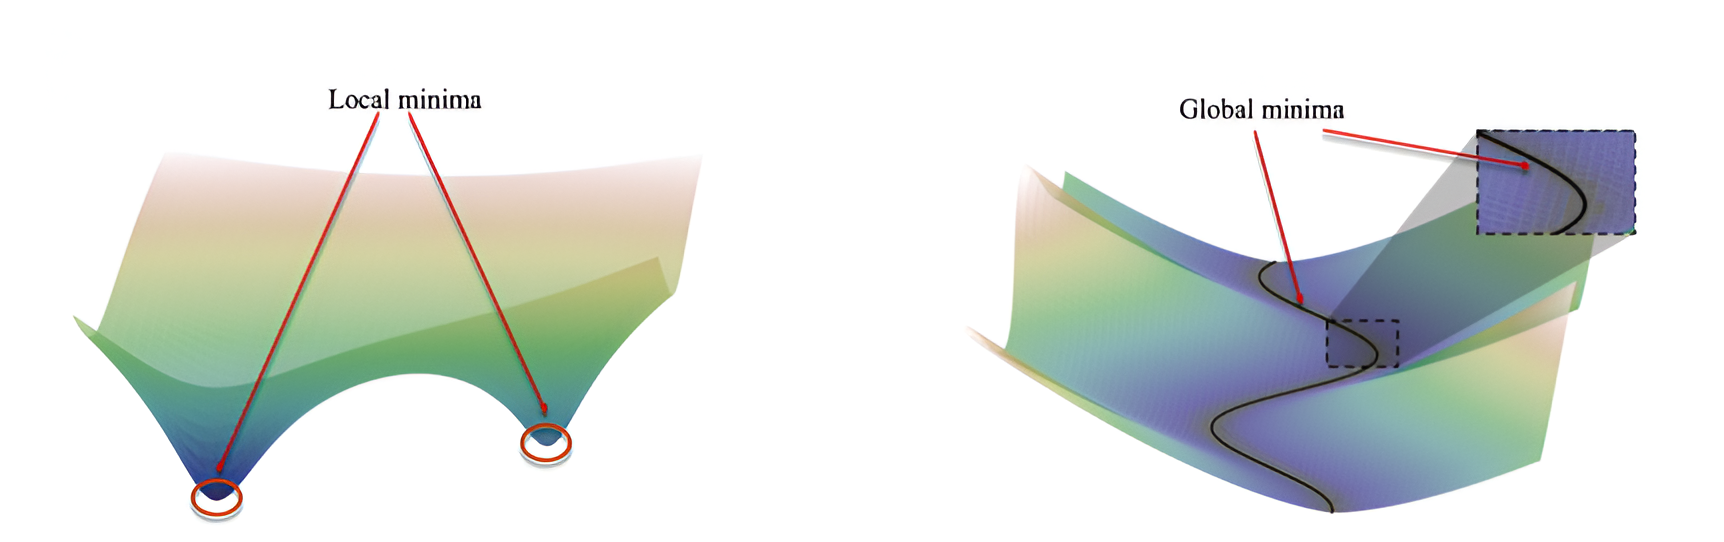
\includegraphics[width=0.8\linewidth]{img/localglobalminima.png}
    \caption[Ejemplos de paisajes de la función de pérdida en redes neuronales~\cite{Liu2021}.]{Ejemplos de paisajes de la función de pérdida en redes neuronales~\cite{Liu2021}. A la izquierda, se muestra un paisaje localmente convexo alrededor de los mínimos locales, ligado a la zona infraparametrizada. A la derecha, se muestra un paisaje incompatible con la convexidad local con múltiples mínimos globales, ligado a la zona sobreparametrizada.}\label{fig:localglobalminima}
\end{figure}

Con el fin de estudiar de manera más formal los resultados presentados, consideramos nuevamente un problema típico del aprendizaje supervisado, con un dataset $\mathcal{D}$ compuesto por $N$-pares de ejemplos de entrenamiento, es decir,  $\mathcal{D} = \{(x_i, y_i)\}_{1}^{N}$, con $x_i \in \mathbb{R}^{D}$ e $y \in \mathbb{R}$. Si consideramos nuestro conjunto de hipótesis $\mathcal{H}$ como una familia paramétrica de modelos, como, por ejemplo, una red neuronal, nuestro objetivo es encontrar el vector de parámetros óptimo $w^{*}$, de manera que el modelo se ajuste a los datos de entrenamiento, es decir

\[
    f(w^{*}; x_i) \approx y_i, \quad i \in \{1,\ldots,n \}.
\]

Matemáticamente, esto es equivalente a resolver un sistema con $N$ ecuaciones\footnote{Para problemas de clasificación multiclase o problemas de regresión con múltiples salidas, donde $C$ es el número de clases o salidas distintas, estaremos resolviendo un sistema de $N \times C$ ecuaciones.}. Agregándolas todas en una única función, podemos escribir:

\begin{equation}\label{eq:optimizacion-uno}
    \mathcal{F}(w) = y, \; \text{donde} \; w \in \mathbb{R}^{P}, y \in \mathbb{R}^{N}, \mathcal{F}(\cdot):\mathbb{R}^{P} \to \mathbb{R}^{N}.
\end{equation}

De esta manera, $(\mathcal{F}(w)) = f(w; x_i)$. Una solución exacta de la ecuación~\eqref{eq:optimizacion-uno} corresponde a la interpolación.

Usamos $\mathcal{DF}$ para representar la derivada de la función $\mathcal{F}$, donde $\mathcal{DF} \in \mathcal{M}_{N \times P}(\mathbb{R})$, con $(\mathcal{DF})_{ij} = \frac{\partial \mathcal{F}_{i}}{\partial w_j}$. Denotamos la matriz hessiana de la función $\mathcal{F}$ como $H_{\mathcal{F}}$, que es un tensor de tamaño $N \times P \times P$ con $(H_{\mathcal{F}})_{ijk} = \frac{\partial^2 \mathcal{F}_{i}}{\partial w_j \partial w_k}$, y definimos la norma del tensor hessiano como $\| H_{\mathcal{F}} \| = \max_{i \in \{1, \ldots,N \}} \| H_{\mathcal{F}_{i}} \|$, donde $H_{\mathcal{F}_{i}} = \frac{\partial^2 \mathcal{F}_{i}}{\partial w^2}$. De manera análoga, denotamos la matriz hessiana de la función de pérdida como $H_{\mathcal{L}} = \frac{\partial^2 \mathcal{L}}{\partial w^2}$.

Para detallar de manera analítica la no convexidad en la zona sobreparametrizada, se presenta el siguiente resultado.

\begin{proposicion}\label{prop:non-conexity}
    Sea $w^{*}$ una solución al problema planteado, es decir, $\mathcal{L}(w^{*}) = 0$, y supongamos que $\frac{d}{dw}\frac{\partial \mathcal{L}}{\partial \mathcal{F}}(w^{*}) \neq 0$ y $rang(H_{\mathcal{F}_{i}}(w^{*})) > 2N$ para algún $i \in \{1, \ldots, N \}$. Entonces $\mathcal{L}(w)$ no es convexa en ningún entorno de $w^{*}$.
\end{proposicion}

\begin{proof}
    Se presenta una idea intuitiva de cómo realizar la demostración del resultado anterior. Para ello, tomaremos dos puntos distintos del entorno de la solución $w^*$ y evaluaremos las matrices hessianas de la función de pérdida en dichos puntos. Una vez evaluadas, podemos verificar que ambas matrices no pueden ser negativas de manera simultánea, lo que implica que la función de pérdida $\mathcal{L}(w)$ no es localmente convexa alrededor de $w^*$, ya que la hessiana no es semidefinida positiva en ese entorno, lo cual es una condición necesaria para que la función sea localmente convexa.

    Por último, se referencia al lector más curioso al Apéndice~\ref{ap:apendiceA} para la demostración detallada de la proposición.
\end{proof}

Para el caso de sistemas infraparametrizados, los mínimos locales se encuentran generalmente aislados. Dado que $H_{\mathcal{L}}(w^{*})$ es definida positiva cuando $w^{*}$ es un mínimo aislado, por la continuidad de $H_{\mathcal{L}}(\cdot)$, la definición de positividad se preserva en el entorno de $w^{*}$. Por consiguiente, $\mathcal{L}(w)$ es localmente convexa alrededor de $w^{*}$.

A su vez, en los sistemas sobreparametrizados contamos con más parámetros que constantes. En este caso, el sistema de ecuaciones general tiene múltiples soluciones exactas, las cuales forman una variedad continua de dimensión $P - N > 0$, de modo que ninguna de estas soluciones está aislada. Este hecho puede observarse en la Figura~\ref{fig:localglobalminima} y se encuentra demostrado en el Apéndice A de~\cite{Liu2021}. En cuanto a nuestro interés, podemos concluir que, para redes suficientemente parametrizadas, los mínimos globales siempre están rodeados por otro mínimo global en un entorno relativamente pequeño.

Estos resultados nos conducen a la conclusión de que, para el análisis de los sistemas sobreparametrizados, no podemos utilizar la convexidad, ni siquiera localmente, como base. En consecuencia, es necesario buscar una condición, a priori, más simple, que verifiquen las funciones de pérdida con el fin de analizar el comportamiento de dichos sistemas. Para ello, se recurre a una modificación de la condición de Polyak y Lojasiewicz.

\begin{definicion}[Condición $\mu$-$PL$]
    Decimos que una función no negativa $\mathcal{L}$ verifica la condición $\mu$-$PL$ (Polyak-Lojasiewicz) en un conjunto $\mathcal{S} \subset \mathbb{R}^{P}$ para $\mu > 0$, si

    \[
        \| \nabla \mathcal{L}(w) \|^{2} \geq \mu \mathcal{L}(w), \; \forall w \in \mathcal{S}.
    \]
\end{definicion}

\begin{teorema}
    Supongamos que la función de pérdida $\mathcal{L}(w)$ es $\beta$-suave y cumple la condición $\mu$-$PL$ en la bola $B(w_0, R) = \{ w \in \mathbb{R}^{P} : \| w - w_0 \| \leq R \}$ con $R = \frac{2 \sqrt{2 \beta \mathcal{L}(w_0)}}{\mu}$. Entonces se tiene:

    \begin{enumerate}
        \item (\textbf{Existencia de una solución}). Existe una solución (minimizador global de $\mathcal{L}$) $w^{*} \in B(w_0, R)$, de manera que $\mathcal{F}(w^{*}) = y$.
        \item (\textbf{Convergencia del GD}). El gradiente descendente con un learning rate $\eta \leq \frac{1}{\sup_{w \in B(w_0, R)} \| \mathcal{H}_{\mathcal{L}}(w) \|}$ converge a una solución global en $B(w_0, R)$:
        \[
            \mathcal{L}(w_{t}) \leq (1 - \eta \mu)^{t} \mathcal{L}(w_0).
        \]
    \end{enumerate}
\end{teorema}

\begin{proof}
    Probaremos este teorema por inducción, sabiendo que nuestra hipótesis de inducción nos dice que, para todo $t \geq 0$, $w_t$ está dentro de la bola $B(w_0, R)$ con $R = \frac{2\sqrt{2\beta \mathcal{L}(w_0)}}{\mu}$, y $\mathcal{L}(w_t) \leq (1 - \eta \mu)^{t} \mathcal{L}(w_0)$.

    En el caso inicial, cuando $t = 0$, es trivial que $w_0 \in B(w_0, R)$ y que $\mathcal{L}(w_t) \leq (1 - \eta \mu)^{0} \mathcal{L}(w_0)$. Supongamos que, por inducción, para un $t \geq 0$, $w_t$ está en la bola $B(w_0, R)$. Para probar que $w_{t+1} \in B(w_0, R)$, usamos que la función de pérdida $\mathcal{L}$ es $\beta$-suave y, por tanto, verifica:

    \begin{equation}\label{eq:solucioinduccion1}
        \mathcal{L}(w_{t+1}) - \mathcal{L}(w_{t}) - \nabla \mathcal{L}(w_{t}) (w_{t+1} - w_{t}) \leq \frac{\beta}{2} \| w_{t+1} - w_{t} \|^2.
    \end{equation}

    Tomando $w_{t+1} - w_{t} = -\eta \nabla \mathcal{L}(w_{t})$ en la ecuación~\eqref{eq:solucioinduccion1}, nos queda:  

    \begin{equation}\label{eq:solucioinduccion2}
        \mathcal{L}(w_{t+1}) - \mathcal{L}(w_{t}) + \eta \| \nabla \mathcal{L}(w_{t}) \|^2 \leq \frac{\beta}{2} \eta^2 \| \nabla \mathcal{L}(w_{t}) \|^2,
    \end{equation}

    lo que implica que

    \begin{equation}\label{eq:solucioinduccion3}
        \mathcal{L}(w_{t+1}) - \mathcal{L}(w_{t}) \leq - \left( \eta - \frac{\beta}{2}\eta^2 \right) \| \nabla \mathcal{L}(w_{t}) \|^2.
    \end{equation}

    Además, usando el Lema~\ref{lema:raro-clasificación-gd} para $\eta \leq \frac{1}{\beta}$, se verifica

    \begin{equation}\label{eq:solucioinduccion4}
        \mathcal{L}(w_{t+1}) - \mathcal{L}(w_{t}) \leq - \frac{\eta}{2} \| \nabla \mathcal{L}(w_{t}) \|^2 \implies \frac{2(\mathcal{L}(w_{t}) - \mathcal{L}(w_{t+1}))}{\mu} \geq \| \nabla \mathcal{L}(w_{t}) \|^2.
    \end{equation}

    Aplicando la condición $\mu$-PL a la primera parte de la ecuación anterior, se satisface

    \begin{equation}\label{eq:solucioinduccion5}
        - \frac{\eta}{2} \| \nabla \mathcal{L}(w_{t}) \|^2 \leq -\eta \mu \mathcal{L}(w_{t}).
    \end{equation}

    Finalmente, por la hipótesis de inducción, se cumple

    \begin{equation}\label{eq:solucioinduccion6}
        \mathcal{L}(w_{t+1}) \leq (1 - \eta \mu)\mathcal{L}(w_{t}) \leq (1 - \eta \mu)^{t+1}\mathcal{L}(w_0).
    \end{equation}

    Ahora, podemos analizar la distancia de $w_{t+1}$ a $w_0$:

    \begin{align}
        \| w_{t+1} - w_0 \| &= \eta \bigg\| \sum_{i=0}^{t} \nabla \mathcal{L}(w_i) \bigg\| \leq \eta \sum_{i=0}^{t} \| \nabla \mathcal{L}(w_i) \| \\
        &\leq \eta \sum_{i=0}^{t} \sqrt{2 \beta (\mathcal{L}(w_i) - \mathcal{L}(w_{i+1}))} \quad \text{(usando $\eta = \frac{1}{\beta}$ en la ecuación~\eqref{eq:solucioinduccion4})} \\
        &\leq \eta \sum_{i=0}^{t} \sqrt{2 \beta \mathcal{L}(w_i)} \\
        &\leq \eta \sqrt{2\beta} \left( \sum_{i=0}^{t} (1 - \eta \mu)^{i/2} \right) \sqrt{\mathcal{L}(w_0)} \quad \text{(usando la ecuación~\eqref{eq:solucioinduccion5})} \\
        &\leq \eta \sqrt{2\beta} \sqrt{\mathcal{L}(w_0)} \frac{1}{1 - \sqrt{1 - \eta \mu}} \leq \frac{2 \sqrt{2\beta} \sqrt{\mathcal{L}(w_0)}}{\mu} = R.
    \end{align}

    Por tanto, $w_{t+1}$ se encuentra en la bola $B(w_0, R)$.
\end{proof}

Finalmente, se presenta una idea intuitiva, utilizando la función de pérdida cuadrática, de por qué los paisajes de pérdida de los sistemas sobreparametrizados satisfacen la condición $\mu$-PL en la mayor parte de su espacio de parámetros.

\begin{definicion}
    El núcleo tangente de la función $\mathcal{F}$ en el vector $w$ se define como

    \[
        K(w) = \mathcal{DF}(w)\mathcal{DF}^{T}(w),
    \]

    y, entonces, $K(w) \in \mathcal{M}_{N \times P}(\mathbb{R})$ es una matriz semidefinida positiva.
\end{definicion}

\begin{definicion}[Condicionamiento uniforme]
    Decimos que $\mathcal{F}(w)$ está $\mu$-uniformemente condicionada $(\mu > 0)$ en un subconjunto $\mathcal{S} \subset \mathbb{R}^{P}$ si el valor propio más pequeño de su núcleo tangente satisface

    \[
        \lambda_{\min}(K(w)) \geq \mu, \; \forall w \in \mathcal{S}.
    \]
\end{definicion}

El siguiente resultado muestra cómo el hecho de estar condicionada de manera uniforme es una condición suficiente para que la pérdida cuadrática cumpla la condición $\mu$-PL.

\begin{teorema}[Condicionamiento uniforme $\implies$ Condición $\mu$-PL]
    Si $\mathcal{F}(w)$ está $\mu$-uniformemente condicionada en un conjunto $\mathcal{S} \subset \mathbb{R}^P$, entonces la función de pérdida cuadrática $\mathcal{L}(w) = \frac{1}{2} \|\mathcal{F}(w) - y \|^2$ satisface la condición $\mu$-PL$^*$ en $\mathcal{S}$.
\end{teorema}

\begin{proof}
    \[
        \begin{aligned}
            \frac{1}{2} \|\nabla \mathcal{L}(w)\|^2 &= \frac{1}{2} (\mathcal{F}(w) - y)^T K(w) (\mathcal{F}(w) - y) \\
            &\geq \frac{1}{2} \lambda_{\min}(K(w)) \|\mathcal{F}(w) - y \|^2 = \lambda_{\min}(K(w)) \mathcal{L}(w) \geq \mu \mathcal{L}(w).
        \end{aligned}
    \]

\end{proof}

Nos centramos ahora en mostrar una intuición de por qué la pérdida cuadrática cumple la condición $\mu$-PL en la mayor parte del espacio de parámetros. La observación clave viene dada por el rango del núcleo tangente:

\[
        rang(K(w)) = rang((\mathcal{DF}(w) \mathcal{DF}^T(w))) = rang(\mathcal{DF}(w)),
\]

donde $K(w)$ es, por definición, una matriz semidefinida positiva. Por tanto, el conjunto singular $\mathcal{S}_{\text{sing}}$, donde el núcleo tangente es degenerado, se puede escribir como

\[
    \mathcal{S}_{\text{sing}} = \{w \in \mathbb{R}^P \mid \lambda_{\min}(K(w)) = 0\} = \{w \in \mathbb{R}^P \mid rang(\mathcal{DF}(w)) < n\}.
\]

Así, tenemos que $rang(K(w)) = \min(P, N)$. Para el caso más simple, consideremos $N = 1$. En este caso, el núcleo tangente es un escalar y $K(w) = \| \mathcal{DF}(w) \|^2$ es singular si y solo si $\mathcal{DF}(w) = 0$. Como resultado, mediante un análisis de conteo de parámetros, esperamos que el conjunto singular $\mathcal{S}_{\text{sing}} = \{ w \mid K(w) = 0 \}$ tenga codimensión $P$ y, en consecuencia, consista únicamente de puntos aislados.

\begin{figure}[h]
    \centering
    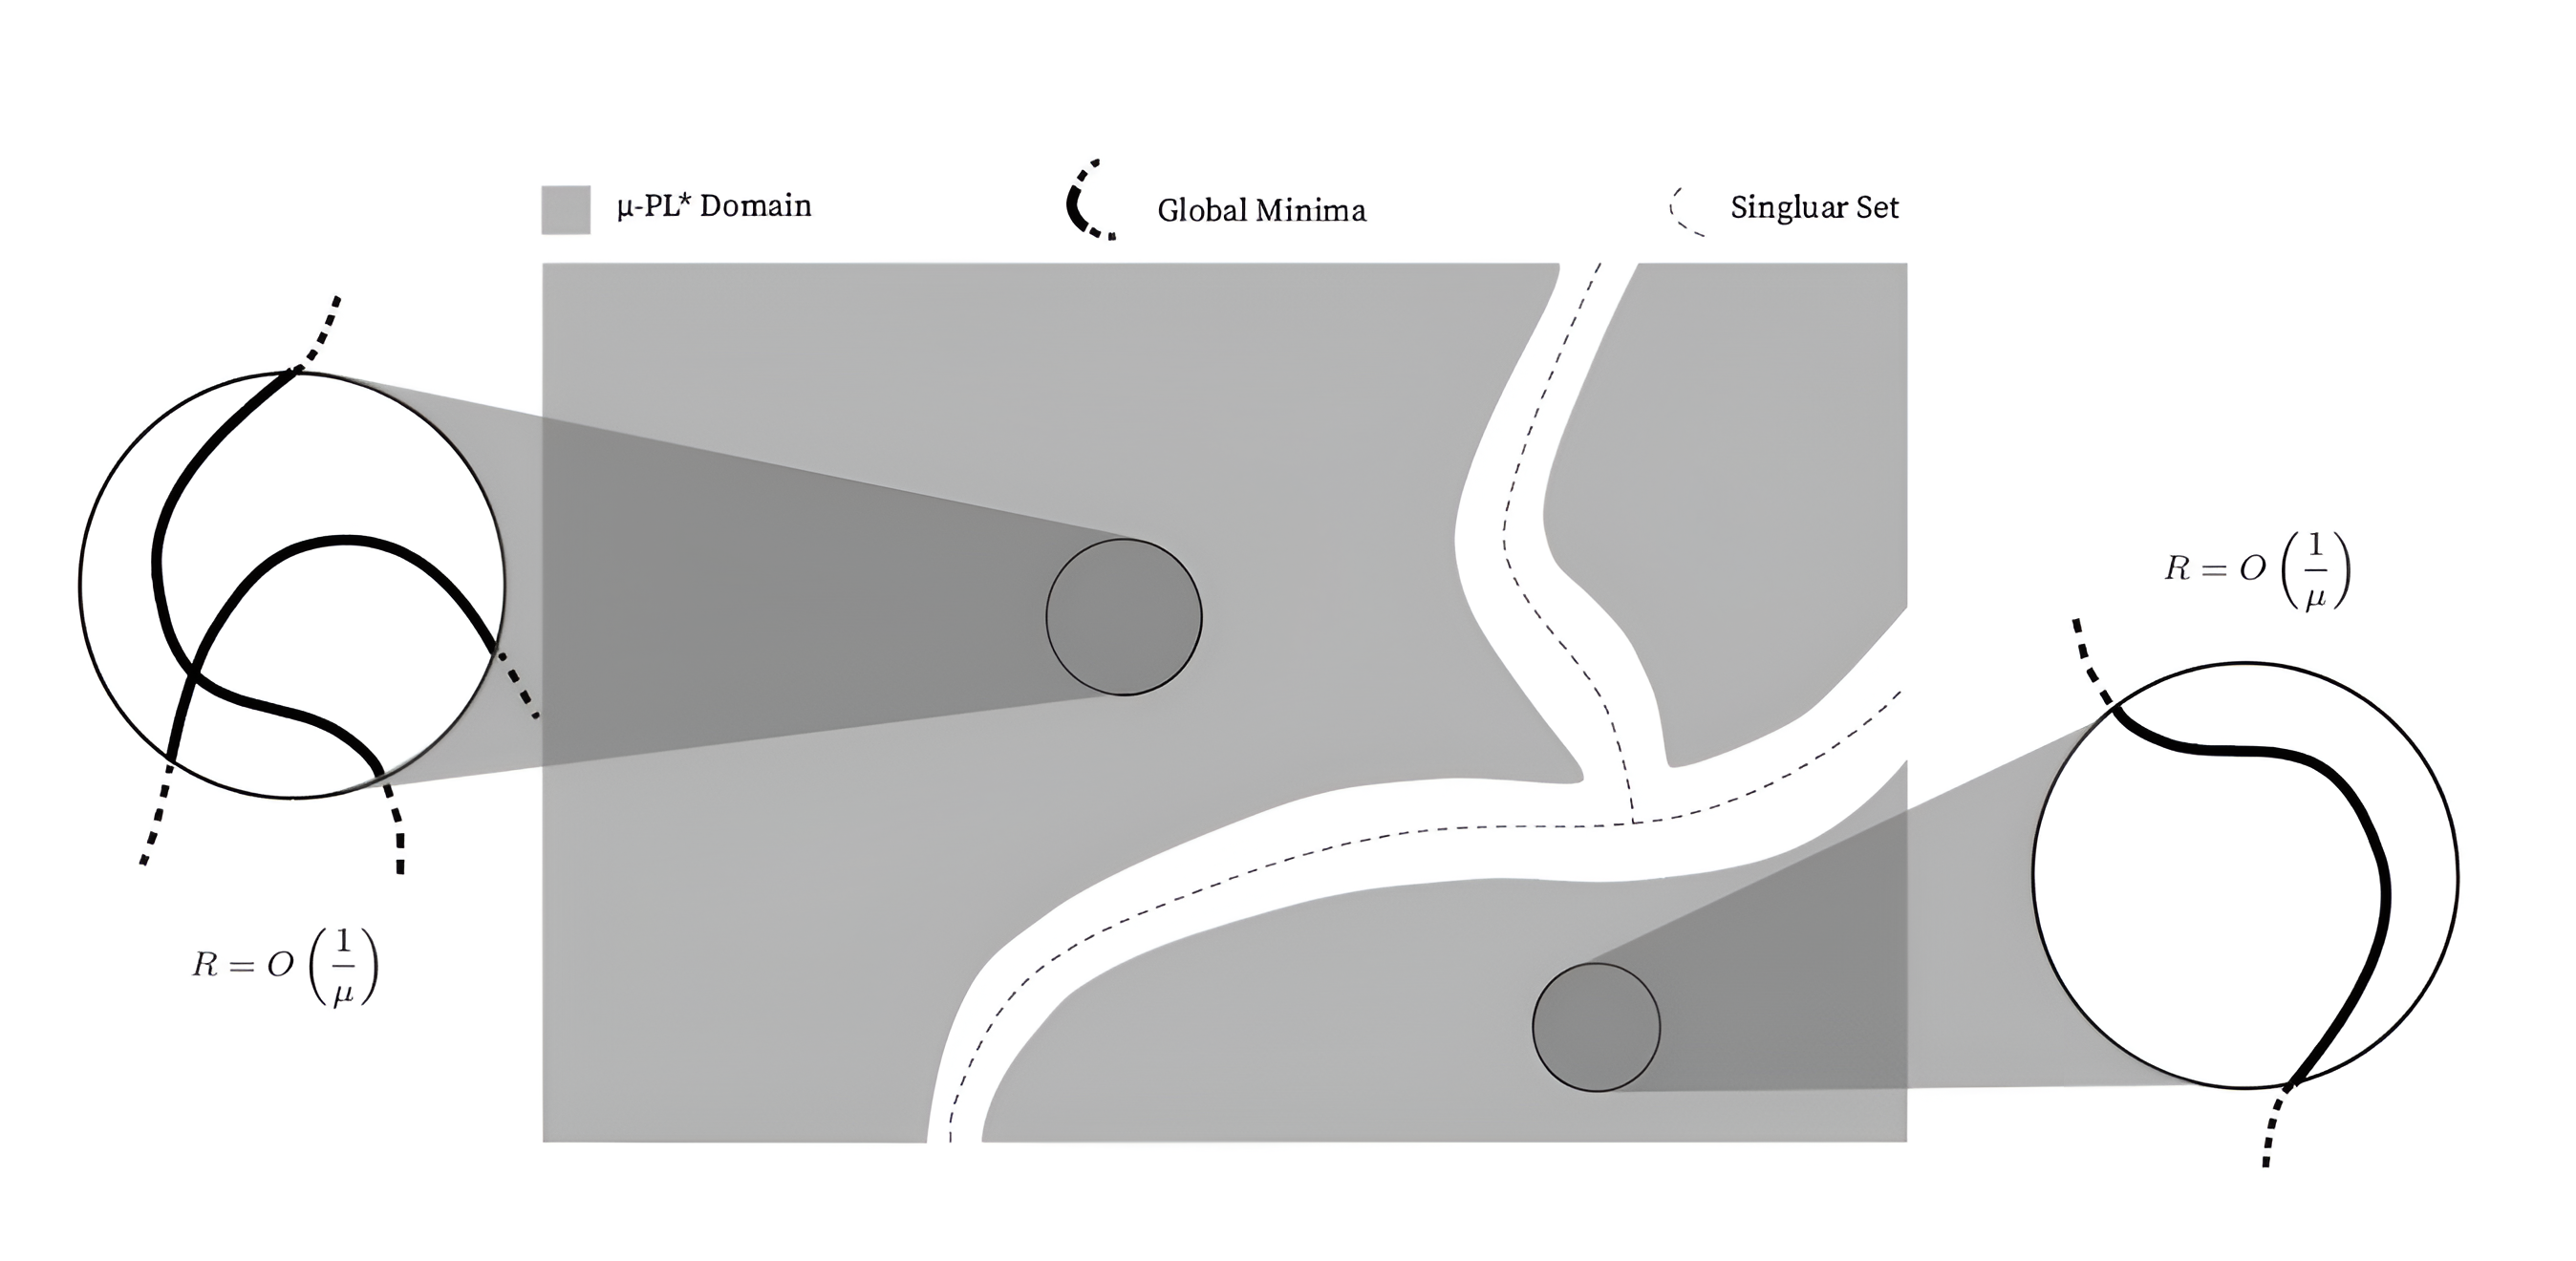
\includegraphics[width=0.8\linewidth]{img/cosarara2.png}
    \caption[Ejemplo de función de pérdida que satisface la condición $\mu$-PL~\cite{Liu2021}.]{Ejemplo de función de pérdida que satisface la condición $\mu$-PL~\cite{Liu2021}. La función de pérdida es $\mu$-PL en la zona sombreada. El conjunto singular corresponde a los vectores $w$ con núcleo tangente degenerado. Cada bola de radio $R = O\left(\frac{1}{\mu}\right)$ dentro del dominio $\mu$-PL se interseca con el conjunto de mínimos globales de la función de pérdida.}\label{fig:cosarara2}
\end{figure}

Aplicando un razonamiento similar, cuando $P > N$, esperamos que $\mathcal{S}_{\text{sing}}$ tenga codimensión positiva ($P - N + 1$) y sea un conjunto de medida cero. Esto significa que, dentro de un conjunto compacto, para valores suficientemente pequeños de $\mu$, es probable encontrar puntos que no satisfacen la condición $\mu$-PL alrededor de $\mathcal{S}_{\text{sing}}$, el cual es un subconjunto de baja dimensión en $\mathbb{R}^P$. Esto puede observarse en la Figura~\ref{fig:cosarara2}. Es importante notar que, cuanto mayor sea el grado de sobreparametrización del sistema, mayor será la codimensión esperada del conjunto singular. En otras palabras, la región donde la condición $\mu$-PL no se cumple se vuelve más pequeña en comparación con el espacio total de parámetros.

En contraste, cuando $P < N$, el núcleo tangente es siempre degenerado ($\lambda_{\min}(K(w)) \equiv 0$), por lo que tales sistemas no pueden estar uniformemente condicionados y no pueden satisfacer la condición $\mu$-PL.

\subsection{El impacto del sesgo inductivo en la selección de hipótesis}\label{subsec:suavidad-funcional}

Si bien los resultados presentados anteriormente aseguran la existencia y convergencia, en la zona sobreparametrizada, hacia un minimizador global de la función de pérdida, sabemos que en dicho régimen existe una multitud de minimizadores globales.  

A pesar de que todavía no existe una propuesta concluyente para seleccionar, de entre todas las hipótesis de $S$, aquella que mejor generaliza, se sabe que, aunque todas sean minimizadoras globales (es decir, satisfacen $\mathcal{L}(w) = 0$), no necesariamente todas garantizan una buena generalización. Un ejemplo claro de esto se puede observar para el caso de regresores polinómicos en la Figura~\ref{fig:suavidad1}, donde, una vez que tenemos suficientes parámetros para ajustar todos los datos de entrenamiento, empezamos a obtener distintos modelos que son minimizadores globales.

\begin{figure}[h!]
    \centering
    \begin{minipage}{0.45\textwidth}
        \centering
        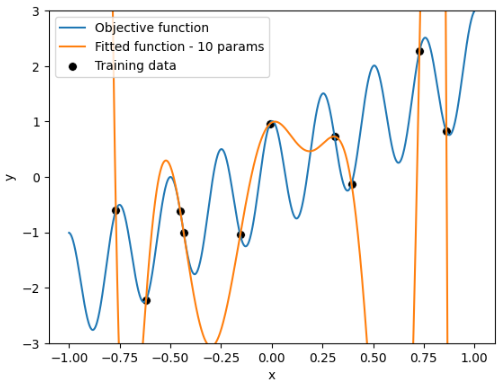
\includegraphics[width=\linewidth]{img/experiments/legendre1.2.png}
    \end{minipage}
    \hfill
    \begin{minipage}{0.45\textwidth}
        \centering
        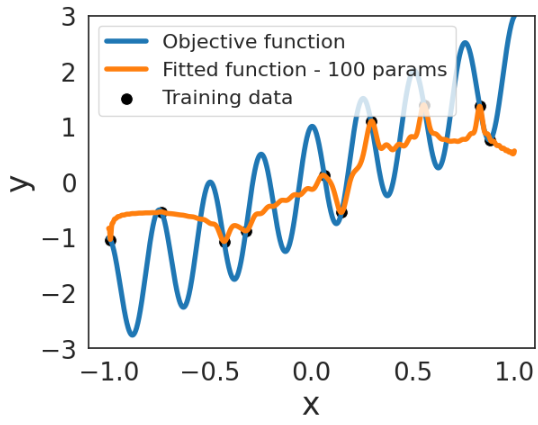
\includegraphics[width=\linewidth]{img/experiments/legendre1.3.png}
    \end{minipage}
    \caption[Distintos modelos polinómicos para aproximar una función.]{Distintos modelos polinómicos (línea naranja) para aproximar una función objetivo (línea azul). Ambos modelos se ajustan de manera perfecta a los datos de entrenamiento (puntos azules). Sin embargo, el modelo de la derecha generaliza mejor al estar regularizado y suavizado hacia una solución de norma pequeña. Imagen del autor inspirada en~\cite{Schaeffer2023}.}\label{fig:suavidad1}
\end{figure}

Extrayendo conclusiones de la Figura~\ref{fig:suavidad1} y apoyándonos en la intuición ampliamente compartida dentro de la comunidad científica, se puede postular que una noción adecuada de \textbf{suavidad funcional} podría desempeñar un papel fundamental en la selección del mejor modelo con miras a la generalización.  

La idea de maximizar la suavidad de una función sujeta a la interpolación de los datos representa una forma de actuar según el principio de la navaja de Ockham~\cite{Blumer1987}. Este principio establece que se debe preferir la explicación más simple que sea consistente con las evidencias. En nuestro caso, podemos utilizar como analogía que los datos de entrenamiento representan las evidencias, mientras que la simplicidad se asocia con la ``suavidad'' de la hipótesis a elegir. De esta manera, el principio de la máxima suavidad se puede formular como: ``\textit{Elegir la función más suave, de acuerdo con alguna noción de suavidad funcional, entre todas las que son minimizadoras globales}''~\cite{Belkin2021}.

Este comportamiento también se encuentra asociado, en cierta medida, al conjunto de hipótesis $\mathcal{H}$ del modelo. Si consideramos dos conjuntos de hipótesis $\mathcal{H}_1$ y $\mathcal{H}_2$, de manera que $\mathcal{H}_1 \subset \mathcal{H}_2$, y sus correspondientes subconjuntos que contienen las hipótesis que son minimizadoras globales, $S_1 \subset \mathcal{H}_1$ y $S_2 \subset \mathcal{H}_2$, entonces, estos conjuntos estan relacionados por la misma inclusión ($S_1 \subset S_2$).

Por tanto, si $\| \cdot \|_{s}$ es cualquier norma funcional, o más generalmente, cualquier funcional, se verifica que

\[
    \min_{g \in S_2} \| g \|_{s} \leq \min_{g \in S_1} \| g \|_{s}.
\]

Suponiendo que $\| \cdot \|_{s}$ es el sesgo inductivo correcto, que mide esa suavidad (por ejemplo, una norma de Sobolev), entonces esperamos que la hipótesis elegida de $S_2$ sea más suave, debido a que este conjunto contiene un mayor número de hipótesis que el conjunto $S_1$ y, por tanto, este conjunto es más adecuado para resolver el problema, lo que lleva a una mejor generalización de la hipótesis elegida.

El principio enunciado anteriormente también permite explicar la aparición del máximo en el error de generalización cerca del umbral de interpolación, ya que en ese punto el modelo se ve forzado a pasar exactamente por cada uno de los puntos de entrenamiento. Esto conduce a una solución única que depende exclusivamente de los datos de entrenamiento, lo que obliga al modelo a seleccionar dicha solución independientemente de su ``suavidad''.

Ligado a esto, Somepalli et al.~\cite{Somepalli2022} analizaron la reproducibilidad de los resultados obtenidos por las mismas redes neuronales a partir del estudio de sus fronteras de decisión. Para nuestro interés, observaron que cerca del umbral de interpolación, y de forma más notable en presencia de ruido, las regiones de decisión tienden a fragmentarse en áreas más pequeñas, las cuales, por lo general, no son reproducibles entre diferentes ejecuciones. En contraste, fuera de este umbral, hay un menor número de regiones de decisión y se encuentran bien definidas, siendo en cierta medida más ``suaves'' (véase Figura~\ref{fig:ground-truth-reproducibility}).

\begin{figure}[h]
    \centering
    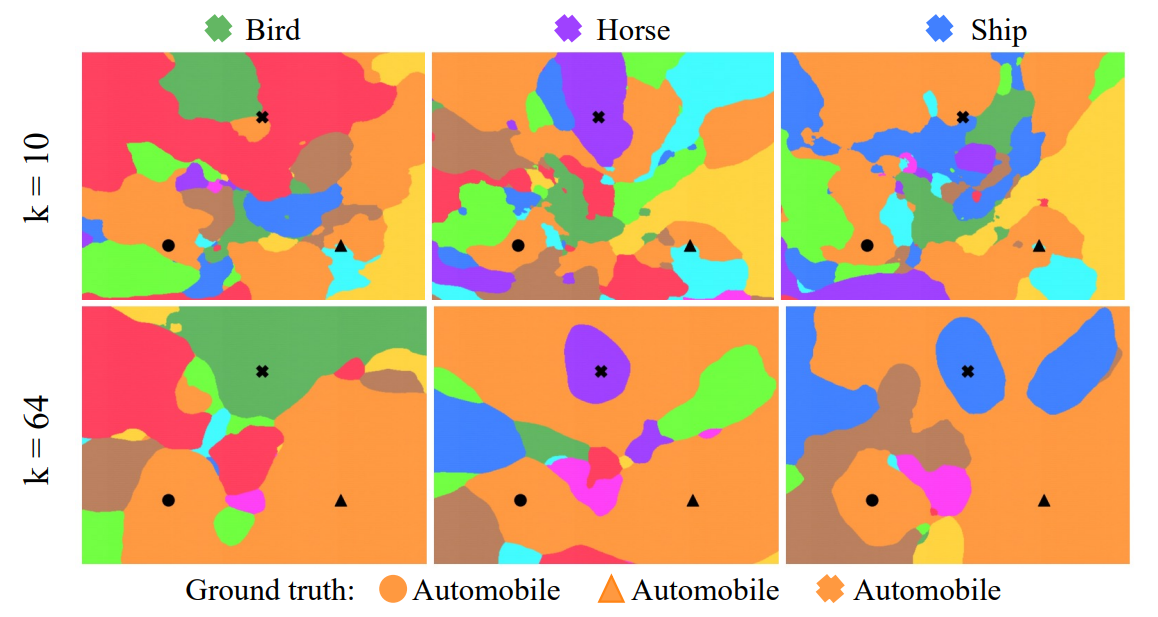
\includegraphics[width=0.6\linewidth]{img/ground-truth-reproducibility.png}
    \caption[Fronteras de decisión para modelos con distinta capacidad~\cite{Somepalli2022}.]{Fronteras de decisión para modelos con distinta capacidad~\cite{Somepalli2022}. Cada columna representa una tripleta distinta de imágenes, en la que una imagen de automóvil (marcada con una $\times$) ha sido etiquetada incorrectamente. El modelo infraparametrizado ($k=10$) genera numerosas regiones de decisión pequeñas y fragmentadas, mientras que el modelo sobreparametrizado ($k=64$) produce un menor número de regiones, más amplias y claramente definidas.}\label{fig:ground-truth-reproducibility}
\end{figure}

Finalmente, a partir de una puntuación de reproducibilidad basada en dichas regiones de decisión, observaron que esta métrica toma valores más bajos cerca del umbral de interpolación. Esto sugiere que, en dicha región, el modelo seleccionado tiende a ser más particular y depende fuertemente de la inicialización de los parámetros de la red utilizada.

Generalmente, puede pensarse que los sesgos inductivos introducidos por los algoritmos de optimización son de naturaleza restrictiva, es decir, imponen restricciones al espacio de hipótesis que están alineadas con el problema de interés. En otras palabras, dado que existen múltiples configuraciones del modelo que se ajustan adecuadamente a los datos pero generan una mala generalización, se prefiere restringir el espacio de hipótesis a aquellas configuraciones que tienden a generalizar mejor para el problema en cuestión, independientemente de si estas son óptimas en un sentido más amplio. Este enfoque está estrechamente relacionado con los principios de regularización.

Al reducir el espacio de hipótesis, este se ve más rápidamente limitado por los datos, ya que existen menos opciones para que el modelo se ajuste a ellos. No obstante, estos sesgos restrictivos pueden considerarse, en ciertos contextos, como indeseables. En efecto, lo que se busca es respaldar cualquier solución capaz de describir adecuadamente los datos, lo que implica favorecer un espacio de hipótesis lo suficientemente flexible.

\begin{figure}[h]
    \centering
    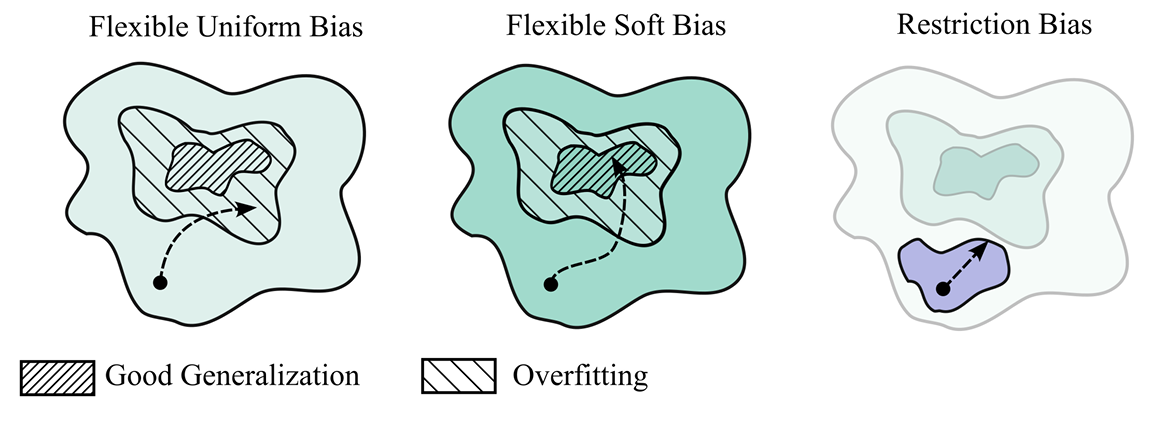
\includegraphics[width=0.6\linewidth]{img/types-of-bias.png}
    \caption[Diferentes tipos de sesgo para el espacio de hipótesis~\cite{Wilson2025}.]{Diferentes tipos de sesgo para el espacio de hipótesis~\cite{Wilson2025}. A la izquierda observamos un conjunto de hipótesis grande sobre el cual no se tiene preferencia por las soluciones que ajustan igualmente bien los datos. En este caso, el entrenamiento puede derivar en soluciones de sobreajuste que generalizan mal. En el centro, se presenta un conjunto de hipótesis flexible en combinación con un sesgo inductivo suave, que guía el entrenamiento hacia soluciones que generalizan bien. A la derecha, restringir el espacio de hipótesis puede ayudar a evitar el sobreajuste al considerar solo algunas soluciones. Sin embargo, al limitar la expresividad del modelo, se impide captar todos los matices de la realidad, lo que dificulta alcanzar la mejor generalización.}\label{fig:types-of-bias}
\end{figure}

La idea general de preferir ciertas soluciones sobre otras, incluso cuando ambas se ajustan igualmente a los datos, se conoce como \textbf{sesgo inductivo suave}~\cite{Wilson2025}. La Figura~\ref{fig:types-of-bias} ilustra este concepto, distinguiéndolo de otros tipos de sesgo. El hecho de considerar estos sesgos inductivos suaves se relaciona directamente con la disminución de la varianza (y, por lo tanto, también del error) a medida que aumentamos la capacidad del modelo. Este tipo de sesgos se centra en una zona específica (y favorable) del espacio de hipótesis, reduciendo así la varianza asociada. Es comparable a utilizar un sesgo restrictivo, pero enfocado en un subconjunto adecuado de hipótesis, como puede observarse en la Figura~\ref{fig:types-of-bias}.

Por otro lado, a medida que aumenta la cantidad de parámetros, también crece el volumen de soluciones planas en el paisaje de la función de pérdida (como se ha observado en la subsección anterior), lo que facilita el acceso y la selección de una de ellas~\cite{Huang2020}. Así, los modelos más grandes (sobreparametrizados) presentan sesgos inductivos más pronunciados, como se puede observar en la Figura~\ref{fig:overparametrization}.

\begin{figure}[h]
    \centering
    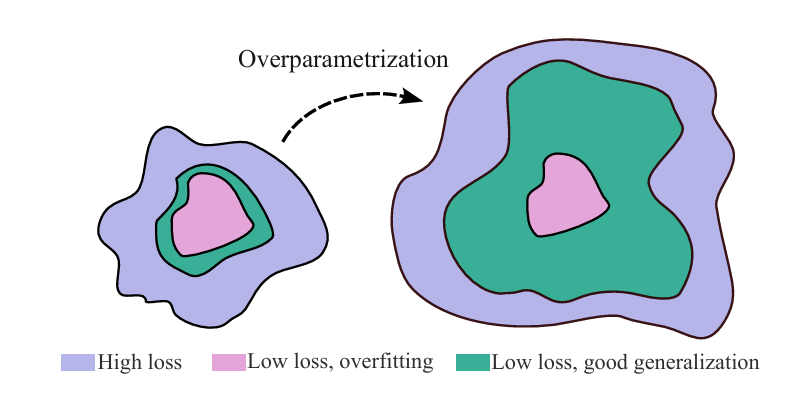
\includegraphics[width=0.5\linewidth]{img/overparametrization.png}
    \caption[Aumentar la capacidad de un modelo mejora su generalización~\cite{Wilson2025}.]{Aumentar la capacidad de un modelo mejora su generalización~\cite{Wilson2025}. Al aumentar el número de parámetros de un modelo, las soluciones ``planas'' ocupan un mayor volumen dentro del espacio total de hipótesis, lo que implica un sesgo inductivo suave hacia ellas. Aunque los modelos sobreparametrizados presentan muchas hipótesis que sobreajustan los datos, también pueden contener muchas otras que se ajustan bien a los datos y proporcionan una buena generalización. De este modo, la sobreparametrización puede aumentar simultáneamente el tamaño del espacio de hipótesis y del sesgo hacia soluciones más simples.}\label{fig:overparametrization}
\end{figure}

Ligado a la explicación del fenómeno de la generalización, también surge el siguiente resultado~\cite{Maddox2020}, ampliamente relacionado con lo presentado en la Subsección~\ref{subsec:analisis-intuitivo-minimos-cuadrados}.

\begin{definicion}(Dimensionalidad efectiva)
    Sea $A \in \mathcal{M}_{n \times n}(\mathbb{R})$ una matriz simétrica. Se define su dimensionalidad efectiva como

    \[
        N_{eff}(A) = \sum_{i=1}^{n}\frac{\lambda_i}{\lambda_i + \alpha},
    \]

    donde $\lambda_i$ son los valores propios de la matriz $A$ y $\alpha > 0$ es una constante de regularización.
\end{definicion}

Así, la dimensionalidad efectiva mide el número de valores propios relativamente grandes, lo que puede interpretarse como una medida de las direcciones significativas en el espacio de parámetros. En particular, la dimensionalidad efectiva de la matriz Hessiana de la función de pérdida, evaluada en el vector de parámetros $w$, cuantifica el número de direcciones agudas (direcciones con curvatura) en el paisaje de pérdidas, es decir, el número de parámetros que están determinados por los datos.

Maddox et al.~\cite{Maddox2020} descubrieron que, después del entrenamiento, los modelos grandes tienen menos parámetros efectivos que los modelos más pequeños, al observar su dimensionalidad efectiva. En trabajos más recientes, Goldblum et al.~($2024$)~\cite{Goldblum2024} también demostraron que los LLM presentan un fuerte sesgo hacia soluciones más simples, y que este sesgo es una característica clave para un buen rendimiento. Estos resultados refuerzan la conjetura de que las soluciones más simples tienden a obtener mejores resultados, ya que son más comprensibles y siguen la filosofía de Ockham. Asimismo, el sesgo inductivo hacia estas soluciones contrarresta, de alguna manera, el crecimiento del número de soluciones que no son minimizadoras globales~\cite{Mingard2023}.

Como conlusión, podemos decir que el uso de sistemas sobreparametrizados resulta ventajoso para obtener cada vez más soluciones posibles (minimizadores globales) para nuestro problema. De esta forma, al aumentar la capacidad del modelo (en nuestro caso, su complejidad efectiva), resultará más sencillo para el algoritmo de optimización elegir una ``buena'' hipótesis (que generalice mejor que el resto) basada en algún sesgo inductivo que utilice. Este sesgo parece ir ligado hacia soluciones más simples, donde, en el caso de las hipótesis, se pueden entender como más ``suaves'', lo que conduce a la hipótesis elegida a una especie de autoregulación.

\subsection{PAC-Bayes y límite de hipótesis numerables}\label{subsec:pac-bayes}

Los marcos de generalización clásicos, como la complejidad de Rademacher o la dimensión VC (véase Sección~\ref{sec:marcos-generalizacion-clasicos}), desafían, por tanto, las nuevas nociones y límites de generalización, ya que penalizan el tamaño total del conjunto de hipótesis. Esto sugiere una recomendación hacia sesgos restrictivos, en lugar de promover sesgos inductivos suaves, como se mencionó anteriormente. Por esta razón, en esta subsección buscamos introducir nuevos marcos que se alineen con las ideas más recientes, presentados en~\cite{Wilson2025}.

Estos nuevos marcos de generalización, aunque no son novedosos y han existido durante décadas, incluyen enfoques como PAC-Bayes~\cite{McAllester1999} y límites de hipótesis numerables~\cite{Valiant1984}. Estos ofrecen un enfoque convincente para modelos sobreparametrizados, ya que se centran en identificar qué hipótesis son probables, en lugar de penalizar el tamaño del espacio de hipótesis. De este modo, siguen la tendencia de los sesgos inductivos suaves.

\begin{teorema}[Límite de hipótesis numerables]
    Sea el riesgo acotado $\mathcal{L}(g) \in [a, a + \Delta]$ y un espacio de hipótesis numerable $\mathcal{H}$ para el cual se dispone de una distribución a priori $P(g)$ de la hipótesis $g$. Sea $\mathcal{L}_{emp}(g)$ el riesgo empírico y $\mathcal{L}(g) = \mathbb{E}[\mathcal{L}_{emp}(g)]$ el riesgo real. Entonces, con probabilidad al menos $1 - \delta$,

    \begin{equation}\label{eq:pac-bayes1}
        \mathcal{L}(g) \leq \mathcal{L}_{emp}(g) + \Delta \sqrt{ \frac{ \log \left( \frac{1}{P(h)} \right) + \log \left( \frac{1}{\delta} \right)}{2n}}.
    \end{equation}
    
\end{teorema}
    
Esta cota está relacionada con la cota para espacios finitos de hipótesis, pero incluye una distribución a priori $P(h)$ que pondera las distintas hipótesis, y un espacio de hipótesis numerable en lugar de finito. Además, podemos usar cualquier distribución a priori para evaluar la cota, sin necesidad de que contenga la hipótesis objetivo.

A partir de la ecuación~\eqref{eq:pac-bayes1}, podemos derivar cotas más informativas utilizando una distribución a priori de Solomonoff $P(g) \leq 2^{-K(g|A)}$~\cite{Solomonoff1964}, donde $K$ es la \textit{complejidad de Kolmogorov libre de prefijo} de $g$ (longitud del programa más corto que produce $g$ utilizando un lenguaje de programación fijo) al tomar como entrada la arquitectura del modelo $A$. Sustituyendo esta cota en la ecuación~\eqref{eq:pac-bayes1}, obtenemos:

\begin{equation}\label{eq:pac-bayes2}
    \mathcal{L}(g) \leq \mathcal{L}_{emp}(g) + \Delta \sqrt{ \frac{ K(g|A)\log (2) + \log \left( \frac{1}{\delta} \right) }{2n} }.
\end{equation}

Aunque en general no podemos calcular el programa más corto, sí podemos acotar la arquitectura y cualquier constante no determinada por los datos dentro de la distribución a priori, utilizando la probabilidad condicionada $K(g|A)$. Esta complejidad puede ser convertida desde la versión libre de prefijo a la complejidad de Kolmogorov estándar, obteniendo la siguiente cota superior:

\begin{equation}
    \log \left( \frac{1}{P(g)} \right) \leq K(g|A)\log (2) \leq C(g)\log (2) + 2\log (C(g)),
\end{equation}
    
donde $C(g)$ es el número de bits requeridos para representar la hipótesis $g$ usando algún código específico predefinido. Por tanto, incluso modelos con mucha capacidad pueden tener garantías sólidas de generalización a través de la ecuación~\eqref{eq:pac-bayes2}.

Las cotas PAC-Bayes permiten reducir la cantidad de bits desde $\log_2 \left( \frac{1}{P(g)} \right)$ hasta la divergencia de Kullback-Leibler $\text{KL}(Q \| P)$, al considerar una distribución de soluciones deseables $Q$. Estos marcos de generalización han sido adaptados para ofrecer garantías de generalización no triviales en modelos con millones de parámetros, incluyendo redes neuronales y grandes modelos de lenguaje (LLMs)~\cite{Lotfi2024}.

En resumen, estos marcos sugieren que las cotas de generalización pueden interpretarse de la siguiente forma:

\[
    \text{Riesgo real} \leq \text{Riesgo empírico} + \text{Compresibilidad del modelo},
\]

donde la compresibilidad proporciona una cierta formalización de complejidad.

Este enfoque se relaciona con la inducción de Solomonoff, que propone un procedimiento de aprendizaje ideal y sobreparametrizado al máximo sin límite en la complejidad de la hipótesis~\cite{Solomonoff1964}. Al asignar pesos exponencialmente mayores a programas más simples, la inducción de Solomonoff garantiza que, aunque el espacio de hipótesis sea enorme, la hipótesis elegida será simple si se ajusta bien a los datos.

En conclusión, estas ``nuevas'' cotas de generalización tienden a volverse más estrictas, y no más laxas como ocurre con las cotas clásicas, al utilizar modelos más grandes. Esto se debe a que dichos modelos tienden a seleccionar soluciones más simples, en línea con la noción de sesgos inductivos suaves, como se discutió en secciones anteriores. Además, estos límites pueden ser sorprendentemente precisos~\cite{Lotfi2022}.

\section{Aproximación no lineal}\label{sec:aproximacion-no-lineal}

En esta sección, introduciremos algunos elementos fundamentales de la teoría de la aproximación no lineal~\cite{DeVore1998}, la cual está relacionada con el problema del aprendizaje profundo. Además, desarrollaremos ciertos conceptos con el propósito de demostrar la existencia de analogías entre esta teoría y el fenómeno conocido como \textit{Deep Double Descent}, así como de proporcionar una posible explicación desde esta perspectiva.

Comenzamos recordando que el problema principal de la teoría de la aproximación es encontrar una representación para una función, generalmente compleja, denominada función objetivo $f$, utilizando funciones más simples llamadas \textbf{aproximantes}. De esta manera, al igual que en el caso del aprendizaje, ambos enfoques buscan aproximar una determinada función a partir de otras más sencillas.

La aproximación no lineal implica que los aproximantes no provienen de espacios lineales, sino de variedades no lineales. Dado que el incremento en la resolución de la función objetivo solo puede lograrse aumentando la complejidad de los aproximantes, resulta lógico considerar que la aproximación no lineal ofrece ventajas sobre los métodos clásicos. Para evaluar esto, estudiaremos la tasa de aproximación, definida como la disminución del error en función del número de parámetros en el aproximante, en relación con el doble descenso.

Por tanto, la idea de no restringir las aproximaciones a espacios lineales consiste en utilizar una malla más fina en las regiones donde la función objetivo no es muy suave (presenta singularidades) y una malla más gruesa donde sí lo es. No obstante, será necesario caracterizar formalmente esta noción de suavidad para obtener resultados concluyentes.

Finalmente, nos centraremos en la aproximación no lineal conocida como aproximación de $n$ términos, que consiste en mantener el control únicamente sobre el número de términos a utilizar para realizar la aproximación, dejando que la selección de los términos dependa de la función objetivo. Esto conduce a un problema de doble etapa, en el que la función objetivo se utiliza tanto para seleccionar una base adecuada de una biblioteca de bases como para elegir la mejor aproximación de $n$ términos en relación con dicha base.

\subsection{Aproximación en un espacio de Hilbert}

Dado que los problemas de la teoría de la aproximación son más sencillos de analizar en un espacio de Hilbert, comenzaremos con una breve discusión sobre este entorno, con el fin de introducir los conceptos clave.

Por ello, sea $\mathcal{H}$ un espacio de Hilbert con producto interno $\langle \cdot, \cdot \rangle$ y norma $\|\cdot\|_{\mathcal{H}}$, y sea $\{\eta_k\}_{k=1}^{n}$ una base ortonormal de $\mathcal{H}$. De esta manera, en el caso en el que el espacio $\mathcal{H}$ tenga dimensión infinita, la base ortonormal también será infinita. Para el caso de la aproximación lineal, consideramos el espacio lineal $\mathcal{H}_n = \text{span}\{\eta_k : 1 \leq k \leq n\}$ para aproximar un elemento $f \in \mathcal{H}$. El error de aproximación se mide mediante
\[
    E_n(f)_{\mathcal{H}} = \inf_{g \in \mathcal{H}_n} \| f - g \|_{\mathcal{H}}.
\]

Como contraparte en la aproximación no lineal, que es el caso de estudio de este análisis, contamos con la aproximación de $n$ términos, que reemplaza $\mathcal{H}_n$ por el espacio $\Sigma_n$, el cual consiste en todos los elementos $g \in \mathcal{H}$ que pueden expresarse como
\[
    g = \sum_{k \in \Lambda} c_k \eta_k,
\]
donde $\Lambda \subset \mathbb{N}$ es un conjunto de índices con $\# \Lambda \leq n$ (cardinalidad finita).

Es claro que, a diferencia de $\mathcal{H}_n$, el espacio $\Sigma_n$ no es lineal. De manera análoga al error de aproximación lineal $E_n$, definimos el error de aproximación de $n$ términos como

\[
    \sigma_n(f)_{\mathcal{H}} = \inf_{g \in \Sigma_n} \| f - g \|_{\mathcal{H}}.
\]

\begin{definicion}
    Dado un número real $\alpha > 0$, denotamos por $\mathcal{A}^{\alpha}(\Sigma_n)$ la clase de funciones $f \in \mathcal{H}$ que cumplen la siguiente desigualdad para algún $M > 0$:

    \begin{equation}\label{eq:clases-error}
        \sigma_n(f)_{\mathcal{H}} \leq M n^{-\alpha}, \quad n \in \mathbb{N}.
    \end{equation}

    Además, definimos la seminorma $|f|_{\mathcal{A}^{\alpha}(\Sigma_n)}$ como el ínfimo de todos los valores de $M$ para los cuales se cumple la ecuación anterior.
\end{definicion}

Denominaremos al conjunto $\mathcal{A}^{\alpha}$ como un \textbf{espacio de aproximación}, el cual agrupa las funciones $f \in \mathcal{H}$ con un comportamiento de aproximación similar, es decir, aquellas cuyo error de aproximación disminuye con una tasa de orden $n^{-\alpha}$.

Finalmente, podemos caracterizar el espacio $\mathcal{A}^{\alpha}(\Sigma_n)$ como una serie en términos de la base ortonormal de $\mathcal{H}$, reorganizando dicha base para que los coeficientes de la función $f$ sean decrecientes. Por tanto, denotamos $f = \sum_{k=1}^{\infty} \gamma_k(f) \eta_k$ una vez reordenada la base de modo decreciente en los coeficientes $\gamma_k(f)$. De esta manera, representamos por $\gamma_k(f)$ al valor absoluto del $k$-ésimo coeficiente de la función $f$. 

\begin{teorema}
    Una función $f \in \mathcal{A}^{\alpha}(\Sigma_n)$ si y solo si se cumple la siguiente desigualdad:

    \begin{equation}\label{eq:coeficientes-reordenados1}
        \gamma_n(f) \leq M n^{-\alpha - 1/2},
    \end{equation}

    donde el ínfimo de todos los $M$ que satisfacen la ecuación anterior es equivalente a la seminorma $|f|_{\mathcal{A}^{\alpha}(\Sigma_n)}$.
\end{teorema}

\begin{proof}
    En primer lugar, notemos que

    \[
        \sigma_n(f)^2_{\mathcal{H}} = \sum_{k>n} \gamma_k(f)^2,
    \]

    dado que el error de aproximación al cuadrado es la suma de los cuadrados de los coeficientes que no están involucrados en la aproximación. Por tanto, si $f$ cumple la hipótesis~\eqref{eq:coeficientes-reordenados1}, entonces

    \begin{equation}\label{eq:Aalpha1}
        \sum_{k>n} \gamma_k(f)^2 \leq M^2 \sum_{k>n} k^{-2\alpha - 1} = M^2 \sum_{k>n} \frac{1}{k^{2\alpha + 1}}.
    \end{equation}

    Es decir, $\sum_{k>n} \frac{1}{k^{2\alpha + 1}}$ es una serie armónica convergente, ya que $\alpha > 0$. De esta manera, se puede acotar la ecuación~\eqref{eq:Aalpha1} por

    \[
        M^2 \sum_{k>n} \frac{1}{k^{2\alpha + 1}} \leq M^2 \int_{n}^{\infty} \frac{1}{x^{2\alpha + 1}}dx = \frac{M^2}{2\alpha}n^{-2\alpha}.
    \]

    En consecuencia,

    \[
        \sigma_n(f)^2_{\mathcal{H}} \leq \frac{M^2}{2\alpha}n^{-2\alpha} \implies \sigma_n(f)_{\mathcal{H}} \leq \frac{M}{\sqrt{2\alpha}}n^{\alpha} = C M n^{-\alpha},
    \]

    con $C = \frac{1}{\sqrt{2\alpha}}$, lo que demuestra que $f \in \mathcal{A}^{\alpha}(\Sigma_n)$. Por otro lado, si $f \in \mathcal{A}^{\alpha}(\Sigma_n)$, entonces se satisface la siguiente desigualdad:

    \[
        \gamma_{2n}(f)^2 \leq n^{-1} \sum_{m=n+1}^{2n} \gamma_m(f)^2 \leq n^{-1} \sigma_n(f)_{\mathcal{H}}^2 \leq |f|_{\mathcal{A}^{\alpha}(\Sigma_n)}^2 n^{-2\alpha - 1} \leq M^2 n^{-2\alpha - 1}.
    \]

    Una desigualdad análoga se verifica para los coeficientes impares $\gamma_{2n+1}(f)$, debido a la naturaleza decreciente de los mismos. De esta forma, la suma de los cuadrados de los coeficientes (ya sean pares o impares) está acotada de manera similar. Finalmente, aplicando raíces a los resultados obtenidos se obtiene la implicación restante.
\end{proof}

A su vez, definimos el espacio de aproximación $\mathcal{A}_{\infty}^{\alpha}(\Sigma_n)$ como el conjunto de todas las funciones $f \in \mathcal{H}$ tales que

\[
    \sup_{n \geq 1} n^{\alpha} \sigma_n(f)_{\mathcal{H}} < \infty.
\]

Es decir, este conjunto está compuesto por todas las funciones $f \in \mathcal{H}$ que cumplen que

\[
    \sigma_n(f)_{\mathcal{H}} = O(n^{-\alpha}), \quad n \to \infty.
\]

Esto significa que, para las funciones $f$ en $\mathcal{A}_{\infty}^{\alpha}(\Sigma_n)$, la sucesión de los errores de aproximación $\sigma_n(f)_{\mathcal{H}}$ decrece de manera suficientemente rápida conforme $n$ crece.

Al mismo tiempo, denotamos por $\ell_{p,q}$ los espacios de sucesiones de Lorentz\footnote{Los espacios de Lorentz son generalizaciones de los espacios $L^{p}$, en el sentido de que $\ell_{p, p} = L^{p}$, y permiten una caracterización más precisa del comportamiento asintótico de las sucesiones. En particular, los espacios $\ell_{p,\infty}$ corresponden a la versión débil de los espacios $L^{p}$.}. Para nuestro desarrollo, nos centraremos únicamente en el espacio $\ell_{p,\infty}$ (el espacio débil $\ell_{p}$), que está formado por todas las sucesiones que satisfacen

\[
    x^{*}(n) \leq M n^{-1/p},
\]

donde $x^{*}(n)$ es el reordenamiento decreciente de la sucesión $|x(n)|$.

Finalmente, el siguiente resultado nos ayuda a relacionar el espacio de aproximación $\mathcal{A}_{\infty}^{\alpha}$ con el espacio débil $\ell_p$ ($\ell_{p,\infty}$).

\begin{teorema}\label{teo:espaciosapprox-espacioslorentz}
    Para una aproximación de $n$ términos en un espacio de Hilbert $\mathcal{H}$, una función $f \in \mathcal{A}_{\infty}^{\alpha}$ si y solo si sus coeficientes $\{ f_k : k \in \mathbb{N}\}$ están en el espacio débil $\ell_{\tau}$ (es decir, en $\ell_{\tau, \infty}$) con $\tau = (\alpha + 1/2)^{-1}$. Además, en este caso, se verifica

    \[
        C_1 |f|_{\mathcal{A}_{\infty}^{\alpha}(\mathcal{H})} \leq \| (f_k) \|_{\ell_{\tau, \infty}} \leq C_2 |f|_{\mathcal{A}_{\infty}^{\alpha}(\mathcal{H})},
    \]

    donde $C_1, C_2 > 0$ son constantes.
\end{teorema}

\subsection{Aproximación altamente no lineal}

Nos preguntamos ahora cómo depende la efectividad de la aproximación de $n$ términos de la base elegida y si se puede conseguir alguna ventaja eligiendo de manera progresiva una base que dependa de la función objetivo. Para ello, llamamos \textbf{biblioteca} a una clase $\mathcal{L}$ de bases. Por simplicidad, centraremos nuestra discusión en aproximaciones en un espacio de Hilbert $\mathcal{H}$ y en bibliotecas de bases ortonormales para $\mathcal{H}$.

Por consiguiente, nuestro problema de aproximación consiste, dada una función objetivo $f \in \mathcal{H}$, en elegir una base $B \in \mathcal{L}$ y una aproximación de $n$ términos a $f$ usando esta base. Llamamos a este tipo de problema de aproximación altamente no lineal, ya que implica una capa adicional de no linealidad en la selección de bases.

No obstante, otra forma de aproximación estrechamente relacionada es la aproximación utilizando $n$ términos desde un \textbf{diccionario} $\mathbb{D} \subset \mathcal{H}$ de funciones, que será nuestro principal objeto de estudio. En nuestro caso, un diccionario se define como un subconjunto arbitrario de $\mathcal{H}$.

Por ejemplo, en el caso de redes neuronales, un diccionario de funciones podría tener la siguiente forma:

\[
    \{ \sigma(w \cdot x + b) : w \in \mathbb{R}^{P}, b \in \mathbb{R} \},
\]

donde $\sigma$ es una función de activación de una variable fija, $w$ es el vector de parámetros y $b$ es el término de sesgo. De esta manera, se aproximan funciones de $P$ variables mediante combinaciones lineales de funciones de dicho conjunto. Generalmente, se requiere que $\sigma$ cumpla con algunas propiedades adicionales (véase Subsección~\ref{subsubsec:capa-de-activacion}).

Otro ejemplo particular de diccionario es utilizar una base ortonormal $B$ para $\mathcal{H}$ y definir el diccionario asociado como sigue:

\[
    \mathbb{D} = \{\pm b : b \in B\},
\]

donde diremos que $\mathbb{D}$ es el diccionario generado por la base $B$.

La característica común de todos los diccionarios es que la familia de funciones utilizada para el proceso de aproximación es \textbf{redundante}. Es decir, hay muchas más funciones en el diccionario de las necesarias para aproximar cualquier función objetivo $f \in \mathcal{H}$. Por tanto, buscamos que esta redundancia incremente la eficiencia de la aproximación, aunque, por otro lado, también podría ralentizar el proceso de búsqueda de buenas aproximaciones.

\subsubsection{Selección óptima de bases}\label{subsubsec:seleccion-optima-bases}

En esta subsección trataremos cómo la selección adecuada de una base influye directamente en el error de aproximación. Asimismo, observaremos que, al disponer de una biblioteca de bases, el error de aproximación se minimiza para cualquier aproximación realizada, ya que se consideran todas las bases disponibles.

Sea $B = \{ \eta_k \}$ una base ortonormal para $\mathcal{H}$ y sea $\Sigma_n(B)$ el conjunto de funciones en $\mathcal{H}$ que pueden escribirse como una combinación lineal de $n$ de las funciones $\eta_k$, con $k \in \mathbb{N}$. Además, definimos

\[
    \sigma_n(f, B) = \sigma_n(f,B)_{\mathcal{H}} = \inf_{S \in \Sigma_n(B)} \| f - S \|_{\mathcal{H}}
\]

como el error de aproximación correspondiente respecto a la base $B$.

Recordemos que la disminución de los errores de aproximación $\sigma_n(f, B)$ está completamente determinada por los coeficientes reorganizados de la función $f$. Como antes, sea $\gamma_k(f, B)$ el $k$-ésimo mayor valor absoluto de estos coeficientes. Aplicando el Teorema~\ref{teo:espaciosapprox-espacioslorentz} a los coeficientes $\gamma_n(f, B)$, sabemos que $f \in \mathcal{H}$ está en $\mathcal{A}_\infty^\alpha (\mathcal{H}, B)$, si y solo si $(\gamma_n(f, B))$ está en $\ell_{\tau}$ con $\tau = (\alpha + 1/2)^{-1}$. Además, 

\begin{equation}\label{eq:bases}
    C_1 |f|_{\mathcal{A}_\infty^\alpha} \leq \| \gamma_n(f, B) \|_{\ell_{\tau, \infty}} \leq C_2 |f|_{\mathcal{A}_\infty^\alpha},
\end{equation}

con constantes de equivalencia independientes de la base $B$ elegida.

Supongamos ahora que $\mathcal{L} = \{ B_1, \ldots, B_n \}$ es una biblioteca de bases ortonormales. Definimos el error de aproximación con respecto a $\mathcal{L}$ como sigue

\[
    \sigma_n^{\mathcal{L}}(f)_{\mathcal{H}} = \inf_{B \in \mathcal{L}} \sigma_n(f, B)_{\mathcal{H}}.
\]

A la vista de la ecuación~\eqref{eq:bases}, obtenemos la siguiente cota superior

\begin{equation}\label{eq:bases2}
    \sigma_n^{\mathcal{L}}(f)_{\mathcal{H}} \leq C n^{-\alpha} \inf_{B} \| \gamma_n(f, B) \|_{\ell_r, \infty},
\end{equation}

con $C$ una constante absoluta. Además, para cualquier $\alpha > 0$, se tiene

\begin{equation}\label{eq:bases3}
    \bigcap_{B} \mathcal{A}_\infty^\alpha (\mathcal{H}, B) \subset \mathcal{A}_\infty^\alpha (\mathcal{H}, \mathcal{L}).
\end{equation}

En consecuencia, para cada base ortonormal $B$, la condición $(\gamma_n(f)) \in \ell_{\tau, \infty}$, $\tau = (\alpha + 1/2)^{-1}$, puede verse como una condición de suavidad de la función $f$ relativa a la base $B$. Así, el ínfimo en el lado derecho de la ecuación~\eqref{eq:bases2} puede interpretarse como el ínfimo de condiciones de suavidad relativas a las diferentes bases $B$.

De manera similar, podemos ver las clases $\mathcal{A}_\infty^\alpha (\mathcal{H}, B)$ como clases de suavidad con respecto a la base $B$. De esta forma, una ventaja de la selección óptima de bases es que siempre podemos elegir la base $B \in \mathcal{L}$ en la que $f$ sea más suave.

Por su parte, las ecuaciones~\eqref{eq:bases2} y~\eqref{eq:bases3} muestran que la base más eficiente para aproximar $f$ depende del número de términos utilizados para la aproximación. De esta forma, se pueden construir dos bases, $B_1$ y $B_2$, y una función objetivo $f$ de tal manera que, para ciertos valores de $n$, la elección óptima de base varíe entre $B_1$ y $B_2$. Es decir, para algunos valores de $n$, $B_1$ ofrecerá un mejor error de aproximación, mientras que para otros, $B_2$ es más eficiente, lo que demuestra que no hay una base universalmente mejor para todos los valores de $n$.

\subsubsection{Aproximación usando $n$ términos de un diccionario}\label{subsubsec:approx-n-terms}

Supongamos que $\mathbb{D}$ es un diccionario de funciones en $\mathcal{H}$. Para simplificar, asumimos (sin pérdida de generalidad en la aproximación de $n$ términos) que cada $g \in \mathbb{D}$ tiene norma uno, es decir, $\|g\|_{\mathcal{H}} = 1$, y que $-g \in \mathbb{D}$ siempre que $g \in \mathbb{D}$.

Para cada $n \in \mathbb{N}$, definimos $\Sigma_n := \Sigma_n(\mathbb{D})$ como la colección de todas las funciones en $\mathcal{H}$ que pueden expresarse como una combinación lineal de, como máximo, $n$ elementos de $\mathbb{D}$. Así, cada función $S \in \Sigma_n$ puede escribirse de la forma:

\begin{equation}\label{eq:n-terms1}
    S = \sum_{g \in \Lambda} c_g g, \quad \Lambda \subset \mathbb{D}, \quad \#\Lambda \leq n,
\end{equation}

donde $c_g \in \mathbb{R}$ son los coeficientes. Cabe destacar que un elemento de $\Sigma_n(\mathbb{D})$ puede expresarse de la forma~\eqref{eq:n-terms1} de más de una forma.

\begin{definicion}
    Para una función $f \in \mathcal{H}$, definimos su error de aproximación a partir de un diccionario $\mathbb{D}$ como:

    \[
        \sigma_n(f) := \sigma_n(f, \mathbb{D})_{\mathcal{H}} := \inf_{S \in \Sigma_n} \| f - S \|_{\mathcal{H}}.
    \]
\end{definicion}

Así, nuestro interés se centra en obtener estimaciones para $\sigma_n$ (tanto superiores como inferiores). Para este propósito, introducimos la siguiente forma de medir la suavidad con respecto a un diccionario $\mathbb{D}$.

\begin{definicion}
    Para un diccionario $\mathbb{D}$ y cualquier $\tau > 0$, definimos la clase de funciones:

    \[
        \mathcal{K}_{\tau}^{o}(\mathbb{D}, M) = \left\{ f = \sum_{g \in \Lambda} c_g g : \Lambda \subset \mathbb{D}, \quad \#\Lambda < \infty \quad \text{y} \quad \sum_{g \in \Lambda} |c_g|^{\tau} \leq M^{\tau} \right\},
    \]

    y definimos $\mathcal{K}_{\tau}(\mathbb{D}, M)$ como la clausura en $\mathcal{H}$ de $\mathcal{K}_{\tau}^{o}(\mathbb{D}, M)$. Además, definimos $\mathcal{K}_{\tau}(\mathbb{D})$ como la unión de las clases $\mathcal{K}_{\tau}(\mathbb{D}, M)$ para todo $M > 0$. Para $f \in \mathcal{K}_{\tau}(\mathbb{D})$, definimos la seminorma:

    \[
        |f|_{\mathcal{K}_{\tau}(\mathbb{D})} = \inf\{ M : f \in \mathcal{K}_{\tau}(\mathbb{D}, M) \}.
    \]
\end{definicion}

En otras palabras, $\mathcal{K}_{\tau}^{o}(\mathbb{D}, M)$ está formado por la clase de funciones que se pueden escribir como una combinación lineal de un número finito de elementos de $\mathbb{D}$, de tal manera que la suma de los coeficientes elevados a la potencia $\tau$ se encuentre acotada, controlando así la magnitud de las combinaciones lineales.

Por otro lado, $|f|_{\mathcal{K}_{\tau}(\mathbb{D})}$ nos indica la dificultad de aproximar una función $f$ utilizando una combinación de funciones del diccionario. Cuanto más pequeña sea la seminorma, más sencillo será aproximar la función $f$.

\begin{observacion}
    Cuando $\tau = 1$, $\mathcal{K}_1$ es la clase de funciones que son una combinación convexa de las funciones en $\mathbb{D}$.
\end{observacion}

Para el caso en el que $\mathbb{D}$ es generado por una base $B$ se sigue que la aproximación de $n$ términos desde $\mathbb{D}$ es la misma que la aproximación de $n$ términos desde $B$. En particular, si $\tau = (\alpha + 1/2)^{-1}$ y $B$ es ortonormal, se verifica que:

\begin{equation}\label{eq:n-terms-error}
    \sigma_n(f, \mathbb{D})_{\mathcal{H}} \leq Cn^{-\alpha} |f|_{\mathcal{K}_{\tau}(\mathbb{D})}.
\end{equation}

Sabemos que $Cn^{-\alpha}$ es un factor de decaimiento que describe cómo el error de aproximación disminuye a medida que incrementamos el número de términos $n$ en la aproximación. La constante $C$ es un valor positivo que depende tanto del diccionario como de la función, mientras que la potencia $\alpha$ depende de $\tau$ y de las propiedades de la función objetivo.

De esta forma, la ecuación~\eqref{eq:n-terms-error} nos proporciona una cota superior para el error de aproximación de una función $f$ utilizando una aproximación de $n$ términos, a partir de un diccionario $\mathbb{D}$ generado por una base ortonormal $B$. En consecuencia, el error de aproximación $\sigma_n(f, \mathbb{D})_{\mathcal{H}}$ depende tanto de la suavidad de la función $f$ (medida por $|f|_{\mathcal{K}_{\tau}(\mathbb{D})}$) como del número de términos $n$ empleados en la aproximación.

Finalmente, estamos interesados en verificar si la ecuación~\eqref{eq:n-terms-error} es válida para diccionarios más generales. El siguiente resultado nos proporciona una cota superior para el error de aproximación en estos casos, extendiendo los resultados obtenidos en el caso de diccionarios generados por bases ortonormales.

\begin{teorema}
    Sean $\mathbb{D}$ un diccionario de funciones, $\alpha \geq 1/2$ y $1/\tau = \alpha + 1/2$. Si $f \in K_{\tau}(\mathbb{D})$, entonces

    \begin{equation}\label{eq:n-terms-teo}
        \sigma_m(f, \mathbb{D})_{\mathcal{H}} \leq C |f|_{K_{\tau}(\mathbb{D})} m^{-\alpha} \quad \forall m \in \mathbb{N},
    \end{equation}

    donde $C$ depende de $\tau$.
\end{teorema}

\begin{proof}
    Es suficiente probar la desigualdad~\eqref{eq:n-terms-teo} para funciones $f$ que puedan expresarse como una suma finita $f = \sum_j c_j g_j$, con $g_j \in \mathbb{D}$ y $\sum_j |c_j|^\tau \leq M^\tau$. Sin pérdida de generalidad, podemos suponer que los coeficientes $c_j$ son positivos y están ordenados de manera decreciente.
    
    Definimos la suma parcial de los primeros $n$ términos como $s_1 = \sum_{j=1}^{n} c_j g_j$ y su residuo asociado como $R_1 = f - s_1 = \sum_{j>n} c_j g_j$. Ahora,

    \[
        c_n^\tau \leq \frac{1}{n} \sum_{j=1}^{n} |c_j|^\tau \leq \frac{M^\tau}{n}, \quad n \in \mathbb{N}.
    \]

    Por tanto, tomando la raíz $ \tau $-ésima de ambos lados, y dado que los coeficientes están ordenados de manera decreciente, tenemos que $ c_j \leq M \cdot n^{-1/\tau} $ para $ j > n $, lo que nos lleva a

    \[
        \sum_{j>n} c_j = \sum_{j>n} c_j^{1-\tau} c_j^\tau \leq M^{1-\tau} n^{1-1/\tau} \sum_{j>n} c_j^\tau \leq M n^{1-1/\tau}.
    \]

    Esto implica que $R_1 \in \mathcal{K}_1(\mathbb{D}, M n^{1 - 1/\tau})$. A continuación, se enuncia el Teorema $3.2$ de~\cite{DeVore1996}, el cual utilizaremos para finalizar la demostración.

    \begin{teorema}
        Sea $f \in \mathcal{K}_1(\mathbb{D}, 1)$. Entonces, para el algoritmo Greedy Relajado, se cumple la siguiente estimación:

        \[
            \left\| f - G_{m}^{r}(f) \right\| \leq \frac{2}{\sqrt{m}}, \quad \forall m \geq 1,
        \]

        donde $G_{m}^{r}(f)$ denota la aproximación de $f$ obtenida tras $m$ iteraciones del algoritmo Greedy Relajado.
    \end{teorema}

    Si bien la demostración de este resultado se encuentra fuera de los objetivos de este proyecto, su validez nos permite afirmar que

    \[
        \left\| f - G_{m}^{0}(f) \right\|_{\mathcal{H}} \leq |f|_{\mathcal{K}_1} \cdot m^{-1/2}.
    \]

    A partir de la desigualdad anterior, existe una función $s_2$, que es una combinación lineal de a lo sumo $n$ elementos $g \in \mathbb{D}$, tal que

    \[
        \| f - (s_1 + s_2) \| = \| R_1 - s_2 \| \leq 2M n^{1 - 1/\tau} \cdot n^{-1/2} = 2M n^{-\alpha},
    \]

    de donde se obtiene la desigualdad~\eqref{eq:n-terms-teo}.
\end{proof}

\subsection{Analogía con el \textit{Deep Double Descent}}\label{subsec:analogia-matematica-ddd}

A modo de conclusión de este inciso sobre la teoría de la aproximación no lineal, presentaremos a lo largo de esta sección las similitudes que existen entre dicha teoría y el doble descenso, con el objetivo de establecer ciertas analogías que ofrezcan ideas matemáticas subyacentes asociadas a su ocurrencia.

En primer lugar, el objetivo tanto de la aproximación no lineal como del aprendizaje es esencialmente el mismo: aproximar una función objetivo mediante funciones más simples. En el contexto de la teoría de la aproximación, se suele asumir que se conocen los valores de ciertos funcionales lineales simples aplicados a la función objetivo. En cambio, en el aprendizaje, dicha función es completamente desconocida y solo se tiene acceso a un conjunto finito de observaciones, es decir, se puede interpretar como que se conoce el valor de la aplicación de un número finito de funcionales de evaluación. Asimismo, en ambos contextos se recurre al uso de ``procesos no lineales'' para aproximar la función objetivo, lo que permite capturar comportamientos complejos que no podrían representarse adecuadamente mediante aproximaciones provenientes de espacios lineales.

La base a partir de la cual se construyen los aproximantes también desempeña un papel fundamental. Aunque en el caso de las redes neuronales lo que se utiliza propiamente es un diccionario, este diccionario será dependiente de la base elegida. De esta manera, cuando llevemos a cabo los experimentos relacionados con la aproximación polinómica, veremos cómo la elección de la base influye de manera significativa en los resultados obtenidos, tal como se discutió en la Subsección~\ref{subsubsec:seleccion-optima-bases}. En consecuencia, corroboraremos que ciertas bases resultan más adecuadas para aproximar determinadas funciones. 

De este modo, se puede intuir que los modelos obtienen sus aproximantes a partir de la base elegida hasta alcanzar el umbral de interpolación. Precisamente en ese umbral, el aproximante queda determinado de forma única por el uso completo de la base, lo cual explica que su error de generalización no esté controlado y pueda alcanzar valores elevados.

Por otra parte, al superar el umbral de interpolación, la base pasa a funcionar como un diccionario, es decir, un conjunto redundante de funciones en el que, a medida que aumenta el número de parámetros del modelo, se incorporan nuevas posibilidades de aproximación. Aunque estas funciones adicionales son redundantes, contribuyen a mejorar la capacidad de generalización del modelo, ya que al contar con un mayor número de posibles soluciones, el nuevo conjunto de hipótesis resulta más adecuado para resolver el problema. De hecho, como se observó en la Subsección~\ref{subsubsec:approx-n-terms}, la función objetivo tiende a verse más “suave” a medida que aumenta el diccionario. Finalmente, la elección de una ``buena'' hipótesis de todas las disponibles en el diccionario vendría dada por algún sesgo inductivo del algoritmo de optimización utilizado, tal y como se comentó en la Subsección~\ref{subsec:suavidad-funcional}.

\section{Discusión final}\label{sec:conclusion-matematica}

En esta sección hemos expuesto de forma teórica y detallada el \textit{Deep Double Descent}, unificando el enfoque clásico con la práctica moderna a partir de la noción de complejidad efectiva como medida de complejidad del modelo. A partir de esta definición, se identifican las distintas regiones de comportamiento de un modelo durante el entrenamiento, siendo de especial interés la región sobreparametrizada, en la cual hemos centrado nuestro análisis.

Al mismo tiempo, a partir de la descomposición del error en la suma de sesgo y varianza, se introducen las distintas configuraciones que puede adoptar el error de un modelo. Entre ellas, destaca el fenómeno del doble descenso, el cual surge debido a que el sesgo y la varianza predominan en diferentes regiones del comportamiento del modelo, siendo la varianza la que presenta un comportamiento unimodal. También destacamos que, en la región sobreparametrizada, el conjunto de hipótesis disponibles es mayor. De este modo, el verdadero desafío para comprender el fenómeno reside en entender por qué el algoritmo de aprendizaje selecciona ciertas soluciones dentro de ese conjunto sobre otras, y por qué las hipótesis elegidas tienden a generalizar bien.

A partir de un ejemplo de regresión, se introduce un análisis intuitivo del suceso, en el que se observa que su aparición está estrechamente vinculada al término de la varianza. En particular, se verifica que el máximo del error se produce cerca del umbral de interpolación, debido a la configuración de los valores propios que surgen al resolver el problema de regresión. Ligado a esto, se analiza la convergencia del descenso de gradiente, demostrando que, bajo ciertas hipótesis, dicho algoritmo converge hacia soluciones que son minimizadoras globales en la región sobreparametrizada. Esta propiedad se observa tanto en problemas de regresión como en escenarios con datos separables.

A continuación, se presenta la región sobreparametrizada desde el punto de vista de la optimización. En esta sección, se evidencia la existencia de múltiples soluciones dentro de dicha región, así como la ausencia de convexidad local de la función de pérdida en cualquier vecindad de dichas soluciones. Igualmente, se destaca que, mientras en la zona infraparametrizada las soluciones aparecen de forma aislada, en la zona sobreparametrizada estas conforman variedades continuas. 

Posteriormente, se introduce una propiedad más débil que la convexidad, la cual debe cumplir la función de pérdida para garantizar que el GD converja hacia un mínimo global en la región sobreparametrizada. A pesar de conocer la existencia de múltiples soluciones en la región moderna, es necesario entender por qué el algoritmo de aprendizaje tiende a seleccionar aquellas que generalizan adecuadamente. Para ello, se introduce, de forma informal, un concepto de suavidad funcional que orienta al modelo hacia hipótesis más simples, en línea con la filosofía de Ockham. De este modo, el algoritmo de aprendizaje induce un sesgo inductivo suave que lo lleva a concentrarse en subconjuntos óptimos dentro del espacio de hipótesis, lo que contribuye a reducir la varianza en esta región. En última instancia, se presentan los marcos de generalización aplicables en esta región, los cuales se basan en la preferencia de ciertas hipótesis sobre otras.

Para finalizar esta sección, se introducen conceptos básicos de la teoría de la aproximación no lineal, vinculándolos con el dilema del aprendizaje. A su vez, se presentan ciertas analogías con el doble descenso, mostrando cómo el uso de diccionarios con funciones redundantes permite obtener mejores aproximaciones de la función objetivo. Asimismo, se detallan nociones de suavidad en dichos espacios, reforzando la conexión entre la estructura del modelo y su capacidad de generalización.

Para cerrar este análisis, se presenta la Tabla~\ref{tabla:tabla-conclusion} como resumen de lo que ocurre en las distintas zonas de actuación de un modelo.

\begin{table}[h]
    \centering
    \small 
    \renewcommand{\arraystretch}{0.9} 
    \begin{NiceTabular}{c|c|c|}[color-inside]
        \Block{3-1}{} & \Block[draw, fill={cyan!50}]{3-1}{\textbf{Régimen clásico} \\ \textbf{(infraparametrizado)}} & \Block[draw, fill={cyan!50}]{3-1}{\textbf{Régimen moderno} \\ \textbf{(sobreparametrizado)}} \\ \\ \\

        \hline
        \Block[draw]{3-1}{Conjunto de \\ hipótesis} & \Block[draw]{3-1}{Conjunto subóptimo \\ debido a un sesgo restrictivo} & \Block[draw]{3-1}{Conjunto óptimo \\ debido a un sesgo inductivo suave} \\ \\ \\
        
        \hline
        \Block[draw]{3-1}{Curva de \\ generalización} & \Block[draw]{3-1}{Forma clásica de ``U''} & \Block[draw]{3-1}{Descendiente} \\ \\ \\

        \hline
        \Block[draw]{5-1}{Paisaje de \\ \\ optimización} & \Block[draw]{5-1}{Localmente convexo \\ \\ Mínimos locales aislados} & \Block[draw]{5-1}{No localmente convexo \\ Múltiples mínimos globales formando \\ variedades continuas \\ Cumple la condición $\mu$-PL} \\ \\ \\ \\ \\

        \hline
        \Block[draw]{3-1}{Modelo óptimo} & \Block[draw]{3-1}{\text{Sweet spot} (mínimo de la curva ``U'') \\ (difícil de conseguir)} & \Block[draw]{3-1}{Cualquier minimizador global \\ (fácil de encontrar)} \\ \\ \\

        \hline
        \Block[draw]{3-1}{Convergencia del GD} & \Block[draw]{3-1}{GD converge a un mínimo local} & \Block[draw]{3-1}{GD converge a un mínimo global} \\ \\ \\
        \hline

        \hline
        \Block[draw]{5-1}{Marcos de \\ \\ generalización} & \Block[draw]{5-1}{Dimensión VC \\ \\ Complejidad de Rademacher} & \Block[draw]{5-1}{Límite de hipótesis numerable \\ \\ PAC-Bayes} \\ \\ \\ \\ \\

        \hline
        \Block[draw]{3-1}{Aproximación no lineal} & \Block[draw]{3-1}{Uso de bases (simplicidad/eficiencia) \\ para la aproximación} & \Block[draw]{3-1}{Uso de diccionarios (redundancia) \\ para la aproximación} \\ \\ \\
        \hline


    \end{NiceTabular}
    \caption[Resumen comparativo entre el paradigma clásico y el paradigma moderno.]{Resumen comparativo entre el paradigma clásico y el paradigma moderno.}\label{tabla:tabla-conclusion}
\end{table}

\endinput
% !TeX root = ../tfg.tex
% !TeX encoding = utf8

\chapter{Análisis empírico del Deep Double Descent}\label{ch:analisis-empirico-ddd}

\section{Materiales y métodos}\label{sec:materiales-y-metodos}

\subsection{Datasets}\label{subsec:datasets}

En la parte práctica de este proyecto, se emplearán diversos conjuntos de datos (datasets) etiquetados, pues nos movemos bajo el enfoque del aprendizaje supervisado. Dado que la experimentación se limita a este tipo de aprendizaje, se han seleccionado datasets ampliamente reconocidos y utilizados en problemas de clasificación de imágenes, lo que también nos ayudará a comparar los resultados obtenidos con los de la comunidad científica. A continuación, se detallarán los principales datasets utilizados en este estudio: MNIST, CIFAR-$10$, CIFAR-$100$, Flowers$102$.\newline


Cabe destacar que, aunque en este proyecto también se utilizan datasets sintéticos, estos no serán mencionados en esta sección, pues se detallarán en el propio experimento, y la descripción se centrará exclusivamente en los conjuntos de datos comentados anteriormente.\newline

\subsubsection{MNIST}\label{subsubsec:MNIST}

El dataset MNIST (Modified National Institute of Standards and Technology)~\cite{LeCun2005TheMD} es un conjunto de datos de imágenes ampliamente utilizado para tareas de clasificación. Consta de $70000$ imágenes en escala de grises de dígitos escritos a mano, las cuales se dividen en $60000$ imágenes para entrenamiento y $10000$ para test. Además, cada imagen tiene un tamaño de $28 \times 28$ píxeles.\newline

\subsubsection{CIFAR-10 y CIFAR-100}\label{subsubsec:CIFAR10-y-CIFAR100}

CIFAR-$10$~\cite{Krizhevsky2009} es un conjunto de datos utilizado para tareas de clasificación. Consta de $60000$ imágenes en color, distribuidas en 10 clases diferentes, cada una con $6000$ imágenes. A su vez, estas imágenes se dividen en $50000$ imágenes para entrenamiento y $10000$ para test. Cada imagen tiene un tamaño de $32 \times 32$ píxeles y está en formato RGB, es decir, cada imagen cuenta con $3$ capas, cada una asociada con un color del formato RGB.\newline

Por otro lado, CIFAR-$100$~\cite{Krizhevsky2009} es un conjunto de datos similar a CIFAR-$10$, pero con $100$ clases. Consta de $60000$ imágenes en color, divididas en $100$ clases de $600$ imágenes cada una, con $500$ para entrenamiento y $100$ para test. Las imágenes tienen un tamaño de $32 \times 32$ píxeles en formato RGB.\newline

\subsubsection{Flowers102}\label{subsubsec:Flowers102}

El dataset Flowers$102$~\cite{Nilsback2008} es un conjunto de datos utilizado comúnmente en tareas de clasificación de imágenes, especialmente en el reconocimiento de imágenes de flores. Este dataset contiene $102$ categorías diferentes de flores, con un total de $8189$ imágenes de resolución variable en formato RGB, aunque la mayoría tienen un tamaño de $224 \times 224$ píxeles. Cada categoría de flores incluye entre $40$ y $258$ imágenes, lo que permite que el dataset tenga diversidad de muestras dentro de cada clase.\newline

La distribución de las imágenes dentro del dataset es la siguiente: $1020$ imágenes se utilizan para entrenamiento, $1020$ imágenes para validación y $6149$ imágenes para el conjunto de test. La gran diferencia en el número de imágenes entre los conjuntos de entrenamiento/validación y el conjunto de test hace que este dataset sea particularmente complicado de predecir, dado que las condiciones de las imágenes (ángulos, fondos y luces) varían considerablemente entre las clases.\newline

Para asegurar que todas las imágenes de este dataset tengan las mismas dimensiones y reducir la complejidad computacional, las imágenes se escalan a una resolución de $32 \times 32$ píxeles en formato RGB. Al reducir la resolución de las imágenes, se facilita el entrenamiento de los modelos, aunque se podría comprometer significativamente su capacidad para aprender características relevantes para la clasificación.\newline

Para terminar esta sección, se presenta una tabla a modo de resumen de los datasets que se utilizarán en este proyecto. La Tabla~\ref{tab:datasets} muestra la información relevante sobre cada uno de los datasets, incluyendo el número total de imágenes, el tamaño de las imágenes y el número de características (píxeles totales), lo que proporciona una visión general de sus características principales y facilita la comparación entre ellos.\newline

\begin{table}[h]
    \centering
    \begin{tabular}{|c|c|c|c|c|}
    \hline
    \textbf{Dataset} & \textbf{Nº imágenes} & \textbf{Tamaño imagen} & \textbf{Clases} & \textbf{Entrada} \\
    \hline
    MNIST & $70000$ & $28 \times 28$ píxeles (escala de grises) & $10$ & $784$ \\
    CIFAR-$10$ & $60000$ & $32 \times 32$ píxeles (RGB) & $10$ & $3072$ \\
    CIFAR-$100$ & $60000$ & $32 \times 32$ píxeles (RGB) & $100$ & $3072$ \\
    Flowers$102$ & $8189$ & $32 \times 32$ píxeles (RGB) & $102$ & $3072$ \\
    \hline
    \end{tabular}
    \caption[Resumen de los datasets utilizados.]{Resumen de los datasets utilizados. En la tabla aparecen las principales características de cada dataset, donde la última columna hace referencia al número total de píxeles de cada imagen.}\label{tab:datasets}
\end{table}

Aunque los datasets elegidos no son excesivamente grandes, con el fin de acelerar el proceso de entrenamiento durante un alto número de épocas, se utilizarán subconjuntos de estos datasets en los experimentos. En particular, cuando se haga uso de un subconjunto, se empleará la siguiente notación:

\[
    \text{dataset}[\text{train/test}]
\]

donde $\text{dataset}$ se refiere a uno de los conjuntos de datos previamente definidos, $\text{train}$ indica el número de ejemplos utilizados para entrenamiento, y $\text{test}$ representa el número de ejemplos en el conjunto de prueba. Un ejemplo sería MNIST($4000/1000$), donde se indica que estamos utilizando un subconjunto de MNIST con 4000 ejemplos de entrenamiento y 1000 para test.\newline

\subsection{Arquitecturas utilizadas}\label{subsec:arquitecturas}

En esta sección se presentan las arquitecturas diseñadas y utilizadas con el objetivo de abordar la tarea de clasificación propuesta por los datasets comentados en la sección anterior. Las arquitecturas seleccionadas varían en términos de su complejidad (número de parámetros) y del tipo de capas que incorporan, desde modelos simples hasta configuraciones más profundas.\newline

Este enfoque permitirá analizar el impacto del \textit{Deep Double Descent} en los distintos casos que puede presentarse y sobre las distintas arquitecturas. A continuación, se describen en detalle las arquitecturas implementadas, justificando su elección y su relevancia en el contexto de este estudio.\newline

\subsubsection{2NN}\label{subsubsec:2NN}

Como primer modelo se propone una arquitectura muy simple, formada únicamente por dos capas densas. Para ello, primeramente se añade una capa de aplanamiento \textit{(flattening)} con el objetivo de convertir las imágenes proporcionadas en la entrada en un vector de píxeles unidimensional. A continuación, se añade la primera capa densa, cuya entrada está compuesta por el vector unidimensional anterior y su salida será un número variable de neuronas, todas ellas conectadas con cada entrada del vector. Finalmente, la última capa densa conectará las neuronas de salida de la primera capa densa con un número de neuronas que será igual al número de clases del datasets con el que estemos trabajando.\newline

El diseño y elección de este modelo se basa en su relativa sencillez, que será de gran utilidad a la hora de realizar diversidad de experimentos, lo que lo convierte en una opción ideal para llevar a cabo una amplia variedad de experimentos al permitir tiempos de entrenamiento significativamente más bajos en comparación con otras arquitecturas utilizadas.\newline

Finalmente, se expone una tabla con el número de parámetros que conforman esta arquitectura. Este detalle es especialmente relevante para los experimentos, ya que el número de parámetros reflejará el nivel de complejidad de la arquitectura (véase Tabla~\ref{tab:numero-parametros}).\newline

\begin{table}[ht]
    \centering
    \renewcommand{\arraystretch}{1.5} 
    \begin{tabular}{|c|c|c|}
    \hline
    \textbf{Arquitectura}          & \textbf{Entrada}                                   & \textbf{Número de parámetros}                     \\ \hline
    $2$NN                & Imagen de tamaño $n \times n \times l$                & $(n^2 \times l) \times k + k + c \times k + c$                                             \\ \hline
    \end{tabular}
    \caption[Resumen de las arquitecturas $2$NN.]{Resumen de las arquitecturas $2$NN. En la tabla se muestra el número de parámetros dada una determinada imagen de entrada, donde $k$ hace referencia al número de neuronas de salida de la primera capa densa y $c$ al número de clases del problema de clasificación.}\label{tab:numero-parametros}
\end{table}

\subsubsection{ResNet-18 modificada}\label{subsubsec:resnet18-modificada}

ResNet-$18$ es una de las variantes de la famosa arquitectura de redes neuronales convolucionales ResNet (Residual Networks), propuesta por Kaiming He y su equipo en 2015~\cite{He2015}. Esta arquitectura fue diseñada con el objetivo de resolver el problema de la degradación del rendimiento a medida que aumentaba la profundidad de las redes neuronales. Para solucionarlo, ResNet introduce el concepto de las conexiones residuales, que permiten que el flujo de información pase a través de capas sin ser afectado por los gradientes de las capas anteriores.\newline

ResNet-$18$, como su nombre indica, tiene $18$ capas de profundidad. Su arquitectura presenta varios bloques de convolución seguidos de conexiones residuales, que permiten que la entrada de cada bloque se sume a la salida de dicho bloque. La primera capa convolucional utiliza un filtro de tamaño $7 \times 7$ y, acto seguido, aparecen los bloques convolucionales formados por $4$ capas convolucionales idénticas, donde cada bloque está formado por dos capas convolucionales con conexiones residuales conectadas con la salida de la segunda capa convolucional. Finalmente, aparece una capa densa que será la salida de la red (véase Figura~\ref{fig:resnet18} para más detalle).\newline

\begin{figure}[h]
    \centering
    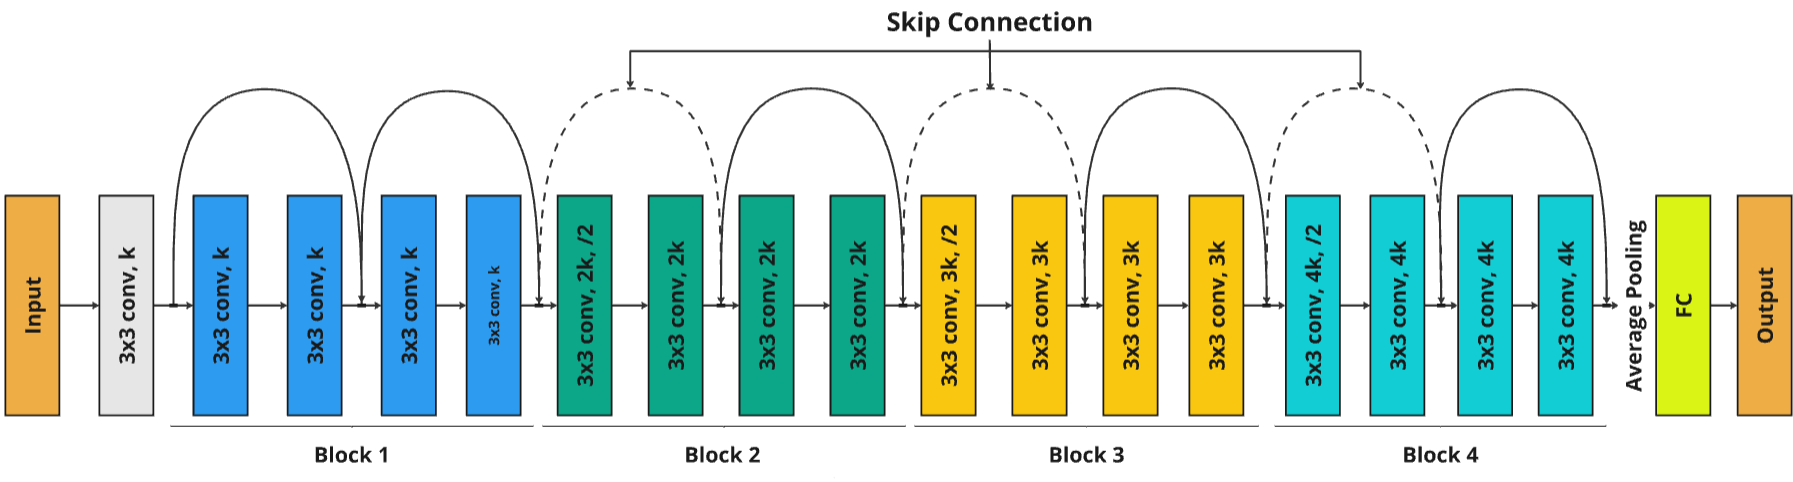
\includegraphics[width=\linewidth]{img/experiments/resnet18modified.png}
    \caption[Arquitectura ResNet$18$ modificada.]{Arquitectura ResNet$18$ modificada. Podemos observar los 4 bloques convolucionales (distinguidos por color), cada uno de ellos con su correspondiente número de filtros ([$k$, $2k$, $3k$, $4k$] con $k \in \mathbb{N}$), junto con las conexiones residuales. Imagen original del autor.}\label{fig:resnet18}
\end{figure}

La arquitectura que usaremos durante el transcurso de los experimentos es una modificación de la arquitectura ResNet$18$ original, dado que, en la arquitectura original el número de filtros usados en cada bloque convolucional es [$64$, $128$, $256$, $512$], mientras que en nuestro caso será un número variable $k \in \mathbb{N}$, con el propósito de poder modificar el número de parámetros de la red y crear ``distintas'' arquitecturas.\newline

Para ello, usaremos como número de filtros para cada bloque convolucional la secuencia: [$k$, $2k$, $3k$, $4k$]~\cite{Nakkiran2019}, con el objetivo de comparar los resultados obtenidos con los de la literatura existente. Destacamos que, para el valor $k=64$, nuestra arquitectura es la propia arquitectura ResNet-$18$ original.\newline

Finalmente y dado que el número de parámetros asociados a esta arquitectura es tedioso de indicar (debido a la gran cantidad de capas que la conforman), se expone una tabla con los principales valores del parámetro $k$ (número de filtros) utilizados en el desarrollo de la práctica (véase Tabla~\ref{tab:numero-parametrosresnet}).\newline

\begin{table}[ht]
    \centering
    \begin{tabular}{|c|c|c|}
    \hline
    \textbf{Valor de $k$}           & \textbf{Número de parámetros}                     
    \\ \hline
    $20$                  & $\approx 1.1$\space M                                            \\ \hline
    $45$                  & $\approx 5.5$\space M                                             \\ \hline
    $64$                  & $\approx 11.1$\space M                                             \\ \hline
    \end{tabular}
    \caption[Número de parámetros de las arquitecturas ResNet$18$ modificadas.]{Número de parámetros de las arquitecturas ResNet$18$ modificadas. Se muestra el número de parámetros dada un determinado valor $k$ y para $10$ clases de salida.}\label{tab:numero-parametrosresnet}
\end{table}

\subsubsection{3CNN}\label{subsubsec:3CNN}

Siguiendo la misma idea de la subsección anterior, en la que se varía el número de filtros en cada capa convolucional, se propone una nueva arquitectura compuesta por $3$ capas convolucionales (denominada $3$CNN), seguidas de capas de \textit{pooling} para reducir dimensionalidad y, finalmente, una capa densa de salida.\newline

Este modelo se presenta como una opción intermedia en términos de complejidad entre los dos modelos expuestos previamente, donde el número de filtros en cada capa se ajustará según un parámetro $k \in \mathbb{N}$, siguiendo la secuencia [$k$, $2k$, $4k$] (véase Figura~\ref{fig:3CNN}).\newline

\begin{figure}[h]
    \centering
    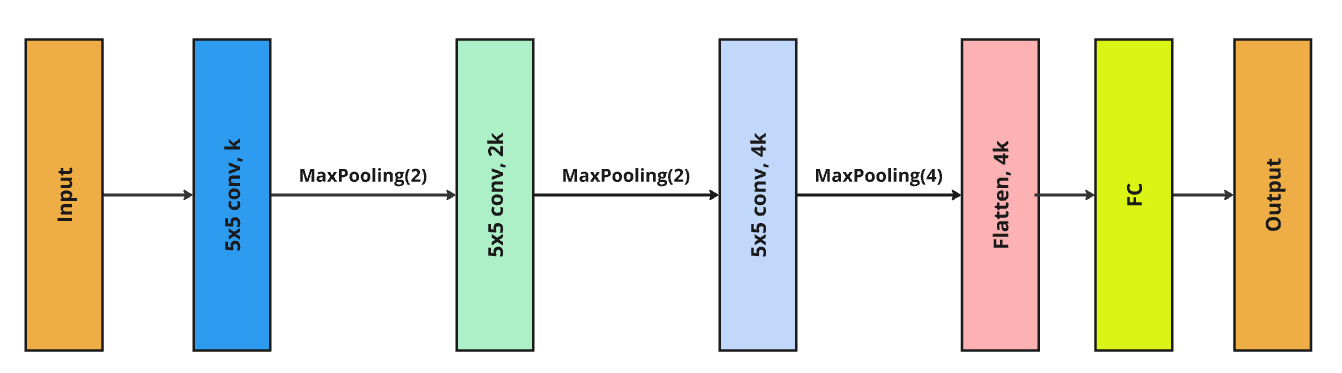
\includegraphics[width=\linewidth]{img/experiments/3CNN.png}
    \caption[Arquitectura $3$CNN.]{Arquitectura $3$CNN. Podemos observar los 3 bloques convolucionales (distinguidos por color), cada uno de ellos con su correspondiente número de filtros ([$k$, $2k$, $4k$] con $k \in \mathbb{N}$). Imagen original del autor.}\label{fig:3CNN}
\end{figure}

Finalmente, la Tabla~\ref{tab:numero-parametros3cnn} muestra el número de parámetros para algunos valores del parámetro $k$, lo que permite realizar una comparación con la arquitectura ResNet anterior.

\begin{table}[ht]
    \centering
    \begin{tabular}{|c|c|c|}
    \hline
    \textbf{Valor de $k$}           & \textbf{Número de parámetros}                     
    \\ \hline
    $20$                  & $\approx 103$\space K                                            \\ \hline
    $45$                  & $\approx 512$\space K                                             \\ \hline
    $64$                  & $\approx 1,03$\space M                                             \\ \hline
    \end{tabular}
    \caption[Número de parámetros de las arquitecturas $3$CNN.]{Número de parámetros de las $3$CNN. Se muestra el número de parámetros dada un determinado valor $k$ y para $10$ clases de salida.}\label{tab:numero-parametros3cnn}
\end{table}

\subsection{Hiperparámetros}\label{subsec:hiperparametros}

Los hiperparámetros que serán utilizados a lo largo de la experimentación, por lo general, son los valores por defecto que vienen con las implementaciones estándar de Pytorch~\cite{NEURIPS2019_9015} de los distintos métodos utilizados. Las únicas modificaciones que se han realizado son aquellas necesarias para replicar experimentos descritos en la literatura existente y, en dichos casos, se indicarán específicamente en el propio experimento.\newline

En cuanto al tamaño del lote (\textit{batch size}), variará entre $128$ y $256$, de manera similar a la literatura existente, lo que representa un valor relativamente alto, con el objetivo de acelerar el proceso de entrenamiento. Respecto a la tasa de aprendizaje del optimizador utilizado (Adam en nuestro caso), se empleará la tasa por defecto. El uso de distintos valores para \textit{batch size} y \textit{learning rate} en un problema donde se manifiesta el doble descenso se pueden observar en el Apéndice~\ref{ap:apendiceC}, donde se muestra que, si el fenómeno ocurre, el tamaño del lote utilizado y la tasa de aprendizaje no afectan significativamente al comportamiento del mismo.\newline

Por otra parte, cabe destacar que, salvo que se indique lo contrario, no se introduce ninguna técnica de regularización en los experimentos realizados, debido a que el \textit{Deep Double Descent} se observará sin la influencia de las mismas. De este modo, se pretende estudiar cómo se manifiesta este suceso bajo condiciones más puras, sin modificaciones que podrían alterar sus efectos. Cualquier variación en este aspecto será especificada de manera explícita en el propio experimento. Adicionalmente, como función de pérdida a minimizar se utilizará la entropía cruzada, dado que estamos trabajando con problemas de clasificación multiclase.\newline

\section{Experimentos}\label{sec:experimentos}

En esta sección se presentará una batería de resultados obtenidos a partir de los experimentos realizados, los cuales incluyen tanto resultados favorables como desfavorables, con el propósito de proporcionar una visión lo más completa posible de los mismos.\newline

\subsection{Aproximación polinómica de Legendre}\label{subsec:approx-legendre1}

Este primer experimento sirve como preámbulo al resto de experimentos y tiene como objetivo proporcionar una comprensión clara y sencilla de por qué puede manifestarse el \textit{Deep Double Descent} al aumentar la complejidad de un modelo. A través de este análisis preliminar, se busca sentar las bases para explorar más a fondo cómo la complejidad afecta al comportamiento y rendimiento de los modelos en los experimentos posteriores.\newline

Para ello, se busca replicar el resultado de la Imagen $2$ de~\cite{Schaeffer2023} (véase Figura~\ref{fig:1DDD}). El experimento trata de aproximar una función objetivo ($y(x) = 2x + \cos(25x)$) mediante el uso de la aproximación polinómica de Legendre para distintos grados de dicho polinomio y sobre un conjunto de $10$ puntos obtenidos al muestrear la función anterior. Este experimento no utilizará redes neuronales, sino que se basa en una simple regresión polinómica.\newline

\begin{figure}[h]
    \centering
    \begin{minipage}{0.32\textwidth}
        \centering
        \textbf{Región infraparametrizada} \\[0.5ex] 
        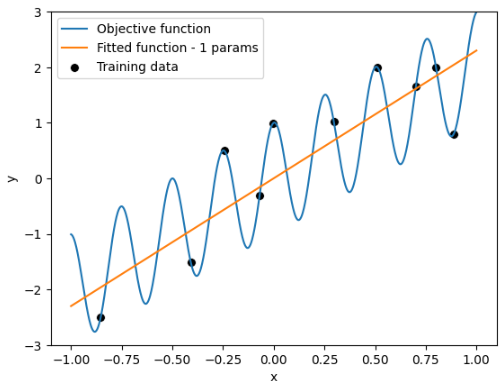
\includegraphics[width=\linewidth]{img/experiments/legendre1.png}
    \end{minipage}
    \begin{minipage}{0.32\textwidth}
        \centering
        \textbf{Umbral de interpolación} \\[0.5ex] 
        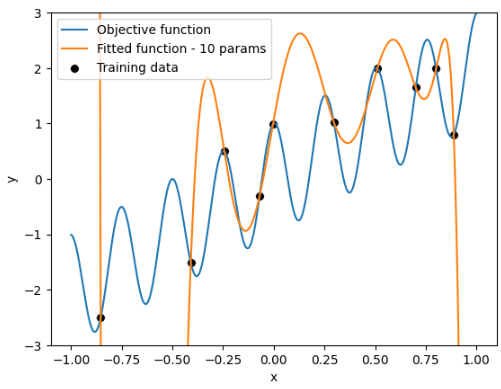
\includegraphics[width=\linewidth]{img/experiments/legendre2.png}
    \end{minipage}
    \begin{minipage}{0.32\textwidth}
        \centering
        \textbf{Región sobreparametrizada} \\[0.5ex] 
        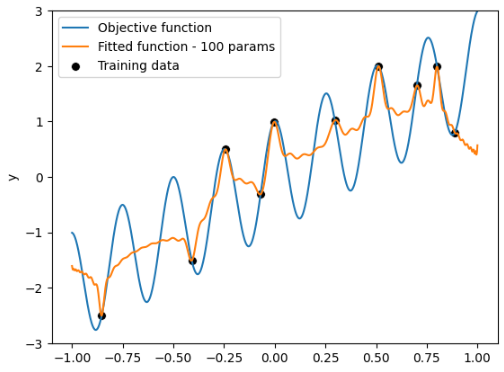
\includegraphics[width=\linewidth]{img/experiments/legendre3.png}
    \end{minipage}
    \caption[Intuición del \textit{Deep Double Descent} usando regresión polinómica.]{Intuición del \textit{Deep Double Descent} usando regresión polinómica. Cuando nos encontramos en la región infraparametrizada, el modelo no es capaz de capturar todos los datos de entrenamiento, haciendo que el bias del modelo sea grande, aunque la varianza sea pequeña. En el umbral de interpolación, el modelo captura perfectamente todos los datos, haciendo que el bias sea pequeño pero la varianza sea grande, pues la función aprendida dependerá de la posición de los datos de entrenamiento. Finalmente, en la región sobreparametrizada, el modelo está ``regularizado'' hacia una solución de norma pequeña.}\label{fig:1dd}
\end{figure}

Al alcanzar el umbral de interpolación, el modelo se ve obligado a ajustarse exactamente a cada uno de los puntos de entrenamiento, lo que lo convierte en una solución única. En este caso, el grado del polinomio coincide con el número de puntos, lo que no asegura garantizar una buena generalización debido a la ``rigidez'' del modelo al presentar numerosos ``picos'' (véase Figura~\ref{fig:1dd}).\newline

Al superar dicho umbral, el modelo adquiere mayor flexibilidad para aproximar los datos, lo que da lugar a una función cada vez más ``suave''. Además, el aumento en el número de parámetros más allá de dicho umbral permite la existencia de múltiples modelos de interpolación para cada grado, facilitando la selección de una opción que generalice bien. Esto puede observarse en la Figura~\ref{fig:1DDD}.\newline

\begin{figure}[h]
    \centering
    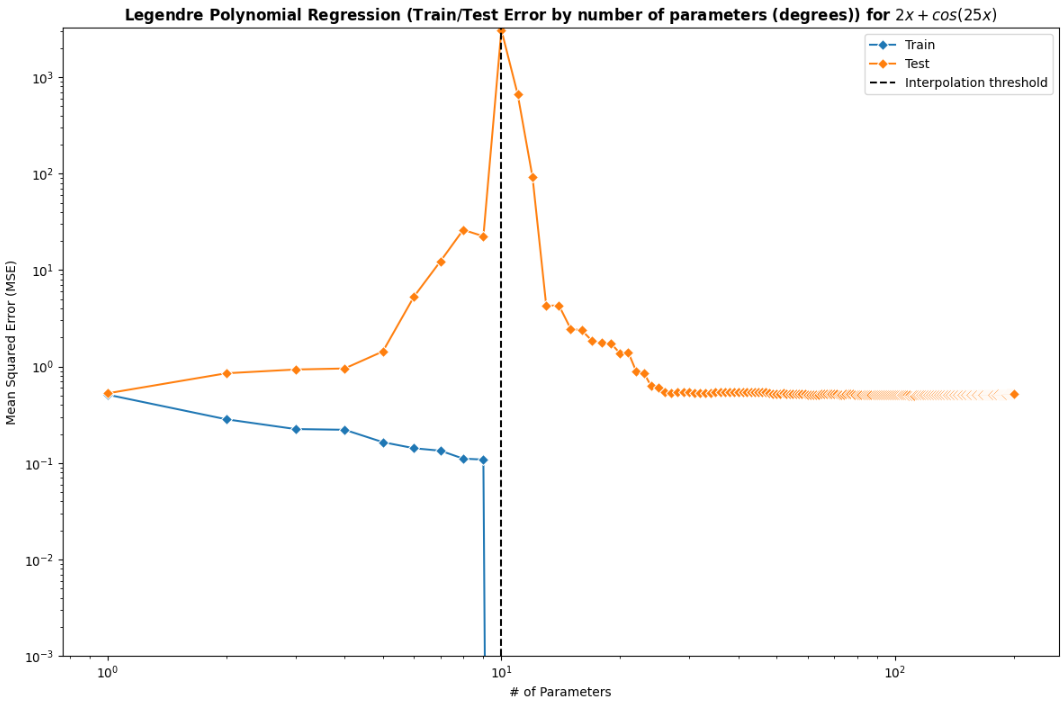
\includegraphics[width=0.5\textwidth]{img/experiments/legendreDDD.png}
    \caption[Doble descenso al utilizar aproximación polinómica de Legendre.]{Doble descenso al utilizar aproximación polinómica de Legendre, donde el umbral de interpolación corresponde al número de datos de entrenamiento.}
    \label{fig:1DDD}
\end{figure}

\subsubsection{Función cuadrática}\label{subsubsec:cuadratica}

\subsubsection{Función exponencial}\label{subsubsec:exponencial}

\subsubsection{Función hiperbólica}\label{subsubsec:hiperbolica}

\subsection{Noise-wise double descent}\label{subsec:noise-wise-dd}

En esta subsección, y como preámbulo al resto de experimentos, se estudia cómo varía el doble descenso al aumentar el porcentaje de ruido en las etiquetas. De este modo, añadimos este tipo de doble descenso a las variantes clásicas propuestas por Nakkiran et al.\ en~\cite{Nakkiran2019}.\newline

Para ello, se llevará a cabo un experimento con la arquitectura $2$NN sobre el dataset MNIST[$4000/1000$], modificando el porcentaje de ruido añadido en las etiquetas y entrenando cada modelo durante $1000$ épocas.\newline

\begin{figure}[h]
    \centering
    \begin{minipage}{0.45\textwidth}
        \centering
        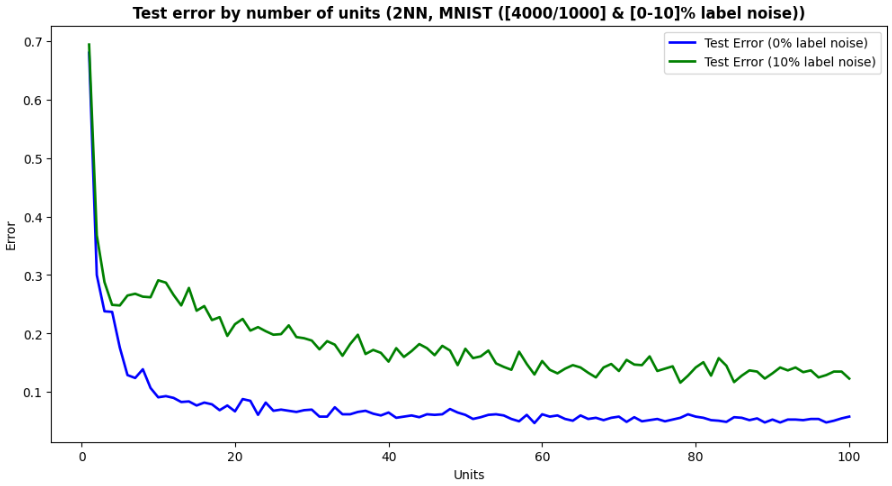
\includegraphics[width=\linewidth]{img/experiments/noise-wise-dd1.png}
    \end{minipage}
    \begin{minipage}{0.45\textwidth}
        \centering
        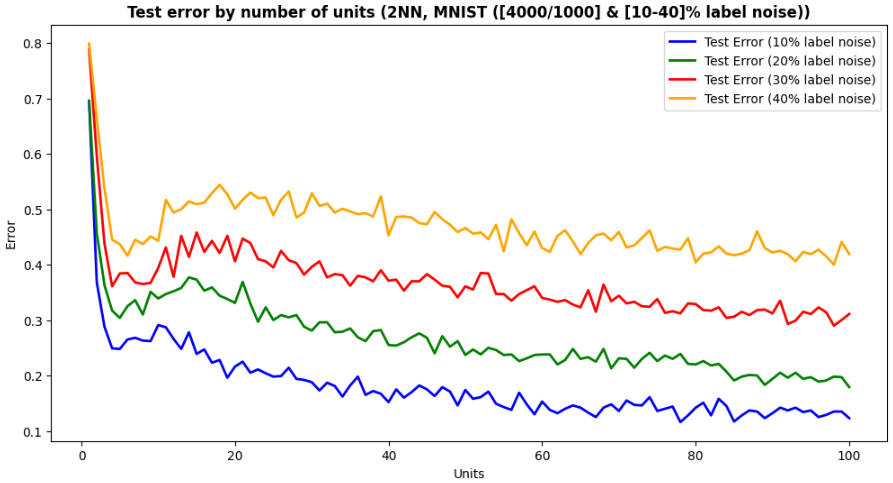
\includegraphics[width=\linewidth]{img/experiments/noise-wise-dd2.png}
    \end{minipage}
    \caption[Doble descenso para distintos niveles de ruido.]{Error en test de la arquitectura 2NN sobre el subconjunto MNIST[$4000/1000$] para diferente nivel de ruido. A la izquierda, en ausencia de ruido añadido, el doble descenso no se manifiesta. En cambio, a la derecha, al aumentar el nivel de ruido, el pico de la curva se vuelve cada vez más pronunciado.}\label{fig:noise-wise-dd}
\end{figure}

En la Figura~\ref{fig:noise-wise-dd} se observa que un modelo que no presenta doble descenso sobre el conjunto de datos original sí lo experimenta al agregarle ruido. Además, en modelos donde si aparece el doble descenso, el pico del error de test aumenta al incrementar el porcentaje de ruido, ya que el modelo, eventualmente, memorizará dicho ruido, lo cual concuerda con lo planteado en la literatura científica.\newline

También se aprecia que, a medida que aumenta el ruido, se requieren más parámetros para alcanzar errores de test más bajos que el mínimo obtenido durante el primer descenso. Este fenómeno, junto con el aumento del tiempo de entrenamiento al incrementar el ruido (véase Tabla~\ref{tab:noisewisedd}) y considerando que, en escenarios reales, el porcentaje de ruido no suele ser excesivamente alto, nos lleva a optar por configuraciones con un nivel de ruido en torno al $10-20\%$ para los experimentos restantes.\newline

Finalmente, en la Figura~\ref{fig:noise-wise-dd3} podemos verificar cómo, al aumentar el porcentaje de ruido en las etiquetas, el umbral de interpolación se desplaza hacia la derecha.\newline

\begin{figure}[h]
    \centering
    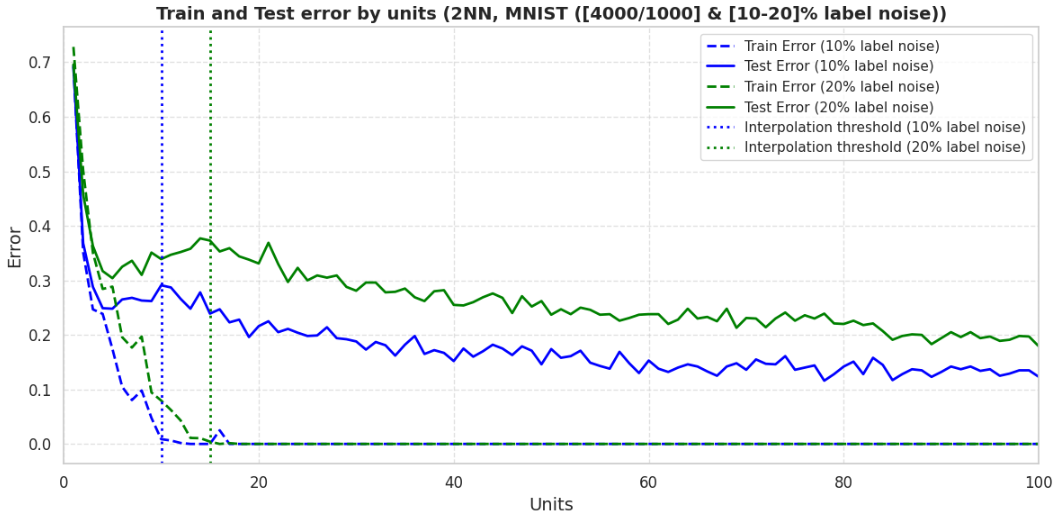
\includegraphics[width=0.5\textwidth]{img/experiments/noise-wise-dd3.png}
    \caption[Umbral de interpolación para el doble descenso con distintos niveles de ruido.]{Error en entrenamiento, test y umbral de interpolación respecto a la arquitectura $2$NN sobre el subconjunto MNIST[$4000/1000$] con distinto nivel de ruido añadido en las etiquetas.}\label{fig:noise-wise-dd3}
\end{figure}

\begin{table}[h!]
    \centering
    \begin{tabular}{|c|c|c|c|}
    \hline
    \textbf{Modelo}       & \textbf{Dataset} & \textbf{Ruido en etiquetas} & \textbf{Entrenamiento} \\ 
    \hline
    $2$-NN ($1-100$)          & MNIST[$4000/1000$]        & $\times$         & $26$h $10$min       \\ 
    $2$-NN ($1-100$)          & MNIST[$4000/1000$]        & $10\%$         & $26$h $50$min       \\ 
    $2$-NN ($1-100$)          & MNIST[$4000/1000$]        & $20\%$         & $27$h $23$min       \\ 
    $2$-NN ($1-100$)          & MNIST[$4000/1000$]        & $30\%$          & $28$h $8$min       \\ 
    $2$-NN ($1-100$)          & MNIST[$4000/1000$]       & $40\%$          & $30$h $14$min       \\  
    \hline
    \end{tabular}
    \caption[Resumen de los experimentos para el doble descenso por nivel de ruido.]{Resumen de los experimentos para el doble descenso por nivel de ruido.}
    \label{tab:noisewisedd}
    \end{table}

\subsection{Sample-wise double descent}\label{subsec:sample-wise-dd}

En esta subsección se presentan los experimentos realizados para analizar el \textit{sample-wise double descent}, el cual se manifiesta al modificar la cantidad de datos empleados durante el entrenamiento de un modelo específico. Este comportamiento destaca una zona de interés donde, al comparar las curvas del error de prueba, se observa que entrenar con un mayor número de ejemplos puede, de manera casi paradójica (en el sentido que, generalmente, en el aprendizaje automático siempre se busca tener la mayor cantidad de datos posible de cara a entrenar), empeorar el rendimiento del modelo.\newline

Dado que la experimentación presentada en la literatura existente resulta excesivamente costosa de replicar, se han diseñado experimentos más accesibles que permiten analizarlo manteniendo un enfoque lo suficientemente representativo.\newline

La idea para crear estos experimentos sencillos surge del hecho de que si un determinado modelo presenta \textit{model-wise doble descent} para un determinado número de ejemplos de entrenamiento, si aumentamos el número de ejemplos de entrenamiento, el pico del error de test se desplazará hacia la derecha (véase la imagen izquierda de la Figura~\ref{fig:swdd}), creando una región, que denominamos zona de interés.\newline

Dentro de esta zona se verifica que entrenar con más ejemplos puede empeorar el rendimiento del modelo (véase la zona sombreada en color rojo de la Figura~\ref{fig:swdd}). Sin embargo, es importante resaltar que, fuera de esta zona específica, el entrenamiento con un mayor número de ejemplos suele ser beneficioso para el rendimiento general del modelo, es decir, el modelo debería obtener menor error de test (el área bajo la curva de error fuera de dicha región debe ser menor para el modelo entrenado con un mayor número de ejemplos).\newline

Por tanto, para la realización de este experimento se utilizará la red $2$NN, donde el número de unidades de salida de la primera capa densa variará desde $1$ hasta $200$ y entrenaremos cada modelo durante $1000$ épocas. Además, se utilizará el dataset MNIST, sobre el que se extraeran $4000$ y $8000$ ejemplos para los distintos experimentos a realizar y a los que se les agregará un ruido del $10$\% en sus etiquetas.\newline

\begin{figure}[h!]
    \centering
    \begin{minipage}{0.49\textwidth}
        \centering
        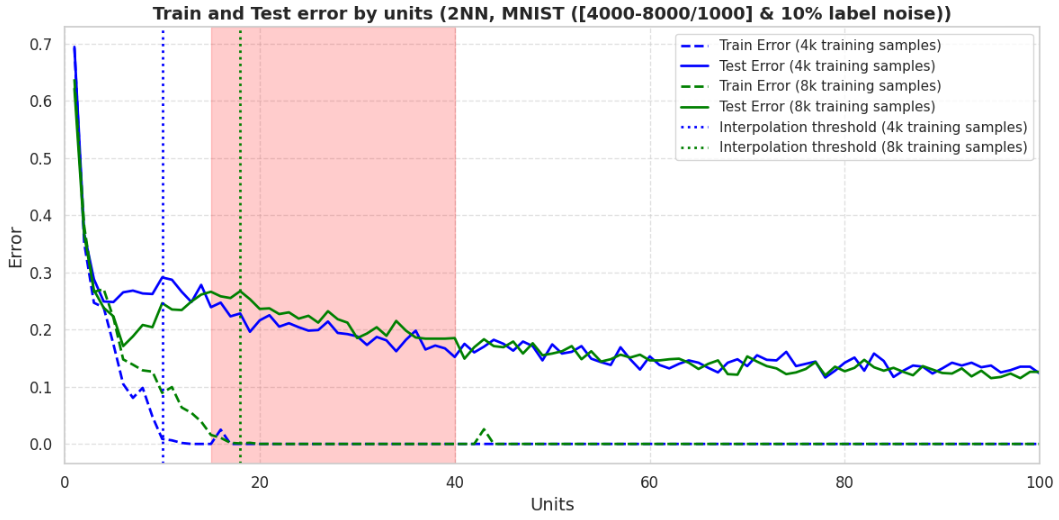
\includegraphics[width=\linewidth]{img/experiments/sample-wise-dd1.png}
    \end{minipage}
    \hfill
    \begin{minipage}{0.49\textwidth}
        \centering
        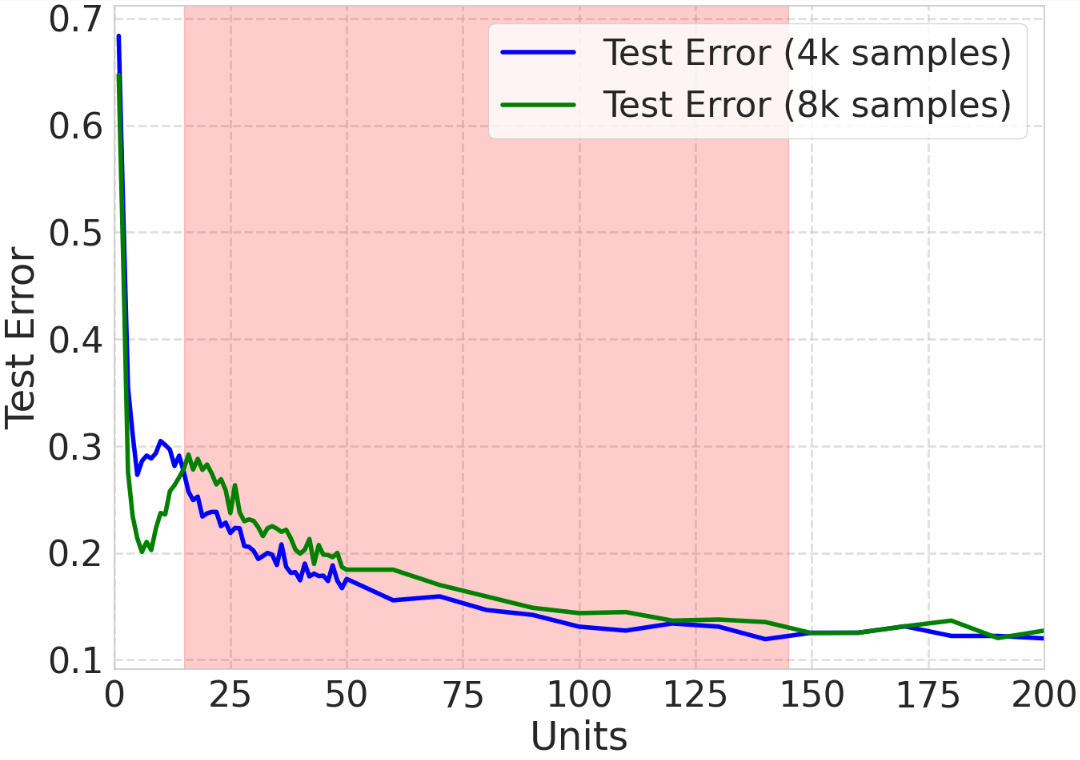
\includegraphics[width=\linewidth]{img/experiments/sample-wise-dd2.png}
    \end{minipage}
    \caption[Ejemplo de \textit{sample-wise double descent}.]{Ejemplo de \textit{sample-wise double descent} para la red $2$NN sobre dos subconjuntos de MNIST, utilizando $4000$ y $8000$ ejemplos de entrenamiento. A la izquierda aparece el resultado de una única realización del experimento. A la derecha aparece el resultado obtenido al realizar la media de $3$ experimentos.}
    \label{fig:swdd}
\end{figure}

Al igual que ocurría al aumentar el nivel de ruido, si aumentamos el número de ejemplos de entrenamiento, el umbral de interpolación también se desplaza hacia la derecha (véase la imagen izquierda de la Figura~\ref{fig:swdd}). Es decir, el modelo requiere de un mayor número de parámetros para memorizar un mayor número de ejemplos de entrenamiento, lo que, a priori, parece tener sentido con la complejidad efectiva del modelo.\newline

Finalmente, se muestra en la Tabla~\ref{tab:model_training_time} el tiempo de ejecución necesario para la realización de este experimento. Cabe destacar que, en el experimento donde se calcula la media de $3$ ejecuciones, se utiliza el modelo $2$NN hasta $50$ unidades (de $1$ en $1$) y, a partir de este valor, se suman las unidades de $10$ en $10$ hasta llegar a $200$ unidades, con el propósito de acelerar el entrenamiento fuera de la zona de interés que proporcionaba el primer experimento.\newline

\begin{table}[h!]
\centering
\begin{tabular}{|c|c|c|}
\hline
\textbf{Modelo}       & \textbf{Dataset} & \textbf{Entrenamiento} \\ 
\hline
$2$-NN ($1-100$)      & MNIST[$4000/1000$]         & $26$h $50$min       \\ 
$2$-NN ($1-100$)      & MNIST[$8000/1000$]         & $59$h       \\ 
$2$-NN ($1-200$) $\times$ $3$     & MNIST[$4000/1000$]         & $53$h $10$min       \\ 
$2$-NN ($1-200$) $\times$ $3$      & MNIST[$8000/1000$]         & $104$h $30$min       \\ 
\hline
\end{tabular}
\caption[Resumen de los experimentos para el doble descenso por número de ejemplos de entrenamiento.]{Resumen de los experimentos para el doble descenso por número de ejemplos de entrenamiento.}
\label{tab:model_training_time}
\end{table}

\section{Conclusión}\label{sec:conclusion-informatica}

\endinput

\part{Conclusiones y Trabajos Futuros}
% !TeX root = ../tfg.tex
% !TeX encoding = utf8

\chapter{Conclusiones}\label{ch:conclusiones}

La base teórica que sustenta los avances empíricos constituye una herramienta fundamental para el devenir del aprendizaje automático, y su desarrollo resulta esencial para comprender los nuevos comportamientos que van surgiendo en este ámbito. En el presente TFG, nos enfocamos en dar explicación al \textit{Deep Double Descent} a partir del desarrollo de nuevos conceptos dentro del aprendizaje, unificando la sabiduría clásica con la experimentación moderna.

En primer lugar, se realizó un análisis exhaustivo del estado del arte relacionado con las distintas manifestaciones del suceso, constatando su novedosa y creciente relevancia en la comunidad científica, así como identificando sus principales desencadenantes tanto en problemas de regresión como de clasificación.

A continuación, nos centramos en revisar conceptos básicos de probabilidad y álgebra lineal, especialmente aquellos relativos a matrices, necesarios para introducir los fundamentos clásicos del aprendizaje. A su vez, estos conocimientos constituyen la base teórica sobre la que también se construyen y formalizan gran parte de los conceptos del aprendizaje moderno.

Posteriormente, nos adentramos en el estudio clásico del \textit{deep learning}, presentando los principales problemas que este paradigma busca resolver y centrándonos especialmente en tareas de regresión y procesamiento de imágenes mediante redes neuronales convolucionales (CNNs). Esta etapa sirve como preámbulo para abordar el dilema clásico del aprendizaje, permitiendo establecer un marco coherente que conecta los fundamentos estadísticos con los desafíos inherentes en este campo.

Una vez definido el concepto de aprendizaje, nos centramos en desarrollar los principales conceptos clásicos asociados, los cuales constituyen su base teórica fundamental. Esta revisión permitió establecer de forma precisa el marco teórico tradicional, sirviendo de punto de partida para comprender las diferencias y desafíos que surgen en el marco del aprendizaje moderno. De igual manera, nos permitió profundizar en la comprensión de conceptos clásicos de generalización, revelando metodologías de utilidad para el estudio de nuestro problema.

El núcleo del proyecto se centra en la exposición del \textit{Deep Double Descent} desde una perspectiva tanto teórica como empírica. Inicialmente, se establece un planteamiento teórico del mismo, resolviendo sus discrepancias con la teoría clásica y realizando un análisis intuitivo de su aparición en problemas de regresión. Posteriormente, se presentan resultados que corroboran su aparición al emplear el descenso de gradiente como método de optimización. 

Por otro lado, se realiza un estudio exhaustivo en la zona de sobreparametrización, donde se obtienen resultados que permiten aclarar su aparición desde un punto de vista teórico, a partir de la definición de sesgos inductivos que guían al modelo hacia soluciones efectivas, fundamentadas en su simplicidad, y que amplían la comprensión más allá de lo que la teoría clásica puede proporcionar, ofreciendo nuevos límites de generalización.

Para finalizar la parte teórica, se introducen conceptos de la aproximación no lineal, estrechamente ligados al concepto del aprendizaje y al propio fenómeno, destacando el uso de distintas bases y diccionarios redundantes de funciones, lo que proporciona una nueva perspectiva para su interpretación.

Para finalizar el proyecto, se lleva a cabo la constatación experimental de los resultados teóricos expuestos. En primer lugar, se comprueba que, al abordar problemas de regresión, la elección de la base utilizada desempeña un papel fundamental en la calidad de las sucesivas aproximaciones. Por otro lado, en tareas de clasificación de imágenes, se observa cómo el fenómeno emerge en contextos típicos del aprendizaje automático, especialmente cuando el modelo supera de largo su capacidad efectiva, ya sea por exceso de parámetros o al realizar el entrenamiento durante un tiempo excesivo. Asimismo, se corrobora que el ruido desempeña un papel crucial tanto en su aparición como en su intensidad.

Por ende, el presente trabajo ha establecido una base sólida para comprender el \textit{Deep Double Descent}. Además, actúa como un puente entre los enfoques clásicos y modernos, ofreciendo una primera aproximación hacia el mundo de la generalización en escenarios de sobreparametrización. No obstante, aún existe un amplio margen para descubrir principios subyacentes a este comportamiento y explorar sus posibles manifestaciones y su relevancia en diversos problemas del mundo actual.

Para el desarrollo de este TFG se han aplicado conocimientos adquiridos en asignaturas como Aprendizaje Automático, Aprendizaje Profundo, Visión por Computador, Probabilidad y Geometría. Además, se han conseguido nuevos conocimientos relacionados con la Aproximación No Lineal, conceptos clásicos y nuevas teorías del Aprendizaje Profundo, así como el uso práctico de herramientas y métodos basados en la biblioteca \textit{PyTorch}.

A modo de conclusión, podemos asegurar que los objetivos presentados al inicio del trabajo se han cumplido de manera satisfactoria, cumpliendo con las expectativas establecidas. No obstante, como se detallará en la siguiente sección, han surgido diversas oportunidades para futuras investigaciones, impulsadas tanto por la naturaleza innovadora de este estudio como por las restricciones de tiempo y recursos computacionales.

\chapter{Trabajos futuros}\label{ch:trabajos-futuros}

Aunque nuestro trabajo ha representado un avance significativo en la comprensión de nuevas dinámicas de actuación de las arquitecturas profundas, especialmente en términos de generalización, aún existen diversos aspectos que requieren un análisis más profundo. Ligado a esto se suma el carácter emergente y en constante evolución de este campo dentro de la IA, que invita a seguir explorando nuevas hipótesis y enfoques que permitan construir un conocimiento más sólido de estos comportamientos.

En primer lugar, una línea de trabajo evidente sería profundizar en experimentos más ambiciosos que no hemos podido llevar a cabo debido a limitaciones en la capacidad de cómputo. Para ello, se propone emplear arquitecturas con una capacidad extremadamente mayor y entrenarlas durante un período de tiempo más prolongado, con el fin de corroborar que, en la mayoría de los casos, se alcanzarán errores inferiores a los del primer descenso. Más aún, sería interesante explorar el uso de otro tipo de arquitecturas de gran escala, tales como los \textit{Transformers} o modelos basados en técnicas de \textit{ensembling}.

Por otra parte, sería interesante indagar en la relación entre el \textit{Deep Double Descent} y el \textit{Grokking}, dado que ambos parecen representar un mismo escenario en términos de generalización en modelos sobreparametrizados. De esta manera, se podría avanzar hacia la unificación de las nuevas tendencias emergentes en el mundo de la generalización dentro de un marco teórico común.

Otra línea de investigación con gran potencial consistiría en llevar a cabo un análisis preliminar del problema a abordar, con el objetivo de estimar de forma anticipada el tiempo y la capacidad computacional necesarios para alcanzar mejoras en el rendimiento durante el segundo descenso. De este modo, se buscaría desarrollar una herramienta capaz de predecir el coste estimado necesario para producir mejoras de rendimiento con respecto a las del mínimo alcanzado durante el descenso clásico inicial. 

Volviendo a los experimentos, sería razonable estudiar el comportamiento del suceso ante datos que incluyan distintos tipos de ruido, no solo en las etiquetas, sino también en las propia entrada. Esto permitiría observar cómo se comporta el suceso frente a distintos escenarios que pueden presentarse en el mundo real, dado que el ruido en estos entornos no sigue, por lo general, una distribución uniforme.

Un campo adicional de exploración consistiría en estudiar el comportamiento del fenómeno en problemas de regresión que utilicen modelos neuronales, con el objetivo de verificar si existen matices o diferencias en comparación con los problemas de clasificación. Además, en estos escenarios, sería interesante explorar un mayor número de bases para la aproximación y estudiar las razones por las cuales ciertas bases pueden presentar el doble descenso mientras que otras no lo hacen.

Como se ha mencionado anteriormente, existe un amplio margen de mejora, especialmente en el ámbito empírico. Sin embargo, el estudio del \textit{Deep Double Descent} ha arrojado luz sobre la explicabilidad de la generalización en la actualidad. Este suceso pone de manifiesto la importancia de no ignorar estas nuevas tendencias, sino de trabajar para conseguir una integración con los enfoques tradicionales, con el objetivo de sentar las bases que permitan unificar los avances recientes con los fundamentos clásicos.

\endinput

% Añadir tantos capítulos como sea necesario

% \cleardoublepage\part{Segunda parte}
% \input{capitulos/capitulo-ejemplo}

% -------------------------------------------------------------------
% APPENDIX: Opcional
% -------------------------------------------------------------------

\appendix % Reinicia la numeración de los capítulos y usa letras para numerarlos
\pdfbookmark[-1]{Apéndices}{appendix} % Alternativamente podemos agrupar los apéndices con un nuevo \part{Apéndices}

% !TeX root = ../tfg.tex
% !TeX encoding = utf8

\chapter{Detalles Matemáticos Adicionales}\label{ap:apendiceA}

En este apéndice se muestran la demostraciones del Lema~\ref{lema:raro-clasificación-gd}, extraída de~\cite{Soudry2024} y de la Proposición~\ref{prop:non-conexity}.\newline

\textbf{Lema}~\ref{lema:raro-clasificación-gd}. Sea $\mathcal{L}(w)$ una función $\beta$-suave no negativa. Si $\eta < \frac{2}{\beta}$, entonces, para cualquier $w_0$ y utilizando el método del descenso de gradiente dado por:

\[
    w^{(\tau + 1)} = w^{(\tau)} - \eta \nabla \mathcal{L}(w)
\]

se tiene que $\sum_{u=0}^{\infty} \| \nabla\mathcal{L}(w^{(u)}) \|^{2} < \infty$ y, por tanto:

\[
    \lim \limits_{t \to \infty} \| \nabla\mathcal{L}(w^{(t)}) \|^{2} = 0.
\]

\begin{proof}
  Usando una propiedad conocida de las funciones $\beta$-suaves:

  \[
      | f(x) - f(y) - \nabla f(y)^{T} (x-y) | \leq \| x - y \|^2.
  \]  

  Dado que la función $\mathcal{L}(w)$ es $\beta$-suave:

  \begin{align}
      \mathcal{L} (w^{(\tau + 1)}) &\leq \mathcal{L} (w^{(\tau)}) + \nabla \mathcal{L} (w^{\tau})^{T} (w^{(\tau + 1)} - w^{\tau}) + \frac{\beta}{2} \|w^{(\tau + 1)} - w^{(\tau)}\|^2 \notag \\
      &= \mathcal{L} (w^{(\tau)}) - \eta \|\nabla \mathcal{L} (w^{(\tau)})\|^2 + \frac{\beta \eta^2}{2} \|\nabla \mathcal{L} (w^{(\tau)})\|^2 \notag \\
      &= \mathcal{L} (w^{(\tau)}) - \eta \left( 1 - \frac{\beta \eta}{2} \right) \|\nabla \mathcal{L} (w^{(\tau)})\|^2.
  \end{align}

  Así, tenemos:

  \[
      \frac{\mathcal{L} (w^{(\tau)}) - \mathcal{L} (w^{(\tau + 1)})}{\eta \left( 1 - \frac{\beta \eta}{2} \right)} \geq \|\nabla \mathcal{L} (w^{(\tau)})\|^2
  \]

  lo que implica

  \[
      \sum_{u=0}^{t} \|\nabla \mathcal{L} (w^{(u)})\|^2 \leq \sum_{u=0}^{t} \frac{\mathcal{L} (w^{(u)}) - \mathcal{L} (w^{(u+1)})}{\eta \left( 1 - \frac{\beta \eta}{2} \right)} = \frac{\mathcal{L} (w_0) - \mathcal{L} (w^{(\tau + 1)})}{\eta \left( 1 - \frac{\beta \eta}{2} \right)}.
  \]

  El lado derecho está acotado por una constante finita, dado que $\mathcal{L} (w_0) < \infty$ y $0 \leq \mathcal{L} (w^{(\tau + 1)})$. Por tanto, esto implica que

  \[
      \sum_{u=0}^{\infty} \|\nabla \mathcal{L} (w^{(u)})\|^2 < \infty,
  \]

  y, finalmente, nos queda el resultado buscado: $\|\nabla \mathcal{L} (w^{(\tau)})\|^2 \to 0$.
\end{proof}

\textbf{Proposición}~\ref{prop:non-conexity}. Sea $w^{*}$ una solución, es decir, $\mathcal{L}(w^{*}) = 0$, y supongamos que $\frac{d}{dw}\frac{\partial \mathcal{L}}{\partial \mathcal{F}}(w^{*}) \neq 0$ y $rang(H_{\mathcal{F}_{i}}(w^{*})) > 2n$ para algún $i \in \{1, \ldots, n \}$. Entonces $\mathcal{L}(w)$ no es convexa en ninguna vecindad de $w^{*}$.

\begin{proof}
    La matriz Hessiana de una función de pérdida $\mathcal{L}(\mathcal{F}(w))$ viene dada por:

    \[
        H_{\mathcal{L}}(w) = D\mathcal{F}(w)^T \frac{\partial^2 \mathcal{L}}{\partial \mathcal{F}^2}(w) D\mathcal{F}(w) + \sum_{i=1}^{n} \frac{\partial \mathcal{L}}{\partial \mathcal{F}_i}(w) H_{\mathcal{F}_i}(w).
    \]

    Consideramos ahora las matrices Hessianas de dos puntos $w^* + \delta $ y $w^* - \delta $ $(\delta \in \mathbb{R}^{P})$ que están en una vecindad suficientemente pequeña de $w^*$. La Hessiana de la función de pérdida en estos dos puntos es:

    \begin{equation}\label{eq:non-convexity1}
        \begin{aligned}
            H_{\mathcal{L}}( w^* + \delta) &=  
            \underbrace{D\mathcal{F}( w^* + \delta)^T \frac{\partial^2 \mathcal{L}}{\partial \mathcal{F}^2}( w^* + \delta) D\mathcal{F}( w^* + \delta)}_{A( w^* + \delta)} \\
            &\quad + \sum_{i=1}^{n} \left( \frac{d}{d w} \left( \frac{\partial \mathcal{L}}{\partial \mathcal{F}}( w^*) \right) \delta \right)_i H_{\mathcal{F}_i}( w^* + \delta) + o(\|\delta\|),
        \end{aligned}
    \end{equation}
        
    \begin{align}
        H_{\mathcal{L}}( w^* - \delta) &=  
        \underbrace{D\mathcal{F}( w^* - \delta)^T \frac{\partial^2 \mathcal{L}}{\partial \mathcal{F}^2}( w^* - \delta) D\mathcal{F}( w^* - \delta)}_{A( w^* - \delta)} \nonumber \\
        &\quad - \sum_{i=1}^{n} \left( \frac{d}{d w} \left( \frac{\partial \mathcal{L}}{\partial \mathcal{F}}( w^*) \right) \delta \right)_i H_{\mathcal{F}_i}( w^* + \delta) + o(\|\delta\|).
    \end{align}
        

    donde los términos $ A( w^* + \delta) $ y $ A( w^* - \delta) $ son matrices de rango a lo sumo $ n $, ya que $ D\mathcal{F} $ es de tamaño $ n \times m $ ($o(\|\delta\|)$ representa un término asintóticamente menor que $\| \delta \|$).\newline

    Sabemos que al menos un componente $ H_{\mathcal{F}_k} $ de la matriz Hessiana de $ \mathcal{F} $ satisface que el rango de $ H_{\mathcal{F}_k}( w^*) $ es mayor que $ 2n $. Por continuidad de la Hessiana, si el orden de $ \delta $ es suficientemente pequeño, entonces los rangos de $ H_{\mathcal{F}_k}( w^* + \delta) $ y $ H_{\mathcal{F}_k}( w^* - \delta) $ también son mayores que $ 2n $. Esto nos lleva a que siempre podemos encontrar un vector unitario $v \in \mathbb{R}^P $ que cumpla:

    \[
        v^T A( w^* + \delta)  v =  v^T A( w^* - \delta)  v = 0.
    \]

    Sin embargo, dicho vector también verifica:

    \[
        v^T H_{\mathcal{F}_k}( w^* + \delta)  v \neq 0, \quad  v^T H_{\mathcal{F}_k}( w^* - \delta)  v \neq 0.
    \]\newline

    De esta manera, el vector $ \langle v^T H_{\mathcal{F}_1}( w^*+\delta)  v, \dots,  v^T H_{\mathcal{F}_n}( w^*+\delta)  v \rangle \neq 0$. El mismo resultado se verifica para el punto $w^* - \delta$. Así, utilizando este vector $v$ en la Hessiana de la función de pérdida en los dos puntos tenemos:

    \begin{align}
        v^T H_{\mathcal{L}}( w^* + \delta)v &=  
        \sum_{i=1}^{n} \left( \frac{d}{d w} \left( \frac{\partial \mathcal{L}}{\partial \mathcal{F}}( w^*) \right) \delta \right)_i v^T H_{\mathcal{F}_i}( w^* + \delta) v + o(\|\delta\|),
    \end{align}

    \begin{align}
        v^T H_{\mathcal{L}}( w^* - \delta)v &=  
        - \sum_{i=1}^{n} \left( \frac{d}{d w} \left( \frac{\partial \mathcal{L}}{\partial \mathcal{F}}( w^*) \right) \delta \right)_i v^T H_{\mathcal{F}_i}( w^* - \delta) v + o(\|\delta\|).
    \end{align}

    Para finalizar tenemos que mostrar que, para un $\delta$ suficientemente pequeño, $v^T H_{\mathcal{L}}(w^* + \delta) v$ y $v^T H_{\mathcal{L}}(w^* - \delta) v$ no pueden ser simultáneamente no negativos, lo que implica inmediatamente que $H_{\mathcal{L}}$ no es semidefinida positiva en una vecindad cercana de $w^*$, y por tanto, $\mathcal{L}$ no es localmente convexa en $w^*$. Usando la condición 
    \[
    \frac{d}{dw} (\frac{\partial \mathcal{L}}{\partial \mathcal{F}}(w^*)) = 0,
    \]
    para las ecuaciones anteriores, se presentan los siguientes casos:\newline

    \textbf{Caso 1:} Si 
    \[
    \sum_{i=1}^{n} \left( \frac{d}{dw} (\frac{\partial \mathcal{L}}{\partial \mathcal{F}}(w^*))\delta \right)_i v^T H_{\mathcal{F}_i}(w^* + \delta) v < 0,
    \]
    entonces, directamente, $v^T H_{\mathcal{L}}(w^* + \delta) v < 0$ si $\delta$ es lo suficientemente pequeño.\newline

    \textbf{Caso 2:} De lo contrario, si 
    \[
    \sum_{i=1}^{n} \left( \frac{d}{dw} (\frac{\partial \mathcal{L}}{\partial \mathcal{F}}(w^*))\delta \right)_i v^T H_{\mathcal{F}_i}(w^* + \delta) v > 0,
    \]
    por la continuidad de cada $H_{\mathcal{F}_i}(\cdot)$, tenemos que
    \[
        -\sum_{i=1}^{n} \left( \frac{d}{dw} (\frac{\partial \mathcal{L}}{\partial \mathcal{F}}(w^*))\delta \right)_i v^T H_{\mathcal{F}_i}(w^* - \delta) v
    \]

    \[
        \\ = -\sum_{i=1}^{n} \left( \frac{d}{dw} (\frac{\partial \mathcal{L}}{\partial \mathcal{F}}(w^*))\delta \right)_i v^T H_{\mathcal{F}_i}(w^* + \delta) v + \sum_{i=1}^{n} \left( \frac{d}{dw} (\frac{\partial \mathcal{L}}{\partial \mathcal{F}}(w^*))\delta \right)_i v^T (H_{\mathcal{F}_i}(w^* + \delta) v - \mathcal{H}_{\mathcal{F}_i}(w^* - \delta)) v
    \]

    \[
        \\ = -\sum_{i=1}^{n} \left( \frac{d}{dw} (\frac{\partial \mathcal{L}}{\partial \mathcal{F}}(w^*))\delta \right)_i v^T H_{\mathcal{F}_i}(w^* + \delta) v + O(\epsilon) < 0,
    \]
    
    cuando $\delta$ es lo suficientemente pequeño. A modo de conclusion, dado un $\delta$ arbitrariamente pequeño, se tiene que $v^T H_{\mathcal{L}}(w^* + \delta) v$ o $v^T H_{\mathcal{L}}(w^* - \delta) v$ es negativo, lo que significa que $\mathcal{L}(w)$ no tiene ninguna vecindad convexa alrededor de $w^*$.

\end{proof}

\endinput
%------------------------------------------------------------------------------------
% FIN DEL APÉNDICE. 
%------------------------------------------------------------------------------------

% !TeX root = ../tfg.tex
% !TeX encoding = utf8

\chapter{Experimentos Adicionales: Hiperparámetros}\label{ap:apendiceB}

En este apéndice se presentan dos experimentos relacionados con el uso de diferentes tamaños de lote y tasas de aprendizaje para un modelo que exhibe el doble descenso, con la finalidad de verificar su comportamiento ante distintas configuraciones. Para ello, se empleará la arquitectura $2$NN sobre el subconjunto MNIST[$4000/1000$], al cual se le añadirá un porcentaje variable de ruido, y donde se utilizarán distintas tasas de aprendizaje.
 
\subsection*{Double descent con distinto tamaño de batch}

\begin{figure}[h!]
    \centering
    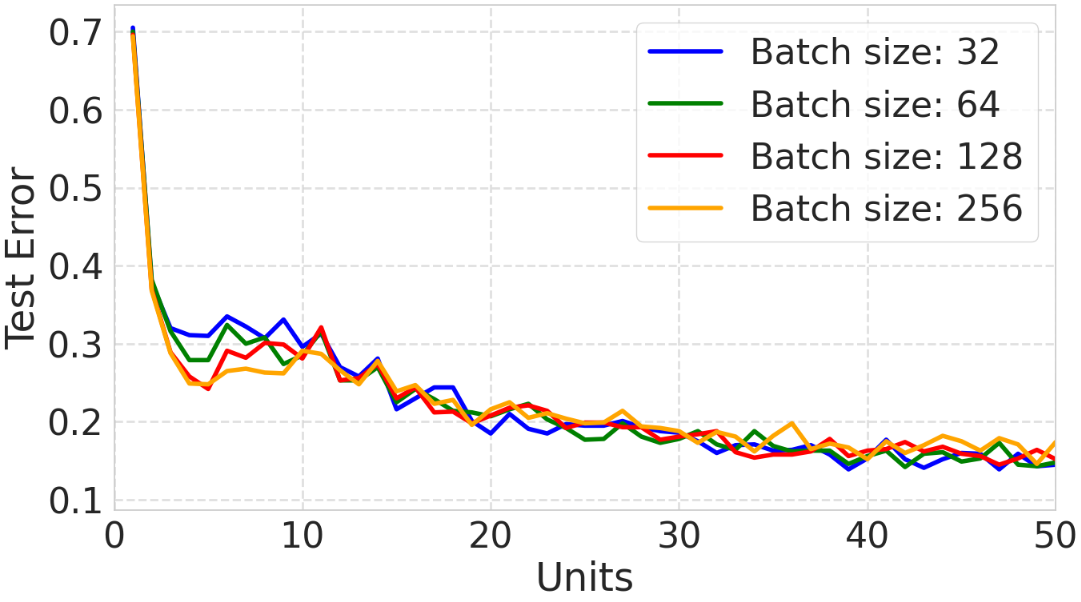
\includegraphics[width=0.65\textwidth]{img/experiments/batch_sizes_ddd.png}
    \caption[Doble descenso para distintos tamaños de lote.]{Error en test respecto a distintas configuraciones de tamaño de batch de la red $2$NN sobre el subconjunto MNIST[$4000/1000$] con $10$\% de ruido añadido.}\label{fig:dddbatchsizes}
\end{figure}

En la Figura~\ref{fig:dddbatchsizes} se observa que, para distintas configuraciones de tamaño de batch, se manifiesta el doble descenso, siendo más notable (sin tantos altibajos en la curva del error) al utilizar tamaños de lote mayores, debido a que se utiliza un mayor número de ejemplos para actualizar los parámetros en cada iteración. Por otro lado, la Tabla~\ref{tab:dddbatchsizes} muestra que, al incrementar el tamaño de batch, el tiempo de entrenamiento disminuye, lo cual es lógico, ya que se procesan un mayor número de ejemplos en cada iteración. Por tanto, considerando ambos resultados, se concluye que utilizar un tamaño de lote elevado ($128$ o $256$) es la opción adecuada para los distintos experimentos a realizar, ya que permite observar el fenómeno de forma más precisa y con menor coste computacional.

\begin{table}[h!]
    \centering
    \begin{tabular}{|c|c|c|c|}
    \hline
    \textbf{Modelo}       & \textbf{Dataset} & \textbf{Batch size} & \textbf{Entrenamiento} \\ 
    \hline
    $2$NN ($1-50$)     & MNIST[$4000/1000 - 10$\% noise]      & $32$      & $15$h $2$min         \\ 
    $2$NN ($1-50$)     & MNIST[$4000/1000 - 10$\% noise]      & $64$      & $11$h $56$min         \\ 
    $2$NN ($1-50$)     & MNIST[$4000/1000 - 10$\% noise]      & $128$      & $11$h $14$min         \\ 
    $2$NN ($1-50$)     & MNIST[$4000/1000 - 10$\% noise]      & $256$      & $10$h $23$min         \\
    \hline
    \end{tabular}
    \caption[Resumen de los experimentos realizados para el doble descenso con distinto tamaño de lote.]{Resumen de los experimentos realizados para el doble descenso con distinto tamaño de lote.}\label{tab:dddbatchsizes}
\end{table}

\subsection*{Double descent con distinto learning rate}

\begin{figure}[h!]
    \centering
    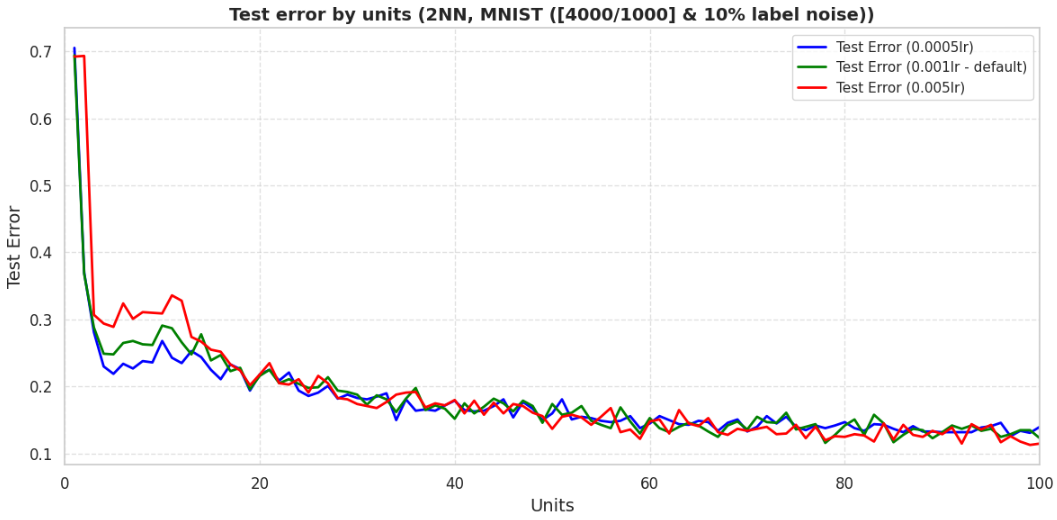
\includegraphics[width=0.65\textwidth]{img/experiments/learning_rates_ddd.png}
    \caption[Doble descenso para distinto \textit{learning rate}.]{Error en test respecto a distintas configuraciones de \textit{learning rate} obtenido por la red $2$NN sobre el subconjunto MNIST[$4000/1000$] con $10$\% de ruido añadido.}\label{fig:difflr}
\end{figure}

En la Figura~\ref{fig:difflr} podemos observar cómo se manifiesta el doble descenso para distintas configuraciones de la tasa de aprendizaje. En particular, el pico del error de test se hace más pronunciado a medida que la tasa de aprendizaje aumenta, dado que para un \textit{learning rate} igual a $5 \times 10^{-4}$, el máximo error en test es mayor que para el valor por defecto de la tasa de aprendizaje ($10^{-4}$) del optimizador Adam, y este, a su vez, es mayor que el máximo valor que proporciona la mínima tasa de aprendizaje utilizada ($5 \times 10^{-5}$).

En conclusión, esto nos indica que, si un modelo presenta el doble descenso, no es necesario preocuparse en exceso por ajustar de manera precisa la tasa de aprendizaje, puesto que, dentro de ciertos rangos de valores de este hiperparámetro, el modelo sigue presentando el suceso, lo que indica que el uso por defecto de la tasa de aprendizaje resulta ser suficiente.

Finalmente, para concluir esta subsección se muestra en la Tabla~\ref{tab:difflr} un resumen de los experimentos realizados junto con sus respectivos tiempos de entrenamiento.

\begin{table}[h!]
    \centering
    \begin{tabular}{|c|c|c|c|}
    \hline
    \textbf{Modelo}       & \textbf{Dataset} & \textbf{Tasa aprendizaje} & \textbf{Entrenamiento} \\ 
    \hline
    $2$NN ($1-100$)     & MNIST[$4000/1000 - 10$\% noise]      & $0.005$      & $23$h $53$min         \\ 
    $2$NN ($1-100$)     & MNIST[$4000/1000 - 10$\% noise]      & $0.001$ (default)      & $26$h $50$min     \\ 
    $2$NN ($1-100$)     & MNIST[$4000/1000 - 10$\% noise]      & $0.0005$      & $27$h $32$min         \\ 
    \hline
    \end{tabular}
    \caption[Resumen de los experimentos realizados para el doble descenso con distinto \textit{learning rate}.]{Resumen de los experimentos realizados para el doble descenso con distinto \textit{learning rate}.}\label{tab:difflr}
\end{table}

\endinput
%------------------------------------------------------------------------------------
% FIN DEL APÉNDICE. 
%------------------------------------------------------------------------------------

% !TeX root = ../tfg.tex
% !TeX encoding = utf8

\chapter{Irregularidades en la Dinámica del Error}\label{ap:apendiceC}

En este apéndice analizamos en detalle los saltos bruscos que se producen tanto en el error de entrenamiento como en el de prueba al aumentar el número de épocas de un determinado modelo, e intentamos proporcionar una explicación para los mismos.\newline

Nos centramos en la gráfica de la Figura~\ref{fig:model-epoch3CNNCIFAR10}, donde estos picos en el error son más sobresalientes. A partir de esta representación, se analiza el \textit{epoch-wise double descent} en dos modelos que la conforman: uno infraparametrizado, ubicado antes del umbral de interpolación, y otro sobreparametrizado, situado después de dicho umbral.\newline

\begin{figure}[h]
    \centering
    \begin{subfigure}[b]{\textwidth}
        \centering
        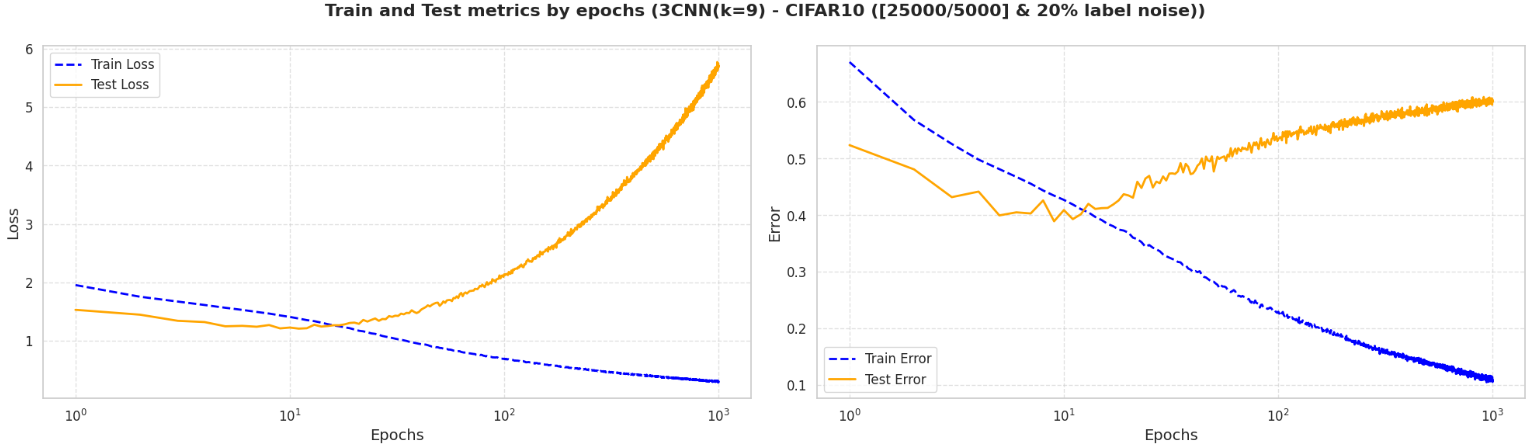
\includegraphics[width=0.7\textwidth]{img/experiments/epoch-wise3CNNunderparameterized.png}
        \caption{A la izquierda, se muestra la pérdida en entrenamiento y prueba, y a la derecha, el error en entrenamiento y prueba para un modelo $3$CNN infraparametrizado sobre el subconjunto CIFAR$10$[$25000/5000$].}\label{fig:epoch-wise3CNNunderparameterized}
    \end{subfigure}
    
    \vspace{1em} 

    \begin{subfigure}[b]{\textwidth}
        \centering
        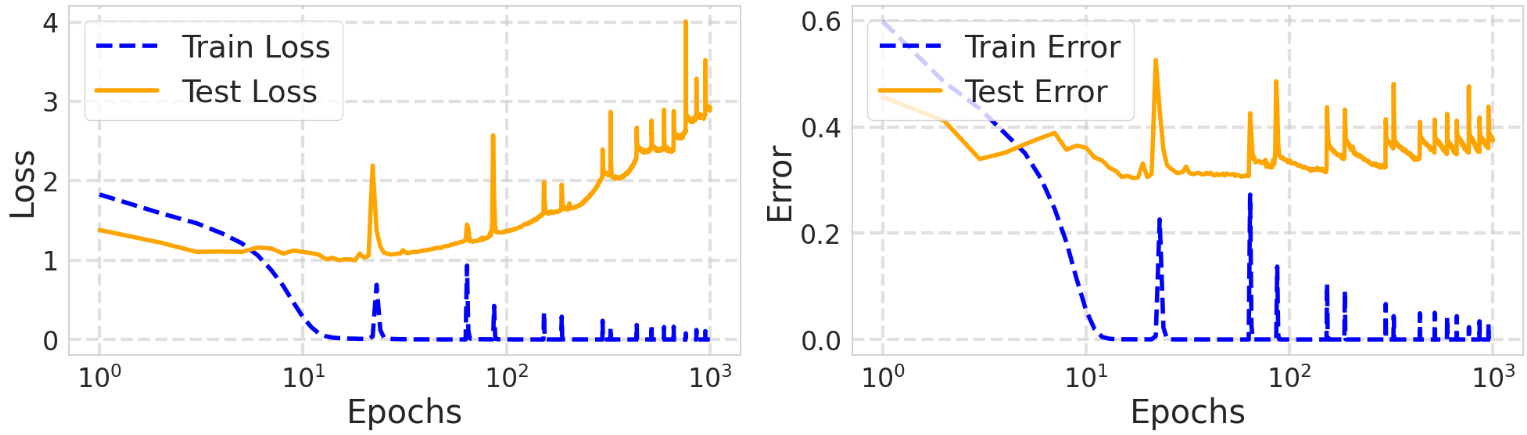
\includegraphics[width=0.7\textwidth]{img/experiments/epoch-wise3CNNoverparameterized.png}
        \caption{A la izquierda, se muestra la pérdida en entrenamiento y prueba, y a la derecha, el error en entrenamiento y prueba para un modelo $3$CNN sobreparametrizado sobre el subconjunto CIFAR$10$[$25000/5000$], donde se aprecian variaciones abruptas tanto en la gráfica de la pérdida como en la del error.}\label{fig:epoch-wise3CNNoverparameterized}
    \end{subfigure}
    
    \caption[Comparativa \textit{epoch-wise double descent} entre un modelo infraparametrizado y uno sobreparametrizado en el que aparecen picos significativos en el error.]{Comparativa \textit{epoch-wise double descent} entre un modelo infraparametrizado, donde no se observa el doble descenso, y un modelo sobreparametrizado, en el que este efecto sí se manifiesta y aparecen picos significativos en el error.}\label{fig:epoch-wise-bruscos1}
\end{figure}

Para intentar dar una explicación coherente a la conducta, ciertamente peculiar, que se observa en estas gráficas, recordemos algunos de los resultados presentados en la Sección~\ref{sec:optimizacion-zona-sobreparametrizada}. En la zona infraparametrizada, sabemos que los mínimos locales suelen estar aislados, lo que provoca que el paisaje de la función de pérdida en sus alrededores sea localmente convexo (véase imagen izquierda de la Figura~\ref{fig:localglobalminima}).\newline

Debido a esto, la inicialización del optimizador juega un papel crucial, ya que determinará hacia qué mínimo local convergerá. En particular, el optimizador tiende a dirigirse hacia el mínimo local más cercano a su punto de inicio. Dado que la región circundante es localmente convexa, el optimizador avanzará progresivamente hacia dicho mínimo sin posibilidad de escapar de él, siempre que la tasa de aprendizaje sea adecuada.\newline

Este comportamiento explica por qué, en la zona infraparametrizada, la pérdida en entrenamiento sigue una tendencia descendente y converge de manera estable. Al no haber múltiples direcciones de escape significativas, el optimizador se mantiene atrapado en el mínimo local alcanzado, lo que se traduce en una reducción progresiva y sostenida de la pérdida a lo largo del proceso de optimización. Sin embargo, debido a la limitada capacidad del modelo en esta región, el error en el conjunto de prueba puede permanecer elevado, reflejando una falta de flexibilidad para ajustarse adecuadamente a los datos (véase Figura~\ref{fig:epoch-wise3CNNunderparameterized}).\newline

En cambio, en la zona sobreparametrizada, los mínimos globales no están aislados, sino que en cualquier pequeña vecindad de ellos siempre es posible encontrar otro minimizador global. Esto implica que la función de pérdida presenta una alta no convexidad, incluso a nivel local. Como resultado, el paisaje de la función de pérdida en modelos sobreparametrizados es altamente multimodal, como se ilustra en la imagen izquierda de la Figura~\ref{fig:landscapes}. Aunque dicha imagen muestre únicamente un mínimo global en un espacio tridimensional, es importante recordar que existen múltiples de ellos en las dimensiones definidas por el espacio de parámetros. En otras palabras, paisajes similares a este (aunque más complejos debido a su alta dimensionalidad) se replicarían en distintas regiones del espacio de parámetros, dando lugar a un paisaje altamente multimodal con una multitud de mínimos globales.\newline 

\begin{figure}[h!]
    \centering
    \begin{minipage}{0.49\textwidth}
        \centering
        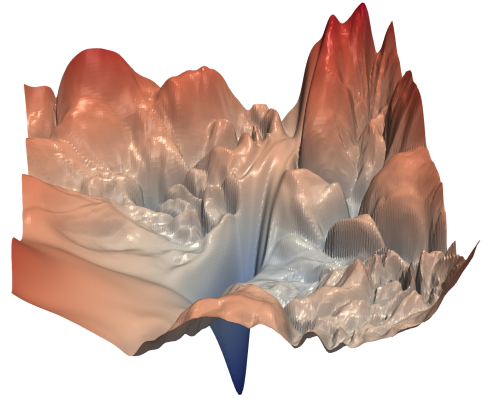
\includegraphics[width=\linewidth]{img/experiments/landscapemultimodal.png}
    \end{minipage}
    \hfill
    \begin{minipage}{0.49\textwidth}
        \centering
        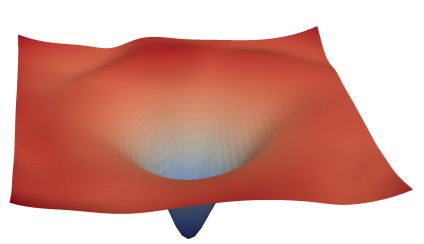
\includegraphics[width=\linewidth]{img/experiments/landscapeunimodal.png}
    \end{minipage}
    \caption[Paisajes de la función de pérdida para distintos modelos sobreparametrizados~\cite{Li2018}.]{Paisajes de la función de pérdida para un modelo sobreparametrizado sin conexiones residuales (izquierda) y con conexiones residuales (derecha)~\cite{Li2018}. A la izquierda, se observa un único mínimo global en un entorno altamente multimodal. A la derecha, se observa un único mínimo global en un entorno unimodal, fruto de las conexiones residuales.}\label{fig:landscapes}
\end{figure} 

A partir de estos resultados, podemos inferir que el algoritmo de optimización, una vez ha alcanzado una solución prácticamente perfecta (es decir, al encontrar un mínimo, potencialmente global, de la función de pérdida), continúa explorando en busca de soluciones aún mejores. Este proceso, debido a la naturaleza del paisaje multimodal en el que opera, provoca que el modelo pueda salir de dicho mínimo, lo que da lugar a los picos observados, para luego converger hacia otro mínimo potencialmente global.\newline

Además, otro hecho relevante es que la magnitud de estos saltos disminuye progresivamente, lo que sugiere que el modelo, al buscar nuevos mínimos globales, tiende a seleccionar un tipo de soluciones frente a otras. Esta respuesta del modelo puede asociarse al hecho de que, entre todas las soluciones posibles, busca aquella que sea más simple, lo cual, como se ha observado en experimentos previos, suele ser una solución que generaliza bien.\newline

La pregunta ahora sería por qué hemos observado estos resultados, cuando no se muestran de manera prominente en la literatura científica. En primer lugar, en los estudios que presentan gráficas de error con el fenómeno del doble descenso, generalmente se utilizan arquitecturas que incluyen conexiones residuales. Este tipo de arquitecturas, según lo demuestran Li et al.~\cite{Li2018}, no presentan paisajes de la función de pérdida multimodales. En cambio, exhiben zonas planas alrededor de los mínimos, impidiendo los saltos bruscos observados en nuestro caso (véase imagen derecha de la Figura~\ref{fig:landscapes}). Así, los mínimos globales se asemejan a los mínimos locales de las zonas infraparametrizadas, lo que impide que el algoritmo de optimización escape de ellos.\newline

Por otra parte, siguiendo los distintos resultados presentados en la Sección~\ref{subsec:model-epoch-wise}, podemos observar que el aumento en el número de parámetros en comparación con el número de ejemplos de entrenamiento, junto con el uso de un conjunto de entrenamiento más difícil (en nuestro caso, conjuntos con imágenes en formato RGB), favorecen la aparición de estas colinas en las gráficas de error.\newline

Finalmente, podemos concluir que, a medida que avanzan las épocas de entrenamiento, estos picos se vuelven cada vez menos notables, posiblemente porque el modelo encuentra cada vez soluciones más simples. Esto podría sugerir que, si se entrenara durante un mayor número de épocas, estos picos podrían llegar a desaparecer por completo.\newline

\endinput
%------------------------------------------------------------------------------------
% FIN DEL APÉNDICE. 
%------------------------------------------------------------------------------------

% !TeX root = ../tfg.tex
% !TeX encoding = utf8

\chapter{Irregularidades en la Dinámica del Error}\label{ap:apendiceD}

En este apéndice analizamos en detalle los saltos bruscos que se producen tanto en el error de entrenamiento como en el de test al aumentar el número de épocas de un determinado modelo, intentando proporcionar una explicación para los mismos.\newline

Nos centramos en la gráfica de la Figura~\ref{fig:model-epoch3CNNCIFAR10}, donde estos picos en el error son más sobresalientes. A partir de esta representación, se analiza el \textit{epoch-wise double descent} en dos modelos que la conforman: uno infraparametrizado, ubicado antes del umbral de interpolación, y otro sobreparametrizado, situado después de dicho umbral.\newline

\begin{figure}[h]
    \centering
    \begin{subfigure}[b]{\textwidth}
        \centering
        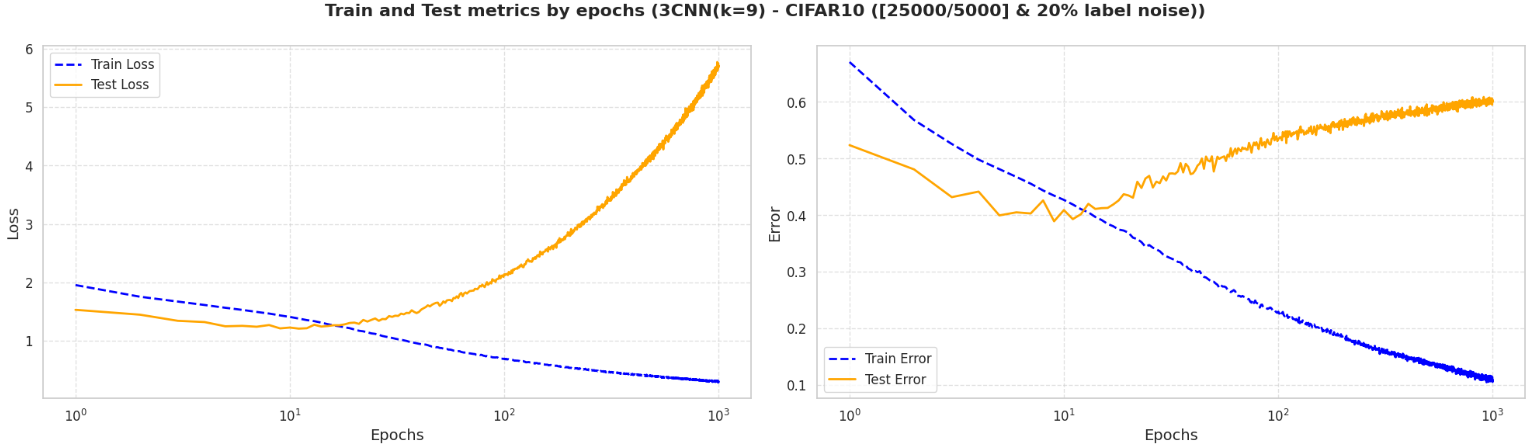
\includegraphics[width=0.9\textwidth]{img/experiments/epoch-wise3CNNunderparameterized.png}
        \caption{A la izquierda, se muestra la pérdida en entrenamiento y test, y a la derecha, el error en entrenamiento y test para un modelo $3$CNN infraparametrizado ($k=9$) sobre el subconjunto CIFAR$10$[$25000/5000$], con $20\%$ de ruido añadido y un \text{batch size} de $128$.}\label{fig:epoch-wise3CNNunderparameterized}
    \end{subfigure}
    
    \vspace{1em} 

    \begin{subfigure}[b]{\textwidth}
        \centering
        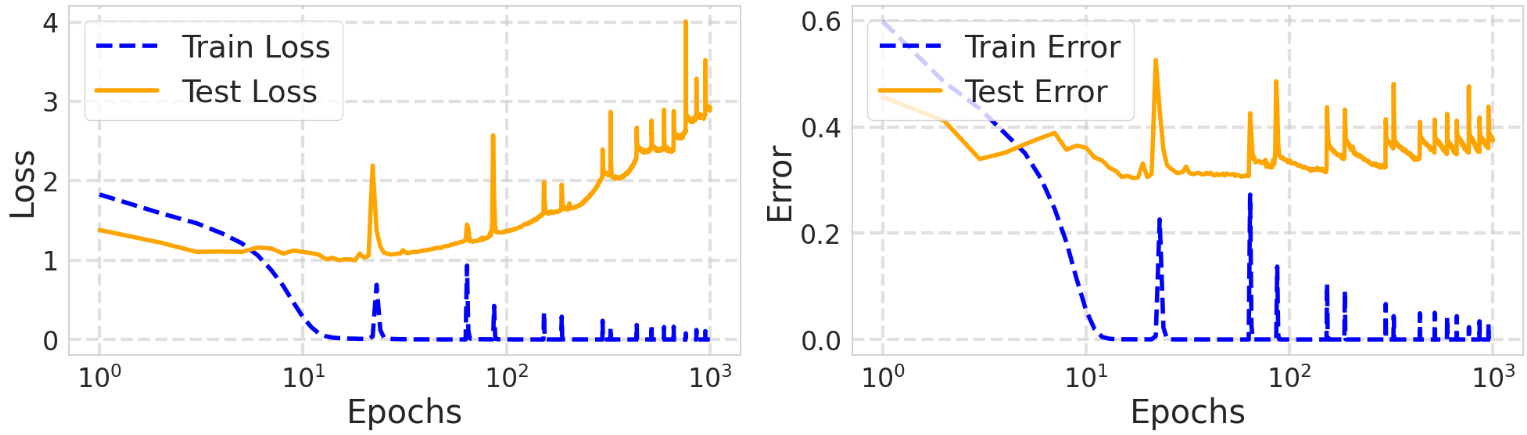
\includegraphics[width=0.9\textwidth]{img/experiments/epoch-wise3CNNoverparameterized.png}
        \caption{A la izquierda, se muestra la pérdida en entrenamiento y test, y a la derecha, el error en entrenamiento y test para un modelo $3$CNN sobreparametrizado ($k=60$) sobre el subconjunto CIFAR$10$[$25000/5000$], con $20\%$ de ruido añadido y un \text{batch size} de $128$. Se aprecian variaciones abruptas tanto en la gráfica de la pérdida como en la del error.}\label{fig:epoch-wise3CNNoverparameterized}
    \end{subfigure}
    
    \caption[Comparativa \textit{epoch-wise double descent} entre un modelo infraparametrizado y uno sobreparametrizado en el que aparecen picos significativos en el error.]{Comparativa \textit{epoch-wise double descent} entre un modelo infraparametrizado, donde no se observa el doble descenso, y un modelo sobreparametrizado, en el que este efecto sí se manifiesta y aparecen picos significativos en el error.}\label{fig:epoch-wise-bruscos1}
\end{figure}

Para intentar dar una explicación coherente a la conducta, ciertamente peculiar, que se observa en estas gráficas, recordemos algunos de los resultados presentados en la Sección~\ref{sec:optimizacion-zona-sobreparametrizada}. En la zona infraparametrizada, sabemos que los mínimos locales suelen estar aislados, lo que provoca que el paisaje de la función de pérdida en sus alrededores sea localmente convexo (véase imagen izquierda de la Figura~\ref{fig:localglobalminima}).\newline

Debido a esto, la inicialización del optimizador juega un papel crucial, ya que determinará hacia qué mínimo local convergerá. En particular, el optimizador tiende a dirigirse hacia el mínimo local más cercano a su punto de inicio. Dado que la región circundante es localmente convexa, el optimizador avanzará progresivamente hacia dicho mínimo sin posibilidad de escapar de él, siempre que la tasa de aprendizaje sea adecuada. Este comportamiento explica por qué, en la zona infraparametrizada, la pérdida en entrenamiento sigue una tendencia descendente y converge de manera estable. Al no haber direcciones de escape significativas, el optimizador se mantiene atrapado en el mínimo local alcanzado, lo que se traduce en una reducción progresiva y sostenida de la pérdida a lo largo del proceso de optimización. Sin embargo, debido a la limitada capacidad del modelo en esta región, el error en el conjunto de test permanece elevado, reflejando una falta de flexibilidad para ajustarse adecuadamente a los datos (véase Figura~\ref{fig:epoch-wise3CNNunderparameterized}).\newline

En cambio, en la zona sobreparametrizada, los mínimos globales no están aislados, sino que en cualquier pequeña vecindad de ellos siempre es posible encontrar otro minimizador global (véase Sección~\ref{sec:optimizacion-zona-sobreparametrizada}). Esto implica que la función de pérdida presenta una alta no convexidad, incluso a nivel local. Como resultado, el paisaje de la función de pérdida en estos modelos es multimodal, como se ilustra en la imagen izquierda de la Figura~\ref{fig:landscapes}. Aunque dicha imagen muestre únicamente un mínimo global en un espacio tridimensional, es importante recordar que existen múltiples de ellos en las dimensiones definidas por el espacio de parámetros. En otras palabras, paisajes similares a este (aunque más complejos debido a su alta dimensionalidad) se replicarían en distintas regiones del espacio de parámetros, dando lugar a un paisaje altamente multimodal con una multitud de mínimos globales.\newline 

\begin{figure}[h!]
    \centering
    \begin{minipage}{0.49\textwidth}
        \centering
        \includegraphics[width=\linewidth]{img/experiments/landscapemultimodal.png}
    \end{minipage}
    \hfill
    \begin{minipage}{0.49\textwidth}
        \centering
        \includegraphics[width=\linewidth]{img/experiments/landscapeunimodal.png}
    \end{minipage}
    \caption[Paisajes de la función de pérdida para distintos modelos sobreparametrizados~\cite{Li2018}.]{Paisajes de la función de pérdida para un modelo sobreparametrizado sin conexiones residuales (izquierda) y con conexiones residuales (derecha)~\cite{Li2018}. A la izquierda, se observa un único mínimo global en un entorno altamente multimodal. A la derecha, se observa un único mínimo global en un entorno unimodal, fruto de las conexiones residuales.}\label{fig:landscapes}
\end{figure} 

A partir de estos resultados, podemos inferir que el algoritmo de optimización, una vez ha alcanzado una solución prácticamente perfecta (es decir, al encontrar un mínimo, potencialmente global, de la función de pérdida), continúa explorando en busca de soluciones aún mejores (en términos de generalización). Este proceso, debido a la naturaleza del paisaje multimodal en el que opera, provoca que el modelo pueda salir de dicho mínimo, lo que da lugar a los picos observados, para luego converger hacia otro mínimo potencialmente global.\newline

Además, otro hecho relevante es que la magnitud de estos saltos disminuye progresivamente, lo que sugiere que el modelo, al buscar nuevos mínimos globales, tiende a seleccionar un tipo de soluciones frente a otras. Esta respuesta del modelo puede asociarse al hecho de que, entre todas las soluciones posibles, busca aquella que sea más simple, lo cual, como se ha observado en experimentos previos, suele ser una solución que generaliza bien.\newline

La pregunta ahora sería por qué hemos observado estos resultados, cuando no se muestran de manera prominente en la literatura científica. En primer lugar, en los estudios que presentan gráficas de error con el fenómeno del doble descenso, generalmente se utilizan arquitecturas que incluyen conexiones residuales. Este tipo de arquitecturas, según lo demuestran Li et al.~\cite{Li2018}, no presentan paisajes de la función de pérdida multimodales. En cambio, exhiben zonas planas alrededor de los mínimos, impidiendo los saltos bruscos observados en nuestro caso (véase imagen derecha de la Figura~\ref{fig:landscapes}). Así, los mínimos globales se asemejan a los mínimos locales de las zonas infraparametrizadas, lo que impide que el algoritmo de optimización escape de ellos.\newline

Por otra parte, siguiendo los distintos resultados presentados en la Sección~\ref{subsec:model-epoch-wise}, podemos observar que el aumento en el número de parámetros en comparación con el número de ejemplos de entrenamiento, junto con el uso de un conjunto de entrenamiento más difícil (en nuestro caso, conjuntos con imágenes en formato RGB), favorecen la aparición de estas colinas en las gráficas de error.\newline

Finalmente, podemos concluir que, a medida que avanzan las épocas de entrenamiento, estos picos se vuelven cada vez menos notables, posiblemente porque el modelo encuentra cada vez soluciones más simples. Esto sugiere que, si se entrenara durante un mayor número de épocas de entrenamiento, estos picos podrían llegar a ser prácticamente imperceptibles o incluso desaparecer por completo.\newline

\endinput
%------------------------------------------------------------------------------------
% FIN DEL APÉNDICE. 
%------------------------------------------------------------------------------------

% Añadir tantos apéndices como sea necesario 

% -------------------------------------------------------------------
% GLOSARIO: Opcional
% -------------------------------------------------------------------

% !TeX root = ../tfg.tex
% !TeX encoding = utf8

\chapter*{Glosario}
\addcontentsline{toc}{chapter}{Glosario} % Añade el glosario a la tabla de contenidos

\begin{description} 
  \item[$\mathbb{R}$] Conjunto de números reales.
  \item[$\mathbb{N}$] Conjunto de números naturales.
  \item[i.d.d.] Independientes e idénticamente distribuidas.
  \item[${\mathbb{E}[X]}$] Esperanza de la variable aleatoria $X$.
  \item[${P[X, Y]}$] Probabilidad conjunta de las variables aleatorias $X$ e $Y$.
  \item[SVD] Descomposición en valores singulares.
  \item[$X^{\dagger}$] Pseudoinversa de la matriz $X$.
  \item[Descenso de gradiente] Método de optimización utilizado para minimizar una función de pérdida.
  \item[$\mathcal{H}$] Conjunto de hipótesis de un modelo formado por las hipótesis candidatas y la función objetivo.
  \item[$\mathcal{D}$] Conjunto de datos de entrenamiento.
  \item[$E_{out}$] Error fuera de la muestra o error de generalización. 
  \item[$E_{in}$] Error dentro de la muestra o error de entrenamiento.
  \item[Complejidad efectiva del modelo] Máximo número de ejemplos de entrenamiento en el que el modelo obtiene un $E_{in}$ próximo a cero.
\end{description}
\endinput
 

% -------------------------------------------------------------------
% BACKMATTER
% -------------------------------------------------------------------

\backmatter % Desactiva la numeración de los capítulos
\pdfbookmark[-1]{Referencias}{BM-Referencias}

% BIBLIOGRAFÍA
%-------------------------------------------------------------------

\bibliographystyle{alpha-es} 
\begin{small} 
  \bibliography{library.bib}
\end{small}


\end{document}
